% WACV 2024 Paper Template
% based on the CVPR 2023 template (https://media.icml.cc/Conferences/CVPR2023/cvpr2023-author_kit-v1_1-1.zip) with 2-track changes from the WACV 2023 template (https://github.com/wacv-pcs/WACV-2023-Author-Kit)
% based on the CVPR template provided by Ming-Ming Cheng (https://github.com/MCG-NKU/CVPR_Template)
% modified and extended by Stefan Roth (stefan.roth@NOSPAMtu-darmstadt.de)

\documentclass[10pt,twocolumn,letterpaper]{article}

%%%%%%%%% PAPER TYPE  - PLEASE UPDATE FOR FINAL VERSION
%\usepackage[review,algorithms]{wacv}      % To produce the REVIEW version for the algorithms track
%\usepackage[review,applications]{wacv}      % To produce the REVIEW version for the applications track
\usepackage{wacv}              % To produce the CAMERA-READY version
%\usepackage[pagenumbers]{wacv} % To force page numbers, e.g. for an arXiv version

% Include other packages here, before hyperref.
\usepackage{graphicx}
\usepackage{amsmath}
\usepackage{amssymb}
\usepackage{booktabs}

\usepackage{caption}
\usepackage{subcaption}
\usepackage{tikz}
\usepackage{multicol}

% It is strongly recommended to use hyperref, especially for the review version.
% hyperref with option pagebackref eases the reviewers' job.
% Please disable hyperref *only* if you encounter grave issues, e.g. with the
% file validation for the camera-ready version.
%
% If you comment hyperref and then uncomment it, you should delete
% ReviewTempalte.aux before re-running LaTeX.
% (Or just hit 'q' on the first LaTeX run, let it finish, and you
%  should be clear).
\usepackage[pagebackref,breaklinks,colorlinks]{hyperref}


% Support for easy cross-referencing
\usepackage[capitalize]{cleveref}
\crefname{section}{Sec.}{Secs.}
\Crefname{section}{Section}{Sections}
\Crefname{table}{Table}{Tables}
\crefname{table}{Tab.}{Tabs.}


%%%%%%%%% PAPER ID  - PLEASE UPDATE
\def\wacvPaperID{1589} % *** Enter the WACV Paper ID here
\def\confName{WACV}
\def\confYear{2024}


\newcommand*{\affaddr}[1]{#1} % No op here. Customize it for different styles.
\newcommand*{\affmark}[1][*]{\textsuperscript{#1}}
\newcommand*{\email}[1]{\texttt{#1}}

\begin{document}

%%%%%%%%% TITLE - PLEASE UPDATE
\title{Self-Supervised Video Transformers for Isolated Sign Language Recognition}

\author{%
Marcelo Sandoval-Casta\~neda\affmark[1]\affmark[*], Yanhong Li\affmark[2], Diane Brentari\affmark[2], Karen Livescu\affmark[1], and Gregory Shakhnarovich\affmark[1]\\
\affaddr{\affmark[1]Toyota Technological Institute at Chicago, IL, USA}\\
\affaddr{\affmark[2]University of Chicago, IL, USA}\\
\email{\affmark[*]marcelo@ttic.edu}\\
}



\maketitle

%%%%%%%%% ABSTRACT
\begin{abstract}
   This paper presents an in-depth analysis of various self-supervision methods for isolated sign language recognition (ISLR). We consider four recently introduced transformer-based approaches to self-supervised learning from videos, and four pre-training data regimes, and study all the combinations on the WLASL2000 dataset.
   %We scrutinize four different self-supervised transformer models: VideoMAE, SVT, BEVT, and MaskFeat, each pre-trained under four distinct settings: Kinetics400 pre-training, OpenASL pre-training, two-stage pre-training (first on Kinetics400, then extended with OpenASL), and mixed pre-training (Kinetics400 and OpenASL at the same time). We evaluate the performance of these models on WLASL2000 after fine-tuning.
   Our findings reveal that MaskFeat achieves performance superior to pose-based and supervised video models, with a top-1 accuracy of 79.02\% on gloss-based WLASL2000. Furthermore, we analyze these models' ability to produce representations of ASL signs using linear probing on diverse phonological features. This study underscores the value of architecture and pre-training task choices in ISLR. Specifically, our results on WLASL2000 highlight the power of masked reconstruction pre-training, and our linear probing results demonstrate the importance of hierarchical vision transformers for sign language representation.
\end{abstract}


%%%%%%%%% BODY TEXT
\section{Introduction}
\label{sec:intro}

American Sign Language (ASL) is the predominant language of Deaf communities in the United States, with an estimated 500,000 native users~\cite{ethnologue}. However, natural language processing has largely focused on spoken and written language only~\cite{yin2021including}. Recently, there is an increasing body of work in NLP tasks related to sign language, with particular focus on isolated sign language recognition (ISLR) and sign language translation (SLT).

In ISLR, the input consists of dictionary-style videos which have only one signer articulating one individual sign, and the task is to classify this video according to the sign label. Figure~\ref{fig:wlasl-samples} shows frames extracted from such videos, which are typically two or three seconds long, have a solid color background, and show people signing while standing facing the camera. ISLR labels are usually words in English or sign language glosses, which are typically a combination of morpheme translations into English along with differentiating phonological features like handshape and location.

\begin{figure}
    \centering
    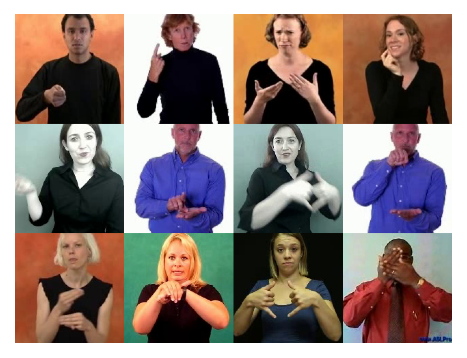
\includegraphics[width=\linewidth]{figures/wlasl-samples.pdf}
    \caption{Sample frames from isolated sign language video extracted from the WLASL2000 dataset~\cite{Li2020WLASL}.}
    \label{fig:wlasl-samples}
\end{figure}

On the other hand, in SLT the input consists of videos that contain continuous signing, and the task is to produce (usually text) translations in a given target language, typically the lingua franca of the region where the source sign language is predominant or English. The sources of these videos are highly variable, ranging from news sources to personal video blogs. Figure~\ref{fig:oasl-samples} shows example frames from sign language translation videos. Unlike ISLR, these videos are significantly longer, and can include all sorts of backgrounds, positions, and number of people, depending on the source it was extracted from.

\begin{figure}
    \centering
    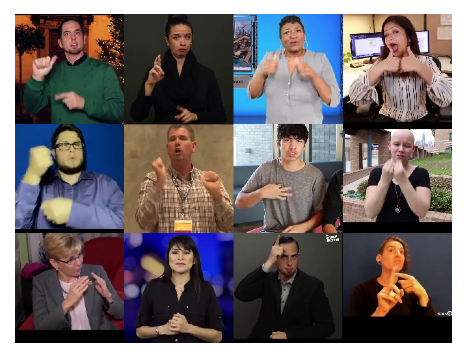
\includegraphics[width=\linewidth]{figures/oasl-samples.pdf}
    \caption{Sample frames extracted from ASL to English translation dataset OpenASL~\cite{Shi2022OpenASL}.}
    \label{fig:oasl-samples}
\end{figure}

In this paper, we focus on ISLR as a task to evaluate our models, as translation remains extremely difficult, with very poor state-of-the-art performance. Moreover, SLT models often rely on ISLR models as feature extractors~\cite{chen2022simple,muller2022findings,shi2022ttic}. Despite their usage in a language task, these models have not yet been evaluated in their ability to encode linguistically relevant features. In the case of sign languages, Brentari's prosodic model of sign language phonology~\cite{brentari1998prosodic} provides a set of phonological features that can uniquely characterize up to 70\% of signs in ASL~\cite{sehyr2021asllex}. These encode multiple characteristics of all signs, such as handshapes, movement, and symmetry.

Naturally, the most common modality of sign language data is video. Current state-of-the-art video classification tasks are dominated by vision transformers. Recent advances in this area have come from various self-supervised pre-training tasks, especially when dealing with smaller classification datasets. These are either based on some form of contrastive pre-training~\cite{pan2021videomoco,Kuang_2021_ICCV,Ranasinghe2021SVT} or masked reconstruction~\cite{Tong2022VideoMAE,Wang2021BEVT,Wei2022MaskFeat}, following the nature of advances in other fields like text, single images, and speech. These self-supervision methods have not yet been explored for sign language tasks. Self-supervision requires large datasets to function effectively, and large sign language datasets did not exist until very recently. In this paper, we study multiple video transformers and self-supervision settings to understand the effect of self-supervision for sign language processing tasks.

The contributions of this paper are the following:
\begin{itemize}
    \item \textbf{Establish a new state of the art on gloss-based WLASL2000.} MViTv2 with MaskFeat pre-training achieves 79.02\% accuracy, surpassing pose-based state of the art by 1.59\%.
    \item \textbf{Evaluate the effect of multiple self-supervision tasks on ISLR performance.} We compare pixel reconstruction (VideoMAE~\cite{Tong2022VideoMAE}), feature reconstruction (MaskFeat~\cite{Wei2022MaskFeat}), BERT pre-training for videos (BEVT~\cite{Wang2021BEVT}), and DINO pre-training for videos (SVT~\cite{Ranasinghe2021SVT}).
    \item \textbf{Introduce phonological features as a tool to analyze sign language representations produced by self-supervised models.} We use this to better characterize the strengths and limitations of architectures and pre-training tasks.
\end{itemize}


\section{Related Work}
\label{sec:related-work}

\subsection{Isolated Sign Language Recognition}
\label{sec:related-work-islr}

The most common approach to ISLR is based on convolutional neural networks (CNNs), such as I3D~\cite{carreira2017quo}, R3D~\cite{hara2017learning}, and S3D~\cite{xie2018rethinking}. These models receive RGB videos as input, extract features from them, and use these features to assign a label for the corresponding sign~\cite{Albanie2020BSL1K, Varol2021BSL1KImp, zuo2023natural}. Other approaches employ pose-based models to mitigate variations naturally present in video that are not related to the task of identifying signs~\cite{jiang2021skeleton, jiang2021sign, Dafnis2022Bidirectional}.

Choosing the right pre-training tasks and set-ups has largely been the determining factor in ISLR performance, all of which involve supervision on other datasets. The most common pre-training datasets include Kinetics400~\cite{carreira2017quo} and larger isolated sign language datasets in a language different from the target~\cite{Albanie2020BSL1K, Varol2021BSL1KImp, Novopoltsev2023Finetuning}. Recent approaches also include auxiliary tasks during ISLR training. These include weakly-supervised phonological features~\cite{kezar2023improving} and word embeddings from written language models~\cite{zuo2023natural}.

Our approach is most similar to~\cite{Novopoltsev2023Finetuning}, which uses a VideoSwin transformer with supervised pre-training on human action recognition with Kinetics400, then Russian Sign Language ISLR with a proprietary dataset, and finally fine-tuning on WLASL2000. In contrast, we pre-train on either human action videos or exclusively on ASL videos (or a combination of both) in a self-supervised manner, and then fine-tune for ISLR on WLASL2000.

\subsection{Self-Supervised Video Transformers}
\label{sec:related-work:-self-supervised-video-transformers}

In video self-supervision with transformers, there are four dominant approaches that can be broadly summarized by their choice of objective during pre-training:
masked reconstruction of pixels~\cite{Tong2022VideoMAE, feichtenhofer2022maest, Wang2023VideoMAE2}, DINO-based~\cite{caron2021emerging} representation learning using a teacher-student setup~\cite{Ranasinghe2021SVT, wang2022mvd}, masked reconstruction of hand-crafted features, most often HOG,~\cite{Wei2022MaskFeat, sun2023mme}, and BERT-like~\cite{devlin2018bert} masked token prediction using codewords generated by a discrete VAE~\cite{Wang2021BEVT, tan2021VIMPAC}. We choose one model from each category, specifically VideoMAE~\cite{Tong2022VideoMAE} for masked reconstruction over pixels, SVT~\cite{Ranasinghe2021SVT} for DINO-like representation learning, MaskFeat~\cite{Wei2022MaskFeat} for masked reconstruction over HOG, and BEVT~\cite{Wang2021BEVT} for BERT-like masked token prediction.

Additionally, there has also been a significant amount of work on custom architectures for vision transformers. ViT~\cite{dosovitskiy2020image} remains the most common architecture, which uses standard multi-head attention~\cite{vaswani2017attention}, with a fixed patch size of $16 \times 16$ pixels. Other custom architectures for vision have been proposed recently, most importantly VideoSwin~\cite{liu2022video} and MViT~\cite{fan2021multiscale, li2022mvitv2}. These use modified multi-head attention modules: window-based attention for VideoSwin and pooling attention for MViT, with much smaller input patches of $4 \times 4$ pixels. Our model choices also reflect this landscape, since VideoMAE and SVT are based on ViT, BEVT is based on VideoSwin, and MaskFeat is based on MViTv2.


\section{Method}
\label{sec:method}

For our experiments, we select one model from each method identified in Section~\ref{sec:related-work:-self-supervised-video-transformers}. We take the best performing architecture and set-up described in their respective papers.

{\bf VideoMAE~\cite{Tong2022VideoMAE}.} We pre-train a standard ViT with masked reconstruction over pixels, where the masked regions are tubes across time (i.e. the same 2D mask is applied to every frame), and with an extremely high masking ratio of 90\%. As a standard ViT, this model divides frames into patches of $16 \times 16$ pixels.

{\bf SVT~\cite{Ranasinghe2021SVT}.} We extend a standard ViT previously DINO pre-trained on ImageNet with further DINO pre-training on video. That is, we take a mean teacher~\cite{tarvainen2017mean} with a global view of the data and a student with narrower spatio-temporal slices, and the objective of the student is to produce representations from these narrower views that are as close as possible to the mean teacher. As a standard ViT, its patch size is $16 \times 16$ pixels.

{\bf MaskFeat~\cite{Wei2022MaskFeat}.} We pre-train a MViTv2 model for masked reconstruction over HOG, where the masked regions are segments over time of up to half the video length, composed of multiple adjacent patches, and with a much lower masking ratio compared to VideoMAE, 40\%. As a MViT-based model, the patch size is $4 \times 4$ pixels.

{\bf BEVT~\cite{Wang2021BEVT}.} We train a VideoSwin to predict labels or ``words'' for masked regions in a video. These labels are generated by the codebook of an external discrete VAE (dVAE), separately trained on Conceptual Captions~\cite{sharma2018conceptual} as part of DALL-E~\cite{ramesh2021zero}. The masking strategy is the same as in MaskFeat, but with a slightly higher masking ratio of 50\%. VideoSwin also takes as input patches of $4 \times 4$ pixels.

\section{Experimental Setup}
\label{sec:experimental-setup}

\subsection{Datasets}
\label{sec:experimental-setup-datasets}

We rely on four different datasets, two for pre-training, one for fine-tuning, and one for linear probing of phonological features.

The first of these is Kinetics400~\cite{carreira2017quo}, the de facto standard dataset of human action videos. It contains 400 categories of human actions, with around 600 hours of video in total. We use it exclusively for self-supervised pre-training, ignoring the labels of the videos.

Additionally, we use OpenASL~\cite{Shi2022OpenASL}, one of the largest and most diverse ASL translation datasets, with 288 hours of ASL videos paired with English text translation and more than 200 signers. Since we only use it for self-supervised pre-training, we use OpenASL videos without their subtitle counterparts.

We fine-tune all of our models using WLASL2000~\cite{Li2020WLASL}. The original version of this dataset consisted of 14 hours of isolated sign language videos in ASL, with 2000 labels in total. However, recent analysis of this dataset~\cite{Dafnis2022Bidirectional} revealed major weaknesses and inconsistencies that are a product of relying on English translations as sign names. For this reason, we use the manually-corrected version of WLASL2000~\cite{neidle2022alternative}, with only 1535 labels based on ASL glosses instead of English translations and 12 hours of video.

For our linear probing experiments, we draw from sign language phonology, that is, the study of abstract grammatical components that are combined into meaningful utterances~\cite{brentari2019sign}. We extend the gloss-based WLASL2000 labels with phonological features extracted from ASL-LEX 2.0~\cite{sehyr2021asllex}. Due to inconsistent labeling across datasets and dialect variations, we only map a subset of 916 WLASL labels with their corresponding features where an unambiguous correspondence can be found. That is, we strip the morpheme translation part of each gloss label from both WLASL2000 and ASL-LEX 2.0, and only map one to another when there is a unique exact match. This is partially inspired by previous work~\cite{tavella2022wlasl,kezar2023improving}, with two key differences. First, we rely on manually labeled glosses instead of treating the original WLASL2000 labels as gloss approximations, and second, we do not use these additional features as a weak supervision signal, but as a tool help us characterize our self-supervised models.

For a detailed description of each phonological feature used in this study, see Table~\ref{tab:phono-features-description}. Note that the number of classes in Table~\ref{tab:phono-features-description} might be smaller than the original ASL-LEX 2.0 labels, as a product of unambiguous data available in WLASL2000. Additionally, Table~\ref{tab:phono-categorization} groups the phonological features we extract from ASL-LEX 2.0 into broad categories according to the aspect they describe.

\begin{table*}[]
\centering
\begin{tabular}{llc}
\hline
\textbf{Feature} & \textbf{Description} & \textbf{Classes} \\
\hline
Sign Type & Describes whether a sign is one-handed or two-handed and its symmetry properties. & 6 \\
Major Location & General location of the dominant hand in relation to the body. & 5 \\
First Minor Location & Subdivisions within each minor location except ``neutral'' location. & 35 \\
Second Minor Location & Used when the dominant hand moves while signing. & 30 \\
Contact & Describes whether the dominant hand touches the major location during signing. & 2 \\
Handshape & Shape of the dominant signing hand. & 49 \\
Non-Dom. Handshape & Shape of the non-dominant hand. & 45 \\
Selected Fingers & Describes combinations of finger movement and position in the dominant hand. & 10 \\
Flexion & Describes selected finger positions at morpheme onset. & 8 \\
Thumb Position & Describes whether the thumb is in contact with other fingers in the dominant hand. & 2 \\
Path Movement & Path followed by the dominant hand. & 8 \\
Wrist Twist & Describes whether ulnar rotation is present in a sign's movement. & 2 \\
Repeated Movement & Describes whether a sign involves movement repetition of any kind. & 2 \\
\hline
\end{tabular}
\caption{Description of all phonological features used in this study.}
\label{tab:phono-features-description}
\end{table*}

\begin{table}[]
\centering
\begin{tabular}{ll}
\hline
\textbf{Main Category} & \textbf{Features} \\
\hline
Sign Type & Sign Type \\
\hline
Location & Major Location, Minor Location, \\
  &Second Minor Location, Contact \\
\hline
Hand Configuration & Thumb Position, Flexion, \\
  &Handshape, Selected Fingers, \\
    & Non-dominant Handshape \\
\hline
Movement & Path Movement, Wrist Twist, \\
  & Repeated Movement \\
\hline
\end{tabular}
\caption{Broad cateogrization of phonological features included in this study.}
\label{tab:phono-categorization}
\end{table}

\subsection{Pre-Training}
\label{sec:experimental-setup-pretraining}

For each of our four models, we explore four pre-training configurations. The first is to pre-train each model in Kinetics400 using the pre-training setup and hyperparameters from the model's original paper. The second is to keep the setup and hyperparameters, but replace Kinetics400 with OpenASL. Our third configuration is to first pre-train the model on Kinetics400 as in the corresponding paper, and add a second pre-training stage on OpenASL, with all the hyperparameters staying the same except learning rate, which we instead reduce to a tenth of the original. Last, our fourth configuration is to pre-train a model on the union of Kinetics400 and OpenASL, keeping each model's original pre-training setup and hyperparameters.


\subsection{Evaluation}
\label{sec:experimental-setup-evaluation}

To evaluate our models, we conduct fine-tuning and layer-wise linear probing. We fine-tune on the gloss-based version of WLASL2000, and compare models by top-1 accuracy. For linear probing, we freeze the model and train softmax classifiers with the output of each layer as input, as an attempt to measure whether phonological features are encoded well in our trained models. We do so before and after fine-tuning on WLASL2000. This is inspired by previous work that analyzes linguistic properties of speech models~\cite{pasad2021layer,ji2022predicting,pasad2023comparative}. We select the models to analyze based on ISLR fine-tuning performance.


\section{Experimental Results}
\label{sec:experimental-results}

\subsection{Fine-Tuning}
\label{sec:experimental-results-fine-tuning}

Our fine-tuning results can be found in Table~\ref{tab:wlasl-performance}. We include the results of pose-based Bi-GCN on gloss-based WLASL2000, as reported in~\cite{Dafnis2022Bidirectional}, which is state of the art in the gloss-based setup. Additionally, we report results from video-based I3D models with supervised pre-training~\cite{Albanie2020BSL1K, Varol2021BSL1KImp}, which is state of the art on the original WLASL2000 with publicly available datasets and without additional signals, and that we train on gloss-based WLASL2000 for this paper.

We can see in Table~\ref{tab:wlasl-performance} that there is no clear superior pre-training dataset combination across all models and pre-training tasks. Both models that deal with reconstruction over masked regions, VideoMAE and MaskFeat, benefit from the combination of Kinetics and OpenASL. However, they favour different datasets in our single-dataset setting, albeit with similar behaviour for their respective performances. In the case of VideoMAE, OpenASL pre-training achieves much lower accuracy than that of Kinetics400 pre-training (16.19 vs. 67.25), and the benefit of our two-stage pretraining results in an increase of 2.07 after pre-training on both Kinetics400 and OpenASL. For MaskFeat, this is inverted: Kinetics400-only pre-training yields an accuracy of 12.50, much lower than OpenASL-only at 74.68. Two-stage pre-training pushes this number further, up to 79.02, 4.34 points above the best single-dataset MaskFeat. We hypothesize that these differences can be at least partially attributable to the pre-training objective. HOG may allow the model to mitigate the less-relevant variation over pixels, while focusing on aspects that are more important to sign language and are captured by HOG, especially shapes.

\begin{table}[]
\centering
\begin{tabular}{lcc}
\hline
\textbf{Model} & \textbf{Pre-Training} & \textbf{Top 1 Acc.} \\
\hline
\textit{Bi-GCN} & \textit{Pose} & \textit{77.43} \\
\textit{I3D} & \textit{K400 (Sup.)} & \textit{55.02} \\
\textit{I3D} & \textit{BSL-1K (Sup.)} & \textit{67.60} \\
\hline
VideoMAE & No Pre-Training & 0.47 \\
VideoMAE & K400 & 67.25 \\
VideoMAE & OpenASL & 16.19 \\
VideoMAE & Two-Stage & 69.32 \\
VideoMAE & Mixed & 59.28 \\
\hline
SVT & No Pre-Training & 8.52 \\
SVT & K400 & 19.34 \\
SVT & OpenASL & 13.36 \\
SVT & Two-Stage & 16.06 \\
SVT & Mixed & 11.22 \\
\hline
MaskFeat & No Pre-Training & 1.17 \\
MaskFeat & K400 & 12.50 \\
MaskFeat & OpenASL & 74.68 \\
\textbf{MaskFeat} & \textbf{Two-Stage} & \textbf{79.02} \\
MaskFeat & Mixed & 75.74 \\
\hline
BEVT & No Pre-Training & 0.47 \\
BEVT & K400 & 53.07 \\
BEVT & OpenASL & 60.73 \\
BEVT & Two-Stage & 58.69 \\
BEVT & Mixed & 59.63 \\
\hline
\end{tabular}
\caption{Top 1 accuracy on gloss-based WLASL2000 after fine-tuning for various models and pre-training datasets. Bi-GCN and I3D in \textit{italics} are supervised classification pre-training and pose-based baselines for reference. We take the best-performing word-based WLASL I3D setups and train them for gloss-based WLASL instead. Best performing model in \textbf{bold}. Two-Stage refers to our configuration where a model is first pre-trained with Kinetics400 and then pre-trained with OpenASL, and Mixed refers to our configuration where a model is trained on both Kinetics400 and OpenASL at the same time.}
\label{tab:wlasl-performance}
\end{table}

On the other hand, BEVT performs worse when combining both Kinetics400 and OpenASL, and the best performance is obtained through OpenASL pre-training only. Since the dVAE used in BEVT is frozen and obtained from training over a more diverse set of images, the addition of Kinetics400 leads to optimizing over code word labels that are entirely irrelevant to the task of ISLR, especially since Kinetics400 is larger than OpenASL. This, in turn, diminishes the final accuracy of BEVT, though not by much (60.73 for OpenASL only, and 58.69 for two-stage pre-training or 59.63 for mixed pre-training).

Lastly, SVT does not achieve comparable performance to our baselines under any setting. This is likely a product of its pre-training procedure: it is not necessarily meaningful to map a global view of a sentence in ASL to a smaller slice, especially across time, of the same sentence (which could be a single sign, or a few sign within the sentence). Therefore, it only manages to reach 19.34 accuracy with Kinetics400, with any OpenASL deteriorating its performance further.

We also find that no model benefits from mixed pre-training from scratch. The reason is model-dependent, but we see this happen across the board. For VideoMAE, we find that mixed pre-training performs significantly worse than both Kinetics400-only and two-stage pre-training. This suggests that VideoMAE benefits from first having a diverse enough set of videos and then narrowing down the domain to sign language in the second stage, as opposed to having a single dataset where sign language is highly represented. For SVT, any inclusion of sign language data deteriorates performance significantly. The case of MaskFeat is similar to the case of VideoMAE, but the improvement found from including Kinetics400 is not as significant as in VideoMAE. For BEVT, mixed pre-training deteriorates performance in comparison to OpenASL as a product of adding unrelated data to the training process, which is also found in the deterioration found in two-stage pre-training.

Some of our models surpass current state-of-the-art I3Ds in ISLR, in particular VideoMAE, pre-trained on Kinetics400 and OpenASL, and MaskFeat, pre-trained on both OpenASL alone and on Kinetics400 and OpenASL, using only a quarter of the frames used in I3D and without requiring additional supervision. Even more so, MaskFeat, on Kinetics400 and OpenASL, manages to perform better than Bi-GCN, which not only relies on external pose estimation, but also uses 150 timesteps for classification.

\subsection{Linear Probing}
\label{sec:experimental-results-linear-probing}

\begin{figure}
    \begin{subfigure}[b]{\linewidth}
        \centering
        \renewcommand\sffamily{}
        %% Creator: Matplotlib, PGF backend
%%
%% To include the figure in your LaTeX document, write
%%   \input{<filename>.pgf}
%%
%% Make sure the required packages are loaded in your preamble
%%   \usepackage{pgf}
%%
%% Also ensure that all the required font packages are loaded; for instance,
%% the lmodern package is sometimes necessary when using math font.
%%   \usepackage{lmodern}
%%
%% Figures using additional raster images can only be included by \input if
%% they are in the same directory as the main LaTeX file. For loading figures
%% from other directories you can use the `import` package
%%   \usepackage{import}
%%
%% and then include the figures with
%%   \import{<path to file>}{<filename>.pgf}
%%
%% Matplotlib used the following preamble
%%   \usepackage{fontspec}
%%   \setmainfont{DejaVuSerif.ttf}[Path=\detokenize{/opt/homebrew/Caskroom/miniforge/base/lib/python3.9/site-packages/matplotlib/mpl-data/fonts/ttf/}]
%%   \setsansfont{DejaVuSans.ttf}[Path=\detokenize{/opt/homebrew/Caskroom/miniforge/base/lib/python3.9/site-packages/matplotlib/mpl-data/fonts/ttf/}]
%%   \setmonofont{DejaVuSansMono.ttf}[Path=\detokenize{/opt/homebrew/Caskroom/miniforge/base/lib/python3.9/site-packages/matplotlib/mpl-data/fonts/ttf/}]
%%
\begingroup%
\makeatletter%
\begin{pgfpicture}%
\pgfpathrectangle{\pgfpointorigin}{\pgfqpoint{3.250000in}{1.250000in}}%
\pgfusepath{use as bounding box, clip}%
\begin{pgfscope}%
\pgfsetbuttcap%
\pgfsetmiterjoin%
\definecolor{currentfill}{rgb}{1.000000,1.000000,1.000000}%
\pgfsetfillcolor{currentfill}%
\pgfsetlinewidth{0.000000pt}%
\definecolor{currentstroke}{rgb}{0.500000,0.500000,0.500000}%
\pgfsetstrokecolor{currentstroke}%
\pgfsetdash{}{0pt}%
\pgfpathmoveto{\pgfqpoint{0.000000in}{0.000000in}}%
\pgfpathlineto{\pgfqpoint{3.250000in}{0.000000in}}%
\pgfpathlineto{\pgfqpoint{3.250000in}{1.250000in}}%
\pgfpathlineto{\pgfqpoint{0.000000in}{1.250000in}}%
\pgfpathlineto{\pgfqpoint{0.000000in}{0.000000in}}%
\pgfpathclose%
\pgfusepath{fill}%
\end{pgfscope}%
\begin{pgfscope}%
\pgfsetbuttcap%
\pgfsetmiterjoin%
\definecolor{currentfill}{rgb}{0.898039,0.898039,0.898039}%
\pgfsetfillcolor{currentfill}%
\pgfsetlinewidth{0.000000pt}%
\definecolor{currentstroke}{rgb}{0.000000,0.000000,0.000000}%
\pgfsetstrokecolor{currentstroke}%
\pgfsetstrokeopacity{0.000000}%
\pgfsetdash{}{0pt}%
\pgfpathmoveto{\pgfqpoint{0.536502in}{0.041670in}}%
\pgfpathlineto{\pgfqpoint{3.208330in}{0.041670in}}%
\pgfpathlineto{\pgfqpoint{3.208330in}{1.208330in}}%
\pgfpathlineto{\pgfqpoint{0.536502in}{1.208330in}}%
\pgfpathlineto{\pgfqpoint{0.536502in}{0.041670in}}%
\pgfpathclose%
\pgfusepath{fill}%
\end{pgfscope}%
\begin{pgfscope}%
\pgfpathrectangle{\pgfqpoint{0.536502in}{0.041670in}}{\pgfqpoint{2.671828in}{1.166660in}}%
\pgfusepath{clip}%
\pgfsetrectcap%
\pgfsetroundjoin%
\pgfsetlinewidth{0.803000pt}%
\definecolor{currentstroke}{rgb}{1.000000,1.000000,1.000000}%
\pgfsetstrokecolor{currentstroke}%
\pgfsetdash{}{0pt}%
\pgfpathmoveto{\pgfqpoint{0.643375in}{0.041670in}}%
\pgfpathlineto{\pgfqpoint{0.643375in}{1.208330in}}%
\pgfusepath{stroke}%
\end{pgfscope}%
\begin{pgfscope}%
\pgfpathrectangle{\pgfqpoint{0.536502in}{0.041670in}}{\pgfqpoint{2.671828in}{1.166660in}}%
\pgfusepath{clip}%
\pgfsetrectcap%
\pgfsetroundjoin%
\pgfsetlinewidth{0.803000pt}%
\definecolor{currentstroke}{rgb}{1.000000,1.000000,1.000000}%
\pgfsetstrokecolor{currentstroke}%
\pgfsetdash{}{0pt}%
\pgfpathmoveto{\pgfqpoint{3.101457in}{0.041670in}}%
\pgfpathlineto{\pgfqpoint{3.101457in}{1.208330in}}%
\pgfusepath{stroke}%
\end{pgfscope}%
\begin{pgfscope}%
\pgfpathrectangle{\pgfqpoint{0.536502in}{0.041670in}}{\pgfqpoint{2.671828in}{1.166660in}}%
\pgfusepath{clip}%
\pgfsetrectcap%
\pgfsetroundjoin%
\pgfsetlinewidth{0.803000pt}%
\definecolor{currentstroke}{rgb}{1.000000,1.000000,1.000000}%
\pgfsetstrokecolor{currentstroke}%
\pgfsetdash{}{0pt}%
\pgfpathmoveto{\pgfqpoint{0.536502in}{0.264826in}}%
\pgfpathlineto{\pgfqpoint{3.208330in}{0.264826in}}%
\pgfusepath{stroke}%
\end{pgfscope}%
\begin{pgfscope}%
\definecolor{textcolor}{rgb}{0.333333,0.333333,0.333333}%
\pgfsetstrokecolor{textcolor}%
\pgfsetfillcolor{textcolor}%
\pgftext[x=0.041670in, y=0.212065in, left, base]{\color{textcolor}\sffamily\fontsize{10.000000}{12.000000}\selectfont 0.400}%
\end{pgfscope}%
\begin{pgfscope}%
\pgfpathrectangle{\pgfqpoint{0.536502in}{0.041670in}}{\pgfqpoint{2.671828in}{1.166660in}}%
\pgfusepath{clip}%
\pgfsetrectcap%
\pgfsetroundjoin%
\pgfsetlinewidth{0.803000pt}%
\definecolor{currentstroke}{rgb}{1.000000,1.000000,1.000000}%
\pgfsetstrokecolor{currentstroke}%
\pgfsetdash{}{0pt}%
\pgfpathmoveto{\pgfqpoint{0.536502in}{0.833811in}}%
\pgfpathlineto{\pgfqpoint{3.208330in}{0.833811in}}%
\pgfusepath{stroke}%
\end{pgfscope}%
\begin{pgfscope}%
\definecolor{textcolor}{rgb}{0.333333,0.333333,0.333333}%
\pgfsetstrokecolor{textcolor}%
\pgfsetfillcolor{textcolor}%
\pgftext[x=0.041670in, y=0.781049in, left, base]{\color{textcolor}\sffamily\fontsize{10.000000}{12.000000}\selectfont 0.600}%
\end{pgfscope}%
\begin{pgfscope}%
\pgfpathrectangle{\pgfqpoint{0.536502in}{0.041670in}}{\pgfqpoint{2.671828in}{1.166660in}}%
\pgfusepath{clip}%
\pgfsetrectcap%
\pgfsetroundjoin%
\pgfsetlinewidth{1.003750pt}%
\definecolor{currentstroke}{rgb}{0.886275,0.290196,0.200000}%
\pgfsetstrokecolor{currentstroke}%
\pgfsetdash{}{0pt}%
\pgfpathmoveto{\pgfqpoint{0.643375in}{0.174795in}}%
\pgfpathlineto{\pgfqpoint{0.750249in}{0.238582in}}%
\pgfpathlineto{\pgfqpoint{0.857122in}{0.306015in}}%
\pgfpathlineto{\pgfqpoint{0.963995in}{0.284145in}}%
\pgfpathlineto{\pgfqpoint{1.070868in}{0.254985in}}%
\pgfpathlineto{\pgfqpoint{1.177741in}{0.411720in}}%
\pgfpathlineto{\pgfqpoint{1.284614in}{0.521070in}}%
\pgfpathlineto{\pgfqpoint{1.391487in}{0.555697in}}%
\pgfpathlineto{\pgfqpoint{1.498360in}{0.754350in}}%
\pgfpathlineto{\pgfqpoint{1.605233in}{0.757995in}}%
\pgfpathlineto{\pgfqpoint{1.712107in}{0.728835in}}%
\pgfpathlineto{\pgfqpoint{1.818980in}{0.736125in}}%
\pgfusepath{stroke}%
\end{pgfscope}%
\begin{pgfscope}%
\pgfpathrectangle{\pgfqpoint{0.536502in}{0.041670in}}{\pgfqpoint{2.671828in}{1.166660in}}%
\pgfusepath{clip}%
\pgfsetrectcap%
\pgfsetroundjoin%
\pgfsetlinewidth{1.003750pt}%
\definecolor{currentstroke}{rgb}{0.203922,0.541176,0.741176}%
\pgfsetstrokecolor{currentstroke}%
\pgfsetdash{}{0pt}%
\pgfpathmoveto{\pgfqpoint{0.643375in}{0.291435in}}%
\pgfpathlineto{\pgfqpoint{0.750249in}{0.397140in}}%
\pgfpathlineto{\pgfqpoint{0.857122in}{0.471862in}}%
\pgfpathlineto{\pgfqpoint{0.963995in}{0.497377in}}%
\pgfpathlineto{\pgfqpoint{1.070868in}{0.568455in}}%
\pgfpathlineto{\pgfqpoint{1.177741in}{0.568455in}}%
\pgfpathlineto{\pgfqpoint{1.284614in}{0.586680in}}%
\pgfpathlineto{\pgfqpoint{1.391487in}{0.573922in}}%
\pgfpathlineto{\pgfqpoint{1.498360in}{0.624952in}}%
\pgfpathlineto{\pgfqpoint{1.605233in}{0.692385in}}%
\pgfpathlineto{\pgfqpoint{1.712107in}{0.670515in}}%
\pgfpathlineto{\pgfqpoint{1.818980in}{0.734302in}}%
\pgfusepath{stroke}%
\end{pgfscope}%
\begin{pgfscope}%
\pgfpathrectangle{\pgfqpoint{0.536502in}{0.041670in}}{\pgfqpoint{2.671828in}{1.166660in}}%
\pgfusepath{clip}%
\pgfsetrectcap%
\pgfsetroundjoin%
\pgfsetlinewidth{1.003750pt}%
\definecolor{currentstroke}{rgb}{0.596078,0.556863,0.835294}%
\pgfsetstrokecolor{currentstroke}%
\pgfsetdash{}{0pt}%
\pgfpathmoveto{\pgfqpoint{0.643375in}{0.351577in}}%
\pgfpathlineto{\pgfqpoint{0.750249in}{0.562987in}}%
\pgfpathlineto{\pgfqpoint{0.857122in}{0.566632in}}%
\pgfpathlineto{\pgfqpoint{0.963995in}{0.679627in}}%
\pgfpathlineto{\pgfqpoint{1.070868in}{0.838185in}}%
\pgfpathlineto{\pgfqpoint{1.177741in}{0.889215in}}%
\pgfpathlineto{\pgfqpoint{1.284614in}{0.954825in}}%
\pgfpathlineto{\pgfqpoint{1.391487in}{1.075110in}}%
\pgfpathlineto{\pgfqpoint{1.498360in}{1.120672in}}%
\pgfpathlineto{\pgfqpoint{1.605233in}{1.155300in}}%
\pgfpathlineto{\pgfqpoint{1.712107in}{1.104270in}}%
\pgfpathlineto{\pgfqpoint{1.818980in}{1.135252in}}%
\pgfpathlineto{\pgfqpoint{1.925853in}{1.118850in}}%
\pgfpathlineto{\pgfqpoint{2.032726in}{0.914730in}}%
\pgfpathlineto{\pgfqpoint{2.139599in}{0.814492in}}%
\pgfpathlineto{\pgfqpoint{2.246472in}{0.728835in}}%
\pgfusepath{stroke}%
\end{pgfscope}%
\begin{pgfscope}%
\pgfpathrectangle{\pgfqpoint{0.536502in}{0.041670in}}{\pgfqpoint{2.671828in}{1.166660in}}%
\pgfusepath{clip}%
\pgfsetrectcap%
\pgfsetroundjoin%
\pgfsetlinewidth{1.003750pt}%
\definecolor{currentstroke}{rgb}{0.466667,0.466667,0.466667}%
\pgfsetstrokecolor{currentstroke}%
\pgfsetdash{}{0pt}%
\pgfpathmoveto{\pgfqpoint{0.643375in}{0.586680in}}%
\pgfpathlineto{\pgfqpoint{0.750249in}{0.612195in}}%
\pgfpathlineto{\pgfqpoint{0.857122in}{0.699675in}}%
\pgfpathlineto{\pgfqpoint{0.963995in}{0.768930in}}%
\pgfpathlineto{\pgfqpoint{1.070868in}{0.814492in}}%
\pgfpathlineto{\pgfqpoint{1.177741in}{0.905617in}}%
\pgfpathlineto{\pgfqpoint{1.284614in}{0.949357in}}%
\pgfpathlineto{\pgfqpoint{1.391487in}{0.973050in}}%
\pgfpathlineto{\pgfqpoint{1.498360in}{1.031370in}}%
\pgfpathlineto{\pgfqpoint{1.605233in}{1.084222in}}%
\pgfpathlineto{\pgfqpoint{1.712107in}{1.106092in}}%
\pgfpathlineto{\pgfqpoint{1.818980in}{1.107915in}}%
\pgfpathlineto{\pgfqpoint{1.925853in}{1.093335in}}%
\pgfpathlineto{\pgfqpoint{2.032726in}{1.087867in}}%
\pgfpathlineto{\pgfqpoint{2.139599in}{1.078755in}}%
\pgfpathlineto{\pgfqpoint{2.246472in}{1.065997in}}%
\pgfpathlineto{\pgfqpoint{2.353345in}{1.038660in}}%
\pgfpathlineto{\pgfqpoint{2.460218in}{0.983985in}}%
\pgfpathlineto{\pgfqpoint{2.567091in}{0.943890in}}%
\pgfpathlineto{\pgfqpoint{2.673964in}{0.940245in}}%
\pgfpathlineto{\pgfqpoint{2.780838in}{0.896505in}}%
\pgfpathlineto{\pgfqpoint{2.887711in}{0.889215in}}%
\pgfpathlineto{\pgfqpoint{2.994584in}{0.852765in}}%
\pgfpathlineto{\pgfqpoint{3.101457in}{0.816315in}}%
\pgfusepath{stroke}%
\end{pgfscope}%
\begin{pgfscope}%
\pgfpathrectangle{\pgfqpoint{0.536502in}{0.041670in}}{\pgfqpoint{2.671828in}{1.166660in}}%
\pgfusepath{clip}%
\pgfsetbuttcap%
\pgfsetroundjoin%
\pgfsetlinewidth{1.003750pt}%
\definecolor{currentstroke}{rgb}{0.000000,0.392157,0.000000}%
\pgfsetstrokecolor{currentstroke}%
\pgfsetdash{{3.700000pt}{1.600000pt}}{0.000000pt}%
\pgfpathmoveto{\pgfqpoint{0.536502in}{0.094700in}}%
\pgfpathlineto{\pgfqpoint{3.208330in}{0.094700in}}%
\pgfusepath{stroke}%
\end{pgfscope}%
\begin{pgfscope}%
\pgfsetrectcap%
\pgfsetmiterjoin%
\pgfsetlinewidth{1.003750pt}%
\definecolor{currentstroke}{rgb}{1.000000,1.000000,1.000000}%
\pgfsetstrokecolor{currentstroke}%
\pgfsetdash{}{0pt}%
\pgfpathmoveto{\pgfqpoint{0.536502in}{0.041670in}}%
\pgfpathlineto{\pgfqpoint{0.536502in}{1.208330in}}%
\pgfusepath{stroke}%
\end{pgfscope}%
\begin{pgfscope}%
\pgfsetrectcap%
\pgfsetmiterjoin%
\pgfsetlinewidth{1.003750pt}%
\definecolor{currentstroke}{rgb}{1.000000,1.000000,1.000000}%
\pgfsetstrokecolor{currentstroke}%
\pgfsetdash{}{0pt}%
\pgfpathmoveto{\pgfqpoint{3.208330in}{0.041670in}}%
\pgfpathlineto{\pgfqpoint{3.208330in}{1.208330in}}%
\pgfusepath{stroke}%
\end{pgfscope}%
\begin{pgfscope}%
\pgfsetrectcap%
\pgfsetmiterjoin%
\pgfsetlinewidth{1.003750pt}%
\definecolor{currentstroke}{rgb}{1.000000,1.000000,1.000000}%
\pgfsetstrokecolor{currentstroke}%
\pgfsetdash{}{0pt}%
\pgfpathmoveto{\pgfqpoint{0.536502in}{0.041670in}}%
\pgfpathlineto{\pgfqpoint{3.208330in}{0.041670in}}%
\pgfusepath{stroke}%
\end{pgfscope}%
\begin{pgfscope}%
\pgfsetrectcap%
\pgfsetmiterjoin%
\pgfsetlinewidth{1.003750pt}%
\definecolor{currentstroke}{rgb}{1.000000,1.000000,1.000000}%
\pgfsetstrokecolor{currentstroke}%
\pgfsetdash{}{0pt}%
\pgfpathmoveto{\pgfqpoint{0.536502in}{1.208330in}}%
\pgfpathlineto{\pgfqpoint{3.208330in}{1.208330in}}%
\pgfusepath{stroke}%
\end{pgfscope}%
\end{pgfpicture}%
\makeatother%
\endgroup%

        \caption{Major Location (5 classes)}
        \label{fig:probing-maj-loc}
    \end{subfigure}

    \begin{subfigure}[b]{\linewidth}
        \centering
        \renewcommand\sffamily{}
        %% Creator: Matplotlib, PGF backend
%%
%% To include the figure in your LaTeX document, write
%%   \input{<filename>.pgf}
%%
%% Make sure the required packages are loaded in your preamble
%%   \usepackage{pgf}
%%
%% Also ensure that all the required font packages are loaded; for instance,
%% the lmodern package is sometimes necessary when using math font.
%%   \usepackage{lmodern}
%%
%% Figures using additional raster images can only be included by \input if
%% they are in the same directory as the main LaTeX file. For loading figures
%% from other directories you can use the `import` package
%%   \usepackage{import}
%%
%% and then include the figures with
%%   \import{<path to file>}{<filename>.pgf}
%%
%% Matplotlib used the following preamble
%%   \usepackage{fontspec}
%%   \setmainfont{DejaVuSerif.ttf}[Path=\detokenize{/opt/homebrew/Caskroom/miniforge/base/lib/python3.9/site-packages/matplotlib/mpl-data/fonts/ttf/}]
%%   \setsansfont{DejaVuSans.ttf}[Path=\detokenize{/opt/homebrew/Caskroom/miniforge/base/lib/python3.9/site-packages/matplotlib/mpl-data/fonts/ttf/}]
%%   \setmonofont{DejaVuSansMono.ttf}[Path=\detokenize{/opt/homebrew/Caskroom/miniforge/base/lib/python3.9/site-packages/matplotlib/mpl-data/fonts/ttf/}]
%%
\begingroup%
\makeatletter%
\begin{pgfpicture}%
\pgfpathrectangle{\pgfpointorigin}{\pgfqpoint{3.250000in}{1.250000in}}%
\pgfusepath{use as bounding box, clip}%
\begin{pgfscope}%
\pgfsetbuttcap%
\pgfsetmiterjoin%
\definecolor{currentfill}{rgb}{1.000000,1.000000,1.000000}%
\pgfsetfillcolor{currentfill}%
\pgfsetlinewidth{0.000000pt}%
\definecolor{currentstroke}{rgb}{0.500000,0.500000,0.500000}%
\pgfsetstrokecolor{currentstroke}%
\pgfsetdash{}{0pt}%
\pgfpathmoveto{\pgfqpoint{0.000000in}{0.000000in}}%
\pgfpathlineto{\pgfqpoint{3.250000in}{0.000000in}}%
\pgfpathlineto{\pgfqpoint{3.250000in}{1.250000in}}%
\pgfpathlineto{\pgfqpoint{0.000000in}{1.250000in}}%
\pgfpathlineto{\pgfqpoint{0.000000in}{0.000000in}}%
\pgfpathclose%
\pgfusepath{fill}%
\end{pgfscope}%
\begin{pgfscope}%
\pgfsetbuttcap%
\pgfsetmiterjoin%
\definecolor{currentfill}{rgb}{0.898039,0.898039,0.898039}%
\pgfsetfillcolor{currentfill}%
\pgfsetlinewidth{0.000000pt}%
\definecolor{currentstroke}{rgb}{0.000000,0.000000,0.000000}%
\pgfsetstrokecolor{currentstroke}%
\pgfsetstrokeopacity{0.000000}%
\pgfsetdash{}{0pt}%
\pgfpathmoveto{\pgfqpoint{0.536502in}{0.041670in}}%
\pgfpathlineto{\pgfqpoint{3.208330in}{0.041670in}}%
\pgfpathlineto{\pgfqpoint{3.208330in}{1.208330in}}%
\pgfpathlineto{\pgfqpoint{0.536502in}{1.208330in}}%
\pgfpathlineto{\pgfqpoint{0.536502in}{0.041670in}}%
\pgfpathclose%
\pgfusepath{fill}%
\end{pgfscope}%
\begin{pgfscope}%
\pgfpathrectangle{\pgfqpoint{0.536502in}{0.041670in}}{\pgfqpoint{2.671828in}{1.166660in}}%
\pgfusepath{clip}%
\pgfsetrectcap%
\pgfsetroundjoin%
\pgfsetlinewidth{0.803000pt}%
\definecolor{currentstroke}{rgb}{1.000000,1.000000,1.000000}%
\pgfsetstrokecolor{currentstroke}%
\pgfsetdash{}{0pt}%
\pgfpathmoveto{\pgfqpoint{0.643375in}{0.041670in}}%
\pgfpathlineto{\pgfqpoint{0.643375in}{1.208330in}}%
\pgfusepath{stroke}%
\end{pgfscope}%
\begin{pgfscope}%
\pgfpathrectangle{\pgfqpoint{0.536502in}{0.041670in}}{\pgfqpoint{2.671828in}{1.166660in}}%
\pgfusepath{clip}%
\pgfsetrectcap%
\pgfsetroundjoin%
\pgfsetlinewidth{0.803000pt}%
\definecolor{currentstroke}{rgb}{1.000000,1.000000,1.000000}%
\pgfsetstrokecolor{currentstroke}%
\pgfsetdash{}{0pt}%
\pgfpathmoveto{\pgfqpoint{3.101457in}{0.041670in}}%
\pgfpathlineto{\pgfqpoint{3.101457in}{1.208330in}}%
\pgfusepath{stroke}%
\end{pgfscope}%
\begin{pgfscope}%
\pgfpathrectangle{\pgfqpoint{0.536502in}{0.041670in}}{\pgfqpoint{2.671828in}{1.166660in}}%
\pgfusepath{clip}%
\pgfsetrectcap%
\pgfsetroundjoin%
\pgfsetlinewidth{0.803000pt}%
\definecolor{currentstroke}{rgb}{1.000000,1.000000,1.000000}%
\pgfsetstrokecolor{currentstroke}%
\pgfsetdash{}{0pt}%
\pgfpathmoveto{\pgfqpoint{0.536502in}{0.127630in}}%
\pgfpathlineto{\pgfqpoint{3.208330in}{0.127630in}}%
\pgfusepath{stroke}%
\end{pgfscope}%
\begin{pgfscope}%
\definecolor{textcolor}{rgb}{0.333333,0.333333,0.333333}%
\pgfsetstrokecolor{textcolor}%
\pgfsetfillcolor{textcolor}%
\pgftext[x=0.041670in, y=0.074868in, left, base]{\color{textcolor}\sffamily\fontsize{10.000000}{12.000000}\selectfont 0.350}%
\end{pgfscope}%
\begin{pgfscope}%
\pgfpathrectangle{\pgfqpoint{0.536502in}{0.041670in}}{\pgfqpoint{2.671828in}{1.166660in}}%
\pgfusepath{clip}%
\pgfsetrectcap%
\pgfsetroundjoin%
\pgfsetlinewidth{0.803000pt}%
\definecolor{currentstroke}{rgb}{1.000000,1.000000,1.000000}%
\pgfsetstrokecolor{currentstroke}%
\pgfsetdash{}{0pt}%
\pgfpathmoveto{\pgfqpoint{0.536502in}{0.560918in}}%
\pgfpathlineto{\pgfqpoint{3.208330in}{0.560918in}}%
\pgfusepath{stroke}%
\end{pgfscope}%
\begin{pgfscope}%
\definecolor{textcolor}{rgb}{0.333333,0.333333,0.333333}%
\pgfsetstrokecolor{textcolor}%
\pgfsetfillcolor{textcolor}%
\pgftext[x=0.041670in, y=0.508156in, left, base]{\color{textcolor}\sffamily\fontsize{10.000000}{12.000000}\selectfont 0.400}%
\end{pgfscope}%
\begin{pgfscope}%
\pgfpathrectangle{\pgfqpoint{0.536502in}{0.041670in}}{\pgfqpoint{2.671828in}{1.166660in}}%
\pgfusepath{clip}%
\pgfsetrectcap%
\pgfsetroundjoin%
\pgfsetlinewidth{0.803000pt}%
\definecolor{currentstroke}{rgb}{1.000000,1.000000,1.000000}%
\pgfsetstrokecolor{currentstroke}%
\pgfsetdash{}{0pt}%
\pgfpathmoveto{\pgfqpoint{0.536502in}{0.994206in}}%
\pgfpathlineto{\pgfqpoint{3.208330in}{0.994206in}}%
\pgfusepath{stroke}%
\end{pgfscope}%
\begin{pgfscope}%
\definecolor{textcolor}{rgb}{0.333333,0.333333,0.333333}%
\pgfsetstrokecolor{textcolor}%
\pgfsetfillcolor{textcolor}%
\pgftext[x=0.041670in, y=0.941444in, left, base]{\color{textcolor}\sffamily\fontsize{10.000000}{12.000000}\selectfont 0.450}%
\end{pgfscope}%
\begin{pgfscope}%
\pgfpathrectangle{\pgfqpoint{0.536502in}{0.041670in}}{\pgfqpoint{2.671828in}{1.166660in}}%
\pgfusepath{clip}%
\pgfsetrectcap%
\pgfsetroundjoin%
\pgfsetlinewidth{1.003750pt}%
\definecolor{currentstroke}{rgb}{0.886275,0.290196,0.200000}%
\pgfsetstrokecolor{currentstroke}%
\pgfsetdash{}{0pt}%
\pgfpathmoveto{\pgfqpoint{0.643375in}{0.094700in}}%
\pgfpathlineto{\pgfqpoint{0.750249in}{0.094700in}}%
\pgfpathlineto{\pgfqpoint{0.857122in}{0.099855in}}%
\pgfpathlineto{\pgfqpoint{0.963995in}{0.094700in}}%
\pgfpathlineto{\pgfqpoint{1.070868in}{0.094700in}}%
\pgfpathlineto{\pgfqpoint{1.177741in}{0.094700in}}%
\pgfpathlineto{\pgfqpoint{1.284614in}{0.094700in}}%
\pgfpathlineto{\pgfqpoint{1.391487in}{0.094700in}}%
\pgfpathlineto{\pgfqpoint{1.498360in}{0.094700in}}%
\pgfpathlineto{\pgfqpoint{1.605233in}{0.105410in}}%
\pgfpathlineto{\pgfqpoint{1.712107in}{0.188735in}}%
\pgfpathlineto{\pgfqpoint{1.818980in}{0.144295in}}%
\pgfusepath{stroke}%
\end{pgfscope}%
\begin{pgfscope}%
\pgfpathrectangle{\pgfqpoint{0.536502in}{0.041670in}}{\pgfqpoint{2.671828in}{1.166660in}}%
\pgfusepath{clip}%
\pgfsetrectcap%
\pgfsetroundjoin%
\pgfsetlinewidth{1.003750pt}%
\definecolor{currentstroke}{rgb}{0.203922,0.541176,0.741176}%
\pgfsetstrokecolor{currentstroke}%
\pgfsetdash{}{0pt}%
\pgfpathmoveto{\pgfqpoint{0.643375in}{0.116520in}}%
\pgfpathlineto{\pgfqpoint{0.750249in}{0.099855in}}%
\pgfpathlineto{\pgfqpoint{0.857122in}{0.094700in}}%
\pgfpathlineto{\pgfqpoint{0.963995in}{0.094700in}}%
\pgfpathlineto{\pgfqpoint{1.070868in}{0.116520in}}%
\pgfpathlineto{\pgfqpoint{1.177741in}{0.127630in}}%
\pgfpathlineto{\pgfqpoint{1.284614in}{0.172070in}}%
\pgfpathlineto{\pgfqpoint{1.391487in}{0.244284in}}%
\pgfpathlineto{\pgfqpoint{1.498360in}{0.294279in}}%
\pgfpathlineto{\pgfqpoint{1.605233in}{0.210954in}}%
\pgfpathlineto{\pgfqpoint{1.712107in}{0.277614in}}%
\pgfpathlineto{\pgfqpoint{1.818980in}{0.338719in}}%
\pgfusepath{stroke}%
\end{pgfscope}%
\begin{pgfscope}%
\pgfpathrectangle{\pgfqpoint{0.536502in}{0.041670in}}{\pgfqpoint{2.671828in}{1.166660in}}%
\pgfusepath{clip}%
\pgfsetrectcap%
\pgfsetroundjoin%
\pgfsetlinewidth{1.003750pt}%
\definecolor{currentstroke}{rgb}{0.596078,0.556863,0.835294}%
\pgfsetstrokecolor{currentstroke}%
\pgfsetdash{}{0pt}%
\pgfpathmoveto{\pgfqpoint{0.643375in}{0.094700in}}%
\pgfpathlineto{\pgfqpoint{0.750249in}{0.144295in}}%
\pgfpathlineto{\pgfqpoint{0.857122in}{0.155405in}}%
\pgfpathlineto{\pgfqpoint{0.963995in}{0.166515in}}%
\pgfpathlineto{\pgfqpoint{1.070868in}{0.455373in}}%
\pgfpathlineto{\pgfqpoint{1.177741in}{0.488703in}}%
\pgfpathlineto{\pgfqpoint{1.284614in}{0.627578in}}%
\pgfpathlineto{\pgfqpoint{1.391487in}{0.999761in}}%
\pgfpathlineto{\pgfqpoint{1.498360in}{1.155300in}}%
\pgfpathlineto{\pgfqpoint{1.605233in}{1.110860in}}%
\pgfpathlineto{\pgfqpoint{1.712107in}{1.149745in}}%
\pgfpathlineto{\pgfqpoint{1.818980in}{1.155300in}}%
\pgfpathlineto{\pgfqpoint{1.925853in}{1.055310in}}%
\pgfpathlineto{\pgfqpoint{2.032726in}{0.577583in}}%
\pgfpathlineto{\pgfqpoint{2.139599in}{0.372049in}}%
\pgfpathlineto{\pgfqpoint{2.246472in}{0.277614in}}%
\pgfusepath{stroke}%
\end{pgfscope}%
\begin{pgfscope}%
\pgfpathrectangle{\pgfqpoint{0.536502in}{0.041670in}}{\pgfqpoint{2.671828in}{1.166660in}}%
\pgfusepath{clip}%
\pgfsetrectcap%
\pgfsetroundjoin%
\pgfsetlinewidth{1.003750pt}%
\definecolor{currentstroke}{rgb}{0.466667,0.466667,0.466667}%
\pgfsetstrokecolor{currentstroke}%
\pgfsetdash{}{0pt}%
\pgfpathmoveto{\pgfqpoint{0.643375in}{0.144295in}}%
\pgfpathlineto{\pgfqpoint{0.750249in}{0.194290in}}%
\pgfpathlineto{\pgfqpoint{0.857122in}{0.244284in}}%
\pgfpathlineto{\pgfqpoint{0.963995in}{0.272059in}}%
\pgfpathlineto{\pgfqpoint{1.070868in}{0.199845in}}%
\pgfpathlineto{\pgfqpoint{1.177741in}{0.438708in}}%
\pgfpathlineto{\pgfqpoint{1.284614in}{0.599803in}}%
\pgfpathlineto{\pgfqpoint{1.391487in}{0.644242in}}%
\pgfpathlineto{\pgfqpoint{1.498360in}{0.766452in}}%
\pgfpathlineto{\pgfqpoint{1.605233in}{0.816447in}}%
\pgfpathlineto{\pgfqpoint{1.712107in}{0.960876in}}%
\pgfpathlineto{\pgfqpoint{1.818980in}{1.049756in}}%
\pgfpathlineto{\pgfqpoint{1.925853in}{1.021981in}}%
\pgfpathlineto{\pgfqpoint{2.032726in}{0.933101in}}%
\pgfpathlineto{\pgfqpoint{2.139599in}{0.933101in}}%
\pgfpathlineto{\pgfqpoint{2.246472in}{0.783117in}}%
\pgfpathlineto{\pgfqpoint{2.353345in}{0.694237in}}%
\pgfpathlineto{\pgfqpoint{2.460218in}{0.694237in}}%
\pgfpathlineto{\pgfqpoint{2.567091in}{0.622023in}}%
\pgfpathlineto{\pgfqpoint{2.673964in}{0.549808in}}%
\pgfpathlineto{\pgfqpoint{2.780838in}{0.377604in}}%
\pgfpathlineto{\pgfqpoint{2.887711in}{0.377604in}}%
\pgfpathlineto{\pgfqpoint{2.994584in}{0.544253in}}%
\pgfpathlineto{\pgfqpoint{3.101457in}{0.388714in}}%
\pgfusepath{stroke}%
\end{pgfscope}%
\begin{pgfscope}%
\pgfpathrectangle{\pgfqpoint{0.536502in}{0.041670in}}{\pgfqpoint{2.671828in}{1.166660in}}%
\pgfusepath{clip}%
\pgfsetbuttcap%
\pgfsetroundjoin%
\pgfsetlinewidth{1.003750pt}%
\definecolor{currentstroke}{rgb}{0.000000,0.392157,0.000000}%
\pgfsetstrokecolor{currentstroke}%
\pgfsetdash{{3.700000pt}{1.600000pt}}{0.000000pt}%
\pgfpathmoveto{\pgfqpoint{0.536502in}{0.094700in}}%
\pgfpathlineto{\pgfqpoint{3.208330in}{0.094700in}}%
\pgfusepath{stroke}%
\end{pgfscope}%
\begin{pgfscope}%
\pgfsetrectcap%
\pgfsetmiterjoin%
\pgfsetlinewidth{1.003750pt}%
\definecolor{currentstroke}{rgb}{1.000000,1.000000,1.000000}%
\pgfsetstrokecolor{currentstroke}%
\pgfsetdash{}{0pt}%
\pgfpathmoveto{\pgfqpoint{0.536502in}{0.041670in}}%
\pgfpathlineto{\pgfqpoint{0.536502in}{1.208330in}}%
\pgfusepath{stroke}%
\end{pgfscope}%
\begin{pgfscope}%
\pgfsetrectcap%
\pgfsetmiterjoin%
\pgfsetlinewidth{1.003750pt}%
\definecolor{currentstroke}{rgb}{1.000000,1.000000,1.000000}%
\pgfsetstrokecolor{currentstroke}%
\pgfsetdash{}{0pt}%
\pgfpathmoveto{\pgfqpoint{3.208330in}{0.041670in}}%
\pgfpathlineto{\pgfqpoint{3.208330in}{1.208330in}}%
\pgfusepath{stroke}%
\end{pgfscope}%
\begin{pgfscope}%
\pgfsetrectcap%
\pgfsetmiterjoin%
\pgfsetlinewidth{1.003750pt}%
\definecolor{currentstroke}{rgb}{1.000000,1.000000,1.000000}%
\pgfsetstrokecolor{currentstroke}%
\pgfsetdash{}{0pt}%
\pgfpathmoveto{\pgfqpoint{0.536502in}{0.041670in}}%
\pgfpathlineto{\pgfqpoint{3.208330in}{0.041670in}}%
\pgfusepath{stroke}%
\end{pgfscope}%
\begin{pgfscope}%
\pgfsetrectcap%
\pgfsetmiterjoin%
\pgfsetlinewidth{1.003750pt}%
\definecolor{currentstroke}{rgb}{1.000000,1.000000,1.000000}%
\pgfsetstrokecolor{currentstroke}%
\pgfsetdash{}{0pt}%
\pgfpathmoveto{\pgfqpoint{0.536502in}{1.208330in}}%
\pgfpathlineto{\pgfqpoint{3.208330in}{1.208330in}}%
\pgfusepath{stroke}%
\end{pgfscope}%
\end{pgfpicture}%
\makeatother%
\endgroup%

        \caption{Minor Location (35 classes)}
        \label{fig:probing-min-loc}
    \end{subfigure}

    \begin{subfigure}[b]{\linewidth}
        \centering
        \renewcommand\sffamily{}
        %% Creator: Matplotlib, PGF backend
%%
%% To include the figure in your LaTeX document, write
%%   \input{<filename>.pgf}
%%
%% Make sure the required packages are loaded in your preamble
%%   \usepackage{pgf}
%%
%% Also ensure that all the required font packages are loaded; for instance,
%% the lmodern package is sometimes necessary when using math font.
%%   \usepackage{lmodern}
%%
%% Figures using additional raster images can only be included by \input if
%% they are in the same directory as the main LaTeX file. For loading figures
%% from other directories you can use the `import` package
%%   \usepackage{import}
%%
%% and then include the figures with
%%   \import{<path to file>}{<filename>.pgf}
%%
%% Matplotlib used the following preamble
%%   \usepackage{fontspec}
%%   \setmainfont{DejaVuSerif.ttf}[Path=\detokenize{/opt/homebrew/Caskroom/miniforge/base/lib/python3.9/site-packages/matplotlib/mpl-data/fonts/ttf/}]
%%   \setsansfont{DejaVuSans.ttf}[Path=\detokenize{/opt/homebrew/Caskroom/miniforge/base/lib/python3.9/site-packages/matplotlib/mpl-data/fonts/ttf/}]
%%   \setmonofont{DejaVuSansMono.ttf}[Path=\detokenize{/opt/homebrew/Caskroom/miniforge/base/lib/python3.9/site-packages/matplotlib/mpl-data/fonts/ttf/}]
%%
\begingroup%
\makeatletter%
\begin{pgfpicture}%
\pgfpathrectangle{\pgfpointorigin}{\pgfqpoint{3.250000in}{1.250000in}}%
\pgfusepath{use as bounding box, clip}%
\begin{pgfscope}%
\pgfsetbuttcap%
\pgfsetmiterjoin%
\definecolor{currentfill}{rgb}{1.000000,1.000000,1.000000}%
\pgfsetfillcolor{currentfill}%
\pgfsetlinewidth{0.000000pt}%
\definecolor{currentstroke}{rgb}{0.500000,0.500000,0.500000}%
\pgfsetstrokecolor{currentstroke}%
\pgfsetdash{}{0pt}%
\pgfpathmoveto{\pgfqpoint{0.000000in}{0.000000in}}%
\pgfpathlineto{\pgfqpoint{3.250000in}{0.000000in}}%
\pgfpathlineto{\pgfqpoint{3.250000in}{1.250000in}}%
\pgfpathlineto{\pgfqpoint{0.000000in}{1.250000in}}%
\pgfpathlineto{\pgfqpoint{0.000000in}{0.000000in}}%
\pgfpathclose%
\pgfusepath{fill}%
\end{pgfscope}%
\begin{pgfscope}%
\pgfsetbuttcap%
\pgfsetmiterjoin%
\definecolor{currentfill}{rgb}{0.898039,0.898039,0.898039}%
\pgfsetfillcolor{currentfill}%
\pgfsetlinewidth{0.000000pt}%
\definecolor{currentstroke}{rgb}{0.000000,0.000000,0.000000}%
\pgfsetstrokecolor{currentstroke}%
\pgfsetstrokeopacity{0.000000}%
\pgfsetdash{}{0pt}%
\pgfpathmoveto{\pgfqpoint{0.536502in}{0.041670in}}%
\pgfpathlineto{\pgfqpoint{3.208330in}{0.041670in}}%
\pgfpathlineto{\pgfqpoint{3.208330in}{1.208330in}}%
\pgfpathlineto{\pgfqpoint{0.536502in}{1.208330in}}%
\pgfpathlineto{\pgfqpoint{0.536502in}{0.041670in}}%
\pgfpathclose%
\pgfusepath{fill}%
\end{pgfscope}%
\begin{pgfscope}%
\pgfpathrectangle{\pgfqpoint{0.536502in}{0.041670in}}{\pgfqpoint{2.671828in}{1.166660in}}%
\pgfusepath{clip}%
\pgfsetrectcap%
\pgfsetroundjoin%
\pgfsetlinewidth{0.803000pt}%
\definecolor{currentstroke}{rgb}{1.000000,1.000000,1.000000}%
\pgfsetstrokecolor{currentstroke}%
\pgfsetdash{}{0pt}%
\pgfpathmoveto{\pgfqpoint{0.643375in}{0.041670in}}%
\pgfpathlineto{\pgfqpoint{0.643375in}{1.208330in}}%
\pgfusepath{stroke}%
\end{pgfscope}%
\begin{pgfscope}%
\pgfpathrectangle{\pgfqpoint{0.536502in}{0.041670in}}{\pgfqpoint{2.671828in}{1.166660in}}%
\pgfusepath{clip}%
\pgfsetrectcap%
\pgfsetroundjoin%
\pgfsetlinewidth{0.803000pt}%
\definecolor{currentstroke}{rgb}{1.000000,1.000000,1.000000}%
\pgfsetstrokecolor{currentstroke}%
\pgfsetdash{}{0pt}%
\pgfpathmoveto{\pgfqpoint{3.101457in}{0.041670in}}%
\pgfpathlineto{\pgfqpoint{3.101457in}{1.208330in}}%
\pgfusepath{stroke}%
\end{pgfscope}%
\begin{pgfscope}%
\pgfpathrectangle{\pgfqpoint{0.536502in}{0.041670in}}{\pgfqpoint{2.671828in}{1.166660in}}%
\pgfusepath{clip}%
\pgfsetrectcap%
\pgfsetroundjoin%
\pgfsetlinewidth{0.803000pt}%
\definecolor{currentstroke}{rgb}{1.000000,1.000000,1.000000}%
\pgfsetstrokecolor{currentstroke}%
\pgfsetdash{}{0pt}%
\pgfpathmoveto{\pgfqpoint{0.536502in}{0.163281in}}%
\pgfpathlineto{\pgfqpoint{3.208330in}{0.163281in}}%
\pgfusepath{stroke}%
\end{pgfscope}%
\begin{pgfscope}%
\definecolor{textcolor}{rgb}{0.333333,0.333333,0.333333}%
\pgfsetstrokecolor{textcolor}%
\pgfsetfillcolor{textcolor}%
\pgftext[x=0.041670in, y=0.110520in, left, base]{\color{textcolor}\sffamily\fontsize{10.000000}{12.000000}\selectfont 0.120}%
\end{pgfscope}%
\begin{pgfscope}%
\pgfpathrectangle{\pgfqpoint{0.536502in}{0.041670in}}{\pgfqpoint{2.671828in}{1.166660in}}%
\pgfusepath{clip}%
\pgfsetrectcap%
\pgfsetroundjoin%
\pgfsetlinewidth{0.803000pt}%
\definecolor{currentstroke}{rgb}{1.000000,1.000000,1.000000}%
\pgfsetstrokecolor{currentstroke}%
\pgfsetdash{}{0pt}%
\pgfpathmoveto{\pgfqpoint{0.536502in}{0.461460in}}%
\pgfpathlineto{\pgfqpoint{3.208330in}{0.461460in}}%
\pgfusepath{stroke}%
\end{pgfscope}%
\begin{pgfscope}%
\definecolor{textcolor}{rgb}{0.333333,0.333333,0.333333}%
\pgfsetstrokecolor{textcolor}%
\pgfsetfillcolor{textcolor}%
\pgftext[x=0.041670in, y=0.408699in, left, base]{\color{textcolor}\sffamily\fontsize{10.000000}{12.000000}\selectfont 0.140}%
\end{pgfscope}%
\begin{pgfscope}%
\pgfpathrectangle{\pgfqpoint{0.536502in}{0.041670in}}{\pgfqpoint{2.671828in}{1.166660in}}%
\pgfusepath{clip}%
\pgfsetrectcap%
\pgfsetroundjoin%
\pgfsetlinewidth{0.803000pt}%
\definecolor{currentstroke}{rgb}{1.000000,1.000000,1.000000}%
\pgfsetstrokecolor{currentstroke}%
\pgfsetdash{}{0pt}%
\pgfpathmoveto{\pgfqpoint{0.536502in}{0.759639in}}%
\pgfpathlineto{\pgfqpoint{3.208330in}{0.759639in}}%
\pgfusepath{stroke}%
\end{pgfscope}%
\begin{pgfscope}%
\definecolor{textcolor}{rgb}{0.333333,0.333333,0.333333}%
\pgfsetstrokecolor{textcolor}%
\pgfsetfillcolor{textcolor}%
\pgftext[x=0.041670in, y=0.706878in, left, base]{\color{textcolor}\sffamily\fontsize{10.000000}{12.000000}\selectfont 0.160}%
\end{pgfscope}%
\begin{pgfscope}%
\pgfpathrectangle{\pgfqpoint{0.536502in}{0.041670in}}{\pgfqpoint{2.671828in}{1.166660in}}%
\pgfusepath{clip}%
\pgfsetrectcap%
\pgfsetroundjoin%
\pgfsetlinewidth{0.803000pt}%
\definecolor{currentstroke}{rgb}{1.000000,1.000000,1.000000}%
\pgfsetstrokecolor{currentstroke}%
\pgfsetdash{}{0pt}%
\pgfpathmoveto{\pgfqpoint{0.536502in}{1.057818in}}%
\pgfpathlineto{\pgfqpoint{3.208330in}{1.057818in}}%
\pgfusepath{stroke}%
\end{pgfscope}%
\begin{pgfscope}%
\definecolor{textcolor}{rgb}{0.333333,0.333333,0.333333}%
\pgfsetstrokecolor{textcolor}%
\pgfsetfillcolor{textcolor}%
\pgftext[x=0.041670in, y=1.005057in, left, base]{\color{textcolor}\sffamily\fontsize{10.000000}{12.000000}\selectfont 0.180}%
\end{pgfscope}%
\begin{pgfscope}%
\pgfpathrectangle{\pgfqpoint{0.536502in}{0.041670in}}{\pgfqpoint{2.671828in}{1.166660in}}%
\pgfusepath{clip}%
\pgfsetrectcap%
\pgfsetroundjoin%
\pgfsetlinewidth{1.003750pt}%
\definecolor{currentstroke}{rgb}{0.886275,0.290196,0.200000}%
\pgfsetstrokecolor{currentstroke}%
\pgfsetdash{}{0pt}%
\pgfpathmoveto{\pgfqpoint{0.643375in}{0.094700in}}%
\pgfpathlineto{\pgfqpoint{0.750249in}{0.094700in}}%
\pgfpathlineto{\pgfqpoint{0.857122in}{0.094700in}}%
\pgfpathlineto{\pgfqpoint{0.963995in}{0.094700in}}%
\pgfpathlineto{\pgfqpoint{1.070868in}{0.094700in}}%
\pgfpathlineto{\pgfqpoint{1.177741in}{0.094700in}}%
\pgfpathlineto{\pgfqpoint{1.284614in}{0.094700in}}%
\pgfpathlineto{\pgfqpoint{1.391487in}{0.094700in}}%
\pgfpathlineto{\pgfqpoint{1.498360in}{0.094700in}}%
\pgfpathlineto{\pgfqpoint{1.605233in}{0.094700in}}%
\pgfpathlineto{\pgfqpoint{1.712107in}{0.094700in}}%
\pgfpathlineto{\pgfqpoint{1.818980in}{0.094700in}}%
\pgfusepath{stroke}%
\end{pgfscope}%
\begin{pgfscope}%
\pgfpathrectangle{\pgfqpoint{0.536502in}{0.041670in}}{\pgfqpoint{2.671828in}{1.166660in}}%
\pgfusepath{clip}%
\pgfsetrectcap%
\pgfsetroundjoin%
\pgfsetlinewidth{1.003750pt}%
\definecolor{currentstroke}{rgb}{0.203922,0.541176,0.741176}%
\pgfsetstrokecolor{currentstroke}%
\pgfsetdash{}{0pt}%
\pgfpathmoveto{\pgfqpoint{0.643375in}{0.094700in}}%
\pgfpathlineto{\pgfqpoint{0.750249in}{0.247383in}}%
\pgfpathlineto{\pgfqpoint{0.857122in}{0.151813in}}%
\pgfpathlineto{\pgfqpoint{0.963995in}{0.237826in}}%
\pgfpathlineto{\pgfqpoint{1.070868in}{0.094700in}}%
\pgfpathlineto{\pgfqpoint{1.177741in}{0.161370in}}%
\pgfpathlineto{\pgfqpoint{1.284614in}{0.132699in}}%
\pgfpathlineto{\pgfqpoint{1.391487in}{0.218712in}}%
\pgfpathlineto{\pgfqpoint{1.498360in}{0.276054in}}%
\pgfpathlineto{\pgfqpoint{1.605233in}{0.514980in}}%
\pgfpathlineto{\pgfqpoint{1.712107in}{0.581879in}}%
\pgfpathlineto{\pgfqpoint{1.818980in}{0.428966in}}%
\pgfusepath{stroke}%
\end{pgfscope}%
\begin{pgfscope}%
\pgfpathrectangle{\pgfqpoint{0.536502in}{0.041670in}}{\pgfqpoint{2.671828in}{1.166660in}}%
\pgfusepath{clip}%
\pgfsetrectcap%
\pgfsetroundjoin%
\pgfsetlinewidth{1.003750pt}%
\definecolor{currentstroke}{rgb}{0.596078,0.556863,0.835294}%
\pgfsetstrokecolor{currentstroke}%
\pgfsetdash{}{0pt}%
\pgfpathmoveto{\pgfqpoint{0.643375in}{0.237826in}}%
\pgfpathlineto{\pgfqpoint{0.750249in}{0.381181in}}%
\pgfpathlineto{\pgfqpoint{0.857122in}{0.352510in}}%
\pgfpathlineto{\pgfqpoint{0.963995in}{0.467194in}}%
\pgfpathlineto{\pgfqpoint{1.070868in}{0.600993in}}%
\pgfpathlineto{\pgfqpoint{1.177741in}{0.753905in}}%
\pgfpathlineto{\pgfqpoint{1.284614in}{0.897260in}}%
\pgfpathlineto{\pgfqpoint{1.391487in}{1.031059in}}%
\pgfpathlineto{\pgfqpoint{1.498360in}{1.059730in}}%
\pgfpathlineto{\pgfqpoint{1.605233in}{1.155300in}}%
\pgfpathlineto{\pgfqpoint{1.712107in}{1.088401in}}%
\pgfpathlineto{\pgfqpoint{1.818980in}{1.040616in}}%
\pgfpathlineto{\pgfqpoint{1.925853in}{1.145743in}}%
\pgfpathlineto{\pgfqpoint{2.032726in}{0.620107in}}%
\pgfpathlineto{\pgfqpoint{2.139599in}{0.457637in}}%
\pgfpathlineto{\pgfqpoint{2.246472in}{0.457637in}}%
\pgfusepath{stroke}%
\end{pgfscope}%
\begin{pgfscope}%
\pgfpathrectangle{\pgfqpoint{0.536502in}{0.041670in}}{\pgfqpoint{2.671828in}{1.166660in}}%
\pgfusepath{clip}%
\pgfsetrectcap%
\pgfsetroundjoin%
\pgfsetlinewidth{1.003750pt}%
\definecolor{currentstroke}{rgb}{0.466667,0.466667,0.466667}%
\pgfsetstrokecolor{currentstroke}%
\pgfsetdash{}{0pt}%
\pgfpathmoveto{\pgfqpoint{0.643375in}{0.419409in}}%
\pgfpathlineto{\pgfqpoint{0.750249in}{0.276054in}}%
\pgfpathlineto{\pgfqpoint{0.857122in}{0.314282in}}%
\pgfpathlineto{\pgfqpoint{0.963995in}{0.352510in}}%
\pgfpathlineto{\pgfqpoint{1.070868in}{0.342953in}}%
\pgfpathlineto{\pgfqpoint{1.177741in}{0.362067in}}%
\pgfpathlineto{\pgfqpoint{1.284614in}{0.534094in}}%
\pgfpathlineto{\pgfqpoint{1.391487in}{0.620107in}}%
\pgfpathlineto{\pgfqpoint{1.498360in}{0.897260in}}%
\pgfpathlineto{\pgfqpoint{1.605233in}{1.021502in}}%
\pgfpathlineto{\pgfqpoint{1.712107in}{1.097958in}}%
\pgfpathlineto{\pgfqpoint{1.818980in}{0.964160in}}%
\pgfpathlineto{\pgfqpoint{1.925853in}{1.097958in}}%
\pgfpathlineto{\pgfqpoint{2.032726in}{1.021502in}}%
\pgfpathlineto{\pgfqpoint{2.139599in}{0.916374in}}%
\pgfpathlineto{\pgfqpoint{2.246472in}{0.897260in}}%
\pgfpathlineto{\pgfqpoint{2.353345in}{0.696563in}}%
\pgfpathlineto{\pgfqpoint{2.460218in}{0.534094in}}%
\pgfpathlineto{\pgfqpoint{2.567091in}{0.419409in}}%
\pgfpathlineto{\pgfqpoint{2.673964in}{0.409852in}}%
\pgfpathlineto{\pgfqpoint{2.780838in}{0.352510in}}%
\pgfpathlineto{\pgfqpoint{2.887711in}{0.256940in}}%
\pgfpathlineto{\pgfqpoint{2.994584in}{0.419409in}}%
\pgfpathlineto{\pgfqpoint{3.101457in}{0.400295in}}%
\pgfusepath{stroke}%
\end{pgfscope}%
\begin{pgfscope}%
\pgfpathrectangle{\pgfqpoint{0.536502in}{0.041670in}}{\pgfqpoint{2.671828in}{1.166660in}}%
\pgfusepath{clip}%
\pgfsetbuttcap%
\pgfsetroundjoin%
\pgfsetlinewidth{1.003750pt}%
\definecolor{currentstroke}{rgb}{0.000000,0.392157,0.000000}%
\pgfsetstrokecolor{currentstroke}%
\pgfsetdash{{3.700000pt}{1.600000pt}}{0.000000pt}%
\pgfpathmoveto{\pgfqpoint{0.536502in}{0.094700in}}%
\pgfpathlineto{\pgfqpoint{3.208330in}{0.094700in}}%
\pgfusepath{stroke}%
\end{pgfscope}%
\begin{pgfscope}%
\pgfsetrectcap%
\pgfsetmiterjoin%
\pgfsetlinewidth{1.003750pt}%
\definecolor{currentstroke}{rgb}{1.000000,1.000000,1.000000}%
\pgfsetstrokecolor{currentstroke}%
\pgfsetdash{}{0pt}%
\pgfpathmoveto{\pgfqpoint{0.536502in}{0.041670in}}%
\pgfpathlineto{\pgfqpoint{0.536502in}{1.208330in}}%
\pgfusepath{stroke}%
\end{pgfscope}%
\begin{pgfscope}%
\pgfsetrectcap%
\pgfsetmiterjoin%
\pgfsetlinewidth{1.003750pt}%
\definecolor{currentstroke}{rgb}{1.000000,1.000000,1.000000}%
\pgfsetstrokecolor{currentstroke}%
\pgfsetdash{}{0pt}%
\pgfpathmoveto{\pgfqpoint{3.208330in}{0.041670in}}%
\pgfpathlineto{\pgfqpoint{3.208330in}{1.208330in}}%
\pgfusepath{stroke}%
\end{pgfscope}%
\begin{pgfscope}%
\pgfsetrectcap%
\pgfsetmiterjoin%
\pgfsetlinewidth{1.003750pt}%
\definecolor{currentstroke}{rgb}{1.000000,1.000000,1.000000}%
\pgfsetstrokecolor{currentstroke}%
\pgfsetdash{}{0pt}%
\pgfpathmoveto{\pgfqpoint{0.536502in}{0.041670in}}%
\pgfpathlineto{\pgfqpoint{3.208330in}{0.041670in}}%
\pgfusepath{stroke}%
\end{pgfscope}%
\begin{pgfscope}%
\pgfsetrectcap%
\pgfsetmiterjoin%
\pgfsetlinewidth{1.003750pt}%
\definecolor{currentstroke}{rgb}{1.000000,1.000000,1.000000}%
\pgfsetstrokecolor{currentstroke}%
\pgfsetdash{}{0pt}%
\pgfpathmoveto{\pgfqpoint{0.536502in}{1.208330in}}%
\pgfpathlineto{\pgfqpoint{3.208330in}{1.208330in}}%
\pgfusepath{stroke}%
\end{pgfscope}%
\end{pgfpicture}%
\makeatother%
\endgroup%

        \caption{Handshape (49 classes)}
        \label{fig:probing-handshape}
    \end{subfigure}

    \begin{subfigure}[b]{\linewidth}
        \centering
        \renewcommand\sffamily{}
        %% Creator: Matplotlib, PGF backend
%%
%% To include the figure in your LaTeX document, write
%%   \input{<filename>.pgf}
%%
%% Make sure the required packages are loaded in your preamble
%%   \usepackage{pgf}
%%
%% Also ensure that all the required font packages are loaded; for instance,
%% the lmodern package is sometimes necessary when using math font.
%%   \usepackage{lmodern}
%%
%% Figures using additional raster images can only be included by \input if
%% they are in the same directory as the main LaTeX file. For loading figures
%% from other directories you can use the `import` package
%%   \usepackage{import}
%%
%% and then include the figures with
%%   \import{<path to file>}{<filename>.pgf}
%%
%% Matplotlib used the following preamble
%%   \usepackage{fontspec}
%%   \setmainfont{DejaVuSerif.ttf}[Path=\detokenize{/opt/homebrew/Caskroom/miniforge/base/lib/python3.9/site-packages/matplotlib/mpl-data/fonts/ttf/}]
%%   \setsansfont{DejaVuSans.ttf}[Path=\detokenize{/opt/homebrew/Caskroom/miniforge/base/lib/python3.9/site-packages/matplotlib/mpl-data/fonts/ttf/}]
%%   \setmonofont{DejaVuSansMono.ttf}[Path=\detokenize{/opt/homebrew/Caskroom/miniforge/base/lib/python3.9/site-packages/matplotlib/mpl-data/fonts/ttf/}]
%%
\begingroup%
\makeatletter%
\begin{pgfpicture}%
\pgfpathrectangle{\pgfpointorigin}{\pgfqpoint{3.250000in}{1.250000in}}%
\pgfusepath{use as bounding box, clip}%
\begin{pgfscope}%
\pgfsetbuttcap%
\pgfsetmiterjoin%
\definecolor{currentfill}{rgb}{1.000000,1.000000,1.000000}%
\pgfsetfillcolor{currentfill}%
\pgfsetlinewidth{0.000000pt}%
\definecolor{currentstroke}{rgb}{0.500000,0.500000,0.500000}%
\pgfsetstrokecolor{currentstroke}%
\pgfsetdash{}{0pt}%
\pgfpathmoveto{\pgfqpoint{0.000000in}{0.000000in}}%
\pgfpathlineto{\pgfqpoint{3.250000in}{0.000000in}}%
\pgfpathlineto{\pgfqpoint{3.250000in}{1.250000in}}%
\pgfpathlineto{\pgfqpoint{0.000000in}{1.250000in}}%
\pgfpathlineto{\pgfqpoint{0.000000in}{0.000000in}}%
\pgfpathclose%
\pgfusepath{fill}%
\end{pgfscope}%
\begin{pgfscope}%
\pgfsetbuttcap%
\pgfsetmiterjoin%
\definecolor{currentfill}{rgb}{0.898039,0.898039,0.898039}%
\pgfsetfillcolor{currentfill}%
\pgfsetlinewidth{0.000000pt}%
\definecolor{currentstroke}{rgb}{0.000000,0.000000,0.000000}%
\pgfsetstrokecolor{currentstroke}%
\pgfsetstrokeopacity{0.000000}%
\pgfsetdash{}{0pt}%
\pgfpathmoveto{\pgfqpoint{0.536502in}{0.076719in}}%
\pgfpathlineto{\pgfqpoint{3.208330in}{0.076719in}}%
\pgfpathlineto{\pgfqpoint{3.208330in}{1.208330in}}%
\pgfpathlineto{\pgfqpoint{0.536502in}{1.208330in}}%
\pgfpathlineto{\pgfqpoint{0.536502in}{0.076719in}}%
\pgfpathclose%
\pgfusepath{fill}%
\end{pgfscope}%
\begin{pgfscope}%
\pgfpathrectangle{\pgfqpoint{0.536502in}{0.076719in}}{\pgfqpoint{2.671828in}{1.131611in}}%
\pgfusepath{clip}%
\pgfsetrectcap%
\pgfsetroundjoin%
\pgfsetlinewidth{0.803000pt}%
\definecolor{currentstroke}{rgb}{1.000000,1.000000,1.000000}%
\pgfsetstrokecolor{currentstroke}%
\pgfsetdash{}{0pt}%
\pgfpathmoveto{\pgfqpoint{0.643375in}{0.076719in}}%
\pgfpathlineto{\pgfqpoint{0.643375in}{1.208330in}}%
\pgfusepath{stroke}%
\end{pgfscope}%
\begin{pgfscope}%
\pgfpathrectangle{\pgfqpoint{0.536502in}{0.076719in}}{\pgfqpoint{2.671828in}{1.131611in}}%
\pgfusepath{clip}%
\pgfsetrectcap%
\pgfsetroundjoin%
\pgfsetlinewidth{0.803000pt}%
\definecolor{currentstroke}{rgb}{1.000000,1.000000,1.000000}%
\pgfsetstrokecolor{currentstroke}%
\pgfsetdash{}{0pt}%
\pgfpathmoveto{\pgfqpoint{3.101457in}{0.076719in}}%
\pgfpathlineto{\pgfqpoint{3.101457in}{1.208330in}}%
\pgfusepath{stroke}%
\end{pgfscope}%
\begin{pgfscope}%
\pgfpathrectangle{\pgfqpoint{0.536502in}{0.076719in}}{\pgfqpoint{2.671828in}{1.131611in}}%
\pgfusepath{clip}%
\pgfsetrectcap%
\pgfsetroundjoin%
\pgfsetlinewidth{0.803000pt}%
\definecolor{currentstroke}{rgb}{1.000000,1.000000,1.000000}%
\pgfsetstrokecolor{currentstroke}%
\pgfsetdash{}{0pt}%
\pgfpathmoveto{\pgfqpoint{0.536502in}{0.123600in}}%
\pgfpathlineto{\pgfqpoint{3.208330in}{0.123600in}}%
\pgfusepath{stroke}%
\end{pgfscope}%
\begin{pgfscope}%
\definecolor{textcolor}{rgb}{0.333333,0.333333,0.333333}%
\pgfsetstrokecolor{textcolor}%
\pgfsetfillcolor{textcolor}%
\pgftext[x=0.041670in, y=0.070838in, left, base]{\color{textcolor}\sffamily\fontsize{10.000000}{12.000000}\selectfont 0.480}%
\end{pgfscope}%
\begin{pgfscope}%
\pgfpathrectangle{\pgfqpoint{0.536502in}{0.076719in}}{\pgfqpoint{2.671828in}{1.131611in}}%
\pgfusepath{clip}%
\pgfsetrectcap%
\pgfsetroundjoin%
\pgfsetlinewidth{0.803000pt}%
\definecolor{currentstroke}{rgb}{1.000000,1.000000,1.000000}%
\pgfsetstrokecolor{currentstroke}%
\pgfsetdash{}{0pt}%
\pgfpathmoveto{\pgfqpoint{0.536502in}{0.535095in}}%
\pgfpathlineto{\pgfqpoint{3.208330in}{0.535095in}}%
\pgfusepath{stroke}%
\end{pgfscope}%
\begin{pgfscope}%
\definecolor{textcolor}{rgb}{0.333333,0.333333,0.333333}%
\pgfsetstrokecolor{textcolor}%
\pgfsetfillcolor{textcolor}%
\pgftext[x=0.041670in, y=0.482334in, left, base]{\color{textcolor}\sffamily\fontsize{10.000000}{12.000000}\selectfont 0.500}%
\end{pgfscope}%
\begin{pgfscope}%
\pgfpathrectangle{\pgfqpoint{0.536502in}{0.076719in}}{\pgfqpoint{2.671828in}{1.131611in}}%
\pgfusepath{clip}%
\pgfsetrectcap%
\pgfsetroundjoin%
\pgfsetlinewidth{0.803000pt}%
\definecolor{currentstroke}{rgb}{1.000000,1.000000,1.000000}%
\pgfsetstrokecolor{currentstroke}%
\pgfsetdash{}{0pt}%
\pgfpathmoveto{\pgfqpoint{0.536502in}{0.946590in}}%
\pgfpathlineto{\pgfqpoint{3.208330in}{0.946590in}}%
\pgfusepath{stroke}%
\end{pgfscope}%
\begin{pgfscope}%
\definecolor{textcolor}{rgb}{0.333333,0.333333,0.333333}%
\pgfsetstrokecolor{textcolor}%
\pgfsetfillcolor{textcolor}%
\pgftext[x=0.041670in, y=0.893829in, left, base]{\color{textcolor}\sffamily\fontsize{10.000000}{12.000000}\selectfont 0.520}%
\end{pgfscope}%
\begin{pgfscope}%
\pgfpathrectangle{\pgfqpoint{0.536502in}{0.076719in}}{\pgfqpoint{2.671828in}{1.131611in}}%
\pgfusepath{clip}%
\pgfsetrectcap%
\pgfsetroundjoin%
\pgfsetlinewidth{1.003750pt}%
\definecolor{currentstroke}{rgb}{0.886275,0.290196,0.200000}%
\pgfsetstrokecolor{currentstroke}%
\pgfsetdash{}{0pt}%
\pgfpathmoveto{\pgfqpoint{0.643375in}{0.191497in}}%
\pgfpathlineto{\pgfqpoint{0.750249in}{0.191497in}}%
\pgfpathlineto{\pgfqpoint{0.857122in}{0.191497in}}%
\pgfpathlineto{\pgfqpoint{0.963995in}{0.191497in}}%
\pgfpathlineto{\pgfqpoint{1.070868in}{0.191497in}}%
\pgfpathlineto{\pgfqpoint{1.177741in}{0.191497in}}%
\pgfpathlineto{\pgfqpoint{1.284614in}{0.191497in}}%
\pgfpathlineto{\pgfqpoint{1.391487in}{0.244938in}}%
\pgfpathlineto{\pgfqpoint{1.498360in}{0.191497in}}%
\pgfpathlineto{\pgfqpoint{1.605233in}{0.191497in}}%
\pgfpathlineto{\pgfqpoint{1.712107in}{0.191497in}}%
\pgfpathlineto{\pgfqpoint{1.818980in}{0.218560in}}%
\pgfusepath{stroke}%
\end{pgfscope}%
\begin{pgfscope}%
\pgfpathrectangle{\pgfqpoint{0.536502in}{0.076719in}}{\pgfqpoint{2.671828in}{1.131611in}}%
\pgfusepath{clip}%
\pgfsetrectcap%
\pgfsetroundjoin%
\pgfsetlinewidth{1.003750pt}%
\definecolor{currentstroke}{rgb}{0.203922,0.541176,0.741176}%
\pgfsetstrokecolor{currentstroke}%
\pgfsetdash{}{0pt}%
\pgfpathmoveto{\pgfqpoint{0.643375in}{0.191497in}}%
\pgfpathlineto{\pgfqpoint{0.750249in}{0.191497in}}%
\pgfpathlineto{\pgfqpoint{0.857122in}{0.191497in}}%
\pgfpathlineto{\pgfqpoint{0.963995in}{0.191497in}}%
\pgfpathlineto{\pgfqpoint{1.070868in}{0.191497in}}%
\pgfpathlineto{\pgfqpoint{1.177741in}{0.191497in}}%
\pgfpathlineto{\pgfqpoint{1.284614in}{0.191497in}}%
\pgfpathlineto{\pgfqpoint{1.391487in}{0.191497in}}%
\pgfpathlineto{\pgfqpoint{1.498360in}{0.191497in}}%
\pgfpathlineto{\pgfqpoint{1.605233in}{0.310883in}}%
\pgfpathlineto{\pgfqpoint{1.712107in}{0.429583in}}%
\pgfpathlineto{\pgfqpoint{1.818980in}{0.350450in}}%
\pgfusepath{stroke}%
\end{pgfscope}%
\begin{pgfscope}%
\pgfpathrectangle{\pgfqpoint{0.536502in}{0.076719in}}{\pgfqpoint{2.671828in}{1.131611in}}%
\pgfusepath{clip}%
\pgfsetrectcap%
\pgfsetroundjoin%
\pgfsetlinewidth{1.003750pt}%
\definecolor{currentstroke}{rgb}{0.596078,0.556863,0.835294}%
\pgfsetstrokecolor{currentstroke}%
\pgfsetdash{}{0pt}%
\pgfpathmoveto{\pgfqpoint{0.643375in}{0.192182in}}%
\pgfpathlineto{\pgfqpoint{0.750249in}{0.258127in}}%
\pgfpathlineto{\pgfqpoint{0.857122in}{0.205371in}}%
\pgfpathlineto{\pgfqpoint{0.963995in}{0.191497in}}%
\pgfpathlineto{\pgfqpoint{1.070868in}{0.350450in}}%
\pgfpathlineto{\pgfqpoint{1.177741in}{0.191497in}}%
\pgfpathlineto{\pgfqpoint{1.284614in}{0.191497in}}%
\pgfpathlineto{\pgfqpoint{1.391487in}{0.337261in}}%
\pgfpathlineto{\pgfqpoint{1.498360in}{0.350450in}}%
\pgfpathlineto{\pgfqpoint{1.605233in}{0.363639in}}%
\pgfpathlineto{\pgfqpoint{1.712107in}{0.244938in}}%
\pgfpathlineto{\pgfqpoint{1.818980in}{0.271316in}}%
\pgfpathlineto{\pgfqpoint{1.925853in}{0.244938in}}%
\pgfpathlineto{\pgfqpoint{2.032726in}{0.324072in}}%
\pgfpathlineto{\pgfqpoint{2.139599in}{0.191497in}}%
\pgfpathlineto{\pgfqpoint{2.246472in}{0.191497in}}%
\pgfusepath{stroke}%
\end{pgfscope}%
\begin{pgfscope}%
\pgfpathrectangle{\pgfqpoint{0.536502in}{0.076719in}}{\pgfqpoint{2.671828in}{1.131611in}}%
\pgfusepath{clip}%
\pgfsetrectcap%
\pgfsetroundjoin%
\pgfsetlinewidth{1.003750pt}%
\definecolor{currentstroke}{rgb}{0.466667,0.466667,0.466667}%
\pgfsetstrokecolor{currentstroke}%
\pgfsetdash{}{0pt}%
\pgfpathmoveto{\pgfqpoint{0.643375in}{0.192182in}}%
\pgfpathlineto{\pgfqpoint{0.750249in}{0.191497in}}%
\pgfpathlineto{\pgfqpoint{0.857122in}{0.205371in}}%
\pgfpathlineto{\pgfqpoint{0.963995in}{0.284505in}}%
\pgfpathlineto{\pgfqpoint{1.070868in}{0.192182in}}%
\pgfpathlineto{\pgfqpoint{1.177741in}{0.324072in}}%
\pgfpathlineto{\pgfqpoint{1.284614in}{0.350450in}}%
\pgfpathlineto{\pgfqpoint{1.391487in}{0.191497in}}%
\pgfpathlineto{\pgfqpoint{1.498360in}{0.191497in}}%
\pgfpathlineto{\pgfqpoint{1.605233in}{0.191497in}}%
\pgfpathlineto{\pgfqpoint{1.712107in}{0.191497in}}%
\pgfpathlineto{\pgfqpoint{1.818980in}{0.191497in}}%
\pgfpathlineto{\pgfqpoint{1.925853in}{0.191497in}}%
\pgfpathlineto{\pgfqpoint{2.032726in}{0.191497in}}%
\pgfpathlineto{\pgfqpoint{2.139599in}{0.191497in}}%
\pgfpathlineto{\pgfqpoint{2.246472in}{0.191497in}}%
\pgfpathlineto{\pgfqpoint{2.353345in}{0.191497in}}%
\pgfpathlineto{\pgfqpoint{2.460218in}{0.191497in}}%
\pgfpathlineto{\pgfqpoint{2.567091in}{0.191497in}}%
\pgfpathlineto{\pgfqpoint{2.673964in}{0.191497in}}%
\pgfpathlineto{\pgfqpoint{2.780838in}{0.191497in}}%
\pgfpathlineto{\pgfqpoint{2.887711in}{0.191497in}}%
\pgfpathlineto{\pgfqpoint{2.994584in}{0.191497in}}%
\pgfpathlineto{\pgfqpoint{3.101457in}{0.191497in}}%
\pgfusepath{stroke}%
\end{pgfscope}%
\begin{pgfscope}%
\pgfpathrectangle{\pgfqpoint{0.536502in}{0.076719in}}{\pgfqpoint{2.671828in}{1.131611in}}%
\pgfusepath{clip}%
\pgfsetbuttcap%
\pgfsetroundjoin%
\pgfsetlinewidth{1.003750pt}%
\definecolor{currentstroke}{rgb}{0.000000,0.392157,0.000000}%
\pgfsetstrokecolor{currentstroke}%
\pgfsetdash{{3.700000pt}{1.600000pt}}{0.000000pt}%
\pgfpathmoveto{\pgfqpoint{0.536502in}{0.191497in}}%
\pgfpathlineto{\pgfqpoint{3.208330in}{0.191497in}}%
\pgfusepath{stroke}%
\end{pgfscope}%
\begin{pgfscope}%
\pgfsetrectcap%
\pgfsetmiterjoin%
\pgfsetlinewidth{1.003750pt}%
\definecolor{currentstroke}{rgb}{1.000000,1.000000,1.000000}%
\pgfsetstrokecolor{currentstroke}%
\pgfsetdash{}{0pt}%
\pgfpathmoveto{\pgfqpoint{0.536502in}{0.076719in}}%
\pgfpathlineto{\pgfqpoint{0.536502in}{1.208330in}}%
\pgfusepath{stroke}%
\end{pgfscope}%
\begin{pgfscope}%
\pgfsetrectcap%
\pgfsetmiterjoin%
\pgfsetlinewidth{1.003750pt}%
\definecolor{currentstroke}{rgb}{1.000000,1.000000,1.000000}%
\pgfsetstrokecolor{currentstroke}%
\pgfsetdash{}{0pt}%
\pgfpathmoveto{\pgfqpoint{3.208330in}{0.076719in}}%
\pgfpathlineto{\pgfqpoint{3.208330in}{1.208330in}}%
\pgfusepath{stroke}%
\end{pgfscope}%
\begin{pgfscope}%
\pgfsetrectcap%
\pgfsetmiterjoin%
\pgfsetlinewidth{1.003750pt}%
\definecolor{currentstroke}{rgb}{1.000000,1.000000,1.000000}%
\pgfsetstrokecolor{currentstroke}%
\pgfsetdash{}{0pt}%
\pgfpathmoveto{\pgfqpoint{0.536502in}{0.076719in}}%
\pgfpathlineto{\pgfqpoint{3.208330in}{0.076719in}}%
\pgfusepath{stroke}%
\end{pgfscope}%
\begin{pgfscope}%
\pgfsetrectcap%
\pgfsetmiterjoin%
\pgfsetlinewidth{1.003750pt}%
\definecolor{currentstroke}{rgb}{1.000000,1.000000,1.000000}%
\pgfsetstrokecolor{currentstroke}%
\pgfsetdash{}{0pt}%
\pgfpathmoveto{\pgfqpoint{0.536502in}{1.208330in}}%
\pgfpathlineto{\pgfqpoint{3.208330in}{1.208330in}}%
\pgfusepath{stroke}%
\end{pgfscope}%
\end{pgfpicture}%
\makeatother%
\endgroup%

        \caption{Selected Finger (10 classes)}
        \label{fig:probing-sel-finger}
    \end{subfigure}

    \begin{subfigure}[b]{\linewidth}
        \centering
        \renewcommand\sffamily{}
        %% Creator: Matplotlib, PGF backend
%%
%% To include the figure in your LaTeX document, write
%%   \input{<filename>.pgf}
%%
%% Make sure the required packages are loaded in your preamble
%%   \usepackage{pgf}
%%
%% Also ensure that all the required font packages are loaded; for instance,
%% the lmodern package is sometimes necessary when using math font.
%%   \usepackage{lmodern}
%%
%% Figures using additional raster images can only be included by \input if
%% they are in the same directory as the main LaTeX file. For loading figures
%% from other directories you can use the `import` package
%%   \usepackage{import}
%%
%% and then include the figures with
%%   \import{<path to file>}{<filename>.pgf}
%%
%% Matplotlib used the following preamble
%%   \usepackage{fontspec}
%%   \setmainfont{DejaVuSerif.ttf}[Path=\detokenize{/opt/homebrew/Caskroom/miniforge/base/lib/python3.9/site-packages/matplotlib/mpl-data/fonts/ttf/}]
%%   \setsansfont{DejaVuSans.ttf}[Path=\detokenize{/opt/homebrew/Caskroom/miniforge/base/lib/python3.9/site-packages/matplotlib/mpl-data/fonts/ttf/}]
%%   \setmonofont{DejaVuSansMono.ttf}[Path=\detokenize{/opt/homebrew/Caskroom/miniforge/base/lib/python3.9/site-packages/matplotlib/mpl-data/fonts/ttf/}]
%%
\begingroup%
\makeatletter%
\begin{pgfpicture}%
\pgfpathrectangle{\pgfpointorigin}{\pgfqpoint{3.250000in}{1.450000in}}%
\pgfusepath{use as bounding box, clip}%
\begin{pgfscope}%
\pgfsetbuttcap%
\pgfsetmiterjoin%
\definecolor{currentfill}{rgb}{1.000000,1.000000,1.000000}%
\pgfsetfillcolor{currentfill}%
\pgfsetlinewidth{0.000000pt}%
\definecolor{currentstroke}{rgb}{0.500000,0.500000,0.500000}%
\pgfsetstrokecolor{currentstroke}%
\pgfsetdash{}{0pt}%
\pgfpathmoveto{\pgfqpoint{0.000000in}{0.000000in}}%
\pgfpathlineto{\pgfqpoint{3.250000in}{0.000000in}}%
\pgfpathlineto{\pgfqpoint{3.250000in}{1.450000in}}%
\pgfpathlineto{\pgfqpoint{0.000000in}{1.450000in}}%
\pgfpathlineto{\pgfqpoint{0.000000in}{0.000000in}}%
\pgfpathclose%
\pgfusepath{fill}%
\end{pgfscope}%
\begin{pgfscope}%
\pgfsetbuttcap%
\pgfsetmiterjoin%
\definecolor{currentfill}{rgb}{0.898039,0.898039,0.898039}%
\pgfsetfillcolor{currentfill}%
\pgfsetlinewidth{0.000000pt}%
\definecolor{currentstroke}{rgb}{0.000000,0.000000,0.000000}%
\pgfsetstrokecolor{currentstroke}%
\pgfsetstrokeopacity{0.000000}%
\pgfsetdash{}{0pt}%
\pgfpathmoveto{\pgfqpoint{0.536502in}{0.288143in}}%
\pgfpathlineto{\pgfqpoint{3.208330in}{0.288143in}}%
\pgfpathlineto{\pgfqpoint{3.208330in}{1.408330in}}%
\pgfpathlineto{\pgfqpoint{0.536502in}{1.408330in}}%
\pgfpathlineto{\pgfqpoint{0.536502in}{0.288143in}}%
\pgfpathclose%
\pgfusepath{fill}%
\end{pgfscope}%
\begin{pgfscope}%
\pgfpathrectangle{\pgfqpoint{0.536502in}{0.288143in}}{\pgfqpoint{2.671828in}{1.120188in}}%
\pgfusepath{clip}%
\pgfsetrectcap%
\pgfsetroundjoin%
\pgfsetlinewidth{0.803000pt}%
\definecolor{currentstroke}{rgb}{1.000000,1.000000,1.000000}%
\pgfsetstrokecolor{currentstroke}%
\pgfsetdash{}{0pt}%
\pgfpathmoveto{\pgfqpoint{0.643375in}{0.288143in}}%
\pgfpathlineto{\pgfqpoint{0.643375in}{1.408330in}}%
\pgfusepath{stroke}%
\end{pgfscope}%
\begin{pgfscope}%
\definecolor{textcolor}{rgb}{0.333333,0.333333,0.333333}%
\pgfsetstrokecolor{textcolor}%
\pgfsetfillcolor{textcolor}%
\pgftext[x=0.643375in,y=0.190920in,,top]{\color{textcolor}\sffamily\fontsize{10.000000}{12.000000}\selectfont 1}%
\end{pgfscope}%
\begin{pgfscope}%
\pgfpathrectangle{\pgfqpoint{0.536502in}{0.288143in}}{\pgfqpoint{2.671828in}{1.120188in}}%
\pgfusepath{clip}%
\pgfsetrectcap%
\pgfsetroundjoin%
\pgfsetlinewidth{0.803000pt}%
\definecolor{currentstroke}{rgb}{1.000000,1.000000,1.000000}%
\pgfsetstrokecolor{currentstroke}%
\pgfsetdash{}{0pt}%
\pgfpathmoveto{\pgfqpoint{3.101457in}{0.288143in}}%
\pgfpathlineto{\pgfqpoint{3.101457in}{1.408330in}}%
\pgfusepath{stroke}%
\end{pgfscope}%
\begin{pgfscope}%
\definecolor{textcolor}{rgb}{0.333333,0.333333,0.333333}%
\pgfsetstrokecolor{textcolor}%
\pgfsetfillcolor{textcolor}%
\pgftext[x=3.101457in,y=0.190920in,,top]{\color{textcolor}\sffamily\fontsize{10.000000}{12.000000}\selectfont 24}%
\end{pgfscope}%
\begin{pgfscope}%
\definecolor{textcolor}{rgb}{0.333333,0.333333,0.333333}%
\pgfsetstrokecolor{textcolor}%
\pgfsetfillcolor{textcolor}%
\pgftext[x=1.872416in,y=0.176124in,,top]{\color{textcolor}\sffamily\fontsize{10.000000}{12.000000}\selectfont Layer}%
\end{pgfscope}%
\begin{pgfscope}%
\pgfpathrectangle{\pgfqpoint{0.536502in}{0.288143in}}{\pgfqpoint{2.671828in}{1.120188in}}%
\pgfusepath{clip}%
\pgfsetrectcap%
\pgfsetroundjoin%
\pgfsetlinewidth{0.803000pt}%
\definecolor{currentstroke}{rgb}{1.000000,1.000000,1.000000}%
\pgfsetstrokecolor{currentstroke}%
\pgfsetdash{}{0pt}%
\pgfpathmoveto{\pgfqpoint{0.536502in}{0.537383in}}%
\pgfpathlineto{\pgfqpoint{3.208330in}{0.537383in}}%
\pgfusepath{stroke}%
\end{pgfscope}%
\begin{pgfscope}%
\definecolor{textcolor}{rgb}{0.333333,0.333333,0.333333}%
\pgfsetstrokecolor{textcolor}%
\pgfsetfillcolor{textcolor}%
\pgftext[x=0.041670in, y=0.484621in, left, base]{\color{textcolor}\sffamily\fontsize{10.000000}{12.000000}\selectfont 0.500}%
\end{pgfscope}%
\begin{pgfscope}%
\pgfpathrectangle{\pgfqpoint{0.536502in}{0.288143in}}{\pgfqpoint{2.671828in}{1.120188in}}%
\pgfusepath{clip}%
\pgfsetrectcap%
\pgfsetroundjoin%
\pgfsetlinewidth{0.803000pt}%
\definecolor{currentstroke}{rgb}{1.000000,1.000000,1.000000}%
\pgfsetstrokecolor{currentstroke}%
\pgfsetdash{}{0pt}%
\pgfpathmoveto{\pgfqpoint{0.536502in}{0.882056in}}%
\pgfpathlineto{\pgfqpoint{3.208330in}{0.882056in}}%
\pgfusepath{stroke}%
\end{pgfscope}%
\begin{pgfscope}%
\definecolor{textcolor}{rgb}{0.333333,0.333333,0.333333}%
\pgfsetstrokecolor{textcolor}%
\pgfsetfillcolor{textcolor}%
\pgftext[x=0.041670in, y=0.829294in, left, base]{\color{textcolor}\sffamily\fontsize{10.000000}{12.000000}\selectfont 0.520}%
\end{pgfscope}%
\begin{pgfscope}%
\pgfpathrectangle{\pgfqpoint{0.536502in}{0.288143in}}{\pgfqpoint{2.671828in}{1.120188in}}%
\pgfusepath{clip}%
\pgfsetrectcap%
\pgfsetroundjoin%
\pgfsetlinewidth{0.803000pt}%
\definecolor{currentstroke}{rgb}{1.000000,1.000000,1.000000}%
\pgfsetstrokecolor{currentstroke}%
\pgfsetdash{}{0pt}%
\pgfpathmoveto{\pgfqpoint{0.536502in}{1.226729in}}%
\pgfpathlineto{\pgfqpoint{3.208330in}{1.226729in}}%
\pgfusepath{stroke}%
\end{pgfscope}%
\begin{pgfscope}%
\definecolor{textcolor}{rgb}{0.333333,0.333333,0.333333}%
\pgfsetstrokecolor{textcolor}%
\pgfsetfillcolor{textcolor}%
\pgftext[x=0.041670in, y=1.173967in, left, base]{\color{textcolor}\sffamily\fontsize{10.000000}{12.000000}\selectfont 0.540}%
\end{pgfscope}%
\begin{pgfscope}%
\pgfpathrectangle{\pgfqpoint{0.536502in}{0.288143in}}{\pgfqpoint{2.671828in}{1.120188in}}%
\pgfusepath{clip}%
\pgfsetrectcap%
\pgfsetroundjoin%
\pgfsetlinewidth{1.003750pt}%
\definecolor{currentstroke}{rgb}{0.886275,0.290196,0.200000}%
\pgfsetstrokecolor{currentstroke}%
\pgfsetdash{}{0pt}%
\pgfpathmoveto{\pgfqpoint{0.643375in}{0.389173in}}%
\pgfpathlineto{\pgfqpoint{0.750249in}{0.389173in}}%
\pgfpathlineto{\pgfqpoint{0.857122in}{0.389173in}}%
\pgfpathlineto{\pgfqpoint{0.963995in}{0.389173in}}%
\pgfpathlineto{\pgfqpoint{1.070868in}{0.389173in}}%
\pgfpathlineto{\pgfqpoint{1.177741in}{0.389173in}}%
\pgfpathlineto{\pgfqpoint{1.284614in}{0.389173in}}%
\pgfpathlineto{\pgfqpoint{1.391487in}{0.389173in}}%
\pgfpathlineto{\pgfqpoint{1.498360in}{0.389173in}}%
\pgfpathlineto{\pgfqpoint{1.605233in}{0.389173in}}%
\pgfpathlineto{\pgfqpoint{1.712107in}{0.389173in}}%
\pgfpathlineto{\pgfqpoint{1.818980in}{0.389173in}}%
\pgfusepath{stroke}%
\end{pgfscope}%
\begin{pgfscope}%
\pgfpathrectangle{\pgfqpoint{0.536502in}{0.288143in}}{\pgfqpoint{2.671828in}{1.120188in}}%
\pgfusepath{clip}%
\pgfsetrectcap%
\pgfsetroundjoin%
\pgfsetlinewidth{1.003750pt}%
\definecolor{currentstroke}{rgb}{0.203922,0.541176,0.741176}%
\pgfsetstrokecolor{currentstroke}%
\pgfsetdash{}{0pt}%
\pgfpathmoveto{\pgfqpoint{0.643375in}{0.389173in}}%
\pgfpathlineto{\pgfqpoint{0.750249in}{0.389173in}}%
\pgfpathlineto{\pgfqpoint{0.857122in}{0.389173in}}%
\pgfpathlineto{\pgfqpoint{0.963995in}{0.389173in}}%
\pgfpathlineto{\pgfqpoint{1.070868in}{0.389173in}}%
\pgfpathlineto{\pgfqpoint{1.177741in}{0.389173in}}%
\pgfpathlineto{\pgfqpoint{1.284614in}{0.389173in}}%
\pgfpathlineto{\pgfqpoint{1.391487in}{0.389173in}}%
\pgfpathlineto{\pgfqpoint{1.498360in}{0.389173in}}%
\pgfpathlineto{\pgfqpoint{1.605233in}{0.389173in}}%
\pgfpathlineto{\pgfqpoint{1.712107in}{0.389173in}}%
\pgfpathlineto{\pgfqpoint{1.818980in}{0.389173in}}%
\pgfusepath{stroke}%
\end{pgfscope}%
\begin{pgfscope}%
\pgfpathrectangle{\pgfqpoint{0.536502in}{0.288143in}}{\pgfqpoint{2.671828in}{1.120188in}}%
\pgfusepath{clip}%
\pgfsetrectcap%
\pgfsetroundjoin%
\pgfsetlinewidth{1.003750pt}%
\definecolor{currentstroke}{rgb}{0.596078,0.556863,0.835294}%
\pgfsetstrokecolor{currentstroke}%
\pgfsetdash{}{0pt}%
\pgfpathmoveto{\pgfqpoint{0.643375in}{0.389173in}}%
\pgfpathlineto{\pgfqpoint{0.750249in}{0.410421in}}%
\pgfpathlineto{\pgfqpoint{0.857122in}{0.389173in}}%
\pgfpathlineto{\pgfqpoint{0.963995in}{0.389173in}}%
\pgfpathlineto{\pgfqpoint{1.070868in}{0.487702in}}%
\pgfpathlineto{\pgfqpoint{1.177741in}{0.389173in}}%
\pgfpathlineto{\pgfqpoint{1.284614in}{0.389173in}}%
\pgfpathlineto{\pgfqpoint{1.391487in}{0.432501in}}%
\pgfpathlineto{\pgfqpoint{1.498360in}{0.598104in}}%
\pgfpathlineto{\pgfqpoint{1.605233in}{0.509782in}}%
\pgfpathlineto{\pgfqpoint{1.712107in}{0.631224in}}%
\pgfpathlineto{\pgfqpoint{1.818980in}{0.686425in}}%
\pgfpathlineto{\pgfqpoint{1.925853in}{0.564983in}}%
\pgfpathlineto{\pgfqpoint{2.032726in}{0.465622in}}%
\pgfpathlineto{\pgfqpoint{2.139599in}{0.410421in}}%
\pgfpathlineto{\pgfqpoint{2.246472in}{0.389173in}}%
\pgfusepath{stroke}%
\end{pgfscope}%
\begin{pgfscope}%
\pgfpathrectangle{\pgfqpoint{0.536502in}{0.288143in}}{\pgfqpoint{2.671828in}{1.120188in}}%
\pgfusepath{clip}%
\pgfsetrectcap%
\pgfsetroundjoin%
\pgfsetlinewidth{1.003750pt}%
\definecolor{currentstroke}{rgb}{0.466667,0.466667,0.466667}%
\pgfsetstrokecolor{currentstroke}%
\pgfsetdash{}{0pt}%
\pgfpathmoveto{\pgfqpoint{0.643375in}{0.410421in}}%
\pgfpathlineto{\pgfqpoint{0.750249in}{0.399381in}}%
\pgfpathlineto{\pgfqpoint{0.857122in}{0.399381in}}%
\pgfpathlineto{\pgfqpoint{0.963995in}{0.389173in}}%
\pgfpathlineto{\pgfqpoint{1.070868in}{0.520823in}}%
\pgfpathlineto{\pgfqpoint{1.177741in}{0.476662in}}%
\pgfpathlineto{\pgfqpoint{1.284614in}{0.487702in}}%
\pgfpathlineto{\pgfqpoint{1.391487in}{0.509782in}}%
\pgfpathlineto{\pgfqpoint{1.498360in}{0.389173in}}%
\pgfpathlineto{\pgfqpoint{1.605233in}{0.498742in}}%
\pgfpathlineto{\pgfqpoint{1.712107in}{0.389173in}}%
\pgfpathlineto{\pgfqpoint{1.818980in}{0.432501in}}%
\pgfpathlineto{\pgfqpoint{1.925853in}{0.421461in}}%
\pgfpathlineto{\pgfqpoint{2.032726in}{0.389173in}}%
\pgfpathlineto{\pgfqpoint{2.139599in}{0.476662in}}%
\pgfpathlineto{\pgfqpoint{2.246472in}{0.389173in}}%
\pgfpathlineto{\pgfqpoint{2.353345in}{0.389173in}}%
\pgfpathlineto{\pgfqpoint{2.460218in}{0.389173in}}%
\pgfpathlineto{\pgfqpoint{2.567091in}{0.389173in}}%
\pgfpathlineto{\pgfqpoint{2.673964in}{0.389173in}}%
\pgfpathlineto{\pgfqpoint{2.780838in}{0.389173in}}%
\pgfpathlineto{\pgfqpoint{2.887711in}{0.389173in}}%
\pgfpathlineto{\pgfqpoint{2.994584in}{0.389173in}}%
\pgfpathlineto{\pgfqpoint{3.101457in}{0.389173in}}%
\pgfusepath{stroke}%
\end{pgfscope}%
\begin{pgfscope}%
\pgfpathrectangle{\pgfqpoint{0.536502in}{0.288143in}}{\pgfqpoint{2.671828in}{1.120188in}}%
\pgfusepath{clip}%
\pgfsetbuttcap%
\pgfsetroundjoin%
\pgfsetlinewidth{1.003750pt}%
\definecolor{currentstroke}{rgb}{0.000000,0.392157,0.000000}%
\pgfsetstrokecolor{currentstroke}%
\pgfsetdash{{3.700000pt}{1.600000pt}}{0.000000pt}%
\pgfpathmoveto{\pgfqpoint{0.536502in}{0.389173in}}%
\pgfpathlineto{\pgfqpoint{3.208330in}{0.389173in}}%
\pgfusepath{stroke}%
\end{pgfscope}%
\begin{pgfscope}%
\pgfsetrectcap%
\pgfsetmiterjoin%
\pgfsetlinewidth{1.003750pt}%
\definecolor{currentstroke}{rgb}{1.000000,1.000000,1.000000}%
\pgfsetstrokecolor{currentstroke}%
\pgfsetdash{}{0pt}%
\pgfpathmoveto{\pgfqpoint{0.536502in}{0.288143in}}%
\pgfpathlineto{\pgfqpoint{0.536502in}{1.408330in}}%
\pgfusepath{stroke}%
\end{pgfscope}%
\begin{pgfscope}%
\pgfsetrectcap%
\pgfsetmiterjoin%
\pgfsetlinewidth{1.003750pt}%
\definecolor{currentstroke}{rgb}{1.000000,1.000000,1.000000}%
\pgfsetstrokecolor{currentstroke}%
\pgfsetdash{}{0pt}%
\pgfpathmoveto{\pgfqpoint{3.208330in}{0.288143in}}%
\pgfpathlineto{\pgfqpoint{3.208330in}{1.408330in}}%
\pgfusepath{stroke}%
\end{pgfscope}%
\begin{pgfscope}%
\pgfsetrectcap%
\pgfsetmiterjoin%
\pgfsetlinewidth{1.003750pt}%
\definecolor{currentstroke}{rgb}{1.000000,1.000000,1.000000}%
\pgfsetstrokecolor{currentstroke}%
\pgfsetdash{}{0pt}%
\pgfpathmoveto{\pgfqpoint{0.536502in}{0.288143in}}%
\pgfpathlineto{\pgfqpoint{3.208330in}{0.288143in}}%
\pgfusepath{stroke}%
\end{pgfscope}%
\begin{pgfscope}%
\pgfsetrectcap%
\pgfsetmiterjoin%
\pgfsetlinewidth{1.003750pt}%
\definecolor{currentstroke}{rgb}{1.000000,1.000000,1.000000}%
\pgfsetstrokecolor{currentstroke}%
\pgfsetdash{}{0pt}%
\pgfpathmoveto{\pgfqpoint{0.536502in}{1.408330in}}%
\pgfpathlineto{\pgfqpoint{3.208330in}{1.408330in}}%
\pgfusepath{stroke}%
\end{pgfscope}%
\end{pgfpicture}%
\makeatother%
\endgroup%

        \caption{Path Movement (8 classes)}
        \label{fig:probing-path-mov}
    \end{subfigure}
    \centering
    \renewcommand\sffamily{}
    %% Creator: Matplotlib, PGF backend
%%
%% To include the figure in your LaTeX document, write
%%   \input{<filename>.pgf}
%%
%% Make sure the required packages are loaded in your preamble
%%   \usepackage{pgf}
%%
%% Also ensure that all the required font packages are loaded; for instance,
%% the lmodern package is sometimes necessary when using math font.
%%   \usepackage{lmodern}
%%
%% Figures using additional raster images can only be included by \input if
%% they are in the same directory as the main LaTeX file. For loading figures
%% from other directories you can use the `import` package
%%   \usepackage{import}
%%
%% and then include the figures with
%%   \import{<path to file>}{<filename>.pgf}
%%
%% Matplotlib used the following preamble
%%   \usepackage{fontspec}
%%   \setmainfont{DejaVuSerif.ttf}[Path=\detokenize{/opt/homebrew/Caskroom/miniforge/base/lib/python3.9/site-packages/matplotlib/mpl-data/fonts/ttf/}]
%%   \setsansfont{DejaVuSans.ttf}[Path=\detokenize{/opt/homebrew/Caskroom/miniforge/base/lib/python3.9/site-packages/matplotlib/mpl-data/fonts/ttf/}]
%%   \setmonofont{DejaVuSansMono.ttf}[Path=\detokenize{/opt/homebrew/Caskroom/miniforge/base/lib/python3.9/site-packages/matplotlib/mpl-data/fonts/ttf/}]
%%
\begingroup%
\makeatletter%
\begin{pgfpicture}%
\pgfpathrectangle{\pgfpointorigin}{\pgfqpoint{3.250000in}{0.500000in}}%
\pgfusepath{use as bounding box, clip}%
\begin{pgfscope}%
\pgfsetbuttcap%
\pgfsetmiterjoin%
\definecolor{currentfill}{rgb}{1.000000,1.000000,1.000000}%
\pgfsetfillcolor{currentfill}%
\pgfsetlinewidth{0.000000pt}%
\definecolor{currentstroke}{rgb}{0.500000,0.500000,0.500000}%
\pgfsetstrokecolor{currentstroke}%
\pgfsetdash{}{0pt}%
\pgfpathmoveto{\pgfqpoint{0.000000in}{0.000000in}}%
\pgfpathlineto{\pgfqpoint{3.250000in}{0.000000in}}%
\pgfpathlineto{\pgfqpoint{3.250000in}{0.500000in}}%
\pgfpathlineto{\pgfqpoint{0.000000in}{0.500000in}}%
\pgfpathlineto{\pgfqpoint{0.000000in}{0.000000in}}%
\pgfpathclose%
\pgfusepath{fill}%
\end{pgfscope}%
\begin{pgfscope}%
\pgfsetbuttcap%
\pgfsetmiterjoin%
\definecolor{currentfill}{rgb}{1.000000,0.960784,0.949020}%
\pgfsetfillcolor{currentfill}%
\pgfsetfillopacity{0.800000}%
\pgfsetlinewidth{0.501875pt}%
\definecolor{currentstroke}{rgb}{0.800000,0.800000,0.800000}%
\pgfsetstrokecolor{currentstroke}%
\pgfsetstrokeopacity{0.800000}%
\pgfsetdash{}{0pt}%
\pgfpathmoveto{\pgfqpoint{0.230024in}{0.070248in}}%
\pgfpathlineto{\pgfqpoint{3.019976in}{0.070248in}}%
\pgfpathquadraticcurveto{\pgfqpoint{3.042198in}{0.070248in}}{\pgfqpoint{3.042198in}{0.092470in}}%
\pgfpathlineto{\pgfqpoint{3.042198in}{0.407530in}}%
\pgfpathquadraticcurveto{\pgfqpoint{3.042198in}{0.429752in}}{\pgfqpoint{3.019976in}{0.429752in}}%
\pgfpathlineto{\pgfqpoint{0.230024in}{0.429752in}}%
\pgfpathquadraticcurveto{\pgfqpoint{0.207802in}{0.429752in}}{\pgfqpoint{0.207802in}{0.407530in}}%
\pgfpathlineto{\pgfqpoint{0.207802in}{0.092470in}}%
\pgfpathquadraticcurveto{\pgfqpoint{0.207802in}{0.070248in}}{\pgfqpoint{0.230024in}{0.070248in}}%
\pgfpathlineto{\pgfqpoint{0.230024in}{0.070248in}}%
\pgfpathclose%
\pgfusepath{stroke,fill}%
\end{pgfscope}%
\begin{pgfscope}%
\pgfsetbuttcap%
\pgfsetroundjoin%
\pgfsetlinewidth{1.003750pt}%
\definecolor{currentstroke}{rgb}{0.000000,0.392157,0.000000}%
\pgfsetstrokecolor{currentstroke}%
\pgfsetdash{{3.700000pt}{1.600000pt}}{0.000000pt}%
\pgfpathmoveto{\pgfqpoint{0.252246in}{0.339778in}}%
\pgfpathlineto{\pgfqpoint{0.363357in}{0.339778in}}%
\pgfpathlineto{\pgfqpoint{0.474468in}{0.339778in}}%
\pgfusepath{stroke}%
\end{pgfscope}%
\begin{pgfscope}%
\definecolor{textcolor}{rgb}{0.000000,0.000000,0.000000}%
\pgfsetstrokecolor{textcolor}%
\pgfsetfillcolor{textcolor}%
\pgftext[x=0.563357in,y=0.300890in,left,base]{\color{textcolor}\sffamily\fontsize{8.000000}{9.600000}\selectfont Baseline}%
\end{pgfscope}%
\begin{pgfscope}%
\pgfsetrectcap%
\pgfsetroundjoin%
\pgfsetlinewidth{1.003750pt}%
\definecolor{currentstroke}{rgb}{0.886275,0.290196,0.200000}%
\pgfsetstrokecolor{currentstroke}%
\pgfsetdash{}{0pt}%
\pgfpathmoveto{\pgfqpoint{0.252246in}{0.176693in}}%
\pgfpathlineto{\pgfqpoint{0.363357in}{0.176693in}}%
\pgfpathlineto{\pgfqpoint{0.474468in}{0.176693in}}%
\pgfusepath{stroke}%
\end{pgfscope}%
\begin{pgfscope}%
\definecolor{textcolor}{rgb}{0.000000,0.000000,0.000000}%
\pgfsetstrokecolor{textcolor}%
\pgfsetfillcolor{textcolor}%
\pgftext[x=0.563357in,y=0.137804in,left,base]{\color{textcolor}\sffamily\fontsize{8.000000}{9.600000}\selectfont VideoMAE}%
\end{pgfscope}%
\begin{pgfscope}%
\pgfsetrectcap%
\pgfsetroundjoin%
\pgfsetlinewidth{1.003750pt}%
\definecolor{currentstroke}{rgb}{0.203922,0.541176,0.741176}%
\pgfsetstrokecolor{currentstroke}%
\pgfsetdash{}{0pt}%
\pgfpathmoveto{\pgfqpoint{1.338965in}{0.339778in}}%
\pgfpathlineto{\pgfqpoint{1.450076in}{0.339778in}}%
\pgfpathlineto{\pgfqpoint{1.561187in}{0.339778in}}%
\pgfusepath{stroke}%
\end{pgfscope}%
\begin{pgfscope}%
\definecolor{textcolor}{rgb}{0.000000,0.000000,0.000000}%
\pgfsetstrokecolor{textcolor}%
\pgfsetfillcolor{textcolor}%
\pgftext[x=1.650076in,y=0.300890in,left,base]{\color{textcolor}\sffamily\fontsize{8.000000}{9.600000}\selectfont SVT}%
\end{pgfscope}%
\begin{pgfscope}%
\pgfsetrectcap%
\pgfsetroundjoin%
\pgfsetlinewidth{1.003750pt}%
\definecolor{currentstroke}{rgb}{0.596078,0.556863,0.835294}%
\pgfsetstrokecolor{currentstroke}%
\pgfsetdash{}{0pt}%
\pgfpathmoveto{\pgfqpoint{1.338965in}{0.176693in}}%
\pgfpathlineto{\pgfqpoint{1.450076in}{0.176693in}}%
\pgfpathlineto{\pgfqpoint{1.561187in}{0.176693in}}%
\pgfusepath{stroke}%
\end{pgfscope}%
\begin{pgfscope}%
\definecolor{textcolor}{rgb}{0.000000,0.000000,0.000000}%
\pgfsetstrokecolor{textcolor}%
\pgfsetfillcolor{textcolor}%
\pgftext[x=1.650076in,y=0.137804in,left,base]{\color{textcolor}\sffamily\fontsize{8.000000}{9.600000}\selectfont MaskFeat}%
\end{pgfscope}%
\begin{pgfscope}%
\pgfsetrectcap%
\pgfsetroundjoin%
\pgfsetlinewidth{1.003750pt}%
\definecolor{currentstroke}{rgb}{0.466667,0.466667,0.466667}%
\pgfsetstrokecolor{currentstroke}%
\pgfsetdash{}{0pt}%
\pgfpathmoveto{\pgfqpoint{2.396333in}{0.339778in}}%
\pgfpathlineto{\pgfqpoint{2.507444in}{0.339778in}}%
\pgfpathlineto{\pgfqpoint{2.618555in}{0.339778in}}%
\pgfusepath{stroke}%
\end{pgfscope}%
\begin{pgfscope}%
\definecolor{textcolor}{rgb}{0.000000,0.000000,0.000000}%
\pgfsetstrokecolor{textcolor}%
\pgfsetfillcolor{textcolor}%
\pgftext[x=2.707444in,y=0.300890in,left,base]{\color{textcolor}\sffamily\fontsize{8.000000}{9.600000}\selectfont BEVT}%
\end{pgfscope}%
\end{pgfpicture}%
\makeatother%
\endgroup%

    \caption{Linear probing accuracy of pre-trained models across layers on select phonological features. Note the different y-axis scales for different features.}
    \label{fig:probing}
\end{figure}

\begin{figure*}
    \caption*{\hspace{0.5in} Before Fine-Tuning \hspace{2in} After Fine-Tuning}
    \begin{subfigure}[b]{\linewidth}
        \centering
        \renewcommand\sffamily{}
        %% Creator: Matplotlib, PGF backend
%%
%% To include the figure in your LaTeX document, write
%%   \input{<filename>.pgf}
%%
%% Make sure the required packages are loaded in your preamble
%%   \usepackage{pgf}
%%
%% Also ensure that all the required font packages are loaded; for instance,
%% the lmodern package is sometimes necessary when using math font.
%%   \usepackage{lmodern}
%%
%% Figures using additional raster images can only be included by \input if
%% they are in the same directory as the main LaTeX file. For loading figures
%% from other directories you can use the `import` package
%%   \usepackage{import}
%%
%% and then include the figures with
%%   \import{<path to file>}{<filename>.pgf}
%%
%% Matplotlib used the following preamble
%%   \usepackage{fontspec}
%%   \setmainfont{DejaVuSerif.ttf}[Path=\detokenize{/opt/homebrew/Caskroom/miniforge/base/lib/python3.9/site-packages/matplotlib/mpl-data/fonts/ttf/}]
%%   \setsansfont{DejaVuSans.ttf}[Path=\detokenize{/opt/homebrew/Caskroom/miniforge/base/lib/python3.9/site-packages/matplotlib/mpl-data/fonts/ttf/}]
%%   \setmonofont{DejaVuSansMono.ttf}[Path=\detokenize{/opt/homebrew/Caskroom/miniforge/base/lib/python3.9/site-packages/matplotlib/mpl-data/fonts/ttf/}]
%%
\begingroup%
\makeatletter%
\begin{pgfpicture}%
\pgfpathrectangle{\pgfpointorigin}{\pgfqpoint{7.000000in}{1.250000in}}%
\pgfusepath{use as bounding box, clip}%
\begin{pgfscope}%
\pgfsetbuttcap%
\pgfsetmiterjoin%
\definecolor{currentfill}{rgb}{1.000000,1.000000,1.000000}%
\pgfsetfillcolor{currentfill}%
\pgfsetlinewidth{0.000000pt}%
\definecolor{currentstroke}{rgb}{0.500000,0.500000,0.500000}%
\pgfsetstrokecolor{currentstroke}%
\pgfsetdash{}{0pt}%
\pgfpathmoveto{\pgfqpoint{0.000000in}{0.000000in}}%
\pgfpathlineto{\pgfqpoint{7.000000in}{0.000000in}}%
\pgfpathlineto{\pgfqpoint{7.000000in}{1.250000in}}%
\pgfpathlineto{\pgfqpoint{0.000000in}{1.250000in}}%
\pgfpathlineto{\pgfqpoint{0.000000in}{0.000000in}}%
\pgfpathclose%
\pgfusepath{fill}%
\end{pgfscope}%
\begin{pgfscope}%
\pgfsetbuttcap%
\pgfsetmiterjoin%
\definecolor{currentfill}{rgb}{0.898039,0.898039,0.898039}%
\pgfsetfillcolor{currentfill}%
\pgfsetlinewidth{0.000000pt}%
\definecolor{currentstroke}{rgb}{0.000000,0.000000,0.000000}%
\pgfsetstrokecolor{currentstroke}%
\pgfsetstrokeopacity{0.000000}%
\pgfsetdash{}{0pt}%
\pgfpathmoveto{\pgfqpoint{0.536502in}{0.041670in}}%
\pgfpathlineto{\pgfqpoint{6.958330in}{0.041670in}}%
\pgfpathlineto{\pgfqpoint{6.958330in}{1.208189in}}%
\pgfpathlineto{\pgfqpoint{0.536502in}{1.208189in}}%
\pgfpathlineto{\pgfqpoint{0.536502in}{0.041670in}}%
\pgfpathclose%
\pgfusepath{fill}%
\end{pgfscope}%
\begin{pgfscope}%
\pgfpathrectangle{\pgfqpoint{0.536502in}{0.041670in}}{\pgfqpoint{6.421828in}{1.166519in}}%
\pgfusepath{clip}%
\pgfsetrectcap%
\pgfsetroundjoin%
\pgfsetlinewidth{0.803000pt}%
\definecolor{currentstroke}{rgb}{1.000000,1.000000,1.000000}%
\pgfsetstrokecolor{currentstroke}%
\pgfsetdash{}{0pt}%
\pgfpathmoveto{\pgfqpoint{0.662421in}{0.041670in}}%
\pgfpathlineto{\pgfqpoint{0.662421in}{1.208189in}}%
\pgfusepath{stroke}%
\end{pgfscope}%
\begin{pgfscope}%
\pgfpathrectangle{\pgfqpoint{0.536502in}{0.041670in}}{\pgfqpoint{6.421828in}{1.166519in}}%
\pgfusepath{clip}%
\pgfsetrectcap%
\pgfsetroundjoin%
\pgfsetlinewidth{0.803000pt}%
\definecolor{currentstroke}{rgb}{1.000000,1.000000,1.000000}%
\pgfsetstrokecolor{currentstroke}%
\pgfsetdash{}{0pt}%
\pgfpathmoveto{\pgfqpoint{3.558539in}{0.041670in}}%
\pgfpathlineto{\pgfqpoint{3.558539in}{1.208189in}}%
\pgfusepath{stroke}%
\end{pgfscope}%
\begin{pgfscope}%
\pgfpathrectangle{\pgfqpoint{0.536502in}{0.041670in}}{\pgfqpoint{6.421828in}{1.166519in}}%
\pgfusepath{clip}%
\pgfsetrectcap%
\pgfsetroundjoin%
\pgfsetlinewidth{0.803000pt}%
\definecolor{currentstroke}{rgb}{1.000000,1.000000,1.000000}%
\pgfsetstrokecolor{currentstroke}%
\pgfsetdash{}{0pt}%
\pgfpathmoveto{\pgfqpoint{3.810375in}{0.041670in}}%
\pgfpathlineto{\pgfqpoint{3.810375in}{1.208189in}}%
\pgfusepath{stroke}%
\end{pgfscope}%
\begin{pgfscope}%
\pgfpathrectangle{\pgfqpoint{0.536502in}{0.041670in}}{\pgfqpoint{6.421828in}{1.166519in}}%
\pgfusepath{clip}%
\pgfsetrectcap%
\pgfsetroundjoin%
\pgfsetlinewidth{0.803000pt}%
\definecolor{currentstroke}{rgb}{1.000000,1.000000,1.000000}%
\pgfsetstrokecolor{currentstroke}%
\pgfsetdash{}{0pt}%
\pgfpathmoveto{\pgfqpoint{6.832412in}{0.041670in}}%
\pgfpathlineto{\pgfqpoint{6.832412in}{1.208189in}}%
\pgfusepath{stroke}%
\end{pgfscope}%
\begin{pgfscope}%
\pgfpathrectangle{\pgfqpoint{0.536502in}{0.041670in}}{\pgfqpoint{6.421828in}{1.166519in}}%
\pgfusepath{clip}%
\pgfsetrectcap%
\pgfsetroundjoin%
\pgfsetlinewidth{0.803000pt}%
\definecolor{currentstroke}{rgb}{1.000000,1.000000,1.000000}%
\pgfsetstrokecolor{currentstroke}%
\pgfsetdash{}{0pt}%
\pgfpathmoveto{\pgfqpoint{0.536502in}{0.220417in}}%
\pgfpathlineto{\pgfqpoint{6.958330in}{0.220417in}}%
\pgfusepath{stroke}%
\end{pgfscope}%
\begin{pgfscope}%
\definecolor{textcolor}{rgb}{0.333333,0.333333,0.333333}%
\pgfsetstrokecolor{textcolor}%
\pgfsetfillcolor{textcolor}%
\pgftext[x=0.041670in, y=0.167656in, left, base]{\color{textcolor}\sffamily\fontsize{10.000000}{12.000000}\selectfont 0.400}%
\end{pgfscope}%
\begin{pgfscope}%
\pgfpathrectangle{\pgfqpoint{0.536502in}{0.041670in}}{\pgfqpoint{6.421828in}{1.166519in}}%
\pgfusepath{clip}%
\pgfsetrectcap%
\pgfsetroundjoin%
\pgfsetlinewidth{0.803000pt}%
\definecolor{currentstroke}{rgb}{1.000000,1.000000,1.000000}%
\pgfsetstrokecolor{currentstroke}%
\pgfsetdash{}{0pt}%
\pgfpathmoveto{\pgfqpoint{0.536502in}{0.687791in}}%
\pgfpathlineto{\pgfqpoint{6.958330in}{0.687791in}}%
\pgfusepath{stroke}%
\end{pgfscope}%
\begin{pgfscope}%
\definecolor{textcolor}{rgb}{0.333333,0.333333,0.333333}%
\pgfsetstrokecolor{textcolor}%
\pgfsetfillcolor{textcolor}%
\pgftext[x=0.041670in, y=0.635030in, left, base]{\color{textcolor}\sffamily\fontsize{10.000000}{12.000000}\selectfont 0.600}%
\end{pgfscope}%
\begin{pgfscope}%
\pgfpathrectangle{\pgfqpoint{0.536502in}{0.041670in}}{\pgfqpoint{6.421828in}{1.166519in}}%
\pgfusepath{clip}%
\pgfsetrectcap%
\pgfsetroundjoin%
\pgfsetlinewidth{0.803000pt}%
\definecolor{currentstroke}{rgb}{1.000000,1.000000,1.000000}%
\pgfsetstrokecolor{currentstroke}%
\pgfsetdash{}{0pt}%
\pgfpathmoveto{\pgfqpoint{0.536502in}{1.155165in}}%
\pgfpathlineto{\pgfqpoint{6.958330in}{1.155165in}}%
\pgfusepath{stroke}%
\end{pgfscope}%
\begin{pgfscope}%
\definecolor{textcolor}{rgb}{0.333333,0.333333,0.333333}%
\pgfsetstrokecolor{textcolor}%
\pgfsetfillcolor{textcolor}%
\pgftext[x=0.041670in, y=1.102404in, left, base]{\color{textcolor}\sffamily\fontsize{10.000000}{12.000000}\selectfont 0.800}%
\end{pgfscope}%
\begin{pgfscope}%
\pgfpathrectangle{\pgfqpoint{0.536502in}{0.041670in}}{\pgfqpoint{6.421828in}{1.166519in}}%
\pgfusepath{clip}%
\pgfsetrectcap%
\pgfsetroundjoin%
\pgfsetlinewidth{1.003750pt}%
\definecolor{currentstroke}{rgb}{0.886275,0.290196,0.200000}%
\pgfsetstrokecolor{currentstroke}%
\pgfsetdash{}{0pt}%
\pgfpathmoveto{\pgfqpoint{0.662421in}{0.094694in}}%
\pgfpathlineto{\pgfqpoint{0.788339in}{0.094694in}}%
\pgfpathlineto{\pgfqpoint{0.914257in}{0.096084in}}%
\pgfpathlineto{\pgfqpoint{1.040175in}{0.094694in}}%
\pgfpathlineto{\pgfqpoint{1.166093in}{0.094694in}}%
\pgfpathlineto{\pgfqpoint{1.292011in}{0.094694in}}%
\pgfpathlineto{\pgfqpoint{1.417930in}{0.094694in}}%
\pgfpathlineto{\pgfqpoint{1.543848in}{0.094694in}}%
\pgfpathlineto{\pgfqpoint{1.669766in}{0.094694in}}%
\pgfpathlineto{\pgfqpoint{1.795684in}{0.097582in}}%
\pgfpathlineto{\pgfqpoint{1.921602in}{0.120052in}}%
\pgfpathlineto{\pgfqpoint{2.047521in}{0.108068in}}%
\pgfusepath{stroke}%
\end{pgfscope}%
\begin{pgfscope}%
\pgfpathrectangle{\pgfqpoint{0.536502in}{0.041670in}}{\pgfqpoint{6.421828in}{1.166519in}}%
\pgfusepath{clip}%
\pgfsetrectcap%
\pgfsetroundjoin%
\pgfsetlinewidth{1.003750pt}%
\definecolor{currentstroke}{rgb}{0.886275,0.290196,0.200000}%
\pgfsetstrokecolor{currentstroke}%
\pgfsetdash{}{0pt}%
\pgfpathmoveto{\pgfqpoint{3.810375in}{0.094694in}}%
\pgfpathlineto{\pgfqpoint{3.936293in}{0.094694in}}%
\pgfpathlineto{\pgfqpoint{4.062212in}{0.094694in}}%
\pgfpathlineto{\pgfqpoint{4.188130in}{0.094694in}}%
\pgfpathlineto{\pgfqpoint{4.314048in}{0.094694in}}%
\pgfpathlineto{\pgfqpoint{4.439966in}{0.094694in}}%
\pgfpathlineto{\pgfqpoint{4.565884in}{0.096084in}}%
\pgfpathlineto{\pgfqpoint{4.691803in}{0.094694in}}%
\pgfpathlineto{\pgfqpoint{4.817721in}{0.118554in}}%
\pgfpathlineto{\pgfqpoint{4.943639in}{0.106570in}}%
\pgfpathlineto{\pgfqpoint{5.069557in}{0.097582in}}%
\pgfpathlineto{\pgfqpoint{5.195475in}{0.117056in}}%
\pgfusepath{stroke}%
\end{pgfscope}%
\begin{pgfscope}%
\pgfpathrectangle{\pgfqpoint{0.536502in}{0.041670in}}{\pgfqpoint{6.421828in}{1.166519in}}%
\pgfusepath{clip}%
\pgfsetrectcap%
\pgfsetroundjoin%
\pgfsetlinewidth{1.003750pt}%
\definecolor{currentstroke}{rgb}{0.203922,0.541176,0.741176}%
\pgfsetstrokecolor{currentstroke}%
\pgfsetdash{}{0pt}%
\pgfpathmoveto{\pgfqpoint{0.662421in}{0.100578in}}%
\pgfpathlineto{\pgfqpoint{0.788339in}{0.096084in}}%
\pgfpathlineto{\pgfqpoint{0.914257in}{0.094694in}}%
\pgfpathlineto{\pgfqpoint{1.040175in}{0.094694in}}%
\pgfpathlineto{\pgfqpoint{1.166093in}{0.100578in}}%
\pgfpathlineto{\pgfqpoint{1.292011in}{0.103574in}}%
\pgfpathlineto{\pgfqpoint{1.417930in}{0.115558in}}%
\pgfpathlineto{\pgfqpoint{1.543848in}{0.135032in}}%
\pgfpathlineto{\pgfqpoint{1.669766in}{0.148514in}}%
\pgfpathlineto{\pgfqpoint{1.795684in}{0.126044in}}%
\pgfpathlineto{\pgfqpoint{1.921602in}{0.144020in}}%
\pgfpathlineto{\pgfqpoint{2.047521in}{0.160497in}}%
\pgfusepath{stroke}%
\end{pgfscope}%
\begin{pgfscope}%
\pgfpathrectangle{\pgfqpoint{0.536502in}{0.041670in}}{\pgfqpoint{6.421828in}{1.166519in}}%
\pgfusepath{clip}%
\pgfsetrectcap%
\pgfsetroundjoin%
\pgfsetlinewidth{1.003750pt}%
\definecolor{currentstroke}{rgb}{0.203922,0.541176,0.741176}%
\pgfsetstrokecolor{currentstroke}%
\pgfsetdash{}{0pt}%
\pgfpathmoveto{\pgfqpoint{3.810375in}{0.094694in}}%
\pgfpathlineto{\pgfqpoint{3.936293in}{0.094694in}}%
\pgfpathlineto{\pgfqpoint{4.062212in}{0.094694in}}%
\pgfpathlineto{\pgfqpoint{4.188130in}{0.094694in}}%
\pgfpathlineto{\pgfqpoint{4.314048in}{0.094694in}}%
\pgfpathlineto{\pgfqpoint{4.439966in}{0.094694in}}%
\pgfpathlineto{\pgfqpoint{4.565884in}{0.094694in}}%
\pgfpathlineto{\pgfqpoint{4.691803in}{0.094694in}}%
\pgfpathlineto{\pgfqpoint{4.817721in}{0.094694in}}%
\pgfpathlineto{\pgfqpoint{4.943639in}{0.094694in}}%
\pgfpathlineto{\pgfqpoint{5.069557in}{0.094694in}}%
\pgfpathlineto{\pgfqpoint{5.195475in}{0.094694in}}%
\pgfusepath{stroke}%
\end{pgfscope}%
\begin{pgfscope}%
\pgfpathrectangle{\pgfqpoint{0.536502in}{0.041670in}}{\pgfqpoint{6.421828in}{1.166519in}}%
\pgfusepath{clip}%
\pgfsetrectcap%
\pgfsetroundjoin%
\pgfsetlinewidth{1.003750pt}%
\definecolor{currentstroke}{rgb}{0.596078,0.556863,0.835294}%
\pgfsetstrokecolor{currentstroke}%
\pgfsetdash{}{0pt}%
\pgfpathmoveto{\pgfqpoint{0.662421in}{0.094694in}}%
\pgfpathlineto{\pgfqpoint{0.788339in}{0.108068in}}%
\pgfpathlineto{\pgfqpoint{0.914257in}{0.111064in}}%
\pgfpathlineto{\pgfqpoint{1.040175in}{0.114060in}}%
\pgfpathlineto{\pgfqpoint{1.166093in}{0.191955in}}%
\pgfpathlineto{\pgfqpoint{1.292011in}{0.200943in}}%
\pgfpathlineto{\pgfqpoint{1.417930in}{0.238393in}}%
\pgfpathlineto{\pgfqpoint{1.543848in}{0.338759in}}%
\pgfpathlineto{\pgfqpoint{1.669766in}{0.380703in}}%
\pgfpathlineto{\pgfqpoint{1.795684in}{0.368719in}}%
\pgfpathlineto{\pgfqpoint{1.921602in}{0.379205in}}%
\pgfpathlineto{\pgfqpoint{2.047521in}{0.380703in}}%
\pgfpathlineto{\pgfqpoint{2.173439in}{0.353739in}}%
\pgfpathlineto{\pgfqpoint{2.299357in}{0.224911in}}%
\pgfpathlineto{\pgfqpoint{2.425275in}{0.169485in}}%
\pgfpathlineto{\pgfqpoint{2.551193in}{0.144020in}}%
\pgfusepath{stroke}%
\end{pgfscope}%
\begin{pgfscope}%
\pgfpathrectangle{\pgfqpoint{0.536502in}{0.041670in}}{\pgfqpoint{6.421828in}{1.166519in}}%
\pgfusepath{clip}%
\pgfsetrectcap%
\pgfsetroundjoin%
\pgfsetlinewidth{1.003750pt}%
\definecolor{currentstroke}{rgb}{0.596078,0.556863,0.835294}%
\pgfsetstrokecolor{currentstroke}%
\pgfsetdash{}{0pt}%
\pgfpathmoveto{\pgfqpoint{3.810375in}{0.096084in}}%
\pgfpathlineto{\pgfqpoint{3.936293in}{0.109566in}}%
\pgfpathlineto{\pgfqpoint{4.062212in}{0.117056in}}%
\pgfpathlineto{\pgfqpoint{4.188130in}{0.154505in}}%
\pgfpathlineto{\pgfqpoint{4.314048in}{0.217421in}}%
\pgfpathlineto{\pgfqpoint{4.439966in}{0.299811in}}%
\pgfpathlineto{\pgfqpoint{4.565884in}{0.352241in}}%
\pgfpathlineto{\pgfqpoint{4.691803in}{0.451108in}}%
\pgfpathlineto{\pgfqpoint{4.817721in}{0.491554in}}%
\pgfpathlineto{\pgfqpoint{4.943639in}{0.552972in}}%
\pgfpathlineto{\pgfqpoint{5.069557in}{0.564956in}}%
\pgfpathlineto{\pgfqpoint{5.195475in}{0.620382in}}%
\pgfpathlineto{\pgfqpoint{5.321394in}{0.755201in}}%
\pgfpathlineto{\pgfqpoint{5.447312in}{0.931964in}}%
\pgfpathlineto{\pgfqpoint{5.573230in}{1.155165in}}%
\pgfpathlineto{\pgfqpoint{5.699148in}{1.039820in}}%
\pgfusepath{stroke}%
\end{pgfscope}%
\begin{pgfscope}%
\pgfpathrectangle{\pgfqpoint{0.536502in}{0.041670in}}{\pgfqpoint{6.421828in}{1.166519in}}%
\pgfusepath{clip}%
\pgfsetrectcap%
\pgfsetroundjoin%
\pgfsetlinewidth{1.003750pt}%
\definecolor{currentstroke}{rgb}{0.466667,0.466667,0.466667}%
\pgfsetstrokecolor{currentstroke}%
\pgfsetdash{}{0pt}%
\pgfpathmoveto{\pgfqpoint{0.662421in}{0.108068in}}%
\pgfpathlineto{\pgfqpoint{0.788339in}{0.121550in}}%
\pgfpathlineto{\pgfqpoint{0.914257in}{0.135032in}}%
\pgfpathlineto{\pgfqpoint{1.040175in}{0.142522in}}%
\pgfpathlineto{\pgfqpoint{1.166093in}{0.123048in}}%
\pgfpathlineto{\pgfqpoint{1.292011in}{0.187461in}}%
\pgfpathlineto{\pgfqpoint{1.417930in}{0.230903in}}%
\pgfpathlineto{\pgfqpoint{1.543848in}{0.242887in}}%
\pgfpathlineto{\pgfqpoint{1.669766in}{0.275843in}}%
\pgfpathlineto{\pgfqpoint{1.795684in}{0.289325in}}%
\pgfpathlineto{\pgfqpoint{1.921602in}{0.328273in}}%
\pgfpathlineto{\pgfqpoint{2.047521in}{0.352241in}}%
\pgfpathlineto{\pgfqpoint{2.173439in}{0.344751in}}%
\pgfpathlineto{\pgfqpoint{2.299357in}{0.320783in}}%
\pgfpathlineto{\pgfqpoint{2.425275in}{0.320783in}}%
\pgfpathlineto{\pgfqpoint{2.551193in}{0.280337in}}%
\pgfpathlineto{\pgfqpoint{2.677112in}{0.256369in}}%
\pgfpathlineto{\pgfqpoint{2.803030in}{0.256369in}}%
\pgfpathlineto{\pgfqpoint{2.928948in}{0.236895in}}%
\pgfpathlineto{\pgfqpoint{3.054866in}{0.217421in}}%
\pgfpathlineto{\pgfqpoint{3.180784in}{0.170983in}}%
\pgfpathlineto{\pgfqpoint{3.306703in}{0.170983in}}%
\pgfpathlineto{\pgfqpoint{3.432621in}{0.215923in}}%
\pgfpathlineto{\pgfqpoint{3.558539in}{0.173979in}}%
\pgfusepath{stroke}%
\end{pgfscope}%
\begin{pgfscope}%
\pgfpathrectangle{\pgfqpoint{0.536502in}{0.041670in}}{\pgfqpoint{6.421828in}{1.166519in}}%
\pgfusepath{clip}%
\pgfsetrectcap%
\pgfsetroundjoin%
\pgfsetlinewidth{1.003750pt}%
\definecolor{currentstroke}{rgb}{0.466667,0.466667,0.466667}%
\pgfsetstrokecolor{currentstroke}%
\pgfsetdash{}{0pt}%
\pgfpathmoveto{\pgfqpoint{3.810375in}{0.106570in}}%
\pgfpathlineto{\pgfqpoint{3.936293in}{0.118554in}}%
\pgfpathlineto{\pgfqpoint{4.062212in}{0.157501in}}%
\pgfpathlineto{\pgfqpoint{4.188130in}{0.170983in}}%
\pgfpathlineto{\pgfqpoint{4.314048in}{0.179971in}}%
\pgfpathlineto{\pgfqpoint{4.439966in}{0.227907in}}%
\pgfpathlineto{\pgfqpoint{4.565884in}{0.305803in}}%
\pgfpathlineto{\pgfqpoint{4.691803in}{0.340257in}}%
\pgfpathlineto{\pgfqpoint{4.817721in}{0.388192in}}%
\pgfpathlineto{\pgfqpoint{4.943639in}{0.439124in}}%
\pgfpathlineto{\pgfqpoint{5.069557in}{0.503538in}}%
\pgfpathlineto{\pgfqpoint{5.195475in}{0.572446in}}%
\pgfpathlineto{\pgfqpoint{5.321394in}{0.656333in}}%
\pgfpathlineto{\pgfqpoint{5.447312in}{0.731233in}}%
\pgfpathlineto{\pgfqpoint{5.573230in}{0.764189in}}%
\pgfpathlineto{\pgfqpoint{5.699148in}{0.738723in}}%
\pgfpathlineto{\pgfqpoint{5.825066in}{0.804635in}}%
\pgfpathlineto{\pgfqpoint{5.950984in}{0.824109in}}%
\pgfpathlineto{\pgfqpoint{6.076903in}{0.830101in}}%
\pgfpathlineto{\pgfqpoint{6.202821in}{0.849575in}}%
\pgfpathlineto{\pgfqpoint{6.328739in}{0.873542in}}%
\pgfpathlineto{\pgfqpoint{6.454657in}{0.881032in}}%
\pgfpathlineto{\pgfqpoint{6.580575in}{0.969414in}}%
\pgfpathlineto{\pgfqpoint{6.706494in}{0.976904in}}%
\pgfusepath{stroke}%
\end{pgfscope}%
\begin{pgfscope}%
\pgfpathrectangle{\pgfqpoint{0.536502in}{0.041670in}}{\pgfqpoint{6.421828in}{1.166519in}}%
\pgfusepath{clip}%
\pgfsetbuttcap%
\pgfsetroundjoin%
\pgfsetlinewidth{1.003750pt}%
\definecolor{currentstroke}{rgb}{0.000000,0.392157,0.000000}%
\pgfsetstrokecolor{currentstroke}%
\pgfsetdash{{3.700000pt}{1.600000pt}}{0.000000pt}%
\pgfpathmoveto{\pgfqpoint{0.536502in}{0.094694in}}%
\pgfpathlineto{\pgfqpoint{6.958330in}{0.094694in}}%
\pgfusepath{stroke}%
\end{pgfscope}%
\begin{pgfscope}%
\pgfpathrectangle{\pgfqpoint{0.536502in}{0.041670in}}{\pgfqpoint{6.421828in}{1.166519in}}%
\pgfusepath{clip}%
\pgfsetbuttcap%
\pgfsetroundjoin%
\pgfsetlinewidth{1.003750pt}%
\definecolor{currentstroke}{rgb}{0.803922,0.521569,0.247059}%
\pgfsetstrokecolor{currentstroke}%
\pgfsetdash{{3.700000pt}{1.600000pt}}{0.000000pt}%
\pgfpathmoveto{\pgfqpoint{0.536502in}{1.002334in}}%
\pgfpathlineto{\pgfqpoint{6.958330in}{1.002334in}}%
\pgfusepath{stroke}%
\end{pgfscope}%
\begin{pgfscope}%
\pgfpathrectangle{\pgfqpoint{0.536502in}{0.041670in}}{\pgfqpoint{6.421828in}{1.166519in}}%
\pgfusepath{clip}%
\pgfsetrectcap%
\pgfsetroundjoin%
\pgfsetlinewidth{6.022500pt}%
\definecolor{currentstroke}{rgb}{1.000000,1.000000,1.000000}%
\pgfsetstrokecolor{currentstroke}%
\pgfsetdash{}{0pt}%
\pgfpathmoveto{\pgfqpoint{3.684457in}{0.041670in}}%
\pgfpathlineto{\pgfqpoint{3.684457in}{1.208189in}}%
\pgfusepath{stroke}%
\end{pgfscope}%
\begin{pgfscope}%
\pgfsetrectcap%
\pgfsetmiterjoin%
\pgfsetlinewidth{1.003750pt}%
\definecolor{currentstroke}{rgb}{1.000000,1.000000,1.000000}%
\pgfsetstrokecolor{currentstroke}%
\pgfsetdash{}{0pt}%
\pgfpathmoveto{\pgfqpoint{0.536502in}{0.041670in}}%
\pgfpathlineto{\pgfqpoint{0.536502in}{1.208189in}}%
\pgfusepath{stroke}%
\end{pgfscope}%
\begin{pgfscope}%
\pgfsetrectcap%
\pgfsetmiterjoin%
\pgfsetlinewidth{1.003750pt}%
\definecolor{currentstroke}{rgb}{1.000000,1.000000,1.000000}%
\pgfsetstrokecolor{currentstroke}%
\pgfsetdash{}{0pt}%
\pgfpathmoveto{\pgfqpoint{6.958330in}{0.041670in}}%
\pgfpathlineto{\pgfqpoint{6.958330in}{1.208189in}}%
\pgfusepath{stroke}%
\end{pgfscope}%
\begin{pgfscope}%
\pgfsetrectcap%
\pgfsetmiterjoin%
\pgfsetlinewidth{1.003750pt}%
\definecolor{currentstroke}{rgb}{1.000000,1.000000,1.000000}%
\pgfsetstrokecolor{currentstroke}%
\pgfsetdash{}{0pt}%
\pgfpathmoveto{\pgfqpoint{0.536502in}{0.041670in}}%
\pgfpathlineto{\pgfqpoint{6.958330in}{0.041670in}}%
\pgfusepath{stroke}%
\end{pgfscope}%
\begin{pgfscope}%
\pgfsetrectcap%
\pgfsetmiterjoin%
\pgfsetlinewidth{1.003750pt}%
\definecolor{currentstroke}{rgb}{1.000000,1.000000,1.000000}%
\pgfsetstrokecolor{currentstroke}%
\pgfsetdash{}{0pt}%
\pgfpathmoveto{\pgfqpoint{0.536502in}{1.208189in}}%
\pgfpathlineto{\pgfqpoint{6.958330in}{1.208189in}}%
\pgfusepath{stroke}%
\end{pgfscope}%
\end{pgfpicture}%
\makeatother%
\endgroup%

        \caption{Minor Location (35 classes)}
        \label{fig:comparison-min-loc}
    \end{subfigure}

    \begin{subfigure}[b]{\linewidth}
        \centering
        \renewcommand\sffamily{}
        %% Creator: Matplotlib, PGF backend
%%
%% To include the figure in your LaTeX document, write
%%   \input{<filename>.pgf}
%%
%% Make sure the required packages are loaded in your preamble
%%   \usepackage{pgf}
%%
%% Also ensure that all the required font packages are loaded; for instance,
%% the lmodern package is sometimes necessary when using math font.
%%   \usepackage{lmodern}
%%
%% Figures using additional raster images can only be included by \input if
%% they are in the same directory as the main LaTeX file. For loading figures
%% from other directories you can use the `import` package
%%   \usepackage{import}
%%
%% and then include the figures with
%%   \import{<path to file>}{<filename>.pgf}
%%
%% Matplotlib used the following preamble
%%   \usepackage{fontspec}
%%   \setmainfont{DejaVuSerif.ttf}[Path=\detokenize{/opt/homebrew/Caskroom/miniforge/base/lib/python3.9/site-packages/matplotlib/mpl-data/fonts/ttf/}]
%%   \setsansfont{DejaVuSans.ttf}[Path=\detokenize{/opt/homebrew/Caskroom/miniforge/base/lib/python3.9/site-packages/matplotlib/mpl-data/fonts/ttf/}]
%%   \setmonofont{DejaVuSansMono.ttf}[Path=\detokenize{/opt/homebrew/Caskroom/miniforge/base/lib/python3.9/site-packages/matplotlib/mpl-data/fonts/ttf/}]
%%
\begingroup%
\makeatletter%
\begin{pgfpicture}%
\pgfpathrectangle{\pgfpointorigin}{\pgfqpoint{7.000000in}{1.250000in}}%
\pgfusepath{use as bounding box, clip}%
\begin{pgfscope}%
\pgfsetbuttcap%
\pgfsetmiterjoin%
\definecolor{currentfill}{rgb}{1.000000,1.000000,1.000000}%
\pgfsetfillcolor{currentfill}%
\pgfsetlinewidth{0.000000pt}%
\definecolor{currentstroke}{rgb}{0.500000,0.500000,0.500000}%
\pgfsetstrokecolor{currentstroke}%
\pgfsetdash{}{0pt}%
\pgfpathmoveto{\pgfqpoint{0.000000in}{0.000000in}}%
\pgfpathlineto{\pgfqpoint{7.000000in}{0.000000in}}%
\pgfpathlineto{\pgfqpoint{7.000000in}{1.250000in}}%
\pgfpathlineto{\pgfqpoint{0.000000in}{1.250000in}}%
\pgfpathlineto{\pgfqpoint{0.000000in}{0.000000in}}%
\pgfpathclose%
\pgfusepath{fill}%
\end{pgfscope}%
\begin{pgfscope}%
\pgfsetbuttcap%
\pgfsetmiterjoin%
\definecolor{currentfill}{rgb}{0.898039,0.898039,0.898039}%
\pgfsetfillcolor{currentfill}%
\pgfsetlinewidth{0.000000pt}%
\definecolor{currentstroke}{rgb}{0.000000,0.000000,0.000000}%
\pgfsetstrokecolor{currentstroke}%
\pgfsetstrokeopacity{0.000000}%
\pgfsetdash{}{0pt}%
\pgfpathmoveto{\pgfqpoint{0.536502in}{0.041670in}}%
\pgfpathlineto{\pgfqpoint{6.958330in}{0.041670in}}%
\pgfpathlineto{\pgfqpoint{6.958330in}{1.208330in}}%
\pgfpathlineto{\pgfqpoint{0.536502in}{1.208330in}}%
\pgfpathlineto{\pgfqpoint{0.536502in}{0.041670in}}%
\pgfpathclose%
\pgfusepath{fill}%
\end{pgfscope}%
\begin{pgfscope}%
\pgfpathrectangle{\pgfqpoint{0.536502in}{0.041670in}}{\pgfqpoint{6.421828in}{1.166660in}}%
\pgfusepath{clip}%
\pgfsetrectcap%
\pgfsetroundjoin%
\pgfsetlinewidth{0.803000pt}%
\definecolor{currentstroke}{rgb}{1.000000,1.000000,1.000000}%
\pgfsetstrokecolor{currentstroke}%
\pgfsetdash{}{0pt}%
\pgfpathmoveto{\pgfqpoint{0.662421in}{0.041670in}}%
\pgfpathlineto{\pgfqpoint{0.662421in}{1.208330in}}%
\pgfusepath{stroke}%
\end{pgfscope}%
\begin{pgfscope}%
\pgfpathrectangle{\pgfqpoint{0.536502in}{0.041670in}}{\pgfqpoint{6.421828in}{1.166660in}}%
\pgfusepath{clip}%
\pgfsetrectcap%
\pgfsetroundjoin%
\pgfsetlinewidth{0.803000pt}%
\definecolor{currentstroke}{rgb}{1.000000,1.000000,1.000000}%
\pgfsetstrokecolor{currentstroke}%
\pgfsetdash{}{0pt}%
\pgfpathmoveto{\pgfqpoint{3.558539in}{0.041670in}}%
\pgfpathlineto{\pgfqpoint{3.558539in}{1.208330in}}%
\pgfusepath{stroke}%
\end{pgfscope}%
\begin{pgfscope}%
\pgfpathrectangle{\pgfqpoint{0.536502in}{0.041670in}}{\pgfqpoint{6.421828in}{1.166660in}}%
\pgfusepath{clip}%
\pgfsetrectcap%
\pgfsetroundjoin%
\pgfsetlinewidth{0.803000pt}%
\definecolor{currentstroke}{rgb}{1.000000,1.000000,1.000000}%
\pgfsetstrokecolor{currentstroke}%
\pgfsetdash{}{0pt}%
\pgfpathmoveto{\pgfqpoint{3.810375in}{0.041670in}}%
\pgfpathlineto{\pgfqpoint{3.810375in}{1.208330in}}%
\pgfusepath{stroke}%
\end{pgfscope}%
\begin{pgfscope}%
\pgfpathrectangle{\pgfqpoint{0.536502in}{0.041670in}}{\pgfqpoint{6.421828in}{1.166660in}}%
\pgfusepath{clip}%
\pgfsetrectcap%
\pgfsetroundjoin%
\pgfsetlinewidth{0.803000pt}%
\definecolor{currentstroke}{rgb}{1.000000,1.000000,1.000000}%
\pgfsetstrokecolor{currentstroke}%
\pgfsetdash{}{0pt}%
\pgfpathmoveto{\pgfqpoint{6.832412in}{0.041670in}}%
\pgfpathlineto{\pgfqpoint{6.832412in}{1.208330in}}%
\pgfusepath{stroke}%
\end{pgfscope}%
\begin{pgfscope}%
\pgfpathrectangle{\pgfqpoint{0.536502in}{0.041670in}}{\pgfqpoint{6.421828in}{1.166660in}}%
\pgfusepath{clip}%
\pgfsetrectcap%
\pgfsetroundjoin%
\pgfsetlinewidth{0.803000pt}%
\definecolor{currentstroke}{rgb}{1.000000,1.000000,1.000000}%
\pgfsetstrokecolor{currentstroke}%
\pgfsetdash{}{0pt}%
\pgfpathmoveto{\pgfqpoint{0.536502in}{0.240814in}}%
\pgfpathlineto{\pgfqpoint{6.958330in}{0.240814in}}%
\pgfusepath{stroke}%
\end{pgfscope}%
\begin{pgfscope}%
\definecolor{textcolor}{rgb}{0.333333,0.333333,0.333333}%
\pgfsetstrokecolor{textcolor}%
\pgfsetfillcolor{textcolor}%
\pgftext[x=0.041670in, y=0.188053in, left, base]{\color{textcolor}\sffamily\fontsize{10.000000}{12.000000}\selectfont 0.200}%
\end{pgfscope}%
\begin{pgfscope}%
\pgfpathrectangle{\pgfqpoint{0.536502in}{0.041670in}}{\pgfqpoint{6.421828in}{1.166660in}}%
\pgfusepath{clip}%
\pgfsetrectcap%
\pgfsetroundjoin%
\pgfsetlinewidth{0.803000pt}%
\definecolor{currentstroke}{rgb}{1.000000,1.000000,1.000000}%
\pgfsetstrokecolor{currentstroke}%
\pgfsetdash{}{0pt}%
\pgfpathmoveto{\pgfqpoint{0.536502in}{0.586237in}}%
\pgfpathlineto{\pgfqpoint{6.958330in}{0.586237in}}%
\pgfusepath{stroke}%
\end{pgfscope}%
\begin{pgfscope}%
\definecolor{textcolor}{rgb}{0.333333,0.333333,0.333333}%
\pgfsetstrokecolor{textcolor}%
\pgfsetfillcolor{textcolor}%
\pgftext[x=0.041670in, y=0.533476in, left, base]{\color{textcolor}\sffamily\fontsize{10.000000}{12.000000}\selectfont 0.400}%
\end{pgfscope}%
\begin{pgfscope}%
\pgfpathrectangle{\pgfqpoint{0.536502in}{0.041670in}}{\pgfqpoint{6.421828in}{1.166660in}}%
\pgfusepath{clip}%
\pgfsetrectcap%
\pgfsetroundjoin%
\pgfsetlinewidth{0.803000pt}%
\definecolor{currentstroke}{rgb}{1.000000,1.000000,1.000000}%
\pgfsetstrokecolor{currentstroke}%
\pgfsetdash{}{0pt}%
\pgfpathmoveto{\pgfqpoint{0.536502in}{0.931661in}}%
\pgfpathlineto{\pgfqpoint{6.958330in}{0.931661in}}%
\pgfusepath{stroke}%
\end{pgfscope}%
\begin{pgfscope}%
\definecolor{textcolor}{rgb}{0.333333,0.333333,0.333333}%
\pgfsetstrokecolor{textcolor}%
\pgfsetfillcolor{textcolor}%
\pgftext[x=0.041670in, y=0.878899in, left, base]{\color{textcolor}\sffamily\fontsize{10.000000}{12.000000}\selectfont 0.600}%
\end{pgfscope}%
\begin{pgfscope}%
\pgfpathrectangle{\pgfqpoint{0.536502in}{0.041670in}}{\pgfqpoint{6.421828in}{1.166660in}}%
\pgfusepath{clip}%
\pgfsetrectcap%
\pgfsetroundjoin%
\pgfsetlinewidth{1.003750pt}%
\definecolor{currentstroke}{rgb}{0.886275,0.290196,0.200000}%
\pgfsetstrokecolor{currentstroke}%
\pgfsetdash{}{0pt}%
\pgfpathmoveto{\pgfqpoint{0.662421in}{0.094700in}}%
\pgfpathlineto{\pgfqpoint{0.788339in}{0.094700in}}%
\pgfpathlineto{\pgfqpoint{0.914257in}{0.094700in}}%
\pgfpathlineto{\pgfqpoint{1.040175in}{0.094700in}}%
\pgfpathlineto{\pgfqpoint{1.166093in}{0.094700in}}%
\pgfpathlineto{\pgfqpoint{1.292011in}{0.094700in}}%
\pgfpathlineto{\pgfqpoint{1.417930in}{0.094700in}}%
\pgfpathlineto{\pgfqpoint{1.543848in}{0.094700in}}%
\pgfpathlineto{\pgfqpoint{1.669766in}{0.094700in}}%
\pgfpathlineto{\pgfqpoint{1.795684in}{0.094700in}}%
\pgfpathlineto{\pgfqpoint{1.921602in}{0.094700in}}%
\pgfpathlineto{\pgfqpoint{2.047521in}{0.094700in}}%
\pgfusepath{stroke}%
\end{pgfscope}%
\begin{pgfscope}%
\pgfpathrectangle{\pgfqpoint{0.536502in}{0.041670in}}{\pgfqpoint{6.421828in}{1.166660in}}%
\pgfusepath{clip}%
\pgfsetrectcap%
\pgfsetroundjoin%
\pgfsetlinewidth{1.003750pt}%
\definecolor{currentstroke}{rgb}{0.886275,0.290196,0.200000}%
\pgfsetstrokecolor{currentstroke}%
\pgfsetdash{}{0pt}%
\pgfpathmoveto{\pgfqpoint{3.810375in}{0.094700in}}%
\pgfpathlineto{\pgfqpoint{3.936293in}{0.097995in}}%
\pgfpathlineto{\pgfqpoint{4.062212in}{0.094700in}}%
\pgfpathlineto{\pgfqpoint{4.188130in}{0.094700in}}%
\pgfpathlineto{\pgfqpoint{4.314048in}{0.094700in}}%
\pgfpathlineto{\pgfqpoint{4.439966in}{0.094700in}}%
\pgfpathlineto{\pgfqpoint{4.565884in}{0.094700in}}%
\pgfpathlineto{\pgfqpoint{4.691803in}{0.094700in}}%
\pgfpathlineto{\pgfqpoint{4.817721in}{0.094700in}}%
\pgfpathlineto{\pgfqpoint{4.943639in}{0.094700in}}%
\pgfpathlineto{\pgfqpoint{5.069557in}{0.094700in}}%
\pgfpathlineto{\pgfqpoint{5.195475in}{0.094700in}}%
\pgfusepath{stroke}%
\end{pgfscope}%
\begin{pgfscope}%
\pgfpathrectangle{\pgfqpoint{0.536502in}{0.041670in}}{\pgfqpoint{6.421828in}{1.166660in}}%
\pgfusepath{clip}%
\pgfsetrectcap%
\pgfsetroundjoin%
\pgfsetlinewidth{1.003750pt}%
\definecolor{currentstroke}{rgb}{0.203922,0.541176,0.741176}%
\pgfsetstrokecolor{currentstroke}%
\pgfsetdash{}{0pt}%
\pgfpathmoveto{\pgfqpoint{0.662421in}{0.094700in}}%
\pgfpathlineto{\pgfqpoint{0.788339in}{0.112387in}}%
\pgfpathlineto{\pgfqpoint{0.914257in}{0.101316in}}%
\pgfpathlineto{\pgfqpoint{1.040175in}{0.111280in}}%
\pgfpathlineto{\pgfqpoint{1.166093in}{0.094700in}}%
\pgfpathlineto{\pgfqpoint{1.292011in}{0.102423in}}%
\pgfpathlineto{\pgfqpoint{1.417930in}{0.099102in}}%
\pgfpathlineto{\pgfqpoint{1.543848in}{0.109066in}}%
\pgfpathlineto{\pgfqpoint{1.669766in}{0.115709in}}%
\pgfpathlineto{\pgfqpoint{1.795684in}{0.143387in}}%
\pgfpathlineto{\pgfqpoint{1.921602in}{0.151137in}}%
\pgfpathlineto{\pgfqpoint{2.047521in}{0.133423in}}%
\pgfusepath{stroke}%
\end{pgfscope}%
\begin{pgfscope}%
\pgfpathrectangle{\pgfqpoint{0.536502in}{0.041670in}}{\pgfqpoint{6.421828in}{1.166660in}}%
\pgfusepath{clip}%
\pgfsetrectcap%
\pgfsetroundjoin%
\pgfsetlinewidth{1.003750pt}%
\definecolor{currentstroke}{rgb}{0.203922,0.541176,0.741176}%
\pgfsetstrokecolor{currentstroke}%
\pgfsetdash{}{0pt}%
\pgfpathmoveto{\pgfqpoint{3.810375in}{0.094700in}}%
\pgfpathlineto{\pgfqpoint{3.936293in}{0.094700in}}%
\pgfpathlineto{\pgfqpoint{4.062212in}{0.104638in}}%
\pgfpathlineto{\pgfqpoint{4.188130in}{0.094700in}}%
\pgfpathlineto{\pgfqpoint{4.314048in}{0.094700in}}%
\pgfpathlineto{\pgfqpoint{4.439966in}{0.094700in}}%
\pgfpathlineto{\pgfqpoint{4.565884in}{0.094700in}}%
\pgfpathlineto{\pgfqpoint{4.691803in}{0.094700in}}%
\pgfpathlineto{\pgfqpoint{4.817721in}{0.094700in}}%
\pgfpathlineto{\pgfqpoint{4.943639in}{0.094700in}}%
\pgfpathlineto{\pgfqpoint{5.069557in}{0.094700in}}%
\pgfpathlineto{\pgfqpoint{5.195475in}{0.094700in}}%
\pgfusepath{stroke}%
\end{pgfscope}%
\begin{pgfscope}%
\pgfpathrectangle{\pgfqpoint{0.536502in}{0.041670in}}{\pgfqpoint{6.421828in}{1.166660in}}%
\pgfusepath{clip}%
\pgfsetrectcap%
\pgfsetroundjoin%
\pgfsetlinewidth{1.003750pt}%
\definecolor{currentstroke}{rgb}{0.596078,0.556863,0.835294}%
\pgfsetstrokecolor{currentstroke}%
\pgfsetdash{}{0pt}%
\pgfpathmoveto{\pgfqpoint{0.662421in}{0.111280in}}%
\pgfpathlineto{\pgfqpoint{0.788339in}{0.127887in}}%
\pgfpathlineto{\pgfqpoint{0.914257in}{0.124566in}}%
\pgfpathlineto{\pgfqpoint{1.040175in}{0.137851in}}%
\pgfpathlineto{\pgfqpoint{1.166093in}{0.153351in}}%
\pgfpathlineto{\pgfqpoint{1.292011in}{0.171065in}}%
\pgfpathlineto{\pgfqpoint{1.417930in}{0.187672in}}%
\pgfpathlineto{\pgfqpoint{1.543848in}{0.203172in}}%
\pgfpathlineto{\pgfqpoint{1.669766in}{0.206493in}}%
\pgfpathlineto{\pgfqpoint{1.795684in}{0.217564in}}%
\pgfpathlineto{\pgfqpoint{1.921602in}{0.209815in}}%
\pgfpathlineto{\pgfqpoint{2.047521in}{0.204279in}}%
\pgfpathlineto{\pgfqpoint{2.173439in}{0.216457in}}%
\pgfpathlineto{\pgfqpoint{2.299357in}{0.155565in}}%
\pgfpathlineto{\pgfqpoint{2.425275in}{0.136744in}}%
\pgfpathlineto{\pgfqpoint{2.551193in}{0.136744in}}%
\pgfusepath{stroke}%
\end{pgfscope}%
\begin{pgfscope}%
\pgfpathrectangle{\pgfqpoint{0.536502in}{0.041670in}}{\pgfqpoint{6.421828in}{1.166660in}}%
\pgfusepath{clip}%
\pgfsetrectcap%
\pgfsetroundjoin%
\pgfsetlinewidth{1.003750pt}%
\definecolor{currentstroke}{rgb}{0.596078,0.556863,0.835294}%
\pgfsetstrokecolor{currentstroke}%
\pgfsetdash{}{0pt}%
\pgfpathmoveto{\pgfqpoint{3.810375in}{0.116816in}}%
\pgfpathlineto{\pgfqpoint{3.936293in}{0.122352in}}%
\pgfpathlineto{\pgfqpoint{4.062212in}{0.130101in}}%
\pgfpathlineto{\pgfqpoint{4.188130in}{0.147815in}}%
\pgfpathlineto{\pgfqpoint{4.314048in}{0.168851in}}%
\pgfpathlineto{\pgfqpoint{4.439966in}{0.212029in}}%
\pgfpathlineto{\pgfqpoint{4.565884in}{0.204279in}}%
\pgfpathlineto{\pgfqpoint{4.691803in}{0.239707in}}%
\pgfpathlineto{\pgfqpoint{4.817721in}{0.258528in}}%
\pgfpathlineto{\pgfqpoint{4.943639in}{0.307242in}}%
\pgfpathlineto{\pgfqpoint{5.069557in}{0.307242in}}%
\pgfpathlineto{\pgfqpoint{5.195475in}{0.405776in}}%
\pgfpathlineto{\pgfqpoint{5.321394in}{0.640486in}}%
\pgfpathlineto{\pgfqpoint{5.447312in}{0.835341in}}%
\pgfpathlineto{\pgfqpoint{5.573230in}{1.132050in}}%
\pgfpathlineto{\pgfqpoint{5.699148in}{1.155300in}}%
\pgfusepath{stroke}%
\end{pgfscope}%
\begin{pgfscope}%
\pgfpathrectangle{\pgfqpoint{0.536502in}{0.041670in}}{\pgfqpoint{6.421828in}{1.166660in}}%
\pgfusepath{clip}%
\pgfsetrectcap%
\pgfsetroundjoin%
\pgfsetlinewidth{1.003750pt}%
\definecolor{currentstroke}{rgb}{0.466667,0.466667,0.466667}%
\pgfsetstrokecolor{currentstroke}%
\pgfsetdash{}{0pt}%
\pgfpathmoveto{\pgfqpoint{0.662421in}{0.132316in}}%
\pgfpathlineto{\pgfqpoint{0.788339in}{0.115709in}}%
\pgfpathlineto{\pgfqpoint{0.914257in}{0.120137in}}%
\pgfpathlineto{\pgfqpoint{1.040175in}{0.124566in}}%
\pgfpathlineto{\pgfqpoint{1.166093in}{0.123459in}}%
\pgfpathlineto{\pgfqpoint{1.292011in}{0.125673in}}%
\pgfpathlineto{\pgfqpoint{1.417930in}{0.145601in}}%
\pgfpathlineto{\pgfqpoint{1.543848in}{0.155565in}}%
\pgfpathlineto{\pgfqpoint{1.669766in}{0.187672in}}%
\pgfpathlineto{\pgfqpoint{1.795684in}{0.202065in}}%
\pgfpathlineto{\pgfqpoint{1.921602in}{0.210922in}}%
\pgfpathlineto{\pgfqpoint{2.047521in}{0.195422in}}%
\pgfpathlineto{\pgfqpoint{2.173439in}{0.210922in}}%
\pgfpathlineto{\pgfqpoint{2.299357in}{0.202065in}}%
\pgfpathlineto{\pgfqpoint{2.425275in}{0.189886in}}%
\pgfpathlineto{\pgfqpoint{2.551193in}{0.187672in}}%
\pgfpathlineto{\pgfqpoint{2.677112in}{0.164422in}}%
\pgfpathlineto{\pgfqpoint{2.803030in}{0.145601in}}%
\pgfpathlineto{\pgfqpoint{2.928948in}{0.132316in}}%
\pgfpathlineto{\pgfqpoint{3.054866in}{0.131209in}}%
\pgfpathlineto{\pgfqpoint{3.180784in}{0.124566in}}%
\pgfpathlineto{\pgfqpoint{3.306703in}{0.113495in}}%
\pgfpathlineto{\pgfqpoint{3.432621in}{0.132316in}}%
\pgfpathlineto{\pgfqpoint{3.558539in}{0.130101in}}%
\pgfusepath{stroke}%
\end{pgfscope}%
\begin{pgfscope}%
\pgfpathrectangle{\pgfqpoint{0.536502in}{0.041670in}}{\pgfqpoint{6.421828in}{1.166660in}}%
\pgfusepath{clip}%
\pgfsetrectcap%
\pgfsetroundjoin%
\pgfsetlinewidth{1.003750pt}%
\definecolor{currentstroke}{rgb}{0.466667,0.466667,0.466667}%
\pgfsetstrokecolor{currentstroke}%
\pgfsetdash{}{0pt}%
\pgfpathmoveto{\pgfqpoint{3.810375in}{0.133423in}}%
\pgfpathlineto{\pgfqpoint{3.936293in}{0.121244in}}%
\pgfpathlineto{\pgfqpoint{4.062212in}{0.125673in}}%
\pgfpathlineto{\pgfqpoint{4.188130in}{0.136744in}}%
\pgfpathlineto{\pgfqpoint{4.314048in}{0.150030in}}%
\pgfpathlineto{\pgfqpoint{4.439966in}{0.166637in}}%
\pgfpathlineto{\pgfqpoint{4.565884in}{0.221993in}}%
\pgfpathlineto{\pgfqpoint{4.691803in}{0.237493in}}%
\pgfpathlineto{\pgfqpoint{4.817721in}{0.275135in}}%
\pgfpathlineto{\pgfqpoint{4.943639in}{0.298385in}}%
\pgfpathlineto{\pgfqpoint{5.069557in}{0.336027in}}%
\pgfpathlineto{\pgfqpoint{5.195475in}{0.368134in}}%
\pgfpathlineto{\pgfqpoint{5.321394in}{0.373669in}}%
\pgfpathlineto{\pgfqpoint{5.447312in}{0.452275in}}%
\pgfpathlineto{\pgfqpoint{5.573230in}{0.555238in}}%
\pgfpathlineto{\pgfqpoint{5.699148in}{0.544167in}}%
\pgfpathlineto{\pgfqpoint{5.825066in}{0.595094in}}%
\pgfpathlineto{\pgfqpoint{5.950984in}{0.644915in}}%
\pgfpathlineto{\pgfqpoint{6.076903in}{0.652665in}}%
\pgfpathlineto{\pgfqpoint{6.202821in}{0.698057in}}%
\pgfpathlineto{\pgfqpoint{6.328739in}{0.712450in}}%
\pgfpathlineto{\pgfqpoint{6.454657in}{0.733485in}}%
\pgfpathlineto{\pgfqpoint{6.580575in}{0.794377in}}%
\pgfpathlineto{\pgfqpoint{6.706494in}{0.880733in}}%
\pgfusepath{stroke}%
\end{pgfscope}%
\begin{pgfscope}%
\pgfpathrectangle{\pgfqpoint{0.536502in}{0.041670in}}{\pgfqpoint{6.421828in}{1.166660in}}%
\pgfusepath{clip}%
\pgfsetbuttcap%
\pgfsetroundjoin%
\pgfsetlinewidth{1.003750pt}%
\definecolor{currentstroke}{rgb}{0.000000,0.392157,0.000000}%
\pgfsetstrokecolor{currentstroke}%
\pgfsetdash{{3.700000pt}{1.600000pt}}{0.000000pt}%
\pgfpathmoveto{\pgfqpoint{0.536502in}{0.094700in}}%
\pgfpathlineto{\pgfqpoint{6.958330in}{0.094700in}}%
\pgfusepath{stroke}%
\end{pgfscope}%
\begin{pgfscope}%
\pgfpathrectangle{\pgfqpoint{0.536502in}{0.041670in}}{\pgfqpoint{6.421828in}{1.166660in}}%
\pgfusepath{clip}%
\pgfsetbuttcap%
\pgfsetroundjoin%
\pgfsetlinewidth{1.003750pt}%
\definecolor{currentstroke}{rgb}{0.803922,0.521569,0.247059}%
\pgfsetstrokecolor{currentstroke}%
\pgfsetdash{{3.700000pt}{1.600000pt}}{0.000000pt}%
\pgfpathmoveto{\pgfqpoint{0.536502in}{0.944959in}}%
\pgfpathlineto{\pgfqpoint{6.958330in}{0.944959in}}%
\pgfusepath{stroke}%
\end{pgfscope}%
\begin{pgfscope}%
\pgfpathrectangle{\pgfqpoint{0.536502in}{0.041670in}}{\pgfqpoint{6.421828in}{1.166660in}}%
\pgfusepath{clip}%
\pgfsetrectcap%
\pgfsetroundjoin%
\pgfsetlinewidth{6.022500pt}%
\definecolor{currentstroke}{rgb}{1.000000,1.000000,1.000000}%
\pgfsetstrokecolor{currentstroke}%
\pgfsetdash{}{0pt}%
\pgfpathmoveto{\pgfqpoint{3.684457in}{0.041670in}}%
\pgfpathlineto{\pgfqpoint{3.684457in}{1.208330in}}%
\pgfusepath{stroke}%
\end{pgfscope}%
\begin{pgfscope}%
\pgfsetrectcap%
\pgfsetmiterjoin%
\pgfsetlinewidth{1.003750pt}%
\definecolor{currentstroke}{rgb}{1.000000,1.000000,1.000000}%
\pgfsetstrokecolor{currentstroke}%
\pgfsetdash{}{0pt}%
\pgfpathmoveto{\pgfqpoint{0.536502in}{0.041670in}}%
\pgfpathlineto{\pgfqpoint{0.536502in}{1.208330in}}%
\pgfusepath{stroke}%
\end{pgfscope}%
\begin{pgfscope}%
\pgfsetrectcap%
\pgfsetmiterjoin%
\pgfsetlinewidth{1.003750pt}%
\definecolor{currentstroke}{rgb}{1.000000,1.000000,1.000000}%
\pgfsetstrokecolor{currentstroke}%
\pgfsetdash{}{0pt}%
\pgfpathmoveto{\pgfqpoint{6.958330in}{0.041670in}}%
\pgfpathlineto{\pgfqpoint{6.958330in}{1.208330in}}%
\pgfusepath{stroke}%
\end{pgfscope}%
\begin{pgfscope}%
\pgfsetrectcap%
\pgfsetmiterjoin%
\pgfsetlinewidth{1.003750pt}%
\definecolor{currentstroke}{rgb}{1.000000,1.000000,1.000000}%
\pgfsetstrokecolor{currentstroke}%
\pgfsetdash{}{0pt}%
\pgfpathmoveto{\pgfqpoint{0.536502in}{0.041670in}}%
\pgfpathlineto{\pgfqpoint{6.958330in}{0.041670in}}%
\pgfusepath{stroke}%
\end{pgfscope}%
\begin{pgfscope}%
\pgfsetrectcap%
\pgfsetmiterjoin%
\pgfsetlinewidth{1.003750pt}%
\definecolor{currentstroke}{rgb}{1.000000,1.000000,1.000000}%
\pgfsetstrokecolor{currentstroke}%
\pgfsetdash{}{0pt}%
\pgfpathmoveto{\pgfqpoint{0.536502in}{1.208330in}}%
\pgfpathlineto{\pgfqpoint{6.958330in}{1.208330in}}%
\pgfusepath{stroke}%
\end{pgfscope}%
\end{pgfpicture}%
\makeatother%
\endgroup%

        \caption{Handshape (49 classes)}
        \label{fig:comparison-handshape}
    \end{subfigure}

    \begin{subfigure}[b]{\linewidth}
        \centering
        \renewcommand\sffamily{}
        %% Creator: Matplotlib, PGF backend
%%
%% To include the figure in your LaTeX document, write
%%   \input{<filename>.pgf}
%%
%% Make sure the required packages are loaded in your preamble
%%   \usepackage{pgf}
%%
%% Also ensure that all the required font packages are loaded; for instance,
%% the lmodern package is sometimes necessary when using math font.
%%   \usepackage{lmodern}
%%
%% Figures using additional raster images can only be included by \input if
%% they are in the same directory as the main LaTeX file. For loading figures
%% from other directories you can use the `import` package
%%   \usepackage{import}
%%
%% and then include the figures with
%%   \import{<path to file>}{<filename>.pgf}
%%
%% Matplotlib used the following preamble
%%   \usepackage{fontspec}
%%   \setmainfont{DejaVuSerif.ttf}[Path=\detokenize{/opt/homebrew/Caskroom/miniforge/base/lib/python3.9/site-packages/matplotlib/mpl-data/fonts/ttf/}]
%%   \setsansfont{DejaVuSans.ttf}[Path=\detokenize{/opt/homebrew/Caskroom/miniforge/base/lib/python3.9/site-packages/matplotlib/mpl-data/fonts/ttf/}]
%%   \setmonofont{DejaVuSansMono.ttf}[Path=\detokenize{/opt/homebrew/Caskroom/miniforge/base/lib/python3.9/site-packages/matplotlib/mpl-data/fonts/ttf/}]
%%
\begingroup%
\makeatletter%
\begin{pgfpicture}%
\pgfpathrectangle{\pgfpointorigin}{\pgfqpoint{7.000000in}{1.550000in}}%
\pgfusepath{use as bounding box, clip}%
\begin{pgfscope}%
\pgfsetbuttcap%
\pgfsetmiterjoin%
\definecolor{currentfill}{rgb}{1.000000,1.000000,1.000000}%
\pgfsetfillcolor{currentfill}%
\pgfsetlinewidth{0.000000pt}%
\definecolor{currentstroke}{rgb}{0.500000,0.500000,0.500000}%
\pgfsetstrokecolor{currentstroke}%
\pgfsetdash{}{0pt}%
\pgfpathmoveto{\pgfqpoint{0.000000in}{0.000000in}}%
\pgfpathlineto{\pgfqpoint{7.000000in}{0.000000in}}%
\pgfpathlineto{\pgfqpoint{7.000000in}{1.550000in}}%
\pgfpathlineto{\pgfqpoint{0.000000in}{1.550000in}}%
\pgfpathlineto{\pgfqpoint{0.000000in}{0.000000in}}%
\pgfpathclose%
\pgfusepath{fill}%
\end{pgfscope}%
\begin{pgfscope}%
\pgfsetbuttcap%
\pgfsetmiterjoin%
\definecolor{currentfill}{rgb}{0.898039,0.898039,0.898039}%
\pgfsetfillcolor{currentfill}%
\pgfsetlinewidth{0.000000pt}%
\definecolor{currentstroke}{rgb}{0.000000,0.000000,0.000000}%
\pgfsetstrokecolor{currentstroke}%
\pgfsetstrokeopacity{0.000000}%
\pgfsetdash{}{0pt}%
\pgfpathmoveto{\pgfqpoint{0.536502in}{0.394792in}}%
\pgfpathlineto{\pgfqpoint{6.958330in}{0.394792in}}%
\pgfpathlineto{\pgfqpoint{6.958330in}{1.508330in}}%
\pgfpathlineto{\pgfqpoint{0.536502in}{1.508330in}}%
\pgfpathlineto{\pgfqpoint{0.536502in}{0.394792in}}%
\pgfpathclose%
\pgfusepath{fill}%
\end{pgfscope}%
\begin{pgfscope}%
\pgfpathrectangle{\pgfqpoint{0.536502in}{0.394792in}}{\pgfqpoint{6.421828in}{1.113538in}}%
\pgfusepath{clip}%
\pgfsetrectcap%
\pgfsetroundjoin%
\pgfsetlinewidth{0.803000pt}%
\definecolor{currentstroke}{rgb}{1.000000,1.000000,1.000000}%
\pgfsetstrokecolor{currentstroke}%
\pgfsetdash{}{0pt}%
\pgfpathmoveto{\pgfqpoint{0.662421in}{0.394792in}}%
\pgfpathlineto{\pgfqpoint{0.662421in}{1.508330in}}%
\pgfusepath{stroke}%
\end{pgfscope}%
\begin{pgfscope}%
\definecolor{textcolor}{rgb}{0.333333,0.333333,0.333333}%
\pgfsetstrokecolor{textcolor}%
\pgfsetfillcolor{textcolor}%
\pgftext[x=0.662421in,y=0.297570in,,top]{\color{textcolor}\sffamily\fontsize{10.000000}{12.000000}\selectfont 1}%
\end{pgfscope}%
\begin{pgfscope}%
\pgfpathrectangle{\pgfqpoint{0.536502in}{0.394792in}}{\pgfqpoint{6.421828in}{1.113538in}}%
\pgfusepath{clip}%
\pgfsetrectcap%
\pgfsetroundjoin%
\pgfsetlinewidth{0.803000pt}%
\definecolor{currentstroke}{rgb}{1.000000,1.000000,1.000000}%
\pgfsetstrokecolor{currentstroke}%
\pgfsetdash{}{0pt}%
\pgfpathmoveto{\pgfqpoint{3.558539in}{0.394792in}}%
\pgfpathlineto{\pgfqpoint{3.558539in}{1.508330in}}%
\pgfusepath{stroke}%
\end{pgfscope}%
\begin{pgfscope}%
\definecolor{textcolor}{rgb}{0.333333,0.333333,0.333333}%
\pgfsetstrokecolor{textcolor}%
\pgfsetfillcolor{textcolor}%
\pgftext[x=3.558539in,y=0.297570in,,top]{\color{textcolor}\sffamily\fontsize{10.000000}{12.000000}\selectfont 24}%
\end{pgfscope}%
\begin{pgfscope}%
\pgfpathrectangle{\pgfqpoint{0.536502in}{0.394792in}}{\pgfqpoint{6.421828in}{1.113538in}}%
\pgfusepath{clip}%
\pgfsetrectcap%
\pgfsetroundjoin%
\pgfsetlinewidth{0.803000pt}%
\definecolor{currentstroke}{rgb}{1.000000,1.000000,1.000000}%
\pgfsetstrokecolor{currentstroke}%
\pgfsetdash{}{0pt}%
\pgfpathmoveto{\pgfqpoint{3.810375in}{0.394792in}}%
\pgfpathlineto{\pgfqpoint{3.810375in}{1.508330in}}%
\pgfusepath{stroke}%
\end{pgfscope}%
\begin{pgfscope}%
\definecolor{textcolor}{rgb}{0.333333,0.333333,0.333333}%
\pgfsetstrokecolor{textcolor}%
\pgfsetfillcolor{textcolor}%
\pgftext[x=3.810375in,y=0.297570in,,top]{\color{textcolor}\sffamily\fontsize{10.000000}{12.000000}\selectfont 1}%
\end{pgfscope}%
\begin{pgfscope}%
\pgfpathrectangle{\pgfqpoint{0.536502in}{0.394792in}}{\pgfqpoint{6.421828in}{1.113538in}}%
\pgfusepath{clip}%
\pgfsetrectcap%
\pgfsetroundjoin%
\pgfsetlinewidth{0.803000pt}%
\definecolor{currentstroke}{rgb}{1.000000,1.000000,1.000000}%
\pgfsetstrokecolor{currentstroke}%
\pgfsetdash{}{0pt}%
\pgfpathmoveto{\pgfqpoint{6.832412in}{0.394792in}}%
\pgfpathlineto{\pgfqpoint{6.832412in}{1.508330in}}%
\pgfusepath{stroke}%
\end{pgfscope}%
\begin{pgfscope}%
\definecolor{textcolor}{rgb}{0.333333,0.333333,0.333333}%
\pgfsetstrokecolor{textcolor}%
\pgfsetfillcolor{textcolor}%
\pgftext[x=6.832412in,y=0.297570in,,top]{\color{textcolor}\sffamily\fontsize{10.000000}{12.000000}\selectfont 24}%
\end{pgfscope}%
\begin{pgfscope}%
\definecolor{textcolor}{rgb}{0.333333,0.333333,0.333333}%
\pgfsetstrokecolor{textcolor}%
\pgfsetfillcolor{textcolor}%
\pgftext[x=3.651089in,y=0.172085in,,top]{\color{textcolor}\sffamily\fontsize{10.000000}{12.000000}\selectfont Layer}%
\end{pgfscope}%
\begin{pgfscope}%
\pgfpathrectangle{\pgfqpoint{0.536502in}{0.394792in}}{\pgfqpoint{6.421828in}{1.113538in}}%
\pgfusepath{clip}%
\pgfsetrectcap%
\pgfsetroundjoin%
\pgfsetlinewidth{0.803000pt}%
\definecolor{currentstroke}{rgb}{1.000000,1.000000,1.000000}%
\pgfsetstrokecolor{currentstroke}%
\pgfsetdash{}{0pt}%
\pgfpathmoveto{\pgfqpoint{0.536502in}{0.492120in}}%
\pgfpathlineto{\pgfqpoint{6.958330in}{0.492120in}}%
\pgfusepath{stroke}%
\end{pgfscope}%
\begin{pgfscope}%
\definecolor{textcolor}{rgb}{0.333333,0.333333,0.333333}%
\pgfsetstrokecolor{textcolor}%
\pgfsetfillcolor{textcolor}%
\pgftext[x=0.041670in, y=0.439359in, left, base]{\color{textcolor}\sffamily\fontsize{10.000000}{12.000000}\selectfont 0.500}%
\end{pgfscope}%
\begin{pgfscope}%
\pgfpathrectangle{\pgfqpoint{0.536502in}{0.394792in}}{\pgfqpoint{6.421828in}{1.113538in}}%
\pgfusepath{clip}%
\pgfsetrectcap%
\pgfsetroundjoin%
\pgfsetlinewidth{0.803000pt}%
\definecolor{currentstroke}{rgb}{1.000000,1.000000,1.000000}%
\pgfsetstrokecolor{currentstroke}%
\pgfsetdash{}{0pt}%
\pgfpathmoveto{\pgfqpoint{0.536502in}{1.035289in}}%
\pgfpathlineto{\pgfqpoint{6.958330in}{1.035289in}}%
\pgfusepath{stroke}%
\end{pgfscope}%
\begin{pgfscope}%
\definecolor{textcolor}{rgb}{0.333333,0.333333,0.333333}%
\pgfsetstrokecolor{textcolor}%
\pgfsetfillcolor{textcolor}%
\pgftext[x=0.041670in, y=0.982527in, left, base]{\color{textcolor}\sffamily\fontsize{10.000000}{12.000000}\selectfont 0.600}%
\end{pgfscope}%
\begin{pgfscope}%
\pgfpathrectangle{\pgfqpoint{0.536502in}{0.394792in}}{\pgfqpoint{6.421828in}{1.113538in}}%
\pgfusepath{clip}%
\pgfsetrectcap%
\pgfsetroundjoin%
\pgfsetlinewidth{1.003750pt}%
\definecolor{currentstroke}{rgb}{0.886275,0.290196,0.200000}%
\pgfsetstrokecolor{currentstroke}%
\pgfsetdash{}{0pt}%
\pgfpathmoveto{\pgfqpoint{0.662421in}{0.445408in}}%
\pgfpathlineto{\pgfqpoint{0.788339in}{0.445408in}}%
\pgfpathlineto{\pgfqpoint{0.914257in}{0.445408in}}%
\pgfpathlineto{\pgfqpoint{1.040175in}{0.445408in}}%
\pgfpathlineto{\pgfqpoint{1.166093in}{0.445408in}}%
\pgfpathlineto{\pgfqpoint{1.292011in}{0.445408in}}%
\pgfpathlineto{\pgfqpoint{1.417930in}{0.445408in}}%
\pgfpathlineto{\pgfqpoint{1.543848in}{0.445408in}}%
\pgfpathlineto{\pgfqpoint{1.669766in}{0.445408in}}%
\pgfpathlineto{\pgfqpoint{1.795684in}{0.445408in}}%
\pgfpathlineto{\pgfqpoint{1.921602in}{0.445408in}}%
\pgfpathlineto{\pgfqpoint{2.047521in}{0.445408in}}%
\pgfusepath{stroke}%
\end{pgfscope}%
\begin{pgfscope}%
\pgfpathrectangle{\pgfqpoint{0.536502in}{0.394792in}}{\pgfqpoint{6.421828in}{1.113538in}}%
\pgfusepath{clip}%
\pgfsetrectcap%
\pgfsetroundjoin%
\pgfsetlinewidth{1.003750pt}%
\definecolor{currentstroke}{rgb}{0.886275,0.290196,0.200000}%
\pgfsetstrokecolor{currentstroke}%
\pgfsetdash{}{0pt}%
\pgfpathmoveto{\pgfqpoint{3.810375in}{0.445408in}}%
\pgfpathlineto{\pgfqpoint{3.936293in}{0.452104in}}%
\pgfpathlineto{\pgfqpoint{4.062212in}{0.445408in}}%
\pgfpathlineto{\pgfqpoint{4.188130in}{0.445408in}}%
\pgfpathlineto{\pgfqpoint{4.314048in}{0.445408in}}%
\pgfpathlineto{\pgfqpoint{4.439966in}{0.445408in}}%
\pgfpathlineto{\pgfqpoint{4.565884in}{0.452104in}}%
\pgfpathlineto{\pgfqpoint{4.691803in}{0.445408in}}%
\pgfpathlineto{\pgfqpoint{4.817721in}{0.445408in}}%
\pgfpathlineto{\pgfqpoint{4.943639in}{0.445408in}}%
\pgfpathlineto{\pgfqpoint{5.069557in}{0.445408in}}%
\pgfpathlineto{\pgfqpoint{5.195475in}{0.445408in}}%
\pgfusepath{stroke}%
\end{pgfscope}%
\begin{pgfscope}%
\pgfpathrectangle{\pgfqpoint{0.536502in}{0.394792in}}{\pgfqpoint{6.421828in}{1.113538in}}%
\pgfusepath{clip}%
\pgfsetrectcap%
\pgfsetroundjoin%
\pgfsetlinewidth{1.003750pt}%
\definecolor{currentstroke}{rgb}{0.203922,0.541176,0.741176}%
\pgfsetstrokecolor{currentstroke}%
\pgfsetdash{}{0pt}%
\pgfpathmoveto{\pgfqpoint{0.662421in}{0.445408in}}%
\pgfpathlineto{\pgfqpoint{0.788339in}{0.445408in}}%
\pgfpathlineto{\pgfqpoint{0.914257in}{0.445408in}}%
\pgfpathlineto{\pgfqpoint{1.040175in}{0.445408in}}%
\pgfpathlineto{\pgfqpoint{1.166093in}{0.445408in}}%
\pgfpathlineto{\pgfqpoint{1.292011in}{0.445408in}}%
\pgfpathlineto{\pgfqpoint{1.417930in}{0.445408in}}%
\pgfpathlineto{\pgfqpoint{1.543848in}{0.445408in}}%
\pgfpathlineto{\pgfqpoint{1.669766in}{0.445408in}}%
\pgfpathlineto{\pgfqpoint{1.795684in}{0.445408in}}%
\pgfpathlineto{\pgfqpoint{1.921602in}{0.445408in}}%
\pgfpathlineto{\pgfqpoint{2.047521in}{0.445408in}}%
\pgfusepath{stroke}%
\end{pgfscope}%
\begin{pgfscope}%
\pgfpathrectangle{\pgfqpoint{0.536502in}{0.394792in}}{\pgfqpoint{6.421828in}{1.113538in}}%
\pgfusepath{clip}%
\pgfsetrectcap%
\pgfsetroundjoin%
\pgfsetlinewidth{1.003750pt}%
\definecolor{currentstroke}{rgb}{0.203922,0.541176,0.741176}%
\pgfsetstrokecolor{currentstroke}%
\pgfsetdash{}{0pt}%
\pgfpathmoveto{\pgfqpoint{3.810375in}{0.445408in}}%
\pgfpathlineto{\pgfqpoint{3.936293in}{0.445408in}}%
\pgfpathlineto{\pgfqpoint{4.062212in}{0.445408in}}%
\pgfpathlineto{\pgfqpoint{4.188130in}{0.445408in}}%
\pgfpathlineto{\pgfqpoint{4.314048in}{0.445408in}}%
\pgfpathlineto{\pgfqpoint{4.439966in}{0.445408in}}%
\pgfpathlineto{\pgfqpoint{4.565884in}{0.445408in}}%
\pgfpathlineto{\pgfqpoint{4.691803in}{0.445408in}}%
\pgfpathlineto{\pgfqpoint{4.817721in}{0.445408in}}%
\pgfpathlineto{\pgfqpoint{4.943639in}{0.445408in}}%
\pgfpathlineto{\pgfqpoint{5.069557in}{0.445408in}}%
\pgfpathlineto{\pgfqpoint{5.195475in}{0.445408in}}%
\pgfusepath{stroke}%
\end{pgfscope}%
\begin{pgfscope}%
\pgfpathrectangle{\pgfqpoint{0.536502in}{0.394792in}}{\pgfqpoint{6.421828in}{1.113538in}}%
\pgfusepath{clip}%
\pgfsetrectcap%
\pgfsetroundjoin%
\pgfsetlinewidth{1.003750pt}%
\definecolor{currentstroke}{rgb}{0.596078,0.556863,0.835294}%
\pgfsetstrokecolor{currentstroke}%
\pgfsetdash{}{0pt}%
\pgfpathmoveto{\pgfqpoint{0.662421in}{0.445408in}}%
\pgfpathlineto{\pgfqpoint{0.788339in}{0.452104in}}%
\pgfpathlineto{\pgfqpoint{0.914257in}{0.445408in}}%
\pgfpathlineto{\pgfqpoint{1.040175in}{0.445408in}}%
\pgfpathlineto{\pgfqpoint{1.166093in}{0.476462in}}%
\pgfpathlineto{\pgfqpoint{1.292011in}{0.445408in}}%
\pgfpathlineto{\pgfqpoint{1.417930in}{0.445408in}}%
\pgfpathlineto{\pgfqpoint{1.543848in}{0.459064in}}%
\pgfpathlineto{\pgfqpoint{1.669766in}{0.511258in}}%
\pgfpathlineto{\pgfqpoint{1.795684in}{0.483421in}}%
\pgfpathlineto{\pgfqpoint{1.921602in}{0.521697in}}%
\pgfpathlineto{\pgfqpoint{2.047521in}{0.539095in}}%
\pgfpathlineto{\pgfqpoint{2.173439in}{0.500819in}}%
\pgfpathlineto{\pgfqpoint{2.299357in}{0.469503in}}%
\pgfpathlineto{\pgfqpoint{2.425275in}{0.452104in}}%
\pgfpathlineto{\pgfqpoint{2.551193in}{0.445408in}}%
\pgfusepath{stroke}%
\end{pgfscope}%
\begin{pgfscope}%
\pgfpathrectangle{\pgfqpoint{0.536502in}{0.394792in}}{\pgfqpoint{6.421828in}{1.113538in}}%
\pgfusepath{clip}%
\pgfsetrectcap%
\pgfsetroundjoin%
\pgfsetlinewidth{1.003750pt}%
\definecolor{currentstroke}{rgb}{0.596078,0.556863,0.835294}%
\pgfsetstrokecolor{currentstroke}%
\pgfsetdash{}{0pt}%
\pgfpathmoveto{\pgfqpoint{3.810375in}{0.445408in}}%
\pgfpathlineto{\pgfqpoint{3.936293in}{0.448625in}}%
\pgfpathlineto{\pgfqpoint{4.062212in}{0.445408in}}%
\pgfpathlineto{\pgfqpoint{4.188130in}{0.459064in}}%
\pgfpathlineto{\pgfqpoint{4.314048in}{0.490380in}}%
\pgfpathlineto{\pgfqpoint{4.439966in}{0.539095in}}%
\pgfpathlineto{\pgfqpoint{4.565884in}{0.605208in}}%
\pgfpathlineto{\pgfqpoint{4.691803in}{0.640004in}}%
\pgfpathlineto{\pgfqpoint{4.817721in}{0.643484in}}%
\pgfpathlineto{\pgfqpoint{4.943639in}{0.664361in}}%
\pgfpathlineto{\pgfqpoint{5.069557in}{0.674800in}}%
\pgfpathlineto{\pgfqpoint{5.195475in}{0.744393in}}%
\pgfpathlineto{\pgfqpoint{5.321394in}{0.768750in}}%
\pgfpathlineto{\pgfqpoint{5.447312in}{0.855740in}}%
\pgfpathlineto{\pgfqpoint{5.573230in}{1.325489in}}%
\pgfpathlineto{\pgfqpoint{5.699148in}{1.457715in}}%
\pgfusepath{stroke}%
\end{pgfscope}%
\begin{pgfscope}%
\pgfpathrectangle{\pgfqpoint{0.536502in}{0.394792in}}{\pgfqpoint{6.421828in}{1.113538in}}%
\pgfusepath{clip}%
\pgfsetrectcap%
\pgfsetroundjoin%
\pgfsetlinewidth{1.003750pt}%
\definecolor{currentstroke}{rgb}{0.466667,0.466667,0.466667}%
\pgfsetstrokecolor{currentstroke}%
\pgfsetdash{}{0pt}%
\pgfpathmoveto{\pgfqpoint{0.662421in}{0.452104in}}%
\pgfpathlineto{\pgfqpoint{0.788339in}{0.448625in}}%
\pgfpathlineto{\pgfqpoint{0.914257in}{0.448625in}}%
\pgfpathlineto{\pgfqpoint{1.040175in}{0.445408in}}%
\pgfpathlineto{\pgfqpoint{1.166093in}{0.486901in}}%
\pgfpathlineto{\pgfqpoint{1.292011in}{0.472982in}}%
\pgfpathlineto{\pgfqpoint{1.417930in}{0.476462in}}%
\pgfpathlineto{\pgfqpoint{1.543848in}{0.483421in}}%
\pgfpathlineto{\pgfqpoint{1.669766in}{0.445408in}}%
\pgfpathlineto{\pgfqpoint{1.795684in}{0.479941in}}%
\pgfpathlineto{\pgfqpoint{1.921602in}{0.445408in}}%
\pgfpathlineto{\pgfqpoint{2.047521in}{0.459064in}}%
\pgfpathlineto{\pgfqpoint{2.173439in}{0.455584in}}%
\pgfpathlineto{\pgfqpoint{2.299357in}{0.445408in}}%
\pgfpathlineto{\pgfqpoint{2.425275in}{0.472982in}}%
\pgfpathlineto{\pgfqpoint{2.551193in}{0.445408in}}%
\pgfpathlineto{\pgfqpoint{2.677112in}{0.445408in}}%
\pgfpathlineto{\pgfqpoint{2.803030in}{0.445408in}}%
\pgfpathlineto{\pgfqpoint{2.928948in}{0.445408in}}%
\pgfpathlineto{\pgfqpoint{3.054866in}{0.445408in}}%
\pgfpathlineto{\pgfqpoint{3.180784in}{0.445408in}}%
\pgfpathlineto{\pgfqpoint{3.306703in}{0.445408in}}%
\pgfpathlineto{\pgfqpoint{3.432621in}{0.445408in}}%
\pgfpathlineto{\pgfqpoint{3.558539in}{0.445408in}}%
\pgfusepath{stroke}%
\end{pgfscope}%
\begin{pgfscope}%
\pgfpathrectangle{\pgfqpoint{0.536502in}{0.394792in}}{\pgfqpoint{6.421828in}{1.113538in}}%
\pgfusepath{clip}%
\pgfsetrectcap%
\pgfsetroundjoin%
\pgfsetlinewidth{1.003750pt}%
\definecolor{currentstroke}{rgb}{0.466667,0.466667,0.466667}%
\pgfsetstrokecolor{currentstroke}%
\pgfsetdash{}{0pt}%
\pgfpathmoveto{\pgfqpoint{3.810375in}{0.452104in}}%
\pgfpathlineto{\pgfqpoint{3.936293in}{0.448625in}}%
\pgfpathlineto{\pgfqpoint{4.062212in}{0.445408in}}%
\pgfpathlineto{\pgfqpoint{4.188130in}{0.445408in}}%
\pgfpathlineto{\pgfqpoint{4.314048in}{0.445408in}}%
\pgfpathlineto{\pgfqpoint{4.439966in}{0.445408in}}%
\pgfpathlineto{\pgfqpoint{4.565884in}{0.497340in}}%
\pgfpathlineto{\pgfqpoint{4.691803in}{0.542575in}}%
\pgfpathlineto{\pgfqpoint{4.817721in}{0.542575in}}%
\pgfpathlineto{\pgfqpoint{4.943639in}{0.500819in}}%
\pgfpathlineto{\pgfqpoint{5.069557in}{0.511258in}}%
\pgfpathlineto{\pgfqpoint{5.195475in}{0.507778in}}%
\pgfpathlineto{\pgfqpoint{5.321394in}{0.549534in}}%
\pgfpathlineto{\pgfqpoint{5.447312in}{0.640004in}}%
\pgfpathlineto{\pgfqpoint{5.573230in}{0.692198in}}%
\pgfpathlineto{\pgfqpoint{5.699148in}{0.723515in}}%
\pgfpathlineto{\pgfqpoint{5.825066in}{0.786148in}}%
\pgfpathlineto{\pgfqpoint{5.950984in}{0.869659in}}%
\pgfpathlineto{\pgfqpoint{6.076903in}{0.869659in}}%
\pgfpathlineto{\pgfqpoint{6.202821in}{0.890537in}}%
\pgfpathlineto{\pgfqpoint{6.328739in}{0.918374in}}%
\pgfpathlineto{\pgfqpoint{6.454657in}{0.932292in}}%
\pgfpathlineto{\pgfqpoint{6.580575in}{1.109753in}}%
\pgfpathlineto{\pgfqpoint{6.706494in}{1.228060in}}%
\pgfusepath{stroke}%
\end{pgfscope}%
\begin{pgfscope}%
\pgfpathrectangle{\pgfqpoint{0.536502in}{0.394792in}}{\pgfqpoint{6.421828in}{1.113538in}}%
\pgfusepath{clip}%
\pgfsetbuttcap%
\pgfsetroundjoin%
\pgfsetlinewidth{1.003750pt}%
\definecolor{currentstroke}{rgb}{0.000000,0.392157,0.000000}%
\pgfsetstrokecolor{currentstroke}%
\pgfsetdash{{3.700000pt}{1.600000pt}}{0.000000pt}%
\pgfpathmoveto{\pgfqpoint{0.536502in}{0.445408in}}%
\pgfpathlineto{\pgfqpoint{6.958330in}{0.445408in}}%
\pgfusepath{stroke}%
\end{pgfscope}%
\begin{pgfscope}%
\pgfpathrectangle{\pgfqpoint{0.536502in}{0.394792in}}{\pgfqpoint{6.421828in}{1.113538in}}%
\pgfusepath{clip}%
\pgfsetbuttcap%
\pgfsetroundjoin%
\pgfsetlinewidth{1.003750pt}%
\definecolor{currentstroke}{rgb}{0.803922,0.521569,0.247059}%
\pgfsetstrokecolor{currentstroke}%
\pgfsetdash{{3.700000pt}{1.600000pt}}{0.000000pt}%
\pgfpathmoveto{\pgfqpoint{0.536502in}{1.112962in}}%
\pgfpathlineto{\pgfqpoint{6.958330in}{1.112962in}}%
\pgfusepath{stroke}%
\end{pgfscope}%
\begin{pgfscope}%
\pgfpathrectangle{\pgfqpoint{0.536502in}{0.394792in}}{\pgfqpoint{6.421828in}{1.113538in}}%
\pgfusepath{clip}%
\pgfsetrectcap%
\pgfsetroundjoin%
\pgfsetlinewidth{6.022500pt}%
\definecolor{currentstroke}{rgb}{1.000000,1.000000,1.000000}%
\pgfsetstrokecolor{currentstroke}%
\pgfsetdash{}{0pt}%
\pgfpathmoveto{\pgfqpoint{3.684457in}{0.394792in}}%
\pgfpathlineto{\pgfqpoint{3.684457in}{1.508330in}}%
\pgfusepath{stroke}%
\end{pgfscope}%
\begin{pgfscope}%
\pgfsetrectcap%
\pgfsetmiterjoin%
\pgfsetlinewidth{1.003750pt}%
\definecolor{currentstroke}{rgb}{1.000000,1.000000,1.000000}%
\pgfsetstrokecolor{currentstroke}%
\pgfsetdash{}{0pt}%
\pgfpathmoveto{\pgfqpoint{0.536502in}{0.394792in}}%
\pgfpathlineto{\pgfqpoint{0.536502in}{1.508330in}}%
\pgfusepath{stroke}%
\end{pgfscope}%
\begin{pgfscope}%
\pgfsetrectcap%
\pgfsetmiterjoin%
\pgfsetlinewidth{1.003750pt}%
\definecolor{currentstroke}{rgb}{1.000000,1.000000,1.000000}%
\pgfsetstrokecolor{currentstroke}%
\pgfsetdash{}{0pt}%
\pgfpathmoveto{\pgfqpoint{6.958330in}{0.394792in}}%
\pgfpathlineto{\pgfqpoint{6.958330in}{1.508330in}}%
\pgfusepath{stroke}%
\end{pgfscope}%
\begin{pgfscope}%
\pgfsetrectcap%
\pgfsetmiterjoin%
\pgfsetlinewidth{1.003750pt}%
\definecolor{currentstroke}{rgb}{1.000000,1.000000,1.000000}%
\pgfsetstrokecolor{currentstroke}%
\pgfsetdash{}{0pt}%
\pgfpathmoveto{\pgfqpoint{0.536502in}{0.394792in}}%
\pgfpathlineto{\pgfqpoint{6.958330in}{0.394792in}}%
\pgfusepath{stroke}%
\end{pgfscope}%
\begin{pgfscope}%
\pgfsetrectcap%
\pgfsetmiterjoin%
\pgfsetlinewidth{1.003750pt}%
\definecolor{currentstroke}{rgb}{1.000000,1.000000,1.000000}%
\pgfsetstrokecolor{currentstroke}%
\pgfsetdash{}{0pt}%
\pgfpathmoveto{\pgfqpoint{0.536502in}{1.508330in}}%
\pgfpathlineto{\pgfqpoint{6.958330in}{1.508330in}}%
\pgfusepath{stroke}%
\end{pgfscope}%
\end{pgfpicture}%
\makeatother%
\endgroup%

        \caption{Path Movement (8 classes)}
        \label{fig:comparison-path-mov}
    \end{subfigure}
    
    \centering
    \renewcommand\sffamily{}
    %% Creator: Matplotlib, PGF backend
%%
%% To include the figure in your LaTeX document, write
%%   \input{<filename>.pgf}
%%
%% Make sure the required packages are loaded in your preamble
%%   \usepackage{pgf}
%%
%% Also ensure that all the required font packages are loaded; for instance,
%% the lmodern package is sometimes necessary when using math font.
%%   \usepackage{lmodern}
%%
%% Figures using additional raster images can only be included by \input if
%% they are in the same directory as the main LaTeX file. For loading figures
%% from other directories you can use the `import` package
%%   \usepackage{import}
%%
%% and then include the figures with
%%   \import{<path to file>}{<filename>.pgf}
%%
%% Matplotlib used the following preamble
%%   \usepackage{fontspec}
%%   \setmainfont{DejaVuSerif.ttf}[Path=\detokenize{/opt/homebrew/Caskroom/miniforge/base/lib/python3.9/site-packages/matplotlib/mpl-data/fonts/ttf/}]
%%   \setsansfont{DejaVuSans.ttf}[Path=\detokenize{/opt/homebrew/Caskroom/miniforge/base/lib/python3.9/site-packages/matplotlib/mpl-data/fonts/ttf/}]
%%   \setmonofont{DejaVuSansMono.ttf}[Path=\detokenize{/opt/homebrew/Caskroom/miniforge/base/lib/python3.9/site-packages/matplotlib/mpl-data/fonts/ttf/}]
%%
\begingroup%
\makeatletter%
\begin{pgfpicture}%
\pgfpathrectangle{\pgfpointorigin}{\pgfqpoint{7.000000in}{0.500000in}}%
\pgfusepath{use as bounding box, clip}%
\begin{pgfscope}%
\pgfsetbuttcap%
\pgfsetmiterjoin%
\definecolor{currentfill}{rgb}{1.000000,1.000000,1.000000}%
\pgfsetfillcolor{currentfill}%
\pgfsetlinewidth{0.000000pt}%
\definecolor{currentstroke}{rgb}{0.500000,0.500000,0.500000}%
\pgfsetstrokecolor{currentstroke}%
\pgfsetdash{}{0pt}%
\pgfpathmoveto{\pgfqpoint{0.000000in}{0.000000in}}%
\pgfpathlineto{\pgfqpoint{7.000000in}{0.000000in}}%
\pgfpathlineto{\pgfqpoint{7.000000in}{0.500000in}}%
\pgfpathlineto{\pgfqpoint{0.000000in}{0.500000in}}%
\pgfpathlineto{\pgfqpoint{0.000000in}{0.000000in}}%
\pgfpathclose%
\pgfusepath{fill}%
\end{pgfscope}%
\begin{pgfscope}%
\pgfsetbuttcap%
\pgfsetmiterjoin%
\definecolor{currentfill}{rgb}{1.000000,0.960784,0.949020}%
\pgfsetfillcolor{currentfill}%
\pgfsetfillopacity{0.800000}%
\pgfsetlinewidth{0.501875pt}%
\definecolor{currentstroke}{rgb}{0.800000,0.800000,0.800000}%
\pgfsetstrokecolor{currentstroke}%
\pgfsetstrokeopacity{0.800000}%
\pgfsetdash{}{0pt}%
\pgfpathmoveto{\pgfqpoint{2.014638in}{0.070248in}}%
\pgfpathlineto{\pgfqpoint{4.985362in}{0.070248in}}%
\pgfpathquadraticcurveto{\pgfqpoint{5.007585in}{0.070248in}}{\pgfqpoint{5.007585in}{0.092470in}}%
\pgfpathlineto{\pgfqpoint{5.007585in}{0.407530in}}%
\pgfpathquadraticcurveto{\pgfqpoint{5.007585in}{0.429752in}}{\pgfqpoint{4.985362in}{0.429752in}}%
\pgfpathlineto{\pgfqpoint{2.014638in}{0.429752in}}%
\pgfpathquadraticcurveto{\pgfqpoint{1.992415in}{0.429752in}}{\pgfqpoint{1.992415in}{0.407530in}}%
\pgfpathlineto{\pgfqpoint{1.992415in}{0.092470in}}%
\pgfpathquadraticcurveto{\pgfqpoint{1.992415in}{0.070248in}}{\pgfqpoint{2.014638in}{0.070248in}}%
\pgfpathlineto{\pgfqpoint{2.014638in}{0.070248in}}%
\pgfpathclose%
\pgfusepath{stroke,fill}%
\end{pgfscope}%
\begin{pgfscope}%
\pgfsetbuttcap%
\pgfsetroundjoin%
\pgfsetlinewidth{1.003750pt}%
\definecolor{currentstroke}{rgb}{0.000000,0.392157,0.000000}%
\pgfsetstrokecolor{currentstroke}%
\pgfsetdash{{3.700000pt}{1.600000pt}}{0.000000pt}%
\pgfpathmoveto{\pgfqpoint{2.036860in}{0.339778in}}%
\pgfpathlineto{\pgfqpoint{2.147971in}{0.339778in}}%
\pgfpathlineto{\pgfqpoint{2.259082in}{0.339778in}}%
\pgfusepath{stroke}%
\end{pgfscope}%
\begin{pgfscope}%
\definecolor{textcolor}{rgb}{0.000000,0.000000,0.000000}%
\pgfsetstrokecolor{textcolor}%
\pgfsetfillcolor{textcolor}%
\pgftext[x=2.347971in,y=0.300890in,left,base]{\color{textcolor}\sffamily\fontsize{8.000000}{9.600000}\selectfont Baseline}%
\end{pgfscope}%
\begin{pgfscope}%
\pgfsetbuttcap%
\pgfsetroundjoin%
\pgfsetlinewidth{1.003750pt}%
\definecolor{currentstroke}{rgb}{0.803922,0.521569,0.247059}%
\pgfsetstrokecolor{currentstroke}%
\pgfsetdash{{3.700000pt}{1.600000pt}}{0.000000pt}%
\pgfpathmoveto{\pgfqpoint{2.036860in}{0.176693in}}%
\pgfpathlineto{\pgfqpoint{2.147971in}{0.176693in}}%
\pgfpathlineto{\pgfqpoint{2.259082in}{0.176693in}}%
\pgfusepath{stroke}%
\end{pgfscope}%
\begin{pgfscope}%
\definecolor{textcolor}{rgb}{0.000000,0.000000,0.000000}%
\pgfsetstrokecolor{textcolor}%
\pgfsetfillcolor{textcolor}%
\pgftext[x=2.347971in,y=0.137804in,left,base]{\color{textcolor}\sffamily\fontsize{8.000000}{9.600000}\selectfont I3D}%
\end{pgfscope}%
\begin{pgfscope}%
\pgfsetrectcap%
\pgfsetroundjoin%
\pgfsetlinewidth{1.003750pt}%
\definecolor{currentstroke}{rgb}{0.886275,0.290196,0.200000}%
\pgfsetstrokecolor{currentstroke}%
\pgfsetdash{}{0pt}%
\pgfpathmoveto{\pgfqpoint{3.041276in}{0.339778in}}%
\pgfpathlineto{\pgfqpoint{3.152387in}{0.339778in}}%
\pgfpathlineto{\pgfqpoint{3.263498in}{0.339778in}}%
\pgfusepath{stroke}%
\end{pgfscope}%
\begin{pgfscope}%
\definecolor{textcolor}{rgb}{0.000000,0.000000,0.000000}%
\pgfsetstrokecolor{textcolor}%
\pgfsetfillcolor{textcolor}%
\pgftext[x=3.352387in,y=0.300890in,left,base]{\color{textcolor}\sffamily\fontsize{8.000000}{9.600000}\selectfont VideoMAE}%
\end{pgfscope}%
\begin{pgfscope}%
\pgfsetrectcap%
\pgfsetroundjoin%
\pgfsetlinewidth{1.003750pt}%
\definecolor{currentstroke}{rgb}{0.203922,0.541176,0.741176}%
\pgfsetstrokecolor{currentstroke}%
\pgfsetdash{}{0pt}%
\pgfpathmoveto{\pgfqpoint{3.041276in}{0.176693in}}%
\pgfpathlineto{\pgfqpoint{3.152387in}{0.176693in}}%
\pgfpathlineto{\pgfqpoint{3.263498in}{0.176693in}}%
\pgfusepath{stroke}%
\end{pgfscope}%
\begin{pgfscope}%
\definecolor{textcolor}{rgb}{0.000000,0.000000,0.000000}%
\pgfsetstrokecolor{textcolor}%
\pgfsetfillcolor{textcolor}%
\pgftext[x=3.352387in,y=0.137804in,left,base]{\color{textcolor}\sffamily\fontsize{8.000000}{9.600000}\selectfont SVT}%
\end{pgfscope}%
\begin{pgfscope}%
\pgfsetrectcap%
\pgfsetroundjoin%
\pgfsetlinewidth{1.003750pt}%
\definecolor{currentstroke}{rgb}{0.596078,0.556863,0.835294}%
\pgfsetstrokecolor{currentstroke}%
\pgfsetdash{}{0pt}%
\pgfpathmoveto{\pgfqpoint{4.127995in}{0.339778in}}%
\pgfpathlineto{\pgfqpoint{4.239106in}{0.339778in}}%
\pgfpathlineto{\pgfqpoint{4.350217in}{0.339778in}}%
\pgfusepath{stroke}%
\end{pgfscope}%
\begin{pgfscope}%
\definecolor{textcolor}{rgb}{0.000000,0.000000,0.000000}%
\pgfsetstrokecolor{textcolor}%
\pgfsetfillcolor{textcolor}%
\pgftext[x=4.439106in,y=0.300890in,left,base]{\color{textcolor}\sffamily\fontsize{8.000000}{9.600000}\selectfont MaskFeat}%
\end{pgfscope}%
\begin{pgfscope}%
\pgfsetrectcap%
\pgfsetroundjoin%
\pgfsetlinewidth{1.003750pt}%
\definecolor{currentstroke}{rgb}{0.466667,0.466667,0.466667}%
\pgfsetstrokecolor{currentstroke}%
\pgfsetdash{}{0pt}%
\pgfpathmoveto{\pgfqpoint{4.127995in}{0.176693in}}%
\pgfpathlineto{\pgfqpoint{4.239106in}{0.176693in}}%
\pgfpathlineto{\pgfqpoint{4.350217in}{0.176693in}}%
\pgfusepath{stroke}%
\end{pgfscope}%
\begin{pgfscope}%
\definecolor{textcolor}{rgb}{0.000000,0.000000,0.000000}%
\pgfsetstrokecolor{textcolor}%
\pgfsetfillcolor{textcolor}%
\pgftext[x=4.439106in,y=0.137804in,left,base]{\color{textcolor}\sffamily\fontsize{8.000000}{9.600000}\selectfont BEVT}%
\end{pgfscope}%
\end{pgfpicture}%
\makeatother%
\endgroup%

    \caption{Comparison between pre-trained and fine-tuned models on select phonological features. Figures on the left are before fine-tuning and figures on the right are after fine-tuning. For our naive baseline, we take a model that predicts the most common label in the training set at all times.}
    \label{fig:comparison}
\end{figure*}

We evaluate each model based on the setting that achieves best fine-tuning accuracy on gloss-based WLASL2000, described in Section~\ref{sec:experimental-results-fine-tuning}. For our naive baseline, we take a model that predicts the most common label in the training set at all times. Thus, for VideoMAE we take the model with two-stage pre-training, for SVT we take the one with Kinetics400-only pre-training, for MaskFeat we take the one with two-stage pre-training, and for BEVT we take the model with OpenASL-only pre-training.

We first analyze the results of our linear probing experiment on the encoders of our chosen models before fine-tuning. Figure~\ref{fig:probing} shows our most meaningful findings, and graphs for all phonological features can be found in Appendix~\ref{sec:appendix-comparison-graphs}. Notably, hierarchical vision transformers (MViTv2 in MaskFeat and VideoSwin in BEVT) perform significantly better than the plain ViTs found in VideoMAE and SVT across all features where models achieve non-trivial performance. Even though VideoMAE achieves a much higher WLASL2000 fine-tuning accuracy, it produces less linguistically relevant representations than those from BEVT, for instance.

Additionally, BEVT and MaskFeat display a trend similar to that observed in self-supervised speech models~\cite{pasad2021layer}. Specifically, the middle layers of these models provide representations that better capture linguistic features compared to their initial or final layers. Much like in self-supervised speech models, it is likely that initial layers tend to focus on lower-level features in the input, and that final layers produce features that are most relevant to the corresponding pre-training tasks, at the expense of some linguistically relevant characteristics. We do not see the same phenomenon occur with VideoMAE and SVT. Layers that produce representations most related to our phonological features are the final layers. In the case of SVT, this is to be expected, as the pre-training task is explicitly to produce meaningfully different representations for each video in the dataset. However, VideoMAE's task being closely related to BEVT's and MaskFeat's makes this behavior surprising. For VideoMAE, final encoder layers do not diverge from producing representations that capture linguistic features in favor of task-related features, with this behavior likely occurring entirely in the decoder.

Comparing across phonological features also reveals interesting characteristics of our models. All of our models can provide meaningful representations for Major Location, as shown in Figure~\ref{fig:probing-maj-loc}. Major Location refers to where the dominant signing hand is broadly located, and takes one of five values: head, arm, body, non-dominant hand, or neutral space. In contrast, when we shift to the more specific Minor Location, which divides every Major Location except neutral space into eight smaller locations, it is evident that plain ViT-based models are largely unable to capture this feature. This effect can be seen in Figure~\ref{fig:probing-min-loc}. This is likely a product of the input patch size for each model, as VideoSwin and MViTv2 take in much smaller patches than plain ViT, and are thus unable to differentiate locations at this level of granularity.

When looking at hand configuration features, this deterioration is more dramatic and occurs across all models. For Handshape in Figure~\ref{fig:probing-handshape}, for example, most models are able to capture this feature, with the exception of VideoMAE. However, the graph for Selected Finger, in Figure~\ref{fig:probing-sel-finger} shows that none of our models provide meaningful representations in terms of this feature. This is likely a product of Selected Fingers being a feature that requires finer-grained differences that are not relevant to any of our pre-training tasks, such as differences in positions between fingers of the same hand. Additionally, hand configuration features largely rely on making sense of 3D information, particularly as the hand configuration is invariant to the orientation of the hand in relation to the camera.

Along the same lines, most movement-related phonological features are not properly captured by any of our models either. Path Movement, in Figure~\ref{fig:probing-path-mov}, is an example of this. Path Movement refers to the shape followed by the motion of the dominant hand. None of our models are able to produce meaningful representations for it, as shown by how linear probing accuracies remain close to the baseline accuracy. Movement features, and especially Path Movement, also require 3D information, and can use different planes as reference for signs that have the same type of movement.

We then also compare models' linear probing performance before and after fine-tuning on gloss-based WLASL2000. Our most significant findings are shown in Figure~\ref{fig:comparison}, and results for all phonological features can be found in Appendix~\ref{sec:appendix-comparison-graphs}. We have also included linear probing accuracy of an I3D model trained on WLASL2000 for an additional comparison. Most strikingly, we find that fine-tuning plain ViTs on supervised data does not necessarily produce better representations. This is partially consistent with previous work on ViTs~\cite{caron2021emerging}, which claims that the most important step in producing meaningful representations with vision transformers is self-supervised pre-training. However, we find that unlike claims in previous work on self-supervised video models~\cite{Tong2022VideoMAE}, the right transformer architecture is just as important as the right pre-training task, at least for producing sign language representations. Plain ViTs seem to be insufficient for this, despite some of them showing good performance in ISLR. In contrast, hierarchical video transformers with a reconstruction task almost always find significant improvement in linear probing accuracy after fine-tuning on ISLR, even if ISLR performance is inferior to that of plain ViTs (as is the case for our BEVT model).

Alongside improving the quality of models in terms of their ability to represent linguistic features, fine-tuning also changes the shape of our hierarchical models' linear probing curves. Though the fine-tuning task is not explicitly to predict any of these features, the task of classifying isolated signs benefits from having representations that capture them. Thus, as we move towards the final layers of these models, linear probing accuracy almost always monotonically increases. This is, again, consistent with what has been reported for self-supervised speech models~\cite{pasad2021layer}, where fine-tuning on speech recognition modifies the shape of the linear probing curves in similar ways.

The superiority of hierarchical vision transformers over ViT remains consistent after fine-tuning, too. As Figure~\ref{fig:comparison} shows, VideoMAE and SVT consistently perform worse than BEVT and MaskFeat across all features, and perhaps more importantly, do not achieve performance comparable to the I3D baseline for any feature. In comparison, both BEVT and MaskFeat generally perform comparably to or better than I3D for all phonological features.

Fine-tuning also allows some models which were previously unable to capture movement and time-dependent features to do so. An example of this is Path Movement in Figure~\ref{fig:comparison-path-mov}, where linear probing performance greatly improves for MaskFeat and BEVT. This is at least partially related to model architecture, as shown by the fact that VideoMAE and SVT still struggle in this setting. However, we suspect this is most significantly due to video sampling approaches during pre-training. As self-supervised video pre-training pipelines are typically designed with broad human action videos in mind, frames from these videos are sampled sparsely across time. However, this is insufficient to capture time-dependent properties of signs from continuous signing videos. Sixteen frames sampled uniformly from multiple full sentences is very little, and it leads to our models only getting one or two frames per sign from any given continuous signing video. This likely misses key linguistic information. Fine-tuning on ISLR then mitigates this, as we have much shorter videos all containing only one sign. During fine-tuning, the models get as input sixteen frames all corresponding to the same sign, and thus are able to capture motion-based features much better than from continuous signing.


\section{Conclusion}
\label{sec:conclusion}

In this work, we leverage the combined power of self-supervision and transformer-based architectures for the task of isolated sign language recognition and probe them for phonological features. Despite the small amount of data available for ISLR, self-supervised transformers produce state-of-the-art results on gloss-based WLASL2000, by leveraging continuous sign language datasets for pre-training. Probing for sign language phonological features helps us better characterize video models and pre-training tasks. For example, plain ViTs struggle at capturing fine-grained spatial relationships. Self-supervised hierarchical vision transformers behave similarly to self-supervised speech models in terms of layer-wise encoding of linguistic information.

\textbf{Future Work.} Since ISLR is a very limited task in the context of sign language understanding, a natural next step is to extend these models for other sign language tasks, most importantly sign language translation. The biggest challenge in this direction is to extend transformer-based models to more than 16 frames, which is crucial in any continuous sign language task, but requires an immense amount of compute with current attention implementations. As we have seen, probing for ASL phonological features reveals strengths and limitations of various pre-training tasks and architecture choices. Future work on self-supervised sign language models can use these features to better characterize their models, and to further expand our understanding of video models beyond action recognition and detection.


%\section*{Acknowledgements}
\label{sec:acknowledgements}




%%%%%%%%% REFERENCES
{\small
\bibliographystyle{ieee_fullname}
\bibliography{egbib}
}

\clearpage

\appendix
\section{Results on Original WLASL2000}
\label{sec:appendix-old-wlasl2000}

Though we emphasize the importance of gloss-based labels for WLASL2000, we include results on the original WLASL2000 labels to show that our results hold in that setting as well. Table~\ref{tab:old-wlasl-perf} compares our models with results in the literature that (1) do not use additional signals during training and (2) use datasets that are publicly available. Additionally, we report results from training MViTv2 on Kinetics with supervision and then fine-tuned for WLASL2000. Our MViTv2 trained with MaskFeat outperforms all video models, second to SAM-SLR~\cite{jiang2021skeleton}, which uses pose.

\begin{table}[]
\centering
\begin{tabular}{llc}
\hline
\textbf{Model} & \textbf{Pre-Training} & \textbf{Top 1 Acc.} \\
\hline
I3D & Sup. Kinetics & 32.48 \\
VideoSwin~\cite{Novopoltsev2023Finetuning} & Sup. Kinetics & 44.58 \\
I3D & Sup. BSL-1K & 46.82 \\
MViTv2 & Sup. Kinetics & 52.43 \\
MViTv2 & Two-Stage MaskFeat & 52.83 \\
SAM-SLR & Pose-based & 58.73 \\
\hline
\end{tabular}	
\caption{Our model, MViTv2 pre-trained using two-stage MaskFeat, compared to supervised methods on the original WLASL2000 dataset.}
\label{tab:old-wlasl-perf}
\end{table}

\section{Linear Probing Graphs: Pre-Training vs. Fine-Tuning}
\label{sec:appendix-comparison-graphs}

Figure~\ref{fig:all-comparison} contains all our figures for linear probing results before and after fine-tuning.

\begin{figure*}
    \caption*{\hspace{0.5in} Before Fine-Tuning \hspace{2in} After Fine-Tuning}
    \begin{subfigure}[b]{\linewidth}
        \centering
        \renewcommand\sffamily{}
        %% Creator: Matplotlib, PGF backend
%%
%% To include the figure in your LaTeX document, write
%%   \input{<filename>.pgf}
%%
%% Make sure the required packages are loaded in your preamble
%%   \usepackage{pgf}
%%
%% Also ensure that all the required font packages are loaded; for instance,
%% the lmodern package is sometimes necessary when using math font.
%%   \usepackage{lmodern}
%%
%% Figures using additional raster images can only be included by \input if
%% they are in the same directory as the main LaTeX file. For loading figures
%% from other directories you can use the `import` package
%%   \usepackage{import}
%%
%% and then include the figures with
%%   \import{<path to file>}{<filename>.pgf}
%%
%% Matplotlib used the following preamble
%%   \usepackage{fontspec}
%%   \setmainfont{DejaVuSerif.ttf}[Path=\detokenize{/opt/homebrew/Caskroom/miniforge/base/lib/python3.9/site-packages/matplotlib/mpl-data/fonts/ttf/}]
%%   \setsansfont{DejaVuSans.ttf}[Path=\detokenize{/opt/homebrew/Caskroom/miniforge/base/lib/python3.9/site-packages/matplotlib/mpl-data/fonts/ttf/}]
%%   \setmonofont{DejaVuSansMono.ttf}[Path=\detokenize{/opt/homebrew/Caskroom/miniforge/base/lib/python3.9/site-packages/matplotlib/mpl-data/fonts/ttf/}]
%%
\begingroup%
\makeatletter%
\begin{pgfpicture}%
\pgfpathrectangle{\pgfpointorigin}{\pgfqpoint{7.000000in}{1.250000in}}%
\pgfusepath{use as bounding box, clip}%
\begin{pgfscope}%
\pgfsetbuttcap%
\pgfsetmiterjoin%
\definecolor{currentfill}{rgb}{1.000000,1.000000,1.000000}%
\pgfsetfillcolor{currentfill}%
\pgfsetlinewidth{0.000000pt}%
\definecolor{currentstroke}{rgb}{0.500000,0.500000,0.500000}%
\pgfsetstrokecolor{currentstroke}%
\pgfsetdash{}{0pt}%
\pgfpathmoveto{\pgfqpoint{0.000000in}{0.000000in}}%
\pgfpathlineto{\pgfqpoint{7.000000in}{0.000000in}}%
\pgfpathlineto{\pgfqpoint{7.000000in}{1.250000in}}%
\pgfpathlineto{\pgfqpoint{0.000000in}{1.250000in}}%
\pgfpathlineto{\pgfqpoint{0.000000in}{0.000000in}}%
\pgfpathclose%
\pgfusepath{fill}%
\end{pgfscope}%
\begin{pgfscope}%
\pgfsetbuttcap%
\pgfsetmiterjoin%
\definecolor{currentfill}{rgb}{0.898039,0.898039,0.898039}%
\pgfsetfillcolor{currentfill}%
\pgfsetlinewidth{0.000000pt}%
\definecolor{currentstroke}{rgb}{0.000000,0.000000,0.000000}%
\pgfsetstrokecolor{currentstroke}%
\pgfsetstrokeopacity{0.000000}%
\pgfsetdash{}{0pt}%
\pgfpathmoveto{\pgfqpoint{0.536502in}{0.050071in}}%
\pgfpathlineto{\pgfqpoint{6.958330in}{0.050071in}}%
\pgfpathlineto{\pgfqpoint{6.958330in}{1.208330in}}%
\pgfpathlineto{\pgfqpoint{0.536502in}{1.208330in}}%
\pgfpathlineto{\pgfqpoint{0.536502in}{0.050071in}}%
\pgfpathclose%
\pgfusepath{fill}%
\end{pgfscope}%
\begin{pgfscope}%
\pgfpathrectangle{\pgfqpoint{0.536502in}{0.050071in}}{\pgfqpoint{6.421828in}{1.158259in}}%
\pgfusepath{clip}%
\pgfsetrectcap%
\pgfsetroundjoin%
\pgfsetlinewidth{0.803000pt}%
\definecolor{currentstroke}{rgb}{1.000000,1.000000,1.000000}%
\pgfsetstrokecolor{currentstroke}%
\pgfsetdash{}{0pt}%
\pgfpathmoveto{\pgfqpoint{0.662421in}{0.050071in}}%
\pgfpathlineto{\pgfqpoint{0.662421in}{1.208330in}}%
\pgfusepath{stroke}%
\end{pgfscope}%
\begin{pgfscope}%
\pgfpathrectangle{\pgfqpoint{0.536502in}{0.050071in}}{\pgfqpoint{6.421828in}{1.158259in}}%
\pgfusepath{clip}%
\pgfsetrectcap%
\pgfsetroundjoin%
\pgfsetlinewidth{0.803000pt}%
\definecolor{currentstroke}{rgb}{1.000000,1.000000,1.000000}%
\pgfsetstrokecolor{currentstroke}%
\pgfsetdash{}{0pt}%
\pgfpathmoveto{\pgfqpoint{3.558539in}{0.050071in}}%
\pgfpathlineto{\pgfqpoint{3.558539in}{1.208330in}}%
\pgfusepath{stroke}%
\end{pgfscope}%
\begin{pgfscope}%
\pgfpathrectangle{\pgfqpoint{0.536502in}{0.050071in}}{\pgfqpoint{6.421828in}{1.158259in}}%
\pgfusepath{clip}%
\pgfsetrectcap%
\pgfsetroundjoin%
\pgfsetlinewidth{0.803000pt}%
\definecolor{currentstroke}{rgb}{1.000000,1.000000,1.000000}%
\pgfsetstrokecolor{currentstroke}%
\pgfsetdash{}{0pt}%
\pgfpathmoveto{\pgfqpoint{3.810375in}{0.050071in}}%
\pgfpathlineto{\pgfqpoint{3.810375in}{1.208330in}}%
\pgfusepath{stroke}%
\end{pgfscope}%
\begin{pgfscope}%
\pgfpathrectangle{\pgfqpoint{0.536502in}{0.050071in}}{\pgfqpoint{6.421828in}{1.158259in}}%
\pgfusepath{clip}%
\pgfsetrectcap%
\pgfsetroundjoin%
\pgfsetlinewidth{0.803000pt}%
\definecolor{currentstroke}{rgb}{1.000000,1.000000,1.000000}%
\pgfsetstrokecolor{currentstroke}%
\pgfsetdash{}{0pt}%
\pgfpathmoveto{\pgfqpoint{6.832412in}{0.050071in}}%
\pgfpathlineto{\pgfqpoint{6.832412in}{1.208330in}}%
\pgfusepath{stroke}%
\end{pgfscope}%
\begin{pgfscope}%
\pgfpathrectangle{\pgfqpoint{0.536502in}{0.050071in}}{\pgfqpoint{6.421828in}{1.158259in}}%
\pgfusepath{clip}%
\pgfsetrectcap%
\pgfsetroundjoin%
\pgfsetlinewidth{0.803000pt}%
\definecolor{currentstroke}{rgb}{1.000000,1.000000,1.000000}%
\pgfsetstrokecolor{currentstroke}%
\pgfsetdash{}{0pt}%
\pgfpathmoveto{\pgfqpoint{0.536502in}{0.124072in}}%
\pgfpathlineto{\pgfqpoint{6.958330in}{0.124072in}}%
\pgfusepath{stroke}%
\end{pgfscope}%
\begin{pgfscope}%
\definecolor{textcolor}{rgb}{0.333333,0.333333,0.333333}%
\pgfsetstrokecolor{textcolor}%
\pgfsetfillcolor{textcolor}%
\pgftext[x=0.041670in, y=0.071311in, left, base]{\color{textcolor}\sffamily\fontsize{10.000000}{12.000000}\selectfont 0.400}%
\end{pgfscope}%
\begin{pgfscope}%
\pgfpathrectangle{\pgfqpoint{0.536502in}{0.050071in}}{\pgfqpoint{6.421828in}{1.158259in}}%
\pgfusepath{clip}%
\pgfsetrectcap%
\pgfsetroundjoin%
\pgfsetlinewidth{0.803000pt}%
\definecolor{currentstroke}{rgb}{1.000000,1.000000,1.000000}%
\pgfsetstrokecolor{currentstroke}%
\pgfsetdash{}{0pt}%
\pgfpathmoveto{\pgfqpoint{0.536502in}{0.555453in}}%
\pgfpathlineto{\pgfqpoint{6.958330in}{0.555453in}}%
\pgfusepath{stroke}%
\end{pgfscope}%
\begin{pgfscope}%
\definecolor{textcolor}{rgb}{0.333333,0.333333,0.333333}%
\pgfsetstrokecolor{textcolor}%
\pgfsetfillcolor{textcolor}%
\pgftext[x=0.041670in, y=0.502691in, left, base]{\color{textcolor}\sffamily\fontsize{10.000000}{12.000000}\selectfont 0.600}%
\end{pgfscope}%
\begin{pgfscope}%
\pgfpathrectangle{\pgfqpoint{0.536502in}{0.050071in}}{\pgfqpoint{6.421828in}{1.158259in}}%
\pgfusepath{clip}%
\pgfsetrectcap%
\pgfsetroundjoin%
\pgfsetlinewidth{0.803000pt}%
\definecolor{currentstroke}{rgb}{1.000000,1.000000,1.000000}%
\pgfsetstrokecolor{currentstroke}%
\pgfsetdash{}{0pt}%
\pgfpathmoveto{\pgfqpoint{0.536502in}{0.986833in}}%
\pgfpathlineto{\pgfqpoint{6.958330in}{0.986833in}}%
\pgfusepath{stroke}%
\end{pgfscope}%
\begin{pgfscope}%
\definecolor{textcolor}{rgb}{0.333333,0.333333,0.333333}%
\pgfsetstrokecolor{textcolor}%
\pgfsetfillcolor{textcolor}%
\pgftext[x=0.041670in, y=0.934071in, left, base]{\color{textcolor}\sffamily\fontsize{10.000000}{12.000000}\selectfont 0.800}%
\end{pgfscope}%
\begin{pgfscope}%
\pgfpathrectangle{\pgfqpoint{0.536502in}{0.050071in}}{\pgfqpoint{6.421828in}{1.158259in}}%
\pgfusepath{clip}%
\pgfsetrectcap%
\pgfsetroundjoin%
\pgfsetlinewidth{1.003750pt}%
\definecolor{currentstroke}{rgb}{0.886275,0.290196,0.200000}%
\pgfsetstrokecolor{currentstroke}%
\pgfsetdash{}{0pt}%
\pgfpathmoveto{\pgfqpoint{0.662421in}{0.209188in}}%
\pgfpathlineto{\pgfqpoint{0.788339in}{0.258930in}}%
\pgfpathlineto{\pgfqpoint{0.914257in}{0.292092in}}%
\pgfpathlineto{\pgfqpoint{1.040175in}{0.310055in}}%
\pgfpathlineto{\pgfqpoint{1.166093in}{0.308673in}}%
\pgfpathlineto{\pgfqpoint{1.292011in}{0.392960in}}%
\pgfpathlineto{\pgfqpoint{1.417930in}{0.420594in}}%
\pgfpathlineto{\pgfqpoint{1.543848in}{0.449611in}}%
\pgfpathlineto{\pgfqpoint{1.669766in}{0.470337in}}%
\pgfpathlineto{\pgfqpoint{1.795684in}{0.492445in}}%
\pgfpathlineto{\pgfqpoint{1.921602in}{0.521462in}}%
\pgfpathlineto{\pgfqpoint{2.047521in}{0.540806in}}%
\pgfusepath{stroke}%
\end{pgfscope}%
\begin{pgfscope}%
\pgfpathrectangle{\pgfqpoint{0.536502in}{0.050071in}}{\pgfqpoint{6.421828in}{1.158259in}}%
\pgfusepath{clip}%
\pgfsetrectcap%
\pgfsetroundjoin%
\pgfsetlinewidth{1.003750pt}%
\definecolor{currentstroke}{rgb}{0.886275,0.290196,0.200000}%
\pgfsetstrokecolor{currentstroke}%
\pgfsetdash{}{0pt}%
\pgfpathmoveto{\pgfqpoint{3.810375in}{0.242350in}}%
\pgfpathlineto{\pgfqpoint{3.936293in}{0.256167in}}%
\pgfpathlineto{\pgfqpoint{4.062212in}{0.254785in}}%
\pgfpathlineto{\pgfqpoint{4.188130in}{0.263076in}}%
\pgfpathlineto{\pgfqpoint{4.314048in}{0.352889in}}%
\pgfpathlineto{\pgfqpoint{4.439966in}{0.439939in}}%
\pgfpathlineto{\pgfqpoint{4.565884in}{0.384669in}}%
\pgfpathlineto{\pgfqpoint{4.691803in}{0.502117in}}%
\pgfpathlineto{\pgfqpoint{4.817721in}{0.535279in}}%
\pgfpathlineto{\pgfqpoint{4.943639in}{0.520080in}}%
\pgfpathlineto{\pgfqpoint{5.069557in}{0.478628in}}%
\pgfpathlineto{\pgfqpoint{5.195475in}{0.503499in}}%
\pgfusepath{stroke}%
\end{pgfscope}%
\begin{pgfscope}%
\pgfpathrectangle{\pgfqpoint{0.536502in}{0.050071in}}{\pgfqpoint{6.421828in}{1.158259in}}%
\pgfusepath{clip}%
\pgfsetrectcap%
\pgfsetroundjoin%
\pgfsetlinewidth{1.003750pt}%
\definecolor{currentstroke}{rgb}{0.203922,0.541176,0.741176}%
\pgfsetstrokecolor{currentstroke}%
\pgfsetdash{}{0pt}%
\pgfpathmoveto{\pgfqpoint{0.662421in}{0.341835in}}%
\pgfpathlineto{\pgfqpoint{0.788339in}{0.363943in}}%
\pgfpathlineto{\pgfqpoint{0.914257in}{0.460665in}}%
\pgfpathlineto{\pgfqpoint{1.040175in}{0.457902in}}%
\pgfpathlineto{\pgfqpoint{1.166093in}{0.471719in}}%
\pgfpathlineto{\pgfqpoint{1.292011in}{0.463428in}}%
\pgfpathlineto{\pgfqpoint{1.417930in}{0.506263in}}%
\pgfpathlineto{\pgfqpoint{1.543848in}{0.538043in}}%
\pgfpathlineto{\pgfqpoint{1.669766in}{0.524225in}}%
\pgfpathlineto{\pgfqpoint{1.795684in}{0.564296in}}%
\pgfpathlineto{\pgfqpoint{1.921602in}{0.564296in}}%
\pgfpathlineto{\pgfqpoint{2.047521in}{0.557387in}}%
\pgfusepath{stroke}%
\end{pgfscope}%
\begin{pgfscope}%
\pgfpathrectangle{\pgfqpoint{0.536502in}{0.050071in}}{\pgfqpoint{6.421828in}{1.158259in}}%
\pgfusepath{clip}%
\pgfsetrectcap%
\pgfsetroundjoin%
\pgfsetlinewidth{1.003750pt}%
\definecolor{currentstroke}{rgb}{0.203922,0.541176,0.741176}%
\pgfsetstrokecolor{currentstroke}%
\pgfsetdash{}{0pt}%
\pgfpathmoveto{\pgfqpoint{3.810375in}{0.102719in}}%
\pgfpathlineto{\pgfqpoint{3.936293in}{0.102719in}}%
\pgfpathlineto{\pgfqpoint{4.062212in}{0.102719in}}%
\pgfpathlineto{\pgfqpoint{4.188130in}{0.102719in}}%
\pgfpathlineto{\pgfqpoint{4.314048in}{0.102719in}}%
\pgfpathlineto{\pgfqpoint{4.439966in}{0.102719in}}%
\pgfpathlineto{\pgfqpoint{4.565884in}{0.102719in}}%
\pgfpathlineto{\pgfqpoint{4.691803in}{0.102719in}}%
\pgfpathlineto{\pgfqpoint{4.817721in}{0.102719in}}%
\pgfpathlineto{\pgfqpoint{4.943639in}{0.102719in}}%
\pgfpathlineto{\pgfqpoint{5.069557in}{0.102719in}}%
\pgfpathlineto{\pgfqpoint{5.195475in}{0.102719in}}%
\pgfusepath{stroke}%
\end{pgfscope}%
\begin{pgfscope}%
\pgfpathrectangle{\pgfqpoint{0.536502in}{0.050071in}}{\pgfqpoint{6.421828in}{1.158259in}}%
\pgfusepath{clip}%
\pgfsetrectcap%
\pgfsetroundjoin%
\pgfsetlinewidth{1.003750pt}%
\definecolor{currentstroke}{rgb}{0.596078,0.556863,0.835294}%
\pgfsetstrokecolor{currentstroke}%
\pgfsetdash{}{0pt}%
\pgfpathmoveto{\pgfqpoint{0.662421in}{0.347362in}}%
\pgfpathlineto{\pgfqpoint{0.788339in}{0.531134in}}%
\pgfpathlineto{\pgfqpoint{0.914257in}{0.506263in}}%
\pgfpathlineto{\pgfqpoint{1.040175in}{0.644437in}}%
\pgfpathlineto{\pgfqpoint{1.166093in}{0.754976in}}%
\pgfpathlineto{\pgfqpoint{1.292011in}{0.770175in}}%
\pgfpathlineto{\pgfqpoint{1.417930in}{0.801956in}}%
\pgfpathlineto{\pgfqpoint{1.543848in}{0.842026in}}%
\pgfpathlineto{\pgfqpoint{1.669766in}{0.883478in}}%
\pgfpathlineto{\pgfqpoint{1.795684in}{0.883478in}}%
\pgfpathlineto{\pgfqpoint{1.921602in}{0.873806in}}%
\pgfpathlineto{\pgfqpoint{2.047521in}{0.877951in}}%
\pgfpathlineto{\pgfqpoint{2.173439in}{0.851698in}}%
\pgfpathlineto{\pgfqpoint{2.299357in}{0.813010in}}%
\pgfpathlineto{\pgfqpoint{2.425275in}{0.687271in}}%
\pgfpathlineto{\pgfqpoint{2.551193in}{0.632001in}}%
\pgfusepath{stroke}%
\end{pgfscope}%
\begin{pgfscope}%
\pgfpathrectangle{\pgfqpoint{0.536502in}{0.050071in}}{\pgfqpoint{6.421828in}{1.158259in}}%
\pgfusepath{clip}%
\pgfsetrectcap%
\pgfsetroundjoin%
\pgfsetlinewidth{1.003750pt}%
\definecolor{currentstroke}{rgb}{0.596078,0.556863,0.835294}%
\pgfsetstrokecolor{currentstroke}%
\pgfsetdash{}{0pt}%
\pgfpathmoveto{\pgfqpoint{3.810375in}{0.340453in}}%
\pgfpathlineto{\pgfqpoint{3.936293in}{0.536661in}}%
\pgfpathlineto{\pgfqpoint{4.062212in}{0.551860in}}%
\pgfpathlineto{\pgfqpoint{4.188130in}{0.698325in}}%
\pgfpathlineto{\pgfqpoint{4.314048in}{0.783993in}}%
\pgfpathlineto{\pgfqpoint{4.439966in}{0.829590in}}%
\pgfpathlineto{\pgfqpoint{4.565884in}{0.879333in}}%
\pgfpathlineto{\pgfqpoint{4.691803in}{0.913877in}}%
\pgfpathlineto{\pgfqpoint{4.817721in}{0.953947in}}%
\pgfpathlineto{\pgfqpoint{4.943639in}{0.992636in}}%
\pgfpathlineto{\pgfqpoint{5.069557in}{1.013362in}}%
\pgfpathlineto{\pgfqpoint{5.195475in}{1.042379in}}%
\pgfpathlineto{\pgfqpoint{5.321394in}{1.101794in}}%
\pgfpathlineto{\pgfqpoint{5.447312in}{1.112848in}}%
\pgfpathlineto{\pgfqpoint{5.573230in}{1.155682in}}%
\pgfpathlineto{\pgfqpoint{5.699148in}{0.851698in}}%
\pgfusepath{stroke}%
\end{pgfscope}%
\begin{pgfscope}%
\pgfpathrectangle{\pgfqpoint{0.536502in}{0.050071in}}{\pgfqpoint{6.421828in}{1.158259in}}%
\pgfusepath{clip}%
\pgfsetrectcap%
\pgfsetroundjoin%
\pgfsetlinewidth{1.003750pt}%
\definecolor{currentstroke}{rgb}{0.466667,0.466667,0.466667}%
\pgfsetstrokecolor{currentstroke}%
\pgfsetdash{}{0pt}%
\pgfpathmoveto{\pgfqpoint{0.662421in}{0.488300in}}%
\pgfpathlineto{\pgfqpoint{0.788339in}{0.506263in}}%
\pgfpathlineto{\pgfqpoint{0.914257in}{0.602985in}}%
\pgfpathlineto{\pgfqpoint{1.040175in}{0.652727in}}%
\pgfpathlineto{\pgfqpoint{1.166093in}{0.677599in}}%
\pgfpathlineto{\pgfqpoint{1.292011in}{0.701088in}}%
\pgfpathlineto{\pgfqpoint{1.417930in}{0.766030in}}%
\pgfpathlineto{\pgfqpoint{1.543848in}{0.792283in}}%
\pgfpathlineto{\pgfqpoint{1.669766in}{0.801956in}}%
\pgfpathlineto{\pgfqpoint{1.795684in}{0.810246in}}%
\pgfpathlineto{\pgfqpoint{1.921602in}{0.801956in}}%
\pgfpathlineto{\pgfqpoint{2.047521in}{0.815773in}}%
\pgfpathlineto{\pgfqpoint{2.173439in}{0.821300in}}%
\pgfpathlineto{\pgfqpoint{2.299357in}{0.814391in}}%
\pgfpathlineto{\pgfqpoint{2.425275in}{0.796429in}}%
\pgfpathlineto{\pgfqpoint{2.551193in}{0.788138in}}%
\pgfpathlineto{\pgfqpoint{2.677112in}{0.767412in}}%
\pgfpathlineto{\pgfqpoint{2.803030in}{0.756358in}}%
\pgfpathlineto{\pgfqpoint{2.928948in}{0.742541in}}%
\pgfpathlineto{\pgfqpoint{3.054866in}{0.732868in}}%
\pgfpathlineto{\pgfqpoint{3.180784in}{0.720433in}}%
\pgfpathlineto{\pgfqpoint{3.306703in}{0.723196in}}%
\pgfpathlineto{\pgfqpoint{3.432621in}{0.691416in}}%
\pgfpathlineto{\pgfqpoint{3.558539in}{0.690034in}}%
\pgfusepath{stroke}%
\end{pgfscope}%
\begin{pgfscope}%
\pgfpathrectangle{\pgfqpoint{0.536502in}{0.050071in}}{\pgfqpoint{6.421828in}{1.158259in}}%
\pgfusepath{clip}%
\pgfsetrectcap%
\pgfsetroundjoin%
\pgfsetlinewidth{1.003750pt}%
\definecolor{currentstroke}{rgb}{0.466667,0.466667,0.466667}%
\pgfsetstrokecolor{currentstroke}%
\pgfsetdash{}{0pt}%
\pgfpathmoveto{\pgfqpoint{3.810375in}{0.489682in}}%
\pgfpathlineto{\pgfqpoint{3.936293in}{0.509026in}}%
\pgfpathlineto{\pgfqpoint{4.062212in}{0.619565in}}%
\pgfpathlineto{\pgfqpoint{4.188130in}{0.688653in}}%
\pgfpathlineto{\pgfqpoint{4.314048in}{0.745304in}}%
\pgfpathlineto{\pgfqpoint{4.439966in}{0.783993in}}%
\pgfpathlineto{\pgfqpoint{4.565884in}{0.825445in}}%
\pgfpathlineto{\pgfqpoint{4.691803in}{0.848935in}}%
\pgfpathlineto{\pgfqpoint{4.817721in}{0.862752in}}%
\pgfpathlineto{\pgfqpoint{4.943639in}{0.902823in}}%
\pgfpathlineto{\pgfqpoint{5.069557in}{0.915259in}}%
\pgfpathlineto{\pgfqpoint{5.195475in}{0.977437in}}%
\pgfpathlineto{\pgfqpoint{5.321394in}{0.998163in}}%
\pgfpathlineto{\pgfqpoint{5.447312in}{1.009217in}}%
\pgfpathlineto{\pgfqpoint{5.573230in}{1.011981in}}%
\pgfpathlineto{\pgfqpoint{5.699148in}{1.025798in}}%
\pgfpathlineto{\pgfqpoint{5.825066in}{1.017508in}}%
\pgfpathlineto{\pgfqpoint{5.950984in}{1.058960in}}%
\pgfpathlineto{\pgfqpoint{6.076903in}{1.070014in}}%
\pgfpathlineto{\pgfqpoint{6.202821in}{1.065869in}}%
\pgfpathlineto{\pgfqpoint{6.328739in}{1.063105in}}%
\pgfpathlineto{\pgfqpoint{6.454657in}{1.053433in}}%
\pgfpathlineto{\pgfqpoint{6.580575in}{1.115611in}}%
\pgfpathlineto{\pgfqpoint{6.706494in}{1.116993in}}%
\pgfusepath{stroke}%
\end{pgfscope}%
\begin{pgfscope}%
\pgfpathrectangle{\pgfqpoint{0.536502in}{0.050071in}}{\pgfqpoint{6.421828in}{1.158259in}}%
\pgfusepath{clip}%
\pgfsetbuttcap%
\pgfsetroundjoin%
\pgfsetlinewidth{1.003750pt}%
\definecolor{currentstroke}{rgb}{0.000000,0.392157,0.000000}%
\pgfsetstrokecolor{currentstroke}%
\pgfsetdash{{3.700000pt}{1.600000pt}}{0.000000pt}%
\pgfpathmoveto{\pgfqpoint{0.536502in}{0.102719in}}%
\pgfpathlineto{\pgfqpoint{6.958330in}{0.102719in}}%
\pgfusepath{stroke}%
\end{pgfscope}%
\begin{pgfscope}%
\pgfpathrectangle{\pgfqpoint{0.536502in}{0.050071in}}{\pgfqpoint{6.421828in}{1.158259in}}%
\pgfusepath{clip}%
\pgfsetbuttcap%
\pgfsetroundjoin%
\pgfsetlinewidth{1.003750pt}%
\definecolor{currentstroke}{rgb}{0.803922,0.521569,0.247059}%
\pgfsetstrokecolor{currentstroke}%
\pgfsetdash{{3.700000pt}{1.600000pt}}{0.000000pt}%
\pgfpathmoveto{\pgfqpoint{0.536502in}{1.089286in}}%
\pgfpathlineto{\pgfqpoint{6.958330in}{1.089286in}}%
\pgfusepath{stroke}%
\end{pgfscope}%
\begin{pgfscope}%
\pgfpathrectangle{\pgfqpoint{0.536502in}{0.050071in}}{\pgfqpoint{6.421828in}{1.158259in}}%
\pgfusepath{clip}%
\pgfsetrectcap%
\pgfsetroundjoin%
\pgfsetlinewidth{6.022500pt}%
\definecolor{currentstroke}{rgb}{1.000000,1.000000,1.000000}%
\pgfsetstrokecolor{currentstroke}%
\pgfsetdash{}{0pt}%
\pgfpathmoveto{\pgfqpoint{3.684457in}{0.050071in}}%
\pgfpathlineto{\pgfqpoint{3.684457in}{1.208330in}}%
\pgfusepath{stroke}%
\end{pgfscope}%
\begin{pgfscope}%
\pgfsetrectcap%
\pgfsetmiterjoin%
\pgfsetlinewidth{1.003750pt}%
\definecolor{currentstroke}{rgb}{1.000000,1.000000,1.000000}%
\pgfsetstrokecolor{currentstroke}%
\pgfsetdash{}{0pt}%
\pgfpathmoveto{\pgfqpoint{0.536502in}{0.050071in}}%
\pgfpathlineto{\pgfqpoint{0.536502in}{1.208330in}}%
\pgfusepath{stroke}%
\end{pgfscope}%
\begin{pgfscope}%
\pgfsetrectcap%
\pgfsetmiterjoin%
\pgfsetlinewidth{1.003750pt}%
\definecolor{currentstroke}{rgb}{1.000000,1.000000,1.000000}%
\pgfsetstrokecolor{currentstroke}%
\pgfsetdash{}{0pt}%
\pgfpathmoveto{\pgfqpoint{6.958330in}{0.050071in}}%
\pgfpathlineto{\pgfqpoint{6.958330in}{1.208330in}}%
\pgfusepath{stroke}%
\end{pgfscope}%
\begin{pgfscope}%
\pgfsetrectcap%
\pgfsetmiterjoin%
\pgfsetlinewidth{1.003750pt}%
\definecolor{currentstroke}{rgb}{1.000000,1.000000,1.000000}%
\pgfsetstrokecolor{currentstroke}%
\pgfsetdash{}{0pt}%
\pgfpathmoveto{\pgfqpoint{0.536502in}{0.050071in}}%
\pgfpathlineto{\pgfqpoint{6.958330in}{0.050071in}}%
\pgfusepath{stroke}%
\end{pgfscope}%
\begin{pgfscope}%
\pgfsetrectcap%
\pgfsetmiterjoin%
\pgfsetlinewidth{1.003750pt}%
\definecolor{currentstroke}{rgb}{1.000000,1.000000,1.000000}%
\pgfsetstrokecolor{currentstroke}%
\pgfsetdash{}{0pt}%
\pgfpathmoveto{\pgfqpoint{0.536502in}{1.208330in}}%
\pgfpathlineto{\pgfqpoint{6.958330in}{1.208330in}}%
\pgfusepath{stroke}%
\end{pgfscope}%
\end{pgfpicture}%
\makeatother%
\endgroup%

        \caption{Sign Type}
        \label{fig:all-comparison-signtype}
    \end{subfigure}

    \begin{subfigure}[b]{\linewidth}
        \centering
        \renewcommand\sffamily{}
        %% Creator: Matplotlib, PGF backend
%%
%% To include the figure in your LaTeX document, write
%%   \input{<filename>.pgf}
%%
%% Make sure the required packages are loaded in your preamble
%%   \usepackage{pgf}
%%
%% Also ensure that all the required font packages are loaded; for instance,
%% the lmodern package is sometimes necessary when using math font.
%%   \usepackage{lmodern}
%%
%% Figures using additional raster images can only be included by \input if
%% they are in the same directory as the main LaTeX file. For loading figures
%% from other directories you can use the `import` package
%%   \usepackage{import}
%%
%% and then include the figures with
%%   \import{<path to file>}{<filename>.pgf}
%%
%% Matplotlib used the following preamble
%%   \usepackage{fontspec}
%%   \setmainfont{DejaVuSerif.ttf}[Path=\detokenize{/opt/homebrew/Caskroom/miniforge/base/lib/python3.9/site-packages/matplotlib/mpl-data/fonts/ttf/}]
%%   \setsansfont{DejaVuSans.ttf}[Path=\detokenize{/opt/homebrew/Caskroom/miniforge/base/lib/python3.9/site-packages/matplotlib/mpl-data/fonts/ttf/}]
%%   \setmonofont{DejaVuSansMono.ttf}[Path=\detokenize{/opt/homebrew/Caskroom/miniforge/base/lib/python3.9/site-packages/matplotlib/mpl-data/fonts/ttf/}]
%%
\begingroup%
\makeatletter%
\begin{pgfpicture}%
\pgfpathrectangle{\pgfpointorigin}{\pgfqpoint{7.000000in}{1.250000in}}%
\pgfusepath{use as bounding box, clip}%
\begin{pgfscope}%
\pgfsetbuttcap%
\pgfsetmiterjoin%
\definecolor{currentfill}{rgb}{1.000000,1.000000,1.000000}%
\pgfsetfillcolor{currentfill}%
\pgfsetlinewidth{0.000000pt}%
\definecolor{currentstroke}{rgb}{0.500000,0.500000,0.500000}%
\pgfsetstrokecolor{currentstroke}%
\pgfsetdash{}{0pt}%
\pgfpathmoveto{\pgfqpoint{0.000000in}{0.000000in}}%
\pgfpathlineto{\pgfqpoint{7.000000in}{0.000000in}}%
\pgfpathlineto{\pgfqpoint{7.000000in}{1.250000in}}%
\pgfpathlineto{\pgfqpoint{0.000000in}{1.250000in}}%
\pgfpathlineto{\pgfqpoint{0.000000in}{0.000000in}}%
\pgfpathclose%
\pgfusepath{fill}%
\end{pgfscope}%
\begin{pgfscope}%
\pgfsetbuttcap%
\pgfsetmiterjoin%
\definecolor{currentfill}{rgb}{0.898039,0.898039,0.898039}%
\pgfsetfillcolor{currentfill}%
\pgfsetlinewidth{0.000000pt}%
\definecolor{currentstroke}{rgb}{0.000000,0.000000,0.000000}%
\pgfsetstrokecolor{currentstroke}%
\pgfsetstrokeopacity{0.000000}%
\pgfsetdash{}{0pt}%
\pgfpathmoveto{\pgfqpoint{0.536502in}{0.041670in}}%
\pgfpathlineto{\pgfqpoint{6.958330in}{0.041670in}}%
\pgfpathlineto{\pgfqpoint{6.958330in}{1.208330in}}%
\pgfpathlineto{\pgfqpoint{0.536502in}{1.208330in}}%
\pgfpathlineto{\pgfqpoint{0.536502in}{0.041670in}}%
\pgfpathclose%
\pgfusepath{fill}%
\end{pgfscope}%
\begin{pgfscope}%
\pgfpathrectangle{\pgfqpoint{0.536502in}{0.041670in}}{\pgfqpoint{6.421828in}{1.166660in}}%
\pgfusepath{clip}%
\pgfsetrectcap%
\pgfsetroundjoin%
\pgfsetlinewidth{0.803000pt}%
\definecolor{currentstroke}{rgb}{1.000000,1.000000,1.000000}%
\pgfsetstrokecolor{currentstroke}%
\pgfsetdash{}{0pt}%
\pgfpathmoveto{\pgfqpoint{0.662421in}{0.041670in}}%
\pgfpathlineto{\pgfqpoint{0.662421in}{1.208330in}}%
\pgfusepath{stroke}%
\end{pgfscope}%
\begin{pgfscope}%
\pgfpathrectangle{\pgfqpoint{0.536502in}{0.041670in}}{\pgfqpoint{6.421828in}{1.166660in}}%
\pgfusepath{clip}%
\pgfsetrectcap%
\pgfsetroundjoin%
\pgfsetlinewidth{0.803000pt}%
\definecolor{currentstroke}{rgb}{1.000000,1.000000,1.000000}%
\pgfsetstrokecolor{currentstroke}%
\pgfsetdash{}{0pt}%
\pgfpathmoveto{\pgfqpoint{3.558539in}{0.041670in}}%
\pgfpathlineto{\pgfqpoint{3.558539in}{1.208330in}}%
\pgfusepath{stroke}%
\end{pgfscope}%
\begin{pgfscope}%
\pgfpathrectangle{\pgfqpoint{0.536502in}{0.041670in}}{\pgfqpoint{6.421828in}{1.166660in}}%
\pgfusepath{clip}%
\pgfsetrectcap%
\pgfsetroundjoin%
\pgfsetlinewidth{0.803000pt}%
\definecolor{currentstroke}{rgb}{1.000000,1.000000,1.000000}%
\pgfsetstrokecolor{currentstroke}%
\pgfsetdash{}{0pt}%
\pgfpathmoveto{\pgfqpoint{3.810375in}{0.041670in}}%
\pgfpathlineto{\pgfqpoint{3.810375in}{1.208330in}}%
\pgfusepath{stroke}%
\end{pgfscope}%
\begin{pgfscope}%
\pgfpathrectangle{\pgfqpoint{0.536502in}{0.041670in}}{\pgfqpoint{6.421828in}{1.166660in}}%
\pgfusepath{clip}%
\pgfsetrectcap%
\pgfsetroundjoin%
\pgfsetlinewidth{0.803000pt}%
\definecolor{currentstroke}{rgb}{1.000000,1.000000,1.000000}%
\pgfsetstrokecolor{currentstroke}%
\pgfsetdash{}{0pt}%
\pgfpathmoveto{\pgfqpoint{6.832412in}{0.041670in}}%
\pgfpathlineto{\pgfqpoint{6.832412in}{1.208330in}}%
\pgfusepath{stroke}%
\end{pgfscope}%
\begin{pgfscope}%
\pgfpathrectangle{\pgfqpoint{0.536502in}{0.041670in}}{\pgfqpoint{6.421828in}{1.166660in}}%
\pgfusepath{clip}%
\pgfsetrectcap%
\pgfsetroundjoin%
\pgfsetlinewidth{0.803000pt}%
\definecolor{currentstroke}{rgb}{1.000000,1.000000,1.000000}%
\pgfsetstrokecolor{currentstroke}%
\pgfsetdash{}{0pt}%
\pgfpathmoveto{\pgfqpoint{0.536502in}{0.209163in}}%
\pgfpathlineto{\pgfqpoint{6.958330in}{0.209163in}}%
\pgfusepath{stroke}%
\end{pgfscope}%
\begin{pgfscope}%
\definecolor{textcolor}{rgb}{0.333333,0.333333,0.333333}%
\pgfsetstrokecolor{textcolor}%
\pgfsetfillcolor{textcolor}%
\pgftext[x=0.041670in, y=0.156402in, left, base]{\color{textcolor}\sffamily\fontsize{10.000000}{12.000000}\selectfont 0.400}%
\end{pgfscope}%
\begin{pgfscope}%
\pgfpathrectangle{\pgfqpoint{0.536502in}{0.041670in}}{\pgfqpoint{6.421828in}{1.166660in}}%
\pgfusepath{clip}%
\pgfsetrectcap%
\pgfsetroundjoin%
\pgfsetlinewidth{0.803000pt}%
\definecolor{currentstroke}{rgb}{1.000000,1.000000,1.000000}%
\pgfsetstrokecolor{currentstroke}%
\pgfsetdash{}{0pt}%
\pgfpathmoveto{\pgfqpoint{0.536502in}{0.591983in}}%
\pgfpathlineto{\pgfqpoint{6.958330in}{0.591983in}}%
\pgfusepath{stroke}%
\end{pgfscope}%
\begin{pgfscope}%
\definecolor{textcolor}{rgb}{0.333333,0.333333,0.333333}%
\pgfsetstrokecolor{textcolor}%
\pgfsetfillcolor{textcolor}%
\pgftext[x=0.041670in, y=0.539222in, left, base]{\color{textcolor}\sffamily\fontsize{10.000000}{12.000000}\selectfont 0.600}%
\end{pgfscope}%
\begin{pgfscope}%
\pgfpathrectangle{\pgfqpoint{0.536502in}{0.041670in}}{\pgfqpoint{6.421828in}{1.166660in}}%
\pgfusepath{clip}%
\pgfsetrectcap%
\pgfsetroundjoin%
\pgfsetlinewidth{0.803000pt}%
\definecolor{currentstroke}{rgb}{1.000000,1.000000,1.000000}%
\pgfsetstrokecolor{currentstroke}%
\pgfsetdash{}{0pt}%
\pgfpathmoveto{\pgfqpoint{0.536502in}{0.974803in}}%
\pgfpathlineto{\pgfqpoint{6.958330in}{0.974803in}}%
\pgfusepath{stroke}%
\end{pgfscope}%
\begin{pgfscope}%
\definecolor{textcolor}{rgb}{0.333333,0.333333,0.333333}%
\pgfsetstrokecolor{textcolor}%
\pgfsetfillcolor{textcolor}%
\pgftext[x=0.041670in, y=0.922042in, left, base]{\color{textcolor}\sffamily\fontsize{10.000000}{12.000000}\selectfont 0.800}%
\end{pgfscope}%
\begin{pgfscope}%
\pgfpathrectangle{\pgfqpoint{0.536502in}{0.041670in}}{\pgfqpoint{6.421828in}{1.166660in}}%
\pgfusepath{clip}%
\pgfsetrectcap%
\pgfsetroundjoin%
\pgfsetlinewidth{1.003750pt}%
\definecolor{currentstroke}{rgb}{0.886275,0.290196,0.200000}%
\pgfsetstrokecolor{currentstroke}%
\pgfsetdash{}{0pt}%
\pgfpathmoveto{\pgfqpoint{0.662421in}{0.148589in}}%
\pgfpathlineto{\pgfqpoint{0.788339in}{0.191506in}}%
\pgfpathlineto{\pgfqpoint{0.914257in}{0.236875in}}%
\pgfpathlineto{\pgfqpoint{1.040175in}{0.222161in}}%
\pgfpathlineto{\pgfqpoint{1.166093in}{0.202542in}}%
\pgfpathlineto{\pgfqpoint{1.292011in}{0.307995in}}%
\pgfpathlineto{\pgfqpoint{1.417930in}{0.381567in}}%
\pgfpathlineto{\pgfqpoint{1.543848in}{0.404865in}}%
\pgfpathlineto{\pgfqpoint{1.669766in}{0.538521in}}%
\pgfpathlineto{\pgfqpoint{1.795684in}{0.540973in}}%
\pgfpathlineto{\pgfqpoint{1.921602in}{0.521354in}}%
\pgfpathlineto{\pgfqpoint{2.047521in}{0.526259in}}%
\pgfusepath{stroke}%
\end{pgfscope}%
\begin{pgfscope}%
\pgfpathrectangle{\pgfqpoint{0.536502in}{0.041670in}}{\pgfqpoint{6.421828in}{1.166660in}}%
\pgfusepath{clip}%
\pgfsetrectcap%
\pgfsetroundjoin%
\pgfsetlinewidth{1.003750pt}%
\definecolor{currentstroke}{rgb}{0.886275,0.290196,0.200000}%
\pgfsetstrokecolor{currentstroke}%
\pgfsetdash{}{0pt}%
\pgfpathmoveto{\pgfqpoint{3.810375in}{0.113029in}}%
\pgfpathlineto{\pgfqpoint{3.936293in}{0.142458in}}%
\pgfpathlineto{\pgfqpoint{4.062212in}{0.143684in}}%
\pgfpathlineto{\pgfqpoint{4.188130in}{0.164529in}}%
\pgfpathlineto{\pgfqpoint{4.314048in}{0.204994in}}%
\pgfpathlineto{\pgfqpoint{4.439966in}{0.225840in}}%
\pgfpathlineto{\pgfqpoint{4.565884in}{0.245459in}}%
\pgfpathlineto{\pgfqpoint{4.691803in}{0.347233in}}%
\pgfpathlineto{\pgfqpoint{4.817721in}{0.384019in}}%
\pgfpathlineto{\pgfqpoint{4.943639in}{0.437972in}}%
\pgfpathlineto{\pgfqpoint{5.069557in}{0.361948in}}%
\pgfpathlineto{\pgfqpoint{5.195475in}{0.325162in}}%
\pgfusepath{stroke}%
\end{pgfscope}%
\begin{pgfscope}%
\pgfpathrectangle{\pgfqpoint{0.536502in}{0.041670in}}{\pgfqpoint{6.421828in}{1.166660in}}%
\pgfusepath{clip}%
\pgfsetrectcap%
\pgfsetroundjoin%
\pgfsetlinewidth{1.003750pt}%
\definecolor{currentstroke}{rgb}{0.203922,0.541176,0.741176}%
\pgfsetstrokecolor{currentstroke}%
\pgfsetdash{}{0pt}%
\pgfpathmoveto{\pgfqpoint{0.662421in}{0.227066in}}%
\pgfpathlineto{\pgfqpoint{0.788339in}{0.298185in}}%
\pgfpathlineto{\pgfqpoint{0.914257in}{0.348460in}}%
\pgfpathlineto{\pgfqpoint{1.040175in}{0.365626in}}%
\pgfpathlineto{\pgfqpoint{1.166093in}{0.413448in}}%
\pgfpathlineto{\pgfqpoint{1.292011in}{0.413448in}}%
\pgfpathlineto{\pgfqpoint{1.417930in}{0.425710in}}%
\pgfpathlineto{\pgfqpoint{1.543848in}{0.417127in}}%
\pgfpathlineto{\pgfqpoint{1.669766in}{0.451461in}}%
\pgfpathlineto{\pgfqpoint{1.795684in}{0.496830in}}%
\pgfpathlineto{\pgfqpoint{1.921602in}{0.482116in}}%
\pgfpathlineto{\pgfqpoint{2.047521in}{0.525033in}}%
\pgfusepath{stroke}%
\end{pgfscope}%
\begin{pgfscope}%
\pgfpathrectangle{\pgfqpoint{0.536502in}{0.041670in}}{\pgfqpoint{6.421828in}{1.166660in}}%
\pgfusepath{clip}%
\pgfsetrectcap%
\pgfsetroundjoin%
\pgfsetlinewidth{1.003750pt}%
\definecolor{currentstroke}{rgb}{0.203922,0.541176,0.741176}%
\pgfsetstrokecolor{currentstroke}%
\pgfsetdash{}{0pt}%
\pgfpathmoveto{\pgfqpoint{3.810375in}{0.094700in}}%
\pgfpathlineto{\pgfqpoint{3.936293in}{0.094700in}}%
\pgfpathlineto{\pgfqpoint{4.062212in}{0.094700in}}%
\pgfpathlineto{\pgfqpoint{4.188130in}{0.094700in}}%
\pgfpathlineto{\pgfqpoint{4.314048in}{0.094700in}}%
\pgfpathlineto{\pgfqpoint{4.439966in}{0.094700in}}%
\pgfpathlineto{\pgfqpoint{4.565884in}{0.094700in}}%
\pgfpathlineto{\pgfqpoint{4.691803in}{0.094700in}}%
\pgfpathlineto{\pgfqpoint{4.817721in}{0.094700in}}%
\pgfpathlineto{\pgfqpoint{4.943639in}{0.094700in}}%
\pgfpathlineto{\pgfqpoint{5.069557in}{0.094700in}}%
\pgfpathlineto{\pgfqpoint{5.195475in}{0.094700in}}%
\pgfusepath{stroke}%
\end{pgfscope}%
\begin{pgfscope}%
\pgfpathrectangle{\pgfqpoint{0.536502in}{0.041670in}}{\pgfqpoint{6.421828in}{1.166660in}}%
\pgfusepath{clip}%
\pgfsetrectcap%
\pgfsetroundjoin%
\pgfsetlinewidth{1.003750pt}%
\definecolor{currentstroke}{rgb}{0.596078,0.556863,0.835294}%
\pgfsetstrokecolor{currentstroke}%
\pgfsetdash{}{0pt}%
\pgfpathmoveto{\pgfqpoint{0.662421in}{0.267530in}}%
\pgfpathlineto{\pgfqpoint{0.788339in}{0.409770in}}%
\pgfpathlineto{\pgfqpoint{0.914257in}{0.412222in}}%
\pgfpathlineto{\pgfqpoint{1.040175in}{0.488247in}}%
\pgfpathlineto{\pgfqpoint{1.166093in}{0.594926in}}%
\pgfpathlineto{\pgfqpoint{1.292011in}{0.629260in}}%
\pgfpathlineto{\pgfqpoint{1.417930in}{0.673403in}}%
\pgfpathlineto{\pgfqpoint{1.543848in}{0.754332in}}%
\pgfpathlineto{\pgfqpoint{1.669766in}{0.784987in}}%
\pgfpathlineto{\pgfqpoint{1.795684in}{0.808285in}}%
\pgfpathlineto{\pgfqpoint{1.921602in}{0.773951in}}%
\pgfpathlineto{\pgfqpoint{2.047521in}{0.794797in}}%
\pgfpathlineto{\pgfqpoint{2.173439in}{0.783761in}}%
\pgfpathlineto{\pgfqpoint{2.299357in}{0.646427in}}%
\pgfpathlineto{\pgfqpoint{2.425275in}{0.578985in}}%
\pgfpathlineto{\pgfqpoint{2.551193in}{0.521354in}}%
\pgfusepath{stroke}%
\end{pgfscope}%
\begin{pgfscope}%
\pgfpathrectangle{\pgfqpoint{0.536502in}{0.041670in}}{\pgfqpoint{6.421828in}{1.166660in}}%
\pgfusepath{clip}%
\pgfsetrectcap%
\pgfsetroundjoin%
\pgfsetlinewidth{1.003750pt}%
\definecolor{currentstroke}{rgb}{0.596078,0.556863,0.835294}%
\pgfsetstrokecolor{currentstroke}%
\pgfsetdash{}{0pt}%
\pgfpathmoveto{\pgfqpoint{3.810375in}{0.231971in}}%
\pgfpathlineto{\pgfqpoint{3.936293in}{0.414674in}}%
\pgfpathlineto{\pgfqpoint{4.062212in}{0.463723in}}%
\pgfpathlineto{\pgfqpoint{4.188130in}{0.533616in}}%
\pgfpathlineto{\pgfqpoint{4.314048in}{0.635391in}}%
\pgfpathlineto{\pgfqpoint{4.439966in}{0.707737in}}%
\pgfpathlineto{\pgfqpoint{4.565884in}{0.777630in}}%
\pgfpathlineto{\pgfqpoint{4.691803in}{0.821773in}}%
\pgfpathlineto{\pgfqpoint{4.817721in}{0.873274in}}%
\pgfpathlineto{\pgfqpoint{4.943639in}{0.892893in}}%
\pgfpathlineto{\pgfqpoint{5.069557in}{0.949298in}}%
\pgfpathlineto{\pgfqpoint{5.195475in}{0.972596in}}%
\pgfpathlineto{\pgfqpoint{5.321394in}{1.025323in}}%
\pgfpathlineto{\pgfqpoint{5.447312in}{1.085407in}}%
\pgfpathlineto{\pgfqpoint{5.573230in}{1.155300in}}%
\pgfpathlineto{\pgfqpoint{5.699148in}{0.772725in}}%
\pgfusepath{stroke}%
\end{pgfscope}%
\begin{pgfscope}%
\pgfpathrectangle{\pgfqpoint{0.536502in}{0.041670in}}{\pgfqpoint{6.421828in}{1.166660in}}%
\pgfusepath{clip}%
\pgfsetrectcap%
\pgfsetroundjoin%
\pgfsetlinewidth{1.003750pt}%
\definecolor{currentstroke}{rgb}{0.466667,0.466667,0.466667}%
\pgfsetstrokecolor{currentstroke}%
\pgfsetdash{}{0pt}%
\pgfpathmoveto{\pgfqpoint{0.662421in}{0.425710in}}%
\pgfpathlineto{\pgfqpoint{0.788339in}{0.442877in}}%
\pgfpathlineto{\pgfqpoint{0.914257in}{0.501735in}}%
\pgfpathlineto{\pgfqpoint{1.040175in}{0.548330in}}%
\pgfpathlineto{\pgfqpoint{1.166093in}{0.578985in}}%
\pgfpathlineto{\pgfqpoint{1.292011in}{0.640296in}}%
\pgfpathlineto{\pgfqpoint{1.417930in}{0.669724in}}%
\pgfpathlineto{\pgfqpoint{1.543848in}{0.685665in}}%
\pgfpathlineto{\pgfqpoint{1.669766in}{0.724903in}}%
\pgfpathlineto{\pgfqpoint{1.795684in}{0.760463in}}%
\pgfpathlineto{\pgfqpoint{1.921602in}{0.775178in}}%
\pgfpathlineto{\pgfqpoint{2.047521in}{0.776404in}}%
\pgfpathlineto{\pgfqpoint{2.173439in}{0.766594in}}%
\pgfpathlineto{\pgfqpoint{2.299357in}{0.762916in}}%
\pgfpathlineto{\pgfqpoint{2.425275in}{0.756785in}}%
\pgfpathlineto{\pgfqpoint{2.551193in}{0.748201in}}%
\pgfpathlineto{\pgfqpoint{2.677112in}{0.729808in}}%
\pgfpathlineto{\pgfqpoint{2.803030in}{0.693022in}}%
\pgfpathlineto{\pgfqpoint{2.928948in}{0.666046in}}%
\pgfpathlineto{\pgfqpoint{3.054866in}{0.663593in}}%
\pgfpathlineto{\pgfqpoint{3.180784in}{0.634165in}}%
\pgfpathlineto{\pgfqpoint{3.306703in}{0.629260in}}%
\pgfpathlineto{\pgfqpoint{3.432621in}{0.604736in}}%
\pgfpathlineto{\pgfqpoint{3.558539in}{0.580212in}}%
\pgfusepath{stroke}%
\end{pgfscope}%
\begin{pgfscope}%
\pgfpathrectangle{\pgfqpoint{0.536502in}{0.041670in}}{\pgfqpoint{6.421828in}{1.166660in}}%
\pgfusepath{clip}%
\pgfsetrectcap%
\pgfsetroundjoin%
\pgfsetlinewidth{1.003750pt}%
\definecolor{currentstroke}{rgb}{0.466667,0.466667,0.466667}%
\pgfsetstrokecolor{currentstroke}%
\pgfsetdash{}{0pt}%
\pgfpathmoveto{\pgfqpoint{3.810375in}{0.420806in}}%
\pgfpathlineto{\pgfqpoint{3.936293in}{0.433068in}}%
\pgfpathlineto{\pgfqpoint{4.062212in}{0.499282in}}%
\pgfpathlineto{\pgfqpoint{4.188130in}{0.576533in}}%
\pgfpathlineto{\pgfqpoint{4.314048in}{0.642748in}}%
\pgfpathlineto{\pgfqpoint{4.439966in}{0.713868in}}%
\pgfpathlineto{\pgfqpoint{4.565884in}{0.745749in}}%
\pgfpathlineto{\pgfqpoint{4.691803in}{0.761689in}}%
\pgfpathlineto{\pgfqpoint{4.817721in}{0.788666in}}%
\pgfpathlineto{\pgfqpoint{4.943639in}{0.832809in}}%
\pgfpathlineto{\pgfqpoint{5.069557in}{0.868369in}}%
\pgfpathlineto{\pgfqpoint{5.195475in}{0.932131in}}%
\pgfpathlineto{\pgfqpoint{5.321394in}{0.972596in}}%
\pgfpathlineto{\pgfqpoint{5.447312in}{0.990989in}}%
\pgfpathlineto{\pgfqpoint{5.573230in}{0.999572in}}%
\pgfpathlineto{\pgfqpoint{5.699148in}{0.994668in}}%
\pgfpathlineto{\pgfqpoint{5.825066in}{1.016739in}}%
\pgfpathlineto{\pgfqpoint{5.950984in}{1.037585in}}%
\pgfpathlineto{\pgfqpoint{6.076903in}{1.055978in}}%
\pgfpathlineto{\pgfqpoint{6.202821in}{1.078049in}}%
\pgfpathlineto{\pgfqpoint{6.328739in}{1.073145in}}%
\pgfpathlineto{\pgfqpoint{6.454657in}{1.048620in}}%
\pgfpathlineto{\pgfqpoint{6.580575in}{1.084180in}}%
\pgfpathlineto{\pgfqpoint{6.706494in}{1.098895in}}%
\pgfusepath{stroke}%
\end{pgfscope}%
\begin{pgfscope}%
\pgfpathrectangle{\pgfqpoint{0.536502in}{0.041670in}}{\pgfqpoint{6.421828in}{1.166660in}}%
\pgfusepath{clip}%
\pgfsetbuttcap%
\pgfsetroundjoin%
\pgfsetlinewidth{1.003750pt}%
\definecolor{currentstroke}{rgb}{0.000000,0.392157,0.000000}%
\pgfsetstrokecolor{currentstroke}%
\pgfsetdash{{3.700000pt}{1.600000pt}}{0.000000pt}%
\pgfpathmoveto{\pgfqpoint{0.536502in}{0.094700in}}%
\pgfpathlineto{\pgfqpoint{6.958330in}{0.094700in}}%
\pgfusepath{stroke}%
\end{pgfscope}%
\begin{pgfscope}%
\pgfpathrectangle{\pgfqpoint{0.536502in}{0.041670in}}{\pgfqpoint{6.421828in}{1.166660in}}%
\pgfusepath{clip}%
\pgfsetbuttcap%
\pgfsetroundjoin%
\pgfsetlinewidth{1.003750pt}%
\definecolor{currentstroke}{rgb}{0.803922,0.521569,0.247059}%
\pgfsetstrokecolor{currentstroke}%
\pgfsetdash{{3.700000pt}{1.600000pt}}{0.000000pt}%
\pgfpathmoveto{\pgfqpoint{0.536502in}{1.053473in}}%
\pgfpathlineto{\pgfqpoint{6.958330in}{1.053473in}}%
\pgfusepath{stroke}%
\end{pgfscope}%
\begin{pgfscope}%
\pgfpathrectangle{\pgfqpoint{0.536502in}{0.041670in}}{\pgfqpoint{6.421828in}{1.166660in}}%
\pgfusepath{clip}%
\pgfsetrectcap%
\pgfsetroundjoin%
\pgfsetlinewidth{6.022500pt}%
\definecolor{currentstroke}{rgb}{1.000000,1.000000,1.000000}%
\pgfsetstrokecolor{currentstroke}%
\pgfsetdash{}{0pt}%
\pgfpathmoveto{\pgfqpoint{3.684457in}{0.041670in}}%
\pgfpathlineto{\pgfqpoint{3.684457in}{1.208330in}}%
\pgfusepath{stroke}%
\end{pgfscope}%
\begin{pgfscope}%
\pgfsetrectcap%
\pgfsetmiterjoin%
\pgfsetlinewidth{1.003750pt}%
\definecolor{currentstroke}{rgb}{1.000000,1.000000,1.000000}%
\pgfsetstrokecolor{currentstroke}%
\pgfsetdash{}{0pt}%
\pgfpathmoveto{\pgfqpoint{0.536502in}{0.041670in}}%
\pgfpathlineto{\pgfqpoint{0.536502in}{1.208330in}}%
\pgfusepath{stroke}%
\end{pgfscope}%
\begin{pgfscope}%
\pgfsetrectcap%
\pgfsetmiterjoin%
\pgfsetlinewidth{1.003750pt}%
\definecolor{currentstroke}{rgb}{1.000000,1.000000,1.000000}%
\pgfsetstrokecolor{currentstroke}%
\pgfsetdash{}{0pt}%
\pgfpathmoveto{\pgfqpoint{6.958330in}{0.041670in}}%
\pgfpathlineto{\pgfqpoint{6.958330in}{1.208330in}}%
\pgfusepath{stroke}%
\end{pgfscope}%
\begin{pgfscope}%
\pgfsetrectcap%
\pgfsetmiterjoin%
\pgfsetlinewidth{1.003750pt}%
\definecolor{currentstroke}{rgb}{1.000000,1.000000,1.000000}%
\pgfsetstrokecolor{currentstroke}%
\pgfsetdash{}{0pt}%
\pgfpathmoveto{\pgfqpoint{0.536502in}{0.041670in}}%
\pgfpathlineto{\pgfqpoint{6.958330in}{0.041670in}}%
\pgfusepath{stroke}%
\end{pgfscope}%
\begin{pgfscope}%
\pgfsetrectcap%
\pgfsetmiterjoin%
\pgfsetlinewidth{1.003750pt}%
\definecolor{currentstroke}{rgb}{1.000000,1.000000,1.000000}%
\pgfsetstrokecolor{currentstroke}%
\pgfsetdash{}{0pt}%
\pgfpathmoveto{\pgfqpoint{0.536502in}{1.208330in}}%
\pgfpathlineto{\pgfqpoint{6.958330in}{1.208330in}}%
\pgfusepath{stroke}%
\end{pgfscope}%
\end{pgfpicture}%
\makeatother%
\endgroup%

        \caption{Major Location}
        \label{fig:all-comparison-majorlocation}
    \end{subfigure}

    \begin{subfigure}[b]{\linewidth}
        \centering
        \renewcommand\sffamily{}
        %% Creator: Matplotlib, PGF backend
%%
%% To include the figure in your LaTeX document, write
%%   \input{<filename>.pgf}
%%
%% Make sure the required packages are loaded in your preamble
%%   \usepackage{pgf}
%%
%% Also ensure that all the required font packages are loaded; for instance,
%% the lmodern package is sometimes necessary when using math font.
%%   \usepackage{lmodern}
%%
%% Figures using additional raster images can only be included by \input if
%% they are in the same directory as the main LaTeX file. For loading figures
%% from other directories you can use the `import` package
%%   \usepackage{import}
%%
%% and then include the figures with
%%   \import{<path to file>}{<filename>.pgf}
%%
%% Matplotlib used the following preamble
%%   \usepackage{fontspec}
%%   \setmainfont{DejaVuSerif.ttf}[Path=\detokenize{/opt/homebrew/Caskroom/miniforge/base/lib/python3.9/site-packages/matplotlib/mpl-data/fonts/ttf/}]
%%   \setsansfont{DejaVuSans.ttf}[Path=\detokenize{/opt/homebrew/Caskroom/miniforge/base/lib/python3.9/site-packages/matplotlib/mpl-data/fonts/ttf/}]
%%   \setmonofont{DejaVuSansMono.ttf}[Path=\detokenize{/opt/homebrew/Caskroom/miniforge/base/lib/python3.9/site-packages/matplotlib/mpl-data/fonts/ttf/}]
%%
\begingroup%
\makeatletter%
\begin{pgfpicture}%
\pgfpathrectangle{\pgfpointorigin}{\pgfqpoint{7.000000in}{1.250000in}}%
\pgfusepath{use as bounding box, clip}%
\begin{pgfscope}%
\pgfsetbuttcap%
\pgfsetmiterjoin%
\definecolor{currentfill}{rgb}{1.000000,1.000000,1.000000}%
\pgfsetfillcolor{currentfill}%
\pgfsetlinewidth{0.000000pt}%
\definecolor{currentstroke}{rgb}{0.500000,0.500000,0.500000}%
\pgfsetstrokecolor{currentstroke}%
\pgfsetdash{}{0pt}%
\pgfpathmoveto{\pgfqpoint{0.000000in}{0.000000in}}%
\pgfpathlineto{\pgfqpoint{7.000000in}{0.000000in}}%
\pgfpathlineto{\pgfqpoint{7.000000in}{1.250000in}}%
\pgfpathlineto{\pgfqpoint{0.000000in}{1.250000in}}%
\pgfpathlineto{\pgfqpoint{0.000000in}{0.000000in}}%
\pgfpathclose%
\pgfusepath{fill}%
\end{pgfscope}%
\begin{pgfscope}%
\pgfsetbuttcap%
\pgfsetmiterjoin%
\definecolor{currentfill}{rgb}{0.898039,0.898039,0.898039}%
\pgfsetfillcolor{currentfill}%
\pgfsetlinewidth{0.000000pt}%
\definecolor{currentstroke}{rgb}{0.000000,0.000000,0.000000}%
\pgfsetstrokecolor{currentstroke}%
\pgfsetstrokeopacity{0.000000}%
\pgfsetdash{}{0pt}%
\pgfpathmoveto{\pgfqpoint{0.536502in}{0.041670in}}%
\pgfpathlineto{\pgfqpoint{6.958330in}{0.041670in}}%
\pgfpathlineto{\pgfqpoint{6.958330in}{1.208189in}}%
\pgfpathlineto{\pgfqpoint{0.536502in}{1.208189in}}%
\pgfpathlineto{\pgfqpoint{0.536502in}{0.041670in}}%
\pgfpathclose%
\pgfusepath{fill}%
\end{pgfscope}%
\begin{pgfscope}%
\pgfpathrectangle{\pgfqpoint{0.536502in}{0.041670in}}{\pgfqpoint{6.421828in}{1.166519in}}%
\pgfusepath{clip}%
\pgfsetrectcap%
\pgfsetroundjoin%
\pgfsetlinewidth{0.803000pt}%
\definecolor{currentstroke}{rgb}{1.000000,1.000000,1.000000}%
\pgfsetstrokecolor{currentstroke}%
\pgfsetdash{}{0pt}%
\pgfpathmoveto{\pgfqpoint{0.662421in}{0.041670in}}%
\pgfpathlineto{\pgfqpoint{0.662421in}{1.208189in}}%
\pgfusepath{stroke}%
\end{pgfscope}%
\begin{pgfscope}%
\pgfpathrectangle{\pgfqpoint{0.536502in}{0.041670in}}{\pgfqpoint{6.421828in}{1.166519in}}%
\pgfusepath{clip}%
\pgfsetrectcap%
\pgfsetroundjoin%
\pgfsetlinewidth{0.803000pt}%
\definecolor{currentstroke}{rgb}{1.000000,1.000000,1.000000}%
\pgfsetstrokecolor{currentstroke}%
\pgfsetdash{}{0pt}%
\pgfpathmoveto{\pgfqpoint{3.558539in}{0.041670in}}%
\pgfpathlineto{\pgfqpoint{3.558539in}{1.208189in}}%
\pgfusepath{stroke}%
\end{pgfscope}%
\begin{pgfscope}%
\pgfpathrectangle{\pgfqpoint{0.536502in}{0.041670in}}{\pgfqpoint{6.421828in}{1.166519in}}%
\pgfusepath{clip}%
\pgfsetrectcap%
\pgfsetroundjoin%
\pgfsetlinewidth{0.803000pt}%
\definecolor{currentstroke}{rgb}{1.000000,1.000000,1.000000}%
\pgfsetstrokecolor{currentstroke}%
\pgfsetdash{}{0pt}%
\pgfpathmoveto{\pgfqpoint{3.810375in}{0.041670in}}%
\pgfpathlineto{\pgfqpoint{3.810375in}{1.208189in}}%
\pgfusepath{stroke}%
\end{pgfscope}%
\begin{pgfscope}%
\pgfpathrectangle{\pgfqpoint{0.536502in}{0.041670in}}{\pgfqpoint{6.421828in}{1.166519in}}%
\pgfusepath{clip}%
\pgfsetrectcap%
\pgfsetroundjoin%
\pgfsetlinewidth{0.803000pt}%
\definecolor{currentstroke}{rgb}{1.000000,1.000000,1.000000}%
\pgfsetstrokecolor{currentstroke}%
\pgfsetdash{}{0pt}%
\pgfpathmoveto{\pgfqpoint{6.832412in}{0.041670in}}%
\pgfpathlineto{\pgfqpoint{6.832412in}{1.208189in}}%
\pgfusepath{stroke}%
\end{pgfscope}%
\begin{pgfscope}%
\pgfpathrectangle{\pgfqpoint{0.536502in}{0.041670in}}{\pgfqpoint{6.421828in}{1.166519in}}%
\pgfusepath{clip}%
\pgfsetrectcap%
\pgfsetroundjoin%
\pgfsetlinewidth{0.803000pt}%
\definecolor{currentstroke}{rgb}{1.000000,1.000000,1.000000}%
\pgfsetstrokecolor{currentstroke}%
\pgfsetdash{}{0pt}%
\pgfpathmoveto{\pgfqpoint{0.536502in}{0.220417in}}%
\pgfpathlineto{\pgfqpoint{6.958330in}{0.220417in}}%
\pgfusepath{stroke}%
\end{pgfscope}%
\begin{pgfscope}%
\definecolor{textcolor}{rgb}{0.333333,0.333333,0.333333}%
\pgfsetstrokecolor{textcolor}%
\pgfsetfillcolor{textcolor}%
\pgftext[x=0.041670in, y=0.167656in, left, base]{\color{textcolor}\sffamily\fontsize{10.000000}{12.000000}\selectfont 0.400}%
\end{pgfscope}%
\begin{pgfscope}%
\pgfpathrectangle{\pgfqpoint{0.536502in}{0.041670in}}{\pgfqpoint{6.421828in}{1.166519in}}%
\pgfusepath{clip}%
\pgfsetrectcap%
\pgfsetroundjoin%
\pgfsetlinewidth{0.803000pt}%
\definecolor{currentstroke}{rgb}{1.000000,1.000000,1.000000}%
\pgfsetstrokecolor{currentstroke}%
\pgfsetdash{}{0pt}%
\pgfpathmoveto{\pgfqpoint{0.536502in}{0.687791in}}%
\pgfpathlineto{\pgfqpoint{6.958330in}{0.687791in}}%
\pgfusepath{stroke}%
\end{pgfscope}%
\begin{pgfscope}%
\definecolor{textcolor}{rgb}{0.333333,0.333333,0.333333}%
\pgfsetstrokecolor{textcolor}%
\pgfsetfillcolor{textcolor}%
\pgftext[x=0.041670in, y=0.635030in, left, base]{\color{textcolor}\sffamily\fontsize{10.000000}{12.000000}\selectfont 0.600}%
\end{pgfscope}%
\begin{pgfscope}%
\pgfpathrectangle{\pgfqpoint{0.536502in}{0.041670in}}{\pgfqpoint{6.421828in}{1.166519in}}%
\pgfusepath{clip}%
\pgfsetrectcap%
\pgfsetroundjoin%
\pgfsetlinewidth{0.803000pt}%
\definecolor{currentstroke}{rgb}{1.000000,1.000000,1.000000}%
\pgfsetstrokecolor{currentstroke}%
\pgfsetdash{}{0pt}%
\pgfpathmoveto{\pgfqpoint{0.536502in}{1.155165in}}%
\pgfpathlineto{\pgfqpoint{6.958330in}{1.155165in}}%
\pgfusepath{stroke}%
\end{pgfscope}%
\begin{pgfscope}%
\definecolor{textcolor}{rgb}{0.333333,0.333333,0.333333}%
\pgfsetstrokecolor{textcolor}%
\pgfsetfillcolor{textcolor}%
\pgftext[x=0.041670in, y=1.102404in, left, base]{\color{textcolor}\sffamily\fontsize{10.000000}{12.000000}\selectfont 0.800}%
\end{pgfscope}%
\begin{pgfscope}%
\pgfpathrectangle{\pgfqpoint{0.536502in}{0.041670in}}{\pgfqpoint{6.421828in}{1.166519in}}%
\pgfusepath{clip}%
\pgfsetrectcap%
\pgfsetroundjoin%
\pgfsetlinewidth{1.003750pt}%
\definecolor{currentstroke}{rgb}{0.886275,0.290196,0.200000}%
\pgfsetstrokecolor{currentstroke}%
\pgfsetdash{}{0pt}%
\pgfpathmoveto{\pgfqpoint{0.662421in}{0.094694in}}%
\pgfpathlineto{\pgfqpoint{0.788339in}{0.094694in}}%
\pgfpathlineto{\pgfqpoint{0.914257in}{0.096084in}}%
\pgfpathlineto{\pgfqpoint{1.040175in}{0.094694in}}%
\pgfpathlineto{\pgfqpoint{1.166093in}{0.094694in}}%
\pgfpathlineto{\pgfqpoint{1.292011in}{0.094694in}}%
\pgfpathlineto{\pgfqpoint{1.417930in}{0.094694in}}%
\pgfpathlineto{\pgfqpoint{1.543848in}{0.094694in}}%
\pgfpathlineto{\pgfqpoint{1.669766in}{0.094694in}}%
\pgfpathlineto{\pgfqpoint{1.795684in}{0.097582in}}%
\pgfpathlineto{\pgfqpoint{1.921602in}{0.120052in}}%
\pgfpathlineto{\pgfqpoint{2.047521in}{0.108068in}}%
\pgfusepath{stroke}%
\end{pgfscope}%
\begin{pgfscope}%
\pgfpathrectangle{\pgfqpoint{0.536502in}{0.041670in}}{\pgfqpoint{6.421828in}{1.166519in}}%
\pgfusepath{clip}%
\pgfsetrectcap%
\pgfsetroundjoin%
\pgfsetlinewidth{1.003750pt}%
\definecolor{currentstroke}{rgb}{0.886275,0.290196,0.200000}%
\pgfsetstrokecolor{currentstroke}%
\pgfsetdash{}{0pt}%
\pgfpathmoveto{\pgfqpoint{3.810375in}{0.094694in}}%
\pgfpathlineto{\pgfqpoint{3.936293in}{0.094694in}}%
\pgfpathlineto{\pgfqpoint{4.062212in}{0.094694in}}%
\pgfpathlineto{\pgfqpoint{4.188130in}{0.094694in}}%
\pgfpathlineto{\pgfqpoint{4.314048in}{0.094694in}}%
\pgfpathlineto{\pgfqpoint{4.439966in}{0.094694in}}%
\pgfpathlineto{\pgfqpoint{4.565884in}{0.096084in}}%
\pgfpathlineto{\pgfqpoint{4.691803in}{0.094694in}}%
\pgfpathlineto{\pgfqpoint{4.817721in}{0.118554in}}%
\pgfpathlineto{\pgfqpoint{4.943639in}{0.106570in}}%
\pgfpathlineto{\pgfqpoint{5.069557in}{0.097582in}}%
\pgfpathlineto{\pgfqpoint{5.195475in}{0.117056in}}%
\pgfusepath{stroke}%
\end{pgfscope}%
\begin{pgfscope}%
\pgfpathrectangle{\pgfqpoint{0.536502in}{0.041670in}}{\pgfqpoint{6.421828in}{1.166519in}}%
\pgfusepath{clip}%
\pgfsetrectcap%
\pgfsetroundjoin%
\pgfsetlinewidth{1.003750pt}%
\definecolor{currentstroke}{rgb}{0.203922,0.541176,0.741176}%
\pgfsetstrokecolor{currentstroke}%
\pgfsetdash{}{0pt}%
\pgfpathmoveto{\pgfqpoint{0.662421in}{0.100578in}}%
\pgfpathlineto{\pgfqpoint{0.788339in}{0.096084in}}%
\pgfpathlineto{\pgfqpoint{0.914257in}{0.094694in}}%
\pgfpathlineto{\pgfqpoint{1.040175in}{0.094694in}}%
\pgfpathlineto{\pgfqpoint{1.166093in}{0.100578in}}%
\pgfpathlineto{\pgfqpoint{1.292011in}{0.103574in}}%
\pgfpathlineto{\pgfqpoint{1.417930in}{0.115558in}}%
\pgfpathlineto{\pgfqpoint{1.543848in}{0.135032in}}%
\pgfpathlineto{\pgfqpoint{1.669766in}{0.148514in}}%
\pgfpathlineto{\pgfqpoint{1.795684in}{0.126044in}}%
\pgfpathlineto{\pgfqpoint{1.921602in}{0.144020in}}%
\pgfpathlineto{\pgfqpoint{2.047521in}{0.160497in}}%
\pgfusepath{stroke}%
\end{pgfscope}%
\begin{pgfscope}%
\pgfpathrectangle{\pgfqpoint{0.536502in}{0.041670in}}{\pgfqpoint{6.421828in}{1.166519in}}%
\pgfusepath{clip}%
\pgfsetrectcap%
\pgfsetroundjoin%
\pgfsetlinewidth{1.003750pt}%
\definecolor{currentstroke}{rgb}{0.203922,0.541176,0.741176}%
\pgfsetstrokecolor{currentstroke}%
\pgfsetdash{}{0pt}%
\pgfpathmoveto{\pgfqpoint{3.810375in}{0.094694in}}%
\pgfpathlineto{\pgfqpoint{3.936293in}{0.094694in}}%
\pgfpathlineto{\pgfqpoint{4.062212in}{0.094694in}}%
\pgfpathlineto{\pgfqpoint{4.188130in}{0.094694in}}%
\pgfpathlineto{\pgfqpoint{4.314048in}{0.094694in}}%
\pgfpathlineto{\pgfqpoint{4.439966in}{0.094694in}}%
\pgfpathlineto{\pgfqpoint{4.565884in}{0.094694in}}%
\pgfpathlineto{\pgfqpoint{4.691803in}{0.094694in}}%
\pgfpathlineto{\pgfqpoint{4.817721in}{0.094694in}}%
\pgfpathlineto{\pgfqpoint{4.943639in}{0.094694in}}%
\pgfpathlineto{\pgfqpoint{5.069557in}{0.094694in}}%
\pgfpathlineto{\pgfqpoint{5.195475in}{0.094694in}}%
\pgfusepath{stroke}%
\end{pgfscope}%
\begin{pgfscope}%
\pgfpathrectangle{\pgfqpoint{0.536502in}{0.041670in}}{\pgfqpoint{6.421828in}{1.166519in}}%
\pgfusepath{clip}%
\pgfsetrectcap%
\pgfsetroundjoin%
\pgfsetlinewidth{1.003750pt}%
\definecolor{currentstroke}{rgb}{0.596078,0.556863,0.835294}%
\pgfsetstrokecolor{currentstroke}%
\pgfsetdash{}{0pt}%
\pgfpathmoveto{\pgfqpoint{0.662421in}{0.094694in}}%
\pgfpathlineto{\pgfqpoint{0.788339in}{0.108068in}}%
\pgfpathlineto{\pgfqpoint{0.914257in}{0.111064in}}%
\pgfpathlineto{\pgfqpoint{1.040175in}{0.114060in}}%
\pgfpathlineto{\pgfqpoint{1.166093in}{0.191955in}}%
\pgfpathlineto{\pgfqpoint{1.292011in}{0.200943in}}%
\pgfpathlineto{\pgfqpoint{1.417930in}{0.238393in}}%
\pgfpathlineto{\pgfqpoint{1.543848in}{0.338759in}}%
\pgfpathlineto{\pgfqpoint{1.669766in}{0.380703in}}%
\pgfpathlineto{\pgfqpoint{1.795684in}{0.368719in}}%
\pgfpathlineto{\pgfqpoint{1.921602in}{0.379205in}}%
\pgfpathlineto{\pgfqpoint{2.047521in}{0.380703in}}%
\pgfpathlineto{\pgfqpoint{2.173439in}{0.353739in}}%
\pgfpathlineto{\pgfqpoint{2.299357in}{0.224911in}}%
\pgfpathlineto{\pgfqpoint{2.425275in}{0.169485in}}%
\pgfpathlineto{\pgfqpoint{2.551193in}{0.144020in}}%
\pgfusepath{stroke}%
\end{pgfscope}%
\begin{pgfscope}%
\pgfpathrectangle{\pgfqpoint{0.536502in}{0.041670in}}{\pgfqpoint{6.421828in}{1.166519in}}%
\pgfusepath{clip}%
\pgfsetrectcap%
\pgfsetroundjoin%
\pgfsetlinewidth{1.003750pt}%
\definecolor{currentstroke}{rgb}{0.596078,0.556863,0.835294}%
\pgfsetstrokecolor{currentstroke}%
\pgfsetdash{}{0pt}%
\pgfpathmoveto{\pgfqpoint{3.810375in}{0.096084in}}%
\pgfpathlineto{\pgfqpoint{3.936293in}{0.109566in}}%
\pgfpathlineto{\pgfqpoint{4.062212in}{0.117056in}}%
\pgfpathlineto{\pgfqpoint{4.188130in}{0.154505in}}%
\pgfpathlineto{\pgfqpoint{4.314048in}{0.217421in}}%
\pgfpathlineto{\pgfqpoint{4.439966in}{0.299811in}}%
\pgfpathlineto{\pgfqpoint{4.565884in}{0.352241in}}%
\pgfpathlineto{\pgfqpoint{4.691803in}{0.451108in}}%
\pgfpathlineto{\pgfqpoint{4.817721in}{0.491554in}}%
\pgfpathlineto{\pgfqpoint{4.943639in}{0.552972in}}%
\pgfpathlineto{\pgfqpoint{5.069557in}{0.564956in}}%
\pgfpathlineto{\pgfqpoint{5.195475in}{0.620382in}}%
\pgfpathlineto{\pgfqpoint{5.321394in}{0.755201in}}%
\pgfpathlineto{\pgfqpoint{5.447312in}{0.931964in}}%
\pgfpathlineto{\pgfqpoint{5.573230in}{1.155165in}}%
\pgfpathlineto{\pgfqpoint{5.699148in}{1.039820in}}%
\pgfusepath{stroke}%
\end{pgfscope}%
\begin{pgfscope}%
\pgfpathrectangle{\pgfqpoint{0.536502in}{0.041670in}}{\pgfqpoint{6.421828in}{1.166519in}}%
\pgfusepath{clip}%
\pgfsetrectcap%
\pgfsetroundjoin%
\pgfsetlinewidth{1.003750pt}%
\definecolor{currentstroke}{rgb}{0.466667,0.466667,0.466667}%
\pgfsetstrokecolor{currentstroke}%
\pgfsetdash{}{0pt}%
\pgfpathmoveto{\pgfqpoint{0.662421in}{0.108068in}}%
\pgfpathlineto{\pgfqpoint{0.788339in}{0.121550in}}%
\pgfpathlineto{\pgfqpoint{0.914257in}{0.135032in}}%
\pgfpathlineto{\pgfqpoint{1.040175in}{0.142522in}}%
\pgfpathlineto{\pgfqpoint{1.166093in}{0.123048in}}%
\pgfpathlineto{\pgfqpoint{1.292011in}{0.187461in}}%
\pgfpathlineto{\pgfqpoint{1.417930in}{0.230903in}}%
\pgfpathlineto{\pgfqpoint{1.543848in}{0.242887in}}%
\pgfpathlineto{\pgfqpoint{1.669766in}{0.275843in}}%
\pgfpathlineto{\pgfqpoint{1.795684in}{0.289325in}}%
\pgfpathlineto{\pgfqpoint{1.921602in}{0.328273in}}%
\pgfpathlineto{\pgfqpoint{2.047521in}{0.352241in}}%
\pgfpathlineto{\pgfqpoint{2.173439in}{0.344751in}}%
\pgfpathlineto{\pgfqpoint{2.299357in}{0.320783in}}%
\pgfpathlineto{\pgfqpoint{2.425275in}{0.320783in}}%
\pgfpathlineto{\pgfqpoint{2.551193in}{0.280337in}}%
\pgfpathlineto{\pgfqpoint{2.677112in}{0.256369in}}%
\pgfpathlineto{\pgfqpoint{2.803030in}{0.256369in}}%
\pgfpathlineto{\pgfqpoint{2.928948in}{0.236895in}}%
\pgfpathlineto{\pgfqpoint{3.054866in}{0.217421in}}%
\pgfpathlineto{\pgfqpoint{3.180784in}{0.170983in}}%
\pgfpathlineto{\pgfqpoint{3.306703in}{0.170983in}}%
\pgfpathlineto{\pgfqpoint{3.432621in}{0.215923in}}%
\pgfpathlineto{\pgfqpoint{3.558539in}{0.173979in}}%
\pgfusepath{stroke}%
\end{pgfscope}%
\begin{pgfscope}%
\pgfpathrectangle{\pgfqpoint{0.536502in}{0.041670in}}{\pgfqpoint{6.421828in}{1.166519in}}%
\pgfusepath{clip}%
\pgfsetrectcap%
\pgfsetroundjoin%
\pgfsetlinewidth{1.003750pt}%
\definecolor{currentstroke}{rgb}{0.466667,0.466667,0.466667}%
\pgfsetstrokecolor{currentstroke}%
\pgfsetdash{}{0pt}%
\pgfpathmoveto{\pgfqpoint{3.810375in}{0.106570in}}%
\pgfpathlineto{\pgfqpoint{3.936293in}{0.118554in}}%
\pgfpathlineto{\pgfqpoint{4.062212in}{0.157501in}}%
\pgfpathlineto{\pgfqpoint{4.188130in}{0.170983in}}%
\pgfpathlineto{\pgfqpoint{4.314048in}{0.179971in}}%
\pgfpathlineto{\pgfqpoint{4.439966in}{0.227907in}}%
\pgfpathlineto{\pgfqpoint{4.565884in}{0.305803in}}%
\pgfpathlineto{\pgfqpoint{4.691803in}{0.340257in}}%
\pgfpathlineto{\pgfqpoint{4.817721in}{0.388192in}}%
\pgfpathlineto{\pgfqpoint{4.943639in}{0.439124in}}%
\pgfpathlineto{\pgfqpoint{5.069557in}{0.503538in}}%
\pgfpathlineto{\pgfqpoint{5.195475in}{0.572446in}}%
\pgfpathlineto{\pgfqpoint{5.321394in}{0.656333in}}%
\pgfpathlineto{\pgfqpoint{5.447312in}{0.731233in}}%
\pgfpathlineto{\pgfqpoint{5.573230in}{0.764189in}}%
\pgfpathlineto{\pgfqpoint{5.699148in}{0.738723in}}%
\pgfpathlineto{\pgfqpoint{5.825066in}{0.804635in}}%
\pgfpathlineto{\pgfqpoint{5.950984in}{0.824109in}}%
\pgfpathlineto{\pgfqpoint{6.076903in}{0.830101in}}%
\pgfpathlineto{\pgfqpoint{6.202821in}{0.849575in}}%
\pgfpathlineto{\pgfqpoint{6.328739in}{0.873542in}}%
\pgfpathlineto{\pgfqpoint{6.454657in}{0.881032in}}%
\pgfpathlineto{\pgfqpoint{6.580575in}{0.969414in}}%
\pgfpathlineto{\pgfqpoint{6.706494in}{0.976904in}}%
\pgfusepath{stroke}%
\end{pgfscope}%
\begin{pgfscope}%
\pgfpathrectangle{\pgfqpoint{0.536502in}{0.041670in}}{\pgfqpoint{6.421828in}{1.166519in}}%
\pgfusepath{clip}%
\pgfsetbuttcap%
\pgfsetroundjoin%
\pgfsetlinewidth{1.003750pt}%
\definecolor{currentstroke}{rgb}{0.000000,0.392157,0.000000}%
\pgfsetstrokecolor{currentstroke}%
\pgfsetdash{{3.700000pt}{1.600000pt}}{0.000000pt}%
\pgfpathmoveto{\pgfqpoint{0.536502in}{0.094694in}}%
\pgfpathlineto{\pgfqpoint{6.958330in}{0.094694in}}%
\pgfusepath{stroke}%
\end{pgfscope}%
\begin{pgfscope}%
\pgfpathrectangle{\pgfqpoint{0.536502in}{0.041670in}}{\pgfqpoint{6.421828in}{1.166519in}}%
\pgfusepath{clip}%
\pgfsetbuttcap%
\pgfsetroundjoin%
\pgfsetlinewidth{1.003750pt}%
\definecolor{currentstroke}{rgb}{0.803922,0.521569,0.247059}%
\pgfsetstrokecolor{currentstroke}%
\pgfsetdash{{3.700000pt}{1.600000pt}}{0.000000pt}%
\pgfpathmoveto{\pgfqpoint{0.536502in}{1.002334in}}%
\pgfpathlineto{\pgfqpoint{6.958330in}{1.002334in}}%
\pgfusepath{stroke}%
\end{pgfscope}%
\begin{pgfscope}%
\pgfpathrectangle{\pgfqpoint{0.536502in}{0.041670in}}{\pgfqpoint{6.421828in}{1.166519in}}%
\pgfusepath{clip}%
\pgfsetrectcap%
\pgfsetroundjoin%
\pgfsetlinewidth{6.022500pt}%
\definecolor{currentstroke}{rgb}{1.000000,1.000000,1.000000}%
\pgfsetstrokecolor{currentstroke}%
\pgfsetdash{}{0pt}%
\pgfpathmoveto{\pgfqpoint{3.684457in}{0.041670in}}%
\pgfpathlineto{\pgfqpoint{3.684457in}{1.208189in}}%
\pgfusepath{stroke}%
\end{pgfscope}%
\begin{pgfscope}%
\pgfsetrectcap%
\pgfsetmiterjoin%
\pgfsetlinewidth{1.003750pt}%
\definecolor{currentstroke}{rgb}{1.000000,1.000000,1.000000}%
\pgfsetstrokecolor{currentstroke}%
\pgfsetdash{}{0pt}%
\pgfpathmoveto{\pgfqpoint{0.536502in}{0.041670in}}%
\pgfpathlineto{\pgfqpoint{0.536502in}{1.208189in}}%
\pgfusepath{stroke}%
\end{pgfscope}%
\begin{pgfscope}%
\pgfsetrectcap%
\pgfsetmiterjoin%
\pgfsetlinewidth{1.003750pt}%
\definecolor{currentstroke}{rgb}{1.000000,1.000000,1.000000}%
\pgfsetstrokecolor{currentstroke}%
\pgfsetdash{}{0pt}%
\pgfpathmoveto{\pgfqpoint{6.958330in}{0.041670in}}%
\pgfpathlineto{\pgfqpoint{6.958330in}{1.208189in}}%
\pgfusepath{stroke}%
\end{pgfscope}%
\begin{pgfscope}%
\pgfsetrectcap%
\pgfsetmiterjoin%
\pgfsetlinewidth{1.003750pt}%
\definecolor{currentstroke}{rgb}{1.000000,1.000000,1.000000}%
\pgfsetstrokecolor{currentstroke}%
\pgfsetdash{}{0pt}%
\pgfpathmoveto{\pgfqpoint{0.536502in}{0.041670in}}%
\pgfpathlineto{\pgfqpoint{6.958330in}{0.041670in}}%
\pgfusepath{stroke}%
\end{pgfscope}%
\begin{pgfscope}%
\pgfsetrectcap%
\pgfsetmiterjoin%
\pgfsetlinewidth{1.003750pt}%
\definecolor{currentstroke}{rgb}{1.000000,1.000000,1.000000}%
\pgfsetstrokecolor{currentstroke}%
\pgfsetdash{}{0pt}%
\pgfpathmoveto{\pgfqpoint{0.536502in}{1.208189in}}%
\pgfpathlineto{\pgfqpoint{6.958330in}{1.208189in}}%
\pgfusepath{stroke}%
\end{pgfscope}%
\end{pgfpicture}%
\makeatother%
\endgroup%

        \caption{Minor Location}
        \label{fig:all-comparison-minorlocation}
    \end{subfigure}

    \begin{subfigure}[b]{\linewidth}
        \centering
        \renewcommand\sffamily{}
        %% Creator: Matplotlib, PGF backend
%%
%% To include the figure in your LaTeX document, write
%%   \input{<filename>.pgf}
%%
%% Make sure the required packages are loaded in your preamble
%%   \usepackage{pgf}
%%
%% Also ensure that all the required font packages are loaded; for instance,
%% the lmodern package is sometimes necessary when using math font.
%%   \usepackage{lmodern}
%%
%% Figures using additional raster images can only be included by \input if
%% they are in the same directory as the main LaTeX file. For loading figures
%% from other directories you can use the `import` package
%%   \usepackage{import}
%%
%% and then include the figures with
%%   \import{<path to file>}{<filename>.pgf}
%%
%% Matplotlib used the following preamble
%%   \usepackage{fontspec}
%%   \setmainfont{DejaVuSerif.ttf}[Path=\detokenize{/opt/homebrew/Caskroom/miniforge/base/lib/python3.9/site-packages/matplotlib/mpl-data/fonts/ttf/}]
%%   \setsansfont{DejaVuSans.ttf}[Path=\detokenize{/opt/homebrew/Caskroom/miniforge/base/lib/python3.9/site-packages/matplotlib/mpl-data/fonts/ttf/}]
%%   \setmonofont{DejaVuSansMono.ttf}[Path=\detokenize{/opt/homebrew/Caskroom/miniforge/base/lib/python3.9/site-packages/matplotlib/mpl-data/fonts/ttf/}]
%%
\begingroup%
\makeatletter%
\begin{pgfpicture}%
\pgfpathrectangle{\pgfpointorigin}{\pgfqpoint{7.000000in}{1.250000in}}%
\pgfusepath{use as bounding box, clip}%
\begin{pgfscope}%
\pgfsetbuttcap%
\pgfsetmiterjoin%
\definecolor{currentfill}{rgb}{1.000000,1.000000,1.000000}%
\pgfsetfillcolor{currentfill}%
\pgfsetlinewidth{0.000000pt}%
\definecolor{currentstroke}{rgb}{0.500000,0.500000,0.500000}%
\pgfsetstrokecolor{currentstroke}%
\pgfsetdash{}{0pt}%
\pgfpathmoveto{\pgfqpoint{0.000000in}{0.000000in}}%
\pgfpathlineto{\pgfqpoint{7.000000in}{0.000000in}}%
\pgfpathlineto{\pgfqpoint{7.000000in}{1.250000in}}%
\pgfpathlineto{\pgfqpoint{0.000000in}{1.250000in}}%
\pgfpathlineto{\pgfqpoint{0.000000in}{0.000000in}}%
\pgfpathclose%
\pgfusepath{fill}%
\end{pgfscope}%
\begin{pgfscope}%
\pgfsetbuttcap%
\pgfsetmiterjoin%
\definecolor{currentfill}{rgb}{0.898039,0.898039,0.898039}%
\pgfsetfillcolor{currentfill}%
\pgfsetlinewidth{0.000000pt}%
\definecolor{currentstroke}{rgb}{0.000000,0.000000,0.000000}%
\pgfsetstrokecolor{currentstroke}%
\pgfsetstrokeopacity{0.000000}%
\pgfsetdash{}{0pt}%
\pgfpathmoveto{\pgfqpoint{0.536502in}{0.041670in}}%
\pgfpathlineto{\pgfqpoint{6.958330in}{0.041670in}}%
\pgfpathlineto{\pgfqpoint{6.958330in}{1.174881in}}%
\pgfpathlineto{\pgfqpoint{0.536502in}{1.174881in}}%
\pgfpathlineto{\pgfqpoint{0.536502in}{0.041670in}}%
\pgfpathclose%
\pgfusepath{fill}%
\end{pgfscope}%
\begin{pgfscope}%
\pgfpathrectangle{\pgfqpoint{0.536502in}{0.041670in}}{\pgfqpoint{6.421828in}{1.133211in}}%
\pgfusepath{clip}%
\pgfsetrectcap%
\pgfsetroundjoin%
\pgfsetlinewidth{0.803000pt}%
\definecolor{currentstroke}{rgb}{1.000000,1.000000,1.000000}%
\pgfsetstrokecolor{currentstroke}%
\pgfsetdash{}{0pt}%
\pgfpathmoveto{\pgfqpoint{0.662421in}{0.041670in}}%
\pgfpathlineto{\pgfqpoint{0.662421in}{1.174881in}}%
\pgfusepath{stroke}%
\end{pgfscope}%
\begin{pgfscope}%
\pgfpathrectangle{\pgfqpoint{0.536502in}{0.041670in}}{\pgfqpoint{6.421828in}{1.133211in}}%
\pgfusepath{clip}%
\pgfsetrectcap%
\pgfsetroundjoin%
\pgfsetlinewidth{0.803000pt}%
\definecolor{currentstroke}{rgb}{1.000000,1.000000,1.000000}%
\pgfsetstrokecolor{currentstroke}%
\pgfsetdash{}{0pt}%
\pgfpathmoveto{\pgfqpoint{3.558539in}{0.041670in}}%
\pgfpathlineto{\pgfqpoint{3.558539in}{1.174881in}}%
\pgfusepath{stroke}%
\end{pgfscope}%
\begin{pgfscope}%
\pgfpathrectangle{\pgfqpoint{0.536502in}{0.041670in}}{\pgfqpoint{6.421828in}{1.133211in}}%
\pgfusepath{clip}%
\pgfsetrectcap%
\pgfsetroundjoin%
\pgfsetlinewidth{0.803000pt}%
\definecolor{currentstroke}{rgb}{1.000000,1.000000,1.000000}%
\pgfsetstrokecolor{currentstroke}%
\pgfsetdash{}{0pt}%
\pgfpathmoveto{\pgfqpoint{3.810375in}{0.041670in}}%
\pgfpathlineto{\pgfqpoint{3.810375in}{1.174881in}}%
\pgfusepath{stroke}%
\end{pgfscope}%
\begin{pgfscope}%
\pgfpathrectangle{\pgfqpoint{0.536502in}{0.041670in}}{\pgfqpoint{6.421828in}{1.133211in}}%
\pgfusepath{clip}%
\pgfsetrectcap%
\pgfsetroundjoin%
\pgfsetlinewidth{0.803000pt}%
\definecolor{currentstroke}{rgb}{1.000000,1.000000,1.000000}%
\pgfsetstrokecolor{currentstroke}%
\pgfsetdash{}{0pt}%
\pgfpathmoveto{\pgfqpoint{6.832412in}{0.041670in}}%
\pgfpathlineto{\pgfqpoint{6.832412in}{1.174881in}}%
\pgfusepath{stroke}%
\end{pgfscope}%
\begin{pgfscope}%
\pgfpathrectangle{\pgfqpoint{0.536502in}{0.041670in}}{\pgfqpoint{6.421828in}{1.133211in}}%
\pgfusepath{clip}%
\pgfsetrectcap%
\pgfsetroundjoin%
\pgfsetlinewidth{0.803000pt}%
\definecolor{currentstroke}{rgb}{1.000000,1.000000,1.000000}%
\pgfsetstrokecolor{currentstroke}%
\pgfsetdash{}{0pt}%
\pgfpathmoveto{\pgfqpoint{0.536502in}{0.283319in}}%
\pgfpathlineto{\pgfqpoint{6.958330in}{0.283319in}}%
\pgfusepath{stroke}%
\end{pgfscope}%
\begin{pgfscope}%
\definecolor{textcolor}{rgb}{0.333333,0.333333,0.333333}%
\pgfsetstrokecolor{textcolor}%
\pgfsetfillcolor{textcolor}%
\pgftext[x=0.041670in, y=0.230558in, left, base]{\color{textcolor}\sffamily\fontsize{10.000000}{12.000000}\selectfont 0.400}%
\end{pgfscope}%
\begin{pgfscope}%
\pgfpathrectangle{\pgfqpoint{0.536502in}{0.041670in}}{\pgfqpoint{6.421828in}{1.133211in}}%
\pgfusepath{clip}%
\pgfsetrectcap%
\pgfsetroundjoin%
\pgfsetlinewidth{0.803000pt}%
\definecolor{currentstroke}{rgb}{1.000000,1.000000,1.000000}%
\pgfsetstrokecolor{currentstroke}%
\pgfsetdash{}{0pt}%
\pgfpathmoveto{\pgfqpoint{0.536502in}{0.719419in}}%
\pgfpathlineto{\pgfqpoint{6.958330in}{0.719419in}}%
\pgfusepath{stroke}%
\end{pgfscope}%
\begin{pgfscope}%
\definecolor{textcolor}{rgb}{0.333333,0.333333,0.333333}%
\pgfsetstrokecolor{textcolor}%
\pgfsetfillcolor{textcolor}%
\pgftext[x=0.041670in, y=0.666658in, left, base]{\color{textcolor}\sffamily\fontsize{10.000000}{12.000000}\selectfont 0.600}%
\end{pgfscope}%
\begin{pgfscope}%
\pgfpathrectangle{\pgfqpoint{0.536502in}{0.041670in}}{\pgfqpoint{6.421828in}{1.133211in}}%
\pgfusepath{clip}%
\pgfsetrectcap%
\pgfsetroundjoin%
\pgfsetlinewidth{0.803000pt}%
\definecolor{currentstroke}{rgb}{1.000000,1.000000,1.000000}%
\pgfsetstrokecolor{currentstroke}%
\pgfsetdash{}{0pt}%
\pgfpathmoveto{\pgfqpoint{0.536502in}{1.155519in}}%
\pgfpathlineto{\pgfqpoint{6.958330in}{1.155519in}}%
\pgfusepath{stroke}%
\end{pgfscope}%
\begin{pgfscope}%
\definecolor{textcolor}{rgb}{0.333333,0.333333,0.333333}%
\pgfsetstrokecolor{textcolor}%
\pgfsetfillcolor{textcolor}%
\pgftext[x=0.041670in, y=1.102758in, left, base]{\color{textcolor}\sffamily\fontsize{10.000000}{12.000000}\selectfont 0.800}%
\end{pgfscope}%
\begin{pgfscope}%
\pgfpathrectangle{\pgfqpoint{0.536502in}{0.041670in}}{\pgfqpoint{6.421828in}{1.133211in}}%
\pgfusepath{clip}%
\pgfsetrectcap%
\pgfsetroundjoin%
\pgfsetlinewidth{1.003750pt}%
\definecolor{currentstroke}{rgb}{0.886275,0.290196,0.200000}%
\pgfsetstrokecolor{currentstroke}%
\pgfsetdash{}{0pt}%
\pgfpathmoveto{\pgfqpoint{0.662421in}{0.093180in}}%
\pgfpathlineto{\pgfqpoint{0.788339in}{0.114191in}}%
\pgfpathlineto{\pgfqpoint{0.914257in}{0.140748in}}%
\pgfpathlineto{\pgfqpoint{1.040175in}{0.171499in}}%
\pgfpathlineto{\pgfqpoint{1.166093in}{0.158919in}}%
\pgfpathlineto{\pgfqpoint{1.292011in}{0.181283in}}%
\pgfpathlineto{\pgfqpoint{1.417930in}{0.205045in}}%
\pgfpathlineto{\pgfqpoint{1.543848in}{0.164510in}}%
\pgfpathlineto{\pgfqpoint{1.669766in}{0.219022in}}%
\pgfpathlineto{\pgfqpoint{1.795684in}{0.262353in}}%
\pgfpathlineto{\pgfqpoint{1.921602in}{0.214829in}}%
\pgfpathlineto{\pgfqpoint{2.047521in}{0.237193in}}%
\pgfusepath{stroke}%
\end{pgfscope}%
\begin{pgfscope}%
\pgfpathrectangle{\pgfqpoint{0.536502in}{0.041670in}}{\pgfqpoint{6.421828in}{1.133211in}}%
\pgfusepath{clip}%
\pgfsetrectcap%
\pgfsetroundjoin%
\pgfsetlinewidth{1.003750pt}%
\definecolor{currentstroke}{rgb}{0.886275,0.290196,0.200000}%
\pgfsetstrokecolor{currentstroke}%
\pgfsetdash{}{0pt}%
\pgfpathmoveto{\pgfqpoint{3.810375in}{0.094622in}}%
\pgfpathlineto{\pgfqpoint{3.936293in}{0.128168in}}%
\pgfpathlineto{\pgfqpoint{4.062212in}{0.195261in}}%
\pgfpathlineto{\pgfqpoint{4.188130in}{0.171499in}}%
\pgfpathlineto{\pgfqpoint{4.314048in}{0.210636in}}%
\pgfpathlineto{\pgfqpoint{4.439966in}{0.219022in}}%
\pgfpathlineto{\pgfqpoint{4.565884in}{0.175692in}}%
\pgfpathlineto{\pgfqpoint{4.691803in}{0.217625in}}%
\pgfpathlineto{\pgfqpoint{4.817721in}{0.241387in}}%
\pgfpathlineto{\pgfqpoint{4.943639in}{0.242784in}}%
\pgfpathlineto{\pgfqpoint{5.069557in}{0.286115in}}%
\pgfpathlineto{\pgfqpoint{5.195475in}{0.245580in}}%
\pgfusepath{stroke}%
\end{pgfscope}%
\begin{pgfscope}%
\pgfpathrectangle{\pgfqpoint{0.536502in}{0.041670in}}{\pgfqpoint{6.421828in}{1.133211in}}%
\pgfusepath{clip}%
\pgfsetrectcap%
\pgfsetroundjoin%
\pgfsetlinewidth{1.003750pt}%
\definecolor{currentstroke}{rgb}{0.203922,0.541176,0.741176}%
\pgfsetstrokecolor{currentstroke}%
\pgfsetdash{}{0pt}%
\pgfpathmoveto{\pgfqpoint{0.662421in}{0.154726in}}%
\pgfpathlineto{\pgfqpoint{0.788339in}{0.156123in}}%
\pgfpathlineto{\pgfqpoint{0.914257in}{0.184078in}}%
\pgfpathlineto{\pgfqpoint{1.040175in}{0.203647in}}%
\pgfpathlineto{\pgfqpoint{1.166093in}{0.206443in}}%
\pgfpathlineto{\pgfqpoint{1.292011in}{0.185476in}}%
\pgfpathlineto{\pgfqpoint{1.417930in}{0.210636in}}%
\pgfpathlineto{\pgfqpoint{1.543848in}{0.203647in}}%
\pgfpathlineto{\pgfqpoint{1.669766in}{0.226011in}}%
\pgfpathlineto{\pgfqpoint{1.795684in}{0.198056in}}%
\pgfpathlineto{\pgfqpoint{1.921602in}{0.196658in}}%
\pgfpathlineto{\pgfqpoint{2.047521in}{0.209238in}}%
\pgfusepath{stroke}%
\end{pgfscope}%
\begin{pgfscope}%
\pgfpathrectangle{\pgfqpoint{0.536502in}{0.041670in}}{\pgfqpoint{6.421828in}{1.133211in}}%
\pgfusepath{clip}%
\pgfsetrectcap%
\pgfsetroundjoin%
\pgfsetlinewidth{1.003750pt}%
\definecolor{currentstroke}{rgb}{0.203922,0.541176,0.741176}%
\pgfsetstrokecolor{currentstroke}%
\pgfsetdash{}{0pt}%
\pgfpathmoveto{\pgfqpoint{3.810375in}{0.093180in}}%
\pgfpathlineto{\pgfqpoint{3.936293in}{0.093180in}}%
\pgfpathlineto{\pgfqpoint{4.062212in}{0.093180in}}%
\pgfpathlineto{\pgfqpoint{4.188130in}{0.093180in}}%
\pgfpathlineto{\pgfqpoint{4.314048in}{0.093180in}}%
\pgfpathlineto{\pgfqpoint{4.439966in}{0.093180in}}%
\pgfpathlineto{\pgfqpoint{4.565884in}{0.093180in}}%
\pgfpathlineto{\pgfqpoint{4.691803in}{0.093180in}}%
\pgfpathlineto{\pgfqpoint{4.817721in}{0.093180in}}%
\pgfpathlineto{\pgfqpoint{4.943639in}{0.093180in}}%
\pgfpathlineto{\pgfqpoint{5.069557in}{0.093180in}}%
\pgfpathlineto{\pgfqpoint{5.195475in}{0.093180in}}%
\pgfusepath{stroke}%
\end{pgfscope}%
\begin{pgfscope}%
\pgfpathrectangle{\pgfqpoint{0.536502in}{0.041670in}}{\pgfqpoint{6.421828in}{1.133211in}}%
\pgfusepath{clip}%
\pgfsetrectcap%
\pgfsetroundjoin%
\pgfsetlinewidth{1.003750pt}%
\definecolor{currentstroke}{rgb}{0.596078,0.556863,0.835294}%
\pgfsetstrokecolor{currentstroke}%
\pgfsetdash{}{0pt}%
\pgfpathmoveto{\pgfqpoint{0.662421in}{0.142146in}}%
\pgfpathlineto{\pgfqpoint{0.788339in}{0.227409in}}%
\pgfpathlineto{\pgfqpoint{0.914257in}{0.263751in}}%
\pgfpathlineto{\pgfqpoint{1.040175in}{0.298695in}}%
\pgfpathlineto{\pgfqpoint{1.166093in}{0.356003in}}%
\pgfpathlineto{\pgfqpoint{1.292011in}{0.393742in}}%
\pgfpathlineto{\pgfqpoint{1.417930in}{0.414708in}}%
\pgfpathlineto{\pgfqpoint{1.543848in}{0.434277in}}%
\pgfpathlineto{\pgfqpoint{1.669766in}{0.460834in}}%
\pgfpathlineto{\pgfqpoint{1.795684in}{0.470619in}}%
\pgfpathlineto{\pgfqpoint{1.921602in}{0.460834in}}%
\pgfpathlineto{\pgfqpoint{2.047521in}{0.442664in}}%
\pgfpathlineto{\pgfqpoint{2.173439in}{0.466425in}}%
\pgfpathlineto{\pgfqpoint{2.299357in}{0.382560in}}%
\pgfpathlineto{\pgfqpoint{2.425275in}{0.302888in}}%
\pgfpathlineto{\pgfqpoint{2.551193in}{0.286115in}}%
\pgfusepath{stroke}%
\end{pgfscope}%
\begin{pgfscope}%
\pgfpathrectangle{\pgfqpoint{0.536502in}{0.041670in}}{\pgfqpoint{6.421828in}{1.133211in}}%
\pgfusepath{clip}%
\pgfsetrectcap%
\pgfsetroundjoin%
\pgfsetlinewidth{1.003750pt}%
\definecolor{currentstroke}{rgb}{0.596078,0.556863,0.835294}%
\pgfsetstrokecolor{currentstroke}%
\pgfsetdash{}{0pt}%
\pgfpathmoveto{\pgfqpoint{3.810375in}{0.157521in}}%
\pgfpathlineto{\pgfqpoint{3.936293in}{0.210636in}}%
\pgfpathlineto{\pgfqpoint{4.062212in}{0.251171in}}%
\pgfpathlineto{\pgfqpoint{4.188130in}{0.353207in}}%
\pgfpathlineto{\pgfqpoint{4.314048in}{0.420299in}}%
\pgfpathlineto{\pgfqpoint{4.439966in}{0.460834in}}%
\pgfpathlineto{\pgfqpoint{4.565884in}{0.519540in}}%
\pgfpathlineto{\pgfqpoint{4.691803in}{0.541904in}}%
\pgfpathlineto{\pgfqpoint{4.817721in}{0.631361in}}%
\pgfpathlineto{\pgfqpoint{4.943639in}{0.670498in}}%
\pgfpathlineto{\pgfqpoint{5.069557in}{0.701249in}}%
\pgfpathlineto{\pgfqpoint{5.195475in}{0.715226in}}%
\pgfpathlineto{\pgfqpoint{5.321394in}{0.818660in}}%
\pgfpathlineto{\pgfqpoint{5.447312in}{0.908117in}}%
\pgfpathlineto{\pgfqpoint{5.573230in}{1.123371in}}%
\pgfpathlineto{\pgfqpoint{5.699148in}{0.975209in}}%
\pgfusepath{stroke}%
\end{pgfscope}%
\begin{pgfscope}%
\pgfpathrectangle{\pgfqpoint{0.536502in}{0.041670in}}{\pgfqpoint{6.421828in}{1.133211in}}%
\pgfusepath{clip}%
\pgfsetrectcap%
\pgfsetroundjoin%
\pgfsetlinewidth{1.003750pt}%
\definecolor{currentstroke}{rgb}{0.466667,0.466667,0.466667}%
\pgfsetstrokecolor{currentstroke}%
\pgfsetdash{}{0pt}%
\pgfpathmoveto{\pgfqpoint{0.662421in}{0.251171in}}%
\pgfpathlineto{\pgfqpoint{0.788339in}{0.258160in}}%
\pgfpathlineto{\pgfqpoint{0.914257in}{0.269342in}}%
\pgfpathlineto{\pgfqpoint{1.040175in}{0.309877in}}%
\pgfpathlineto{\pgfqpoint{1.166093in}{0.312672in}}%
\pgfpathlineto{\pgfqpoint{1.292011in}{0.378367in}}%
\pgfpathlineto{\pgfqpoint{1.417930in}{0.399333in}}%
\pgfpathlineto{\pgfqpoint{1.543848in}{0.413311in}}%
\pgfpathlineto{\pgfqpoint{1.669766in}{0.463630in}}%
\pgfpathlineto{\pgfqpoint{1.795684in}{0.458039in}}%
\pgfpathlineto{\pgfqpoint{1.921602in}{0.451050in}}%
\pgfpathlineto{\pgfqpoint{2.047521in}{0.438470in}}%
\pgfpathlineto{\pgfqpoint{2.173439in}{0.435675in}}%
\pgfpathlineto{\pgfqpoint{2.299357in}{0.441266in}}%
\pgfpathlineto{\pgfqpoint{2.425275in}{0.439868in}}%
\pgfpathlineto{\pgfqpoint{2.551193in}{0.425890in}}%
\pgfpathlineto{\pgfqpoint{2.677112in}{0.409117in}}%
\pgfpathlineto{\pgfqpoint{2.803030in}{0.386753in}}%
\pgfpathlineto{\pgfqpoint{2.928948in}{0.378367in}}%
\pgfpathlineto{\pgfqpoint{3.054866in}{0.376969in}}%
\pgfpathlineto{\pgfqpoint{3.180784in}{0.354605in}}%
\pgfpathlineto{\pgfqpoint{3.306703in}{0.343423in}}%
\pgfpathlineto{\pgfqpoint{3.432621in}{0.337832in}}%
\pgfpathlineto{\pgfqpoint{3.558539in}{0.318263in}}%
\pgfusepath{stroke}%
\end{pgfscope}%
\begin{pgfscope}%
\pgfpathrectangle{\pgfqpoint{0.536502in}{0.041670in}}{\pgfqpoint{6.421828in}{1.133211in}}%
\pgfusepath{clip}%
\pgfsetrectcap%
\pgfsetroundjoin%
\pgfsetlinewidth{1.003750pt}%
\definecolor{currentstroke}{rgb}{0.466667,0.466667,0.466667}%
\pgfsetstrokecolor{currentstroke}%
\pgfsetdash{}{0pt}%
\pgfpathmoveto{\pgfqpoint{3.810375in}{0.251171in}}%
\pgfpathlineto{\pgfqpoint{3.936293in}{0.251171in}}%
\pgfpathlineto{\pgfqpoint{4.062212in}{0.279126in}}%
\pgfpathlineto{\pgfqpoint{4.188130in}{0.314070in}}%
\pgfpathlineto{\pgfqpoint{4.314048in}{0.369980in}}%
\pgfpathlineto{\pgfqpoint{4.439966in}{0.425890in}}%
\pgfpathlineto{\pgfqpoint{4.565884in}{0.439868in}}%
\pgfpathlineto{\pgfqpoint{4.691803in}{0.490187in}}%
\pgfpathlineto{\pgfqpoint{4.817721in}{0.488789in}}%
\pgfpathlineto{\pgfqpoint{4.943639in}{0.525131in}}%
\pgfpathlineto{\pgfqpoint{5.069557in}{0.548893in}}%
\pgfpathlineto{\pgfqpoint{5.195475in}{0.593621in}}%
\pgfpathlineto{\pgfqpoint{5.321394in}{0.655123in}}%
\pgfpathlineto{\pgfqpoint{5.447312in}{0.688669in}}%
\pgfpathlineto{\pgfqpoint{5.573230in}{0.751568in}}%
\pgfpathlineto{\pgfqpoint{5.699148in}{0.771136in}}%
\pgfpathlineto{\pgfqpoint{5.825066in}{0.828444in}}%
\pgfpathlineto{\pgfqpoint{5.950984in}{0.827047in}}%
\pgfpathlineto{\pgfqpoint{6.076903in}{0.881559in}}%
\pgfpathlineto{\pgfqpoint{6.202821in}{0.861991in}}%
\pgfpathlineto{\pgfqpoint{6.328739in}{0.861991in}}%
\pgfpathlineto{\pgfqpoint{6.454657in}{0.863388in}}%
\pgfpathlineto{\pgfqpoint{6.580575in}{0.964027in}}%
\pgfpathlineto{\pgfqpoint{6.706494in}{0.987789in}}%
\pgfusepath{stroke}%
\end{pgfscope}%
\begin{pgfscope}%
\pgfpathrectangle{\pgfqpoint{0.536502in}{0.041670in}}{\pgfqpoint{6.421828in}{1.133211in}}%
\pgfusepath{clip}%
\pgfsetbuttcap%
\pgfsetroundjoin%
\pgfsetlinewidth{1.003750pt}%
\definecolor{currentstroke}{rgb}{0.000000,0.392157,0.000000}%
\pgfsetstrokecolor{currentstroke}%
\pgfsetdash{{3.700000pt}{1.600000pt}}{0.000000pt}%
\pgfpathmoveto{\pgfqpoint{0.536502in}{0.093180in}}%
\pgfpathlineto{\pgfqpoint{6.958330in}{0.093180in}}%
\pgfusepath{stroke}%
\end{pgfscope}%
\begin{pgfscope}%
\pgfpathrectangle{\pgfqpoint{0.536502in}{0.041670in}}{\pgfqpoint{6.421828in}{1.133211in}}%
\pgfusepath{clip}%
\pgfsetbuttcap%
\pgfsetroundjoin%
\pgfsetlinewidth{1.003750pt}%
\definecolor{currentstroke}{rgb}{0.803922,0.521569,0.247059}%
\pgfsetstrokecolor{currentstroke}%
\pgfsetdash{{3.700000pt}{1.600000pt}}{0.000000pt}%
\pgfpathmoveto{\pgfqpoint{0.536502in}{0.919371in}}%
\pgfpathlineto{\pgfqpoint{6.958330in}{0.919371in}}%
\pgfusepath{stroke}%
\end{pgfscope}%
\begin{pgfscope}%
\pgfpathrectangle{\pgfqpoint{0.536502in}{0.041670in}}{\pgfqpoint{6.421828in}{1.133211in}}%
\pgfusepath{clip}%
\pgfsetrectcap%
\pgfsetroundjoin%
\pgfsetlinewidth{6.022500pt}%
\definecolor{currentstroke}{rgb}{1.000000,1.000000,1.000000}%
\pgfsetstrokecolor{currentstroke}%
\pgfsetdash{}{0pt}%
\pgfpathmoveto{\pgfqpoint{3.684457in}{0.041670in}}%
\pgfpathlineto{\pgfqpoint{3.684457in}{1.174881in}}%
\pgfusepath{stroke}%
\end{pgfscope}%
\begin{pgfscope}%
\pgfsetrectcap%
\pgfsetmiterjoin%
\pgfsetlinewidth{1.003750pt}%
\definecolor{currentstroke}{rgb}{1.000000,1.000000,1.000000}%
\pgfsetstrokecolor{currentstroke}%
\pgfsetdash{}{0pt}%
\pgfpathmoveto{\pgfqpoint{0.536502in}{0.041670in}}%
\pgfpathlineto{\pgfqpoint{0.536502in}{1.174881in}}%
\pgfusepath{stroke}%
\end{pgfscope}%
\begin{pgfscope}%
\pgfsetrectcap%
\pgfsetmiterjoin%
\pgfsetlinewidth{1.003750pt}%
\definecolor{currentstroke}{rgb}{1.000000,1.000000,1.000000}%
\pgfsetstrokecolor{currentstroke}%
\pgfsetdash{}{0pt}%
\pgfpathmoveto{\pgfqpoint{6.958330in}{0.041670in}}%
\pgfpathlineto{\pgfqpoint{6.958330in}{1.174881in}}%
\pgfusepath{stroke}%
\end{pgfscope}%
\begin{pgfscope}%
\pgfsetrectcap%
\pgfsetmiterjoin%
\pgfsetlinewidth{1.003750pt}%
\definecolor{currentstroke}{rgb}{1.000000,1.000000,1.000000}%
\pgfsetstrokecolor{currentstroke}%
\pgfsetdash{}{0pt}%
\pgfpathmoveto{\pgfqpoint{0.536502in}{0.041670in}}%
\pgfpathlineto{\pgfqpoint{6.958330in}{0.041670in}}%
\pgfusepath{stroke}%
\end{pgfscope}%
\begin{pgfscope}%
\pgfsetrectcap%
\pgfsetmiterjoin%
\pgfsetlinewidth{1.003750pt}%
\definecolor{currentstroke}{rgb}{1.000000,1.000000,1.000000}%
\pgfsetstrokecolor{currentstroke}%
\pgfsetdash{}{0pt}%
\pgfpathmoveto{\pgfqpoint{0.536502in}{1.174881in}}%
\pgfpathlineto{\pgfqpoint{6.958330in}{1.174881in}}%
\pgfusepath{stroke}%
\end{pgfscope}%
\end{pgfpicture}%
\makeatother%
\endgroup%

        \caption{Second Minor Location}
        \label{fig:all-comparison-secondminorlocation}
    \end{subfigure}

    \begin{subfigure}[b]{\linewidth}
        \centering
        \renewcommand\sffamily{}
        %% Creator: Matplotlib, PGF backend
%%
%% To include the figure in your LaTeX document, write
%%   \input{<filename>.pgf}
%%
%% Make sure the required packages are loaded in your preamble
%%   \usepackage{pgf}
%%
%% Also ensure that all the required font packages are loaded; for instance,
%% the lmodern package is sometimes necessary when using math font.
%%   \usepackage{lmodern}
%%
%% Figures using additional raster images can only be included by \input if
%% they are in the same directory as the main LaTeX file. For loading figures
%% from other directories you can use the `import` package
%%   \usepackage{import}
%%
%% and then include the figures with
%%   \import{<path to file>}{<filename>.pgf}
%%
%% Matplotlib used the following preamble
%%   \usepackage{fontspec}
%%   \setmainfont{DejaVuSerif.ttf}[Path=\detokenize{/opt/homebrew/Caskroom/miniforge/base/lib/python3.9/site-packages/matplotlib/mpl-data/fonts/ttf/}]
%%   \setsansfont{DejaVuSans.ttf}[Path=\detokenize{/opt/homebrew/Caskroom/miniforge/base/lib/python3.9/site-packages/matplotlib/mpl-data/fonts/ttf/}]
%%   \setmonofont{DejaVuSansMono.ttf}[Path=\detokenize{/opt/homebrew/Caskroom/miniforge/base/lib/python3.9/site-packages/matplotlib/mpl-data/fonts/ttf/}]
%%
\begingroup%
\makeatletter%
\begin{pgfpicture}%
\pgfpathrectangle{\pgfpointorigin}{\pgfqpoint{7.000000in}{1.550000in}}%
\pgfusepath{use as bounding box, clip}%
\begin{pgfscope}%
\pgfsetbuttcap%
\pgfsetmiterjoin%
\definecolor{currentfill}{rgb}{1.000000,1.000000,1.000000}%
\pgfsetfillcolor{currentfill}%
\pgfsetlinewidth{0.000000pt}%
\definecolor{currentstroke}{rgb}{0.500000,0.500000,0.500000}%
\pgfsetstrokecolor{currentstroke}%
\pgfsetdash{}{0pt}%
\pgfpathmoveto{\pgfqpoint{0.000000in}{0.000000in}}%
\pgfpathlineto{\pgfqpoint{7.000000in}{0.000000in}}%
\pgfpathlineto{\pgfqpoint{7.000000in}{1.550000in}}%
\pgfpathlineto{\pgfqpoint{0.000000in}{1.550000in}}%
\pgfpathlineto{\pgfqpoint{0.000000in}{0.000000in}}%
\pgfpathclose%
\pgfusepath{fill}%
\end{pgfscope}%
\begin{pgfscope}%
\pgfsetbuttcap%
\pgfsetmiterjoin%
\definecolor{currentfill}{rgb}{0.898039,0.898039,0.898039}%
\pgfsetfillcolor{currentfill}%
\pgfsetlinewidth{0.000000pt}%
\definecolor{currentstroke}{rgb}{0.000000,0.000000,0.000000}%
\pgfsetstrokecolor{currentstroke}%
\pgfsetstrokeopacity{0.000000}%
\pgfsetdash{}{0pt}%
\pgfpathmoveto{\pgfqpoint{0.536502in}{0.394792in}}%
\pgfpathlineto{\pgfqpoint{6.958330in}{0.394792in}}%
\pgfpathlineto{\pgfqpoint{6.958330in}{1.508330in}}%
\pgfpathlineto{\pgfqpoint{0.536502in}{1.508330in}}%
\pgfpathlineto{\pgfqpoint{0.536502in}{0.394792in}}%
\pgfpathclose%
\pgfusepath{fill}%
\end{pgfscope}%
\begin{pgfscope}%
\pgfpathrectangle{\pgfqpoint{0.536502in}{0.394792in}}{\pgfqpoint{6.421828in}{1.113538in}}%
\pgfusepath{clip}%
\pgfsetrectcap%
\pgfsetroundjoin%
\pgfsetlinewidth{0.803000pt}%
\definecolor{currentstroke}{rgb}{1.000000,1.000000,1.000000}%
\pgfsetstrokecolor{currentstroke}%
\pgfsetdash{}{0pt}%
\pgfpathmoveto{\pgfqpoint{0.662421in}{0.394792in}}%
\pgfpathlineto{\pgfqpoint{0.662421in}{1.508330in}}%
\pgfusepath{stroke}%
\end{pgfscope}%
\begin{pgfscope}%
\definecolor{textcolor}{rgb}{0.333333,0.333333,0.333333}%
\pgfsetstrokecolor{textcolor}%
\pgfsetfillcolor{textcolor}%
\pgftext[x=0.662421in,y=0.297570in,,top]{\color{textcolor}\sffamily\fontsize{10.000000}{12.000000}\selectfont 1}%
\end{pgfscope}%
\begin{pgfscope}%
\pgfpathrectangle{\pgfqpoint{0.536502in}{0.394792in}}{\pgfqpoint{6.421828in}{1.113538in}}%
\pgfusepath{clip}%
\pgfsetrectcap%
\pgfsetroundjoin%
\pgfsetlinewidth{0.803000pt}%
\definecolor{currentstroke}{rgb}{1.000000,1.000000,1.000000}%
\pgfsetstrokecolor{currentstroke}%
\pgfsetdash{}{0pt}%
\pgfpathmoveto{\pgfqpoint{3.558539in}{0.394792in}}%
\pgfpathlineto{\pgfqpoint{3.558539in}{1.508330in}}%
\pgfusepath{stroke}%
\end{pgfscope}%
\begin{pgfscope}%
\definecolor{textcolor}{rgb}{0.333333,0.333333,0.333333}%
\pgfsetstrokecolor{textcolor}%
\pgfsetfillcolor{textcolor}%
\pgftext[x=3.558539in,y=0.297570in,,top]{\color{textcolor}\sffamily\fontsize{10.000000}{12.000000}\selectfont 24}%
\end{pgfscope}%
\begin{pgfscope}%
\pgfpathrectangle{\pgfqpoint{0.536502in}{0.394792in}}{\pgfqpoint{6.421828in}{1.113538in}}%
\pgfusepath{clip}%
\pgfsetrectcap%
\pgfsetroundjoin%
\pgfsetlinewidth{0.803000pt}%
\definecolor{currentstroke}{rgb}{1.000000,1.000000,1.000000}%
\pgfsetstrokecolor{currentstroke}%
\pgfsetdash{}{0pt}%
\pgfpathmoveto{\pgfqpoint{3.810375in}{0.394792in}}%
\pgfpathlineto{\pgfqpoint{3.810375in}{1.508330in}}%
\pgfusepath{stroke}%
\end{pgfscope}%
\begin{pgfscope}%
\definecolor{textcolor}{rgb}{0.333333,0.333333,0.333333}%
\pgfsetstrokecolor{textcolor}%
\pgfsetfillcolor{textcolor}%
\pgftext[x=3.810375in,y=0.297570in,,top]{\color{textcolor}\sffamily\fontsize{10.000000}{12.000000}\selectfont 1}%
\end{pgfscope}%
\begin{pgfscope}%
\pgfpathrectangle{\pgfqpoint{0.536502in}{0.394792in}}{\pgfqpoint{6.421828in}{1.113538in}}%
\pgfusepath{clip}%
\pgfsetrectcap%
\pgfsetroundjoin%
\pgfsetlinewidth{0.803000pt}%
\definecolor{currentstroke}{rgb}{1.000000,1.000000,1.000000}%
\pgfsetstrokecolor{currentstroke}%
\pgfsetdash{}{0pt}%
\pgfpathmoveto{\pgfqpoint{6.832412in}{0.394792in}}%
\pgfpathlineto{\pgfqpoint{6.832412in}{1.508330in}}%
\pgfusepath{stroke}%
\end{pgfscope}%
\begin{pgfscope}%
\definecolor{textcolor}{rgb}{0.333333,0.333333,0.333333}%
\pgfsetstrokecolor{textcolor}%
\pgfsetfillcolor{textcolor}%
\pgftext[x=6.832412in,y=0.297570in,,top]{\color{textcolor}\sffamily\fontsize{10.000000}{12.000000}\selectfont 24}%
\end{pgfscope}%
\begin{pgfscope}%
\definecolor{textcolor}{rgb}{0.333333,0.333333,0.333333}%
\pgfsetstrokecolor{textcolor}%
\pgfsetfillcolor{textcolor}%
\pgftext[x=3.651089in,y=0.172085in,,top]{\color{textcolor}\sffamily\fontsize{10.000000}{12.000000}\selectfont Layer}%
\end{pgfscope}%
\begin{pgfscope}%
\pgfpathrectangle{\pgfqpoint{0.536502in}{0.394792in}}{\pgfqpoint{6.421828in}{1.113538in}}%
\pgfusepath{clip}%
\pgfsetrectcap%
\pgfsetroundjoin%
\pgfsetlinewidth{0.803000pt}%
\definecolor{currentstroke}{rgb}{1.000000,1.000000,1.000000}%
\pgfsetstrokecolor{currentstroke}%
\pgfsetdash{}{0pt}%
\pgfpathmoveto{\pgfqpoint{0.536502in}{0.717781in}}%
\pgfpathlineto{\pgfqpoint{6.958330in}{0.717781in}}%
\pgfusepath{stroke}%
\end{pgfscope}%
\begin{pgfscope}%
\definecolor{textcolor}{rgb}{0.333333,0.333333,0.333333}%
\pgfsetstrokecolor{textcolor}%
\pgfsetfillcolor{textcolor}%
\pgftext[x=0.041670in, y=0.665020in, left, base]{\color{textcolor}\sffamily\fontsize{10.000000}{12.000000}\selectfont 0.700}%
\end{pgfscope}%
\begin{pgfscope}%
\pgfpathrectangle{\pgfqpoint{0.536502in}{0.394792in}}{\pgfqpoint{6.421828in}{1.113538in}}%
\pgfusepath{clip}%
\pgfsetrectcap%
\pgfsetroundjoin%
\pgfsetlinewidth{0.803000pt}%
\definecolor{currentstroke}{rgb}{1.000000,1.000000,1.000000}%
\pgfsetstrokecolor{currentstroke}%
\pgfsetdash{}{0pt}%
\pgfpathmoveto{\pgfqpoint{0.536502in}{1.224051in}}%
\pgfpathlineto{\pgfqpoint{6.958330in}{1.224051in}}%
\pgfusepath{stroke}%
\end{pgfscope}%
\begin{pgfscope}%
\definecolor{textcolor}{rgb}{0.333333,0.333333,0.333333}%
\pgfsetstrokecolor{textcolor}%
\pgfsetfillcolor{textcolor}%
\pgftext[x=0.041670in, y=1.171290in, left, base]{\color{textcolor}\sffamily\fontsize{10.000000}{12.000000}\selectfont 0.800}%
\end{pgfscope}%
\begin{pgfscope}%
\pgfpathrectangle{\pgfqpoint{0.536502in}{0.394792in}}{\pgfqpoint{6.421828in}{1.113538in}}%
\pgfusepath{clip}%
\pgfsetrectcap%
\pgfsetroundjoin%
\pgfsetlinewidth{1.003750pt}%
\definecolor{currentstroke}{rgb}{0.886275,0.290196,0.200000}%
\pgfsetstrokecolor{currentstroke}%
\pgfsetdash{}{0pt}%
\pgfpathmoveto{\pgfqpoint{0.662421in}{0.445408in}}%
\pgfpathlineto{\pgfqpoint{0.788339in}{0.445408in}}%
\pgfpathlineto{\pgfqpoint{0.914257in}{0.445408in}}%
\pgfpathlineto{\pgfqpoint{1.040175in}{0.445408in}}%
\pgfpathlineto{\pgfqpoint{1.166093in}{0.445408in}}%
\pgfpathlineto{\pgfqpoint{1.292011in}{0.471136in}}%
\pgfpathlineto{\pgfqpoint{1.417930in}{0.487363in}}%
\pgfpathlineto{\pgfqpoint{1.543848in}{0.471136in}}%
\pgfpathlineto{\pgfqpoint{1.669766in}{0.523062in}}%
\pgfpathlineto{\pgfqpoint{1.795684in}{0.542534in}}%
\pgfpathlineto{\pgfqpoint{1.921602in}{0.578232in}}%
\pgfpathlineto{\pgfqpoint{2.047521in}{0.549024in}}%
\pgfusepath{stroke}%
\end{pgfscope}%
\begin{pgfscope}%
\pgfpathrectangle{\pgfqpoint{0.536502in}{0.394792in}}{\pgfqpoint{6.421828in}{1.113538in}}%
\pgfusepath{clip}%
\pgfsetrectcap%
\pgfsetroundjoin%
\pgfsetlinewidth{1.003750pt}%
\definecolor{currentstroke}{rgb}{0.886275,0.290196,0.200000}%
\pgfsetstrokecolor{currentstroke}%
\pgfsetdash{}{0pt}%
\pgfpathmoveto{\pgfqpoint{3.810375in}{0.445408in}}%
\pgfpathlineto{\pgfqpoint{3.936293in}{0.445408in}}%
\pgfpathlineto{\pgfqpoint{4.062212in}{0.445408in}}%
\pgfpathlineto{\pgfqpoint{4.188130in}{0.454910in}}%
\pgfpathlineto{\pgfqpoint{4.314048in}{0.445408in}}%
\pgfpathlineto{\pgfqpoint{4.439966in}{0.445408in}}%
\pgfpathlineto{\pgfqpoint{4.565884in}{0.445408in}}%
\pgfpathlineto{\pgfqpoint{4.691803in}{0.477627in}}%
\pgfpathlineto{\pgfqpoint{4.817721in}{0.587968in}}%
\pgfpathlineto{\pgfqpoint{4.943639in}{0.587968in}}%
\pgfpathlineto{\pgfqpoint{5.069557in}{0.643139in}}%
\pgfpathlineto{\pgfqpoint{5.195475in}{0.630157in}}%
\pgfusepath{stroke}%
\end{pgfscope}%
\begin{pgfscope}%
\pgfpathrectangle{\pgfqpoint{0.536502in}{0.394792in}}{\pgfqpoint{6.421828in}{1.113538in}}%
\pgfusepath{clip}%
\pgfsetrectcap%
\pgfsetroundjoin%
\pgfsetlinewidth{1.003750pt}%
\definecolor{currentstroke}{rgb}{0.203922,0.541176,0.741176}%
\pgfsetstrokecolor{currentstroke}%
\pgfsetdash{}{0pt}%
\pgfpathmoveto{\pgfqpoint{0.662421in}{0.445408in}}%
\pgfpathlineto{\pgfqpoint{0.788339in}{0.461401in}}%
\pgfpathlineto{\pgfqpoint{0.914257in}{0.467891in}}%
\pgfpathlineto{\pgfqpoint{1.040175in}{0.542534in}}%
\pgfpathlineto{\pgfqpoint{1.166093in}{0.591213in}}%
\pgfpathlineto{\pgfqpoint{1.292011in}{0.594459in}}%
\pgfpathlineto{\pgfqpoint{1.417930in}{0.545779in}}%
\pgfpathlineto{\pgfqpoint{1.543848in}{0.500344in}}%
\pgfpathlineto{\pgfqpoint{1.669766in}{0.542534in}}%
\pgfpathlineto{\pgfqpoint{1.795684in}{0.626912in}}%
\pgfpathlineto{\pgfqpoint{1.921602in}{0.600949in}}%
\pgfpathlineto{\pgfqpoint{2.047521in}{0.633403in}}%
\pgfusepath{stroke}%
\end{pgfscope}%
\begin{pgfscope}%
\pgfpathrectangle{\pgfqpoint{0.536502in}{0.394792in}}{\pgfqpoint{6.421828in}{1.113538in}}%
\pgfusepath{clip}%
\pgfsetrectcap%
\pgfsetroundjoin%
\pgfsetlinewidth{1.003750pt}%
\definecolor{currentstroke}{rgb}{0.203922,0.541176,0.741176}%
\pgfsetstrokecolor{currentstroke}%
\pgfsetdash{}{0pt}%
\pgfpathmoveto{\pgfqpoint{3.810375in}{0.445408in}}%
\pgfpathlineto{\pgfqpoint{3.936293in}{0.445408in}}%
\pgfpathlineto{\pgfqpoint{4.062212in}{0.445408in}}%
\pgfpathlineto{\pgfqpoint{4.188130in}{0.445408in}}%
\pgfpathlineto{\pgfqpoint{4.314048in}{0.445408in}}%
\pgfpathlineto{\pgfqpoint{4.439966in}{0.445408in}}%
\pgfpathlineto{\pgfqpoint{4.565884in}{0.445408in}}%
\pgfpathlineto{\pgfqpoint{4.691803in}{0.445408in}}%
\pgfpathlineto{\pgfqpoint{4.817721in}{0.445408in}}%
\pgfpathlineto{\pgfqpoint{4.943639in}{0.445408in}}%
\pgfpathlineto{\pgfqpoint{5.069557in}{0.445408in}}%
\pgfpathlineto{\pgfqpoint{5.195475in}{0.445408in}}%
\pgfusepath{stroke}%
\end{pgfscope}%
\begin{pgfscope}%
\pgfpathrectangle{\pgfqpoint{0.536502in}{0.394792in}}{\pgfqpoint{6.421828in}{1.113538in}}%
\pgfusepath{clip}%
\pgfsetrectcap%
\pgfsetroundjoin%
\pgfsetlinewidth{1.003750pt}%
\definecolor{currentstroke}{rgb}{0.596078,0.556863,0.835294}%
\pgfsetstrokecolor{currentstroke}%
\pgfsetdash{}{0pt}%
\pgfpathmoveto{\pgfqpoint{0.662421in}{0.448419in}}%
\pgfpathlineto{\pgfqpoint{0.788339in}{0.506835in}}%
\pgfpathlineto{\pgfqpoint{0.914257in}{0.519816in}}%
\pgfpathlineto{\pgfqpoint{1.040175in}{0.597704in}}%
\pgfpathlineto{\pgfqpoint{1.166093in}{0.724272in}}%
\pgfpathlineto{\pgfqpoint{1.292011in}{0.815141in}}%
\pgfpathlineto{\pgfqpoint{1.417930in}{0.847594in}}%
\pgfpathlineto{\pgfqpoint{1.543848in}{0.831367in}}%
\pgfpathlineto{\pgfqpoint{1.669766in}{0.837858in}}%
\pgfpathlineto{\pgfqpoint{1.795684in}{0.889783in}}%
\pgfpathlineto{\pgfqpoint{1.921602in}{0.811895in}}%
\pgfpathlineto{\pgfqpoint{2.047521in}{0.795669in}}%
\pgfpathlineto{\pgfqpoint{2.173439in}{0.841103in}}%
\pgfpathlineto{\pgfqpoint{2.299357in}{0.675592in}}%
\pgfpathlineto{\pgfqpoint{2.425275in}{0.587968in}}%
\pgfpathlineto{\pgfqpoint{2.551193in}{0.584723in}}%
\pgfusepath{stroke}%
\end{pgfscope}%
\begin{pgfscope}%
\pgfpathrectangle{\pgfqpoint{0.536502in}{0.394792in}}{\pgfqpoint{6.421828in}{1.113538in}}%
\pgfusepath{clip}%
\pgfsetrectcap%
\pgfsetroundjoin%
\pgfsetlinewidth{1.003750pt}%
\definecolor{currentstroke}{rgb}{0.596078,0.556863,0.835294}%
\pgfsetstrokecolor{currentstroke}%
\pgfsetdash{}{0pt}%
\pgfpathmoveto{\pgfqpoint{3.810375in}{0.448419in}}%
\pgfpathlineto{\pgfqpoint{3.936293in}{0.523062in}}%
\pgfpathlineto{\pgfqpoint{4.062212in}{0.500344in}}%
\pgfpathlineto{\pgfqpoint{4.188130in}{0.630157in}}%
\pgfpathlineto{\pgfqpoint{4.314048in}{0.880047in}}%
\pgfpathlineto{\pgfqpoint{4.439966in}{0.889783in}}%
\pgfpathlineto{\pgfqpoint{4.565884in}{0.951444in}}%
\pgfpathlineto{\pgfqpoint{4.691803in}{1.022841in}}%
\pgfpathlineto{\pgfqpoint{4.817721in}{1.035823in}}%
\pgfpathlineto{\pgfqpoint{4.943639in}{1.094238in}}%
\pgfpathlineto{\pgfqpoint{5.069557in}{1.065031in}}%
\pgfpathlineto{\pgfqpoint{5.195475in}{1.103974in}}%
\pgfpathlineto{\pgfqpoint{5.321394in}{1.162390in}}%
\pgfpathlineto{\pgfqpoint{5.447312in}{1.246769in}}%
\pgfpathlineto{\pgfqpoint{5.573230in}{1.415525in}}%
\pgfpathlineto{\pgfqpoint{5.699148in}{1.078012in}}%
\pgfusepath{stroke}%
\end{pgfscope}%
\begin{pgfscope}%
\pgfpathrectangle{\pgfqpoint{0.536502in}{0.394792in}}{\pgfqpoint{6.421828in}{1.113538in}}%
\pgfusepath{clip}%
\pgfsetrectcap%
\pgfsetroundjoin%
\pgfsetlinewidth{1.003750pt}%
\definecolor{currentstroke}{rgb}{0.466667,0.466667,0.466667}%
\pgfsetstrokecolor{currentstroke}%
\pgfsetdash{}{0pt}%
\pgfpathmoveto{\pgfqpoint{0.662421in}{0.506835in}}%
\pgfpathlineto{\pgfqpoint{0.788339in}{0.532798in}}%
\pgfpathlineto{\pgfqpoint{0.914257in}{0.587968in}}%
\pgfpathlineto{\pgfqpoint{1.040175in}{0.600949in}}%
\pgfpathlineto{\pgfqpoint{1.166093in}{0.675592in}}%
\pgfpathlineto{\pgfqpoint{1.292011in}{0.701554in}}%
\pgfpathlineto{\pgfqpoint{1.417930in}{0.792423in}}%
\pgfpathlineto{\pgfqpoint{1.543848in}{0.915746in}}%
\pgfpathlineto{\pgfqpoint{1.669766in}{0.889783in}}%
\pgfpathlineto{\pgfqpoint{1.795684in}{0.928727in}}%
\pgfpathlineto{\pgfqpoint{1.921602in}{0.944954in}}%
\pgfpathlineto{\pgfqpoint{2.047521in}{0.938463in}}%
\pgfpathlineto{\pgfqpoint{2.173439in}{0.906010in}}%
\pgfpathlineto{\pgfqpoint{2.299357in}{0.893028in}}%
\pgfpathlineto{\pgfqpoint{2.425275in}{0.889783in}}%
\pgfpathlineto{\pgfqpoint{2.551193in}{0.886538in}}%
\pgfpathlineto{\pgfqpoint{2.677112in}{0.870311in}}%
\pgfpathlineto{\pgfqpoint{2.803030in}{0.844349in}}%
\pgfpathlineto{\pgfqpoint{2.928948in}{0.789178in}}%
\pgfpathlineto{\pgfqpoint{3.054866in}{0.766461in}}%
\pgfpathlineto{\pgfqpoint{3.180784in}{0.756725in}}%
\pgfpathlineto{\pgfqpoint{3.306703in}{0.734008in}}%
\pgfpathlineto{\pgfqpoint{3.432621in}{0.730762in}}%
\pgfpathlineto{\pgfqpoint{3.558539in}{0.695064in}}%
\pgfusepath{stroke}%
\end{pgfscope}%
\begin{pgfscope}%
\pgfpathrectangle{\pgfqpoint{0.536502in}{0.394792in}}{\pgfqpoint{6.421828in}{1.113538in}}%
\pgfusepath{clip}%
\pgfsetrectcap%
\pgfsetroundjoin%
\pgfsetlinewidth{1.003750pt}%
\definecolor{currentstroke}{rgb}{0.466667,0.466667,0.466667}%
\pgfsetstrokecolor{currentstroke}%
\pgfsetdash{}{0pt}%
\pgfpathmoveto{\pgfqpoint{3.810375in}{0.516571in}}%
\pgfpathlineto{\pgfqpoint{3.936293in}{0.526307in}}%
\pgfpathlineto{\pgfqpoint{4.062212in}{0.597704in}}%
\pgfpathlineto{\pgfqpoint{4.188130in}{0.649629in}}%
\pgfpathlineto{\pgfqpoint{4.314048in}{0.753480in}}%
\pgfpathlineto{\pgfqpoint{4.439966in}{0.805405in}}%
\pgfpathlineto{\pgfqpoint{4.565884in}{0.880047in}}%
\pgfpathlineto{\pgfqpoint{4.691803in}{0.951444in}}%
\pgfpathlineto{\pgfqpoint{4.817721in}{0.974162in}}%
\pgfpathlineto{\pgfqpoint{4.943639in}{0.974162in}}%
\pgfpathlineto{\pgfqpoint{5.069557in}{0.970916in}}%
\pgfpathlineto{\pgfqpoint{5.195475in}{1.048804in}}%
\pgfpathlineto{\pgfqpoint{5.321394in}{1.149409in}}%
\pgfpathlineto{\pgfqpoint{5.447312in}{1.227297in}}%
\pgfpathlineto{\pgfqpoint{5.573230in}{1.250014in}}%
\pgfpathlineto{\pgfqpoint{5.699148in}{1.243523in}}%
\pgfpathlineto{\pgfqpoint{5.825066in}{1.305184in}}%
\pgfpathlineto{\pgfqpoint{5.950984in}{1.337638in}}%
\pgfpathlineto{\pgfqpoint{6.076903in}{1.383072in}}%
\pgfpathlineto{\pgfqpoint{6.202821in}{1.386318in}}%
\pgfpathlineto{\pgfqpoint{6.328739in}{1.383072in}}%
\pgfpathlineto{\pgfqpoint{6.454657in}{1.409035in}}%
\pgfpathlineto{\pgfqpoint{6.580575in}{1.399299in}}%
\pgfpathlineto{\pgfqpoint{6.706494in}{1.457715in}}%
\pgfusepath{stroke}%
\end{pgfscope}%
\begin{pgfscope}%
\pgfpathrectangle{\pgfqpoint{0.536502in}{0.394792in}}{\pgfqpoint{6.421828in}{1.113538in}}%
\pgfusepath{clip}%
\pgfsetbuttcap%
\pgfsetroundjoin%
\pgfsetlinewidth{1.003750pt}%
\definecolor{currentstroke}{rgb}{0.000000,0.392157,0.000000}%
\pgfsetstrokecolor{currentstroke}%
\pgfsetdash{{3.700000pt}{1.600000pt}}{0.000000pt}%
\pgfpathmoveto{\pgfqpoint{0.536502in}{0.445408in}}%
\pgfpathlineto{\pgfqpoint{6.958330in}{0.445408in}}%
\pgfusepath{stroke}%
\end{pgfscope}%
\begin{pgfscope}%
\pgfpathrectangle{\pgfqpoint{0.536502in}{0.394792in}}{\pgfqpoint{6.421828in}{1.113538in}}%
\pgfusepath{clip}%
\pgfsetbuttcap%
\pgfsetroundjoin%
\pgfsetlinewidth{1.003750pt}%
\definecolor{currentstroke}{rgb}{0.803922,0.521569,0.247059}%
\pgfsetstrokecolor{currentstroke}%
\pgfsetdash{{3.700000pt}{1.600000pt}}{0.000000pt}%
\pgfpathmoveto{\pgfqpoint{0.536502in}{1.327837in}}%
\pgfpathlineto{\pgfqpoint{6.958330in}{1.327837in}}%
\pgfusepath{stroke}%
\end{pgfscope}%
\begin{pgfscope}%
\pgfpathrectangle{\pgfqpoint{0.536502in}{0.394792in}}{\pgfqpoint{6.421828in}{1.113538in}}%
\pgfusepath{clip}%
\pgfsetrectcap%
\pgfsetroundjoin%
\pgfsetlinewidth{6.022500pt}%
\definecolor{currentstroke}{rgb}{1.000000,1.000000,1.000000}%
\pgfsetstrokecolor{currentstroke}%
\pgfsetdash{}{0pt}%
\pgfpathmoveto{\pgfqpoint{3.684457in}{0.394792in}}%
\pgfpathlineto{\pgfqpoint{3.684457in}{1.508330in}}%
\pgfusepath{stroke}%
\end{pgfscope}%
\begin{pgfscope}%
\pgfsetrectcap%
\pgfsetmiterjoin%
\pgfsetlinewidth{1.003750pt}%
\definecolor{currentstroke}{rgb}{1.000000,1.000000,1.000000}%
\pgfsetstrokecolor{currentstroke}%
\pgfsetdash{}{0pt}%
\pgfpathmoveto{\pgfqpoint{0.536502in}{0.394792in}}%
\pgfpathlineto{\pgfqpoint{0.536502in}{1.508330in}}%
\pgfusepath{stroke}%
\end{pgfscope}%
\begin{pgfscope}%
\pgfsetrectcap%
\pgfsetmiterjoin%
\pgfsetlinewidth{1.003750pt}%
\definecolor{currentstroke}{rgb}{1.000000,1.000000,1.000000}%
\pgfsetstrokecolor{currentstroke}%
\pgfsetdash{}{0pt}%
\pgfpathmoveto{\pgfqpoint{6.958330in}{0.394792in}}%
\pgfpathlineto{\pgfqpoint{6.958330in}{1.508330in}}%
\pgfusepath{stroke}%
\end{pgfscope}%
\begin{pgfscope}%
\pgfsetrectcap%
\pgfsetmiterjoin%
\pgfsetlinewidth{1.003750pt}%
\definecolor{currentstroke}{rgb}{1.000000,1.000000,1.000000}%
\pgfsetstrokecolor{currentstroke}%
\pgfsetdash{}{0pt}%
\pgfpathmoveto{\pgfqpoint{0.536502in}{0.394792in}}%
\pgfpathlineto{\pgfqpoint{6.958330in}{0.394792in}}%
\pgfusepath{stroke}%
\end{pgfscope}%
\begin{pgfscope}%
\pgfsetrectcap%
\pgfsetmiterjoin%
\pgfsetlinewidth{1.003750pt}%
\definecolor{currentstroke}{rgb}{1.000000,1.000000,1.000000}%
\pgfsetstrokecolor{currentstroke}%
\pgfsetdash{}{0pt}%
\pgfpathmoveto{\pgfqpoint{0.536502in}{1.508330in}}%
\pgfpathlineto{\pgfqpoint{6.958330in}{1.508330in}}%
\pgfusepath{stroke}%
\end{pgfscope}%
\end{pgfpicture}%
\makeatother%
\endgroup%

        \caption{Contact}
        \label{fig:all-comparison-contact}
    \end{subfigure}
\label{fig:all-comparison}
\end{figure*}
\begin{figure*}\ContinuedFloat
    \caption*{\hspace{0.5in} Before Fine-Tuning \hspace{2in} After Fine-Tuning}
    \begin{subfigure}[b]{\linewidth}
        \centering
        \renewcommand\sffamily{}
        %% Creator: Matplotlib, PGF backend
%%
%% To include the figure in your LaTeX document, write
%%   \input{<filename>.pgf}
%%
%% Make sure the required packages are loaded in your preamble
%%   \usepackage{pgf}
%%
%% Also ensure that all the required font packages are loaded; for instance,
%% the lmodern package is sometimes necessary when using math font.
%%   \usepackage{lmodern}
%%
%% Figures using additional raster images can only be included by \input if
%% they are in the same directory as the main LaTeX file. For loading figures
%% from other directories you can use the `import` package
%%   \usepackage{import}
%%
%% and then include the figures with
%%   \import{<path to file>}{<filename>.pgf}
%%
%% Matplotlib used the following preamble
%%   \usepackage{fontspec}
%%   \setmainfont{DejaVuSerif.ttf}[Path=\detokenize{/opt/homebrew/Caskroom/miniforge/base/lib/python3.9/site-packages/matplotlib/mpl-data/fonts/ttf/}]
%%   \setsansfont{DejaVuSans.ttf}[Path=\detokenize{/opt/homebrew/Caskroom/miniforge/base/lib/python3.9/site-packages/matplotlib/mpl-data/fonts/ttf/}]
%%   \setmonofont{DejaVuSansMono.ttf}[Path=\detokenize{/opt/homebrew/Caskroom/miniforge/base/lib/python3.9/site-packages/matplotlib/mpl-data/fonts/ttf/}]
%%
\begingroup%
\makeatletter%
\begin{pgfpicture}%
\pgfpathrectangle{\pgfpointorigin}{\pgfqpoint{7.000000in}{1.250000in}}%
\pgfusepath{use as bounding box, clip}%
\begin{pgfscope}%
\pgfsetbuttcap%
\pgfsetmiterjoin%
\definecolor{currentfill}{rgb}{1.000000,1.000000,1.000000}%
\pgfsetfillcolor{currentfill}%
\pgfsetlinewidth{0.000000pt}%
\definecolor{currentstroke}{rgb}{0.500000,0.500000,0.500000}%
\pgfsetstrokecolor{currentstroke}%
\pgfsetdash{}{0pt}%
\pgfpathmoveto{\pgfqpoint{0.000000in}{0.000000in}}%
\pgfpathlineto{\pgfqpoint{7.000000in}{0.000000in}}%
\pgfpathlineto{\pgfqpoint{7.000000in}{1.250000in}}%
\pgfpathlineto{\pgfqpoint{0.000000in}{1.250000in}}%
\pgfpathlineto{\pgfqpoint{0.000000in}{0.000000in}}%
\pgfpathclose%
\pgfusepath{fill}%
\end{pgfscope}%
\begin{pgfscope}%
\pgfsetbuttcap%
\pgfsetmiterjoin%
\definecolor{currentfill}{rgb}{0.898039,0.898039,0.898039}%
\pgfsetfillcolor{currentfill}%
\pgfsetlinewidth{0.000000pt}%
\definecolor{currentstroke}{rgb}{0.000000,0.000000,0.000000}%
\pgfsetstrokecolor{currentstroke}%
\pgfsetstrokeopacity{0.000000}%
\pgfsetdash{}{0pt}%
\pgfpathmoveto{\pgfqpoint{0.536502in}{0.041670in}}%
\pgfpathlineto{\pgfqpoint{6.958330in}{0.041670in}}%
\pgfpathlineto{\pgfqpoint{6.958330in}{1.208330in}}%
\pgfpathlineto{\pgfqpoint{0.536502in}{1.208330in}}%
\pgfpathlineto{\pgfqpoint{0.536502in}{0.041670in}}%
\pgfpathclose%
\pgfusepath{fill}%
\end{pgfscope}%
\begin{pgfscope}%
\pgfpathrectangle{\pgfqpoint{0.536502in}{0.041670in}}{\pgfqpoint{6.421828in}{1.166660in}}%
\pgfusepath{clip}%
\pgfsetrectcap%
\pgfsetroundjoin%
\pgfsetlinewidth{0.803000pt}%
\definecolor{currentstroke}{rgb}{1.000000,1.000000,1.000000}%
\pgfsetstrokecolor{currentstroke}%
\pgfsetdash{}{0pt}%
\pgfpathmoveto{\pgfqpoint{0.662421in}{0.041670in}}%
\pgfpathlineto{\pgfqpoint{0.662421in}{1.208330in}}%
\pgfusepath{stroke}%
\end{pgfscope}%
\begin{pgfscope}%
\pgfpathrectangle{\pgfqpoint{0.536502in}{0.041670in}}{\pgfqpoint{6.421828in}{1.166660in}}%
\pgfusepath{clip}%
\pgfsetrectcap%
\pgfsetroundjoin%
\pgfsetlinewidth{0.803000pt}%
\definecolor{currentstroke}{rgb}{1.000000,1.000000,1.000000}%
\pgfsetstrokecolor{currentstroke}%
\pgfsetdash{}{0pt}%
\pgfpathmoveto{\pgfqpoint{3.558539in}{0.041670in}}%
\pgfpathlineto{\pgfqpoint{3.558539in}{1.208330in}}%
\pgfusepath{stroke}%
\end{pgfscope}%
\begin{pgfscope}%
\pgfpathrectangle{\pgfqpoint{0.536502in}{0.041670in}}{\pgfqpoint{6.421828in}{1.166660in}}%
\pgfusepath{clip}%
\pgfsetrectcap%
\pgfsetroundjoin%
\pgfsetlinewidth{0.803000pt}%
\definecolor{currentstroke}{rgb}{1.000000,1.000000,1.000000}%
\pgfsetstrokecolor{currentstroke}%
\pgfsetdash{}{0pt}%
\pgfpathmoveto{\pgfqpoint{3.810375in}{0.041670in}}%
\pgfpathlineto{\pgfqpoint{3.810375in}{1.208330in}}%
\pgfusepath{stroke}%
\end{pgfscope}%
\begin{pgfscope}%
\pgfpathrectangle{\pgfqpoint{0.536502in}{0.041670in}}{\pgfqpoint{6.421828in}{1.166660in}}%
\pgfusepath{clip}%
\pgfsetrectcap%
\pgfsetroundjoin%
\pgfsetlinewidth{0.803000pt}%
\definecolor{currentstroke}{rgb}{1.000000,1.000000,1.000000}%
\pgfsetstrokecolor{currentstroke}%
\pgfsetdash{}{0pt}%
\pgfpathmoveto{\pgfqpoint{6.832412in}{0.041670in}}%
\pgfpathlineto{\pgfqpoint{6.832412in}{1.208330in}}%
\pgfusepath{stroke}%
\end{pgfscope}%
\begin{pgfscope}%
\pgfpathrectangle{\pgfqpoint{0.536502in}{0.041670in}}{\pgfqpoint{6.421828in}{1.166660in}}%
\pgfusepath{clip}%
\pgfsetrectcap%
\pgfsetroundjoin%
\pgfsetlinewidth{0.803000pt}%
\definecolor{currentstroke}{rgb}{1.000000,1.000000,1.000000}%
\pgfsetstrokecolor{currentstroke}%
\pgfsetdash{}{0pt}%
\pgfpathmoveto{\pgfqpoint{0.536502in}{0.240814in}}%
\pgfpathlineto{\pgfqpoint{6.958330in}{0.240814in}}%
\pgfusepath{stroke}%
\end{pgfscope}%
\begin{pgfscope}%
\definecolor{textcolor}{rgb}{0.333333,0.333333,0.333333}%
\pgfsetstrokecolor{textcolor}%
\pgfsetfillcolor{textcolor}%
\pgftext[x=0.041670in, y=0.188053in, left, base]{\color{textcolor}\sffamily\fontsize{10.000000}{12.000000}\selectfont 0.200}%
\end{pgfscope}%
\begin{pgfscope}%
\pgfpathrectangle{\pgfqpoint{0.536502in}{0.041670in}}{\pgfqpoint{6.421828in}{1.166660in}}%
\pgfusepath{clip}%
\pgfsetrectcap%
\pgfsetroundjoin%
\pgfsetlinewidth{0.803000pt}%
\definecolor{currentstroke}{rgb}{1.000000,1.000000,1.000000}%
\pgfsetstrokecolor{currentstroke}%
\pgfsetdash{}{0pt}%
\pgfpathmoveto{\pgfqpoint{0.536502in}{0.586237in}}%
\pgfpathlineto{\pgfqpoint{6.958330in}{0.586237in}}%
\pgfusepath{stroke}%
\end{pgfscope}%
\begin{pgfscope}%
\definecolor{textcolor}{rgb}{0.333333,0.333333,0.333333}%
\pgfsetstrokecolor{textcolor}%
\pgfsetfillcolor{textcolor}%
\pgftext[x=0.041670in, y=0.533476in, left, base]{\color{textcolor}\sffamily\fontsize{10.000000}{12.000000}\selectfont 0.400}%
\end{pgfscope}%
\begin{pgfscope}%
\pgfpathrectangle{\pgfqpoint{0.536502in}{0.041670in}}{\pgfqpoint{6.421828in}{1.166660in}}%
\pgfusepath{clip}%
\pgfsetrectcap%
\pgfsetroundjoin%
\pgfsetlinewidth{0.803000pt}%
\definecolor{currentstroke}{rgb}{1.000000,1.000000,1.000000}%
\pgfsetstrokecolor{currentstroke}%
\pgfsetdash{}{0pt}%
\pgfpathmoveto{\pgfqpoint{0.536502in}{0.931661in}}%
\pgfpathlineto{\pgfqpoint{6.958330in}{0.931661in}}%
\pgfusepath{stroke}%
\end{pgfscope}%
\begin{pgfscope}%
\definecolor{textcolor}{rgb}{0.333333,0.333333,0.333333}%
\pgfsetstrokecolor{textcolor}%
\pgfsetfillcolor{textcolor}%
\pgftext[x=0.041670in, y=0.878899in, left, base]{\color{textcolor}\sffamily\fontsize{10.000000}{12.000000}\selectfont 0.600}%
\end{pgfscope}%
\begin{pgfscope}%
\pgfpathrectangle{\pgfqpoint{0.536502in}{0.041670in}}{\pgfqpoint{6.421828in}{1.166660in}}%
\pgfusepath{clip}%
\pgfsetrectcap%
\pgfsetroundjoin%
\pgfsetlinewidth{1.003750pt}%
\definecolor{currentstroke}{rgb}{0.886275,0.290196,0.200000}%
\pgfsetstrokecolor{currentstroke}%
\pgfsetdash{}{0pt}%
\pgfpathmoveto{\pgfqpoint{0.662421in}{0.094700in}}%
\pgfpathlineto{\pgfqpoint{0.788339in}{0.094700in}}%
\pgfpathlineto{\pgfqpoint{0.914257in}{0.094700in}}%
\pgfpathlineto{\pgfqpoint{1.040175in}{0.094700in}}%
\pgfpathlineto{\pgfqpoint{1.166093in}{0.094700in}}%
\pgfpathlineto{\pgfqpoint{1.292011in}{0.094700in}}%
\pgfpathlineto{\pgfqpoint{1.417930in}{0.094700in}}%
\pgfpathlineto{\pgfqpoint{1.543848in}{0.094700in}}%
\pgfpathlineto{\pgfqpoint{1.669766in}{0.094700in}}%
\pgfpathlineto{\pgfqpoint{1.795684in}{0.094700in}}%
\pgfpathlineto{\pgfqpoint{1.921602in}{0.094700in}}%
\pgfpathlineto{\pgfqpoint{2.047521in}{0.094700in}}%
\pgfusepath{stroke}%
\end{pgfscope}%
\begin{pgfscope}%
\pgfpathrectangle{\pgfqpoint{0.536502in}{0.041670in}}{\pgfqpoint{6.421828in}{1.166660in}}%
\pgfusepath{clip}%
\pgfsetrectcap%
\pgfsetroundjoin%
\pgfsetlinewidth{1.003750pt}%
\definecolor{currentstroke}{rgb}{0.886275,0.290196,0.200000}%
\pgfsetstrokecolor{currentstroke}%
\pgfsetdash{}{0pt}%
\pgfpathmoveto{\pgfqpoint{3.810375in}{0.094700in}}%
\pgfpathlineto{\pgfqpoint{3.936293in}{0.097995in}}%
\pgfpathlineto{\pgfqpoint{4.062212in}{0.094700in}}%
\pgfpathlineto{\pgfqpoint{4.188130in}{0.094700in}}%
\pgfpathlineto{\pgfqpoint{4.314048in}{0.094700in}}%
\pgfpathlineto{\pgfqpoint{4.439966in}{0.094700in}}%
\pgfpathlineto{\pgfqpoint{4.565884in}{0.094700in}}%
\pgfpathlineto{\pgfqpoint{4.691803in}{0.094700in}}%
\pgfpathlineto{\pgfqpoint{4.817721in}{0.094700in}}%
\pgfpathlineto{\pgfqpoint{4.943639in}{0.094700in}}%
\pgfpathlineto{\pgfqpoint{5.069557in}{0.094700in}}%
\pgfpathlineto{\pgfqpoint{5.195475in}{0.094700in}}%
\pgfusepath{stroke}%
\end{pgfscope}%
\begin{pgfscope}%
\pgfpathrectangle{\pgfqpoint{0.536502in}{0.041670in}}{\pgfqpoint{6.421828in}{1.166660in}}%
\pgfusepath{clip}%
\pgfsetrectcap%
\pgfsetroundjoin%
\pgfsetlinewidth{1.003750pt}%
\definecolor{currentstroke}{rgb}{0.203922,0.541176,0.741176}%
\pgfsetstrokecolor{currentstroke}%
\pgfsetdash{}{0pt}%
\pgfpathmoveto{\pgfqpoint{0.662421in}{0.094700in}}%
\pgfpathlineto{\pgfqpoint{0.788339in}{0.112387in}}%
\pgfpathlineto{\pgfqpoint{0.914257in}{0.101316in}}%
\pgfpathlineto{\pgfqpoint{1.040175in}{0.111280in}}%
\pgfpathlineto{\pgfqpoint{1.166093in}{0.094700in}}%
\pgfpathlineto{\pgfqpoint{1.292011in}{0.102423in}}%
\pgfpathlineto{\pgfqpoint{1.417930in}{0.099102in}}%
\pgfpathlineto{\pgfqpoint{1.543848in}{0.109066in}}%
\pgfpathlineto{\pgfqpoint{1.669766in}{0.115709in}}%
\pgfpathlineto{\pgfqpoint{1.795684in}{0.143387in}}%
\pgfpathlineto{\pgfqpoint{1.921602in}{0.151137in}}%
\pgfpathlineto{\pgfqpoint{2.047521in}{0.133423in}}%
\pgfusepath{stroke}%
\end{pgfscope}%
\begin{pgfscope}%
\pgfpathrectangle{\pgfqpoint{0.536502in}{0.041670in}}{\pgfqpoint{6.421828in}{1.166660in}}%
\pgfusepath{clip}%
\pgfsetrectcap%
\pgfsetroundjoin%
\pgfsetlinewidth{1.003750pt}%
\definecolor{currentstroke}{rgb}{0.203922,0.541176,0.741176}%
\pgfsetstrokecolor{currentstroke}%
\pgfsetdash{}{0pt}%
\pgfpathmoveto{\pgfqpoint{3.810375in}{0.094700in}}%
\pgfpathlineto{\pgfqpoint{3.936293in}{0.094700in}}%
\pgfpathlineto{\pgfqpoint{4.062212in}{0.104638in}}%
\pgfpathlineto{\pgfqpoint{4.188130in}{0.094700in}}%
\pgfpathlineto{\pgfqpoint{4.314048in}{0.094700in}}%
\pgfpathlineto{\pgfqpoint{4.439966in}{0.094700in}}%
\pgfpathlineto{\pgfqpoint{4.565884in}{0.094700in}}%
\pgfpathlineto{\pgfqpoint{4.691803in}{0.094700in}}%
\pgfpathlineto{\pgfqpoint{4.817721in}{0.094700in}}%
\pgfpathlineto{\pgfqpoint{4.943639in}{0.094700in}}%
\pgfpathlineto{\pgfqpoint{5.069557in}{0.094700in}}%
\pgfpathlineto{\pgfqpoint{5.195475in}{0.094700in}}%
\pgfusepath{stroke}%
\end{pgfscope}%
\begin{pgfscope}%
\pgfpathrectangle{\pgfqpoint{0.536502in}{0.041670in}}{\pgfqpoint{6.421828in}{1.166660in}}%
\pgfusepath{clip}%
\pgfsetrectcap%
\pgfsetroundjoin%
\pgfsetlinewidth{1.003750pt}%
\definecolor{currentstroke}{rgb}{0.596078,0.556863,0.835294}%
\pgfsetstrokecolor{currentstroke}%
\pgfsetdash{}{0pt}%
\pgfpathmoveto{\pgfqpoint{0.662421in}{0.111280in}}%
\pgfpathlineto{\pgfqpoint{0.788339in}{0.127887in}}%
\pgfpathlineto{\pgfqpoint{0.914257in}{0.124566in}}%
\pgfpathlineto{\pgfqpoint{1.040175in}{0.137851in}}%
\pgfpathlineto{\pgfqpoint{1.166093in}{0.153351in}}%
\pgfpathlineto{\pgfqpoint{1.292011in}{0.171065in}}%
\pgfpathlineto{\pgfqpoint{1.417930in}{0.187672in}}%
\pgfpathlineto{\pgfqpoint{1.543848in}{0.203172in}}%
\pgfpathlineto{\pgfqpoint{1.669766in}{0.206493in}}%
\pgfpathlineto{\pgfqpoint{1.795684in}{0.217564in}}%
\pgfpathlineto{\pgfqpoint{1.921602in}{0.209815in}}%
\pgfpathlineto{\pgfqpoint{2.047521in}{0.204279in}}%
\pgfpathlineto{\pgfqpoint{2.173439in}{0.216457in}}%
\pgfpathlineto{\pgfqpoint{2.299357in}{0.155565in}}%
\pgfpathlineto{\pgfqpoint{2.425275in}{0.136744in}}%
\pgfpathlineto{\pgfqpoint{2.551193in}{0.136744in}}%
\pgfusepath{stroke}%
\end{pgfscope}%
\begin{pgfscope}%
\pgfpathrectangle{\pgfqpoint{0.536502in}{0.041670in}}{\pgfqpoint{6.421828in}{1.166660in}}%
\pgfusepath{clip}%
\pgfsetrectcap%
\pgfsetroundjoin%
\pgfsetlinewidth{1.003750pt}%
\definecolor{currentstroke}{rgb}{0.596078,0.556863,0.835294}%
\pgfsetstrokecolor{currentstroke}%
\pgfsetdash{}{0pt}%
\pgfpathmoveto{\pgfqpoint{3.810375in}{0.116816in}}%
\pgfpathlineto{\pgfqpoint{3.936293in}{0.122352in}}%
\pgfpathlineto{\pgfqpoint{4.062212in}{0.130101in}}%
\pgfpathlineto{\pgfqpoint{4.188130in}{0.147815in}}%
\pgfpathlineto{\pgfqpoint{4.314048in}{0.168851in}}%
\pgfpathlineto{\pgfqpoint{4.439966in}{0.212029in}}%
\pgfpathlineto{\pgfqpoint{4.565884in}{0.204279in}}%
\pgfpathlineto{\pgfqpoint{4.691803in}{0.239707in}}%
\pgfpathlineto{\pgfqpoint{4.817721in}{0.258528in}}%
\pgfpathlineto{\pgfqpoint{4.943639in}{0.307242in}}%
\pgfpathlineto{\pgfqpoint{5.069557in}{0.307242in}}%
\pgfpathlineto{\pgfqpoint{5.195475in}{0.405776in}}%
\pgfpathlineto{\pgfqpoint{5.321394in}{0.640486in}}%
\pgfpathlineto{\pgfqpoint{5.447312in}{0.835341in}}%
\pgfpathlineto{\pgfqpoint{5.573230in}{1.132050in}}%
\pgfpathlineto{\pgfqpoint{5.699148in}{1.155300in}}%
\pgfusepath{stroke}%
\end{pgfscope}%
\begin{pgfscope}%
\pgfpathrectangle{\pgfqpoint{0.536502in}{0.041670in}}{\pgfqpoint{6.421828in}{1.166660in}}%
\pgfusepath{clip}%
\pgfsetrectcap%
\pgfsetroundjoin%
\pgfsetlinewidth{1.003750pt}%
\definecolor{currentstroke}{rgb}{0.466667,0.466667,0.466667}%
\pgfsetstrokecolor{currentstroke}%
\pgfsetdash{}{0pt}%
\pgfpathmoveto{\pgfqpoint{0.662421in}{0.132316in}}%
\pgfpathlineto{\pgfqpoint{0.788339in}{0.115709in}}%
\pgfpathlineto{\pgfqpoint{0.914257in}{0.120137in}}%
\pgfpathlineto{\pgfqpoint{1.040175in}{0.124566in}}%
\pgfpathlineto{\pgfqpoint{1.166093in}{0.123459in}}%
\pgfpathlineto{\pgfqpoint{1.292011in}{0.125673in}}%
\pgfpathlineto{\pgfqpoint{1.417930in}{0.145601in}}%
\pgfpathlineto{\pgfqpoint{1.543848in}{0.155565in}}%
\pgfpathlineto{\pgfqpoint{1.669766in}{0.187672in}}%
\pgfpathlineto{\pgfqpoint{1.795684in}{0.202065in}}%
\pgfpathlineto{\pgfqpoint{1.921602in}{0.210922in}}%
\pgfpathlineto{\pgfqpoint{2.047521in}{0.195422in}}%
\pgfpathlineto{\pgfqpoint{2.173439in}{0.210922in}}%
\pgfpathlineto{\pgfqpoint{2.299357in}{0.202065in}}%
\pgfpathlineto{\pgfqpoint{2.425275in}{0.189886in}}%
\pgfpathlineto{\pgfqpoint{2.551193in}{0.187672in}}%
\pgfpathlineto{\pgfqpoint{2.677112in}{0.164422in}}%
\pgfpathlineto{\pgfqpoint{2.803030in}{0.145601in}}%
\pgfpathlineto{\pgfqpoint{2.928948in}{0.132316in}}%
\pgfpathlineto{\pgfqpoint{3.054866in}{0.131209in}}%
\pgfpathlineto{\pgfqpoint{3.180784in}{0.124566in}}%
\pgfpathlineto{\pgfqpoint{3.306703in}{0.113495in}}%
\pgfpathlineto{\pgfqpoint{3.432621in}{0.132316in}}%
\pgfpathlineto{\pgfqpoint{3.558539in}{0.130101in}}%
\pgfusepath{stroke}%
\end{pgfscope}%
\begin{pgfscope}%
\pgfpathrectangle{\pgfqpoint{0.536502in}{0.041670in}}{\pgfqpoint{6.421828in}{1.166660in}}%
\pgfusepath{clip}%
\pgfsetrectcap%
\pgfsetroundjoin%
\pgfsetlinewidth{1.003750pt}%
\definecolor{currentstroke}{rgb}{0.466667,0.466667,0.466667}%
\pgfsetstrokecolor{currentstroke}%
\pgfsetdash{}{0pt}%
\pgfpathmoveto{\pgfqpoint{3.810375in}{0.133423in}}%
\pgfpathlineto{\pgfqpoint{3.936293in}{0.121244in}}%
\pgfpathlineto{\pgfqpoint{4.062212in}{0.125673in}}%
\pgfpathlineto{\pgfqpoint{4.188130in}{0.136744in}}%
\pgfpathlineto{\pgfqpoint{4.314048in}{0.150030in}}%
\pgfpathlineto{\pgfqpoint{4.439966in}{0.166637in}}%
\pgfpathlineto{\pgfqpoint{4.565884in}{0.221993in}}%
\pgfpathlineto{\pgfqpoint{4.691803in}{0.237493in}}%
\pgfpathlineto{\pgfqpoint{4.817721in}{0.275135in}}%
\pgfpathlineto{\pgfqpoint{4.943639in}{0.298385in}}%
\pgfpathlineto{\pgfqpoint{5.069557in}{0.336027in}}%
\pgfpathlineto{\pgfqpoint{5.195475in}{0.368134in}}%
\pgfpathlineto{\pgfqpoint{5.321394in}{0.373669in}}%
\pgfpathlineto{\pgfqpoint{5.447312in}{0.452275in}}%
\pgfpathlineto{\pgfqpoint{5.573230in}{0.555238in}}%
\pgfpathlineto{\pgfqpoint{5.699148in}{0.544167in}}%
\pgfpathlineto{\pgfqpoint{5.825066in}{0.595094in}}%
\pgfpathlineto{\pgfqpoint{5.950984in}{0.644915in}}%
\pgfpathlineto{\pgfqpoint{6.076903in}{0.652665in}}%
\pgfpathlineto{\pgfqpoint{6.202821in}{0.698057in}}%
\pgfpathlineto{\pgfqpoint{6.328739in}{0.712450in}}%
\pgfpathlineto{\pgfqpoint{6.454657in}{0.733485in}}%
\pgfpathlineto{\pgfqpoint{6.580575in}{0.794377in}}%
\pgfpathlineto{\pgfqpoint{6.706494in}{0.880733in}}%
\pgfusepath{stroke}%
\end{pgfscope}%
\begin{pgfscope}%
\pgfpathrectangle{\pgfqpoint{0.536502in}{0.041670in}}{\pgfqpoint{6.421828in}{1.166660in}}%
\pgfusepath{clip}%
\pgfsetbuttcap%
\pgfsetroundjoin%
\pgfsetlinewidth{1.003750pt}%
\definecolor{currentstroke}{rgb}{0.000000,0.392157,0.000000}%
\pgfsetstrokecolor{currentstroke}%
\pgfsetdash{{3.700000pt}{1.600000pt}}{0.000000pt}%
\pgfpathmoveto{\pgfqpoint{0.536502in}{0.094700in}}%
\pgfpathlineto{\pgfqpoint{6.958330in}{0.094700in}}%
\pgfusepath{stroke}%
\end{pgfscope}%
\begin{pgfscope}%
\pgfpathrectangle{\pgfqpoint{0.536502in}{0.041670in}}{\pgfqpoint{6.421828in}{1.166660in}}%
\pgfusepath{clip}%
\pgfsetbuttcap%
\pgfsetroundjoin%
\pgfsetlinewidth{1.003750pt}%
\definecolor{currentstroke}{rgb}{0.803922,0.521569,0.247059}%
\pgfsetstrokecolor{currentstroke}%
\pgfsetdash{{3.700000pt}{1.600000pt}}{0.000000pt}%
\pgfpathmoveto{\pgfqpoint{0.536502in}{0.944959in}}%
\pgfpathlineto{\pgfqpoint{6.958330in}{0.944959in}}%
\pgfusepath{stroke}%
\end{pgfscope}%
\begin{pgfscope}%
\pgfpathrectangle{\pgfqpoint{0.536502in}{0.041670in}}{\pgfqpoint{6.421828in}{1.166660in}}%
\pgfusepath{clip}%
\pgfsetrectcap%
\pgfsetroundjoin%
\pgfsetlinewidth{6.022500pt}%
\definecolor{currentstroke}{rgb}{1.000000,1.000000,1.000000}%
\pgfsetstrokecolor{currentstroke}%
\pgfsetdash{}{0pt}%
\pgfpathmoveto{\pgfqpoint{3.684457in}{0.041670in}}%
\pgfpathlineto{\pgfqpoint{3.684457in}{1.208330in}}%
\pgfusepath{stroke}%
\end{pgfscope}%
\begin{pgfscope}%
\pgfsetrectcap%
\pgfsetmiterjoin%
\pgfsetlinewidth{1.003750pt}%
\definecolor{currentstroke}{rgb}{1.000000,1.000000,1.000000}%
\pgfsetstrokecolor{currentstroke}%
\pgfsetdash{}{0pt}%
\pgfpathmoveto{\pgfqpoint{0.536502in}{0.041670in}}%
\pgfpathlineto{\pgfqpoint{0.536502in}{1.208330in}}%
\pgfusepath{stroke}%
\end{pgfscope}%
\begin{pgfscope}%
\pgfsetrectcap%
\pgfsetmiterjoin%
\pgfsetlinewidth{1.003750pt}%
\definecolor{currentstroke}{rgb}{1.000000,1.000000,1.000000}%
\pgfsetstrokecolor{currentstroke}%
\pgfsetdash{}{0pt}%
\pgfpathmoveto{\pgfqpoint{6.958330in}{0.041670in}}%
\pgfpathlineto{\pgfqpoint{6.958330in}{1.208330in}}%
\pgfusepath{stroke}%
\end{pgfscope}%
\begin{pgfscope}%
\pgfsetrectcap%
\pgfsetmiterjoin%
\pgfsetlinewidth{1.003750pt}%
\definecolor{currentstroke}{rgb}{1.000000,1.000000,1.000000}%
\pgfsetstrokecolor{currentstroke}%
\pgfsetdash{}{0pt}%
\pgfpathmoveto{\pgfqpoint{0.536502in}{0.041670in}}%
\pgfpathlineto{\pgfqpoint{6.958330in}{0.041670in}}%
\pgfusepath{stroke}%
\end{pgfscope}%
\begin{pgfscope}%
\pgfsetrectcap%
\pgfsetmiterjoin%
\pgfsetlinewidth{1.003750pt}%
\definecolor{currentstroke}{rgb}{1.000000,1.000000,1.000000}%
\pgfsetstrokecolor{currentstroke}%
\pgfsetdash{}{0pt}%
\pgfpathmoveto{\pgfqpoint{0.536502in}{1.208330in}}%
\pgfpathlineto{\pgfqpoint{6.958330in}{1.208330in}}%
\pgfusepath{stroke}%
\end{pgfscope}%
\end{pgfpicture}%
\makeatother%
\endgroup%

        \caption{Handshape}
        \label{fig:all-comparison-handshape}
    \end{subfigure}

    \begin{subfigure}[b]{\linewidth}
        \centering
        \renewcommand\sffamily{}
        %% Creator: Matplotlib, PGF backend
%%
%% To include the figure in your LaTeX document, write
%%   \input{<filename>.pgf}
%%
%% Make sure the required packages are loaded in your preamble
%%   \usepackage{pgf}
%%
%% Also ensure that all the required font packages are loaded; for instance,
%% the lmodern package is sometimes necessary when using math font.
%%   \usepackage{lmodern}
%%
%% Figures using additional raster images can only be included by \input if
%% they are in the same directory as the main LaTeX file. For loading figures
%% from other directories you can use the `import` package
%%   \usepackage{import}
%%
%% and then include the figures with
%%   \import{<path to file>}{<filename>.pgf}
%%
%% Matplotlib used the following preamble
%%   \usepackage{fontspec}
%%   \setmainfont{DejaVuSerif.ttf}[Path=\detokenize{/opt/homebrew/Caskroom/miniforge/base/lib/python3.9/site-packages/matplotlib/mpl-data/fonts/ttf/}]
%%   \setsansfont{DejaVuSans.ttf}[Path=\detokenize{/opt/homebrew/Caskroom/miniforge/base/lib/python3.9/site-packages/matplotlib/mpl-data/fonts/ttf/}]
%%   \setmonofont{DejaVuSansMono.ttf}[Path=\detokenize{/opt/homebrew/Caskroom/miniforge/base/lib/python3.9/site-packages/matplotlib/mpl-data/fonts/ttf/}]
%%
\begingroup%
\makeatletter%
\begin{pgfpicture}%
\pgfpathrectangle{\pgfpointorigin}{\pgfqpoint{7.000000in}{1.250000in}}%
\pgfusepath{use as bounding box, clip}%
\begin{pgfscope}%
\pgfsetbuttcap%
\pgfsetmiterjoin%
\definecolor{currentfill}{rgb}{1.000000,1.000000,1.000000}%
\pgfsetfillcolor{currentfill}%
\pgfsetlinewidth{0.000000pt}%
\definecolor{currentstroke}{rgb}{0.500000,0.500000,0.500000}%
\pgfsetstrokecolor{currentstroke}%
\pgfsetdash{}{0pt}%
\pgfpathmoveto{\pgfqpoint{0.000000in}{0.000000in}}%
\pgfpathlineto{\pgfqpoint{7.000000in}{0.000000in}}%
\pgfpathlineto{\pgfqpoint{7.000000in}{1.250000in}}%
\pgfpathlineto{\pgfqpoint{0.000000in}{1.250000in}}%
\pgfpathlineto{\pgfqpoint{0.000000in}{0.000000in}}%
\pgfpathclose%
\pgfusepath{fill}%
\end{pgfscope}%
\begin{pgfscope}%
\pgfsetbuttcap%
\pgfsetmiterjoin%
\definecolor{currentfill}{rgb}{0.898039,0.898039,0.898039}%
\pgfsetfillcolor{currentfill}%
\pgfsetlinewidth{0.000000pt}%
\definecolor{currentstroke}{rgb}{0.000000,0.000000,0.000000}%
\pgfsetstrokecolor{currentstroke}%
\pgfsetstrokeopacity{0.000000}%
\pgfsetdash{}{0pt}%
\pgfpathmoveto{\pgfqpoint{0.536502in}{0.041670in}}%
\pgfpathlineto{\pgfqpoint{6.958330in}{0.041670in}}%
\pgfpathlineto{\pgfqpoint{6.958330in}{1.208330in}}%
\pgfpathlineto{\pgfqpoint{0.536502in}{1.208330in}}%
\pgfpathlineto{\pgfqpoint{0.536502in}{0.041670in}}%
\pgfpathclose%
\pgfusepath{fill}%
\end{pgfscope}%
\begin{pgfscope}%
\pgfpathrectangle{\pgfqpoint{0.536502in}{0.041670in}}{\pgfqpoint{6.421828in}{1.166660in}}%
\pgfusepath{clip}%
\pgfsetrectcap%
\pgfsetroundjoin%
\pgfsetlinewidth{0.803000pt}%
\definecolor{currentstroke}{rgb}{1.000000,1.000000,1.000000}%
\pgfsetstrokecolor{currentstroke}%
\pgfsetdash{}{0pt}%
\pgfpathmoveto{\pgfqpoint{0.662421in}{0.041670in}}%
\pgfpathlineto{\pgfqpoint{0.662421in}{1.208330in}}%
\pgfusepath{stroke}%
\end{pgfscope}%
\begin{pgfscope}%
\pgfpathrectangle{\pgfqpoint{0.536502in}{0.041670in}}{\pgfqpoint{6.421828in}{1.166660in}}%
\pgfusepath{clip}%
\pgfsetrectcap%
\pgfsetroundjoin%
\pgfsetlinewidth{0.803000pt}%
\definecolor{currentstroke}{rgb}{1.000000,1.000000,1.000000}%
\pgfsetstrokecolor{currentstroke}%
\pgfsetdash{}{0pt}%
\pgfpathmoveto{\pgfqpoint{3.558539in}{0.041670in}}%
\pgfpathlineto{\pgfqpoint{3.558539in}{1.208330in}}%
\pgfusepath{stroke}%
\end{pgfscope}%
\begin{pgfscope}%
\pgfpathrectangle{\pgfqpoint{0.536502in}{0.041670in}}{\pgfqpoint{6.421828in}{1.166660in}}%
\pgfusepath{clip}%
\pgfsetrectcap%
\pgfsetroundjoin%
\pgfsetlinewidth{0.803000pt}%
\definecolor{currentstroke}{rgb}{1.000000,1.000000,1.000000}%
\pgfsetstrokecolor{currentstroke}%
\pgfsetdash{}{0pt}%
\pgfpathmoveto{\pgfqpoint{3.810375in}{0.041670in}}%
\pgfpathlineto{\pgfqpoint{3.810375in}{1.208330in}}%
\pgfusepath{stroke}%
\end{pgfscope}%
\begin{pgfscope}%
\pgfpathrectangle{\pgfqpoint{0.536502in}{0.041670in}}{\pgfqpoint{6.421828in}{1.166660in}}%
\pgfusepath{clip}%
\pgfsetrectcap%
\pgfsetroundjoin%
\pgfsetlinewidth{0.803000pt}%
\definecolor{currentstroke}{rgb}{1.000000,1.000000,1.000000}%
\pgfsetstrokecolor{currentstroke}%
\pgfsetdash{}{0pt}%
\pgfpathmoveto{\pgfqpoint{6.832412in}{0.041670in}}%
\pgfpathlineto{\pgfqpoint{6.832412in}{1.208330in}}%
\pgfusepath{stroke}%
\end{pgfscope}%
\begin{pgfscope}%
\pgfpathrectangle{\pgfqpoint{0.536502in}{0.041670in}}{\pgfqpoint{6.421828in}{1.166660in}}%
\pgfusepath{clip}%
\pgfsetrectcap%
\pgfsetroundjoin%
\pgfsetlinewidth{0.803000pt}%
\definecolor{currentstroke}{rgb}{1.000000,1.000000,1.000000}%
\pgfsetstrokecolor{currentstroke}%
\pgfsetdash{}{0pt}%
\pgfpathmoveto{\pgfqpoint{0.536502in}{0.154387in}}%
\pgfpathlineto{\pgfqpoint{6.958330in}{0.154387in}}%
\pgfusepath{stroke}%
\end{pgfscope}%
\begin{pgfscope}%
\definecolor{textcolor}{rgb}{0.333333,0.333333,0.333333}%
\pgfsetstrokecolor{textcolor}%
\pgfsetfillcolor{textcolor}%
\pgftext[x=0.041670in, y=0.101626in, left, base]{\color{textcolor}\sffamily\fontsize{10.000000}{12.000000}\selectfont 0.400}%
\end{pgfscope}%
\begin{pgfscope}%
\pgfpathrectangle{\pgfqpoint{0.536502in}{0.041670in}}{\pgfqpoint{6.421828in}{1.166660in}}%
\pgfusepath{clip}%
\pgfsetrectcap%
\pgfsetroundjoin%
\pgfsetlinewidth{0.803000pt}%
\definecolor{currentstroke}{rgb}{1.000000,1.000000,1.000000}%
\pgfsetstrokecolor{currentstroke}%
\pgfsetdash{}{0pt}%
\pgfpathmoveto{\pgfqpoint{0.536502in}{0.631887in}}%
\pgfpathlineto{\pgfqpoint{6.958330in}{0.631887in}}%
\pgfusepath{stroke}%
\end{pgfscope}%
\begin{pgfscope}%
\definecolor{textcolor}{rgb}{0.333333,0.333333,0.333333}%
\pgfsetstrokecolor{textcolor}%
\pgfsetfillcolor{textcolor}%
\pgftext[x=0.041670in, y=0.579125in, left, base]{\color{textcolor}\sffamily\fontsize{10.000000}{12.000000}\selectfont 0.600}%
\end{pgfscope}%
\begin{pgfscope}%
\pgfpathrectangle{\pgfqpoint{0.536502in}{0.041670in}}{\pgfqpoint{6.421828in}{1.166660in}}%
\pgfusepath{clip}%
\pgfsetrectcap%
\pgfsetroundjoin%
\pgfsetlinewidth{0.803000pt}%
\definecolor{currentstroke}{rgb}{1.000000,1.000000,1.000000}%
\pgfsetstrokecolor{currentstroke}%
\pgfsetdash{}{0pt}%
\pgfpathmoveto{\pgfqpoint{0.536502in}{1.109387in}}%
\pgfpathlineto{\pgfqpoint{6.958330in}{1.109387in}}%
\pgfusepath{stroke}%
\end{pgfscope}%
\begin{pgfscope}%
\definecolor{textcolor}{rgb}{0.333333,0.333333,0.333333}%
\pgfsetstrokecolor{textcolor}%
\pgfsetfillcolor{textcolor}%
\pgftext[x=0.041670in, y=1.056625in, left, base]{\color{textcolor}\sffamily\fontsize{10.000000}{12.000000}\selectfont 0.800}%
\end{pgfscope}%
\begin{pgfscope}%
\pgfpathrectangle{\pgfqpoint{0.536502in}{0.041670in}}{\pgfqpoint{6.421828in}{1.166660in}}%
\pgfusepath{clip}%
\pgfsetrectcap%
\pgfsetroundjoin%
\pgfsetlinewidth{1.003750pt}%
\definecolor{currentstroke}{rgb}{0.886275,0.290196,0.200000}%
\pgfsetstrokecolor{currentstroke}%
\pgfsetdash{}{0pt}%
\pgfpathmoveto{\pgfqpoint{0.662421in}{0.094700in}}%
\pgfpathlineto{\pgfqpoint{0.788339in}{0.094700in}}%
\pgfpathlineto{\pgfqpoint{0.914257in}{0.094700in}}%
\pgfpathlineto{\pgfqpoint{1.040175in}{0.094700in}}%
\pgfpathlineto{\pgfqpoint{1.166093in}{0.094700in}}%
\pgfpathlineto{\pgfqpoint{1.292011in}{0.094700in}}%
\pgfpathlineto{\pgfqpoint{1.417930in}{0.094700in}}%
\pgfpathlineto{\pgfqpoint{1.543848in}{0.094700in}}%
\pgfpathlineto{\pgfqpoint{1.669766in}{0.094700in}}%
\pgfpathlineto{\pgfqpoint{1.795684in}{0.094700in}}%
\pgfpathlineto{\pgfqpoint{1.921602in}{0.099291in}}%
\pgfpathlineto{\pgfqpoint{2.047521in}{0.094700in}}%
\pgfusepath{stroke}%
\end{pgfscope}%
\begin{pgfscope}%
\pgfpathrectangle{\pgfqpoint{0.536502in}{0.041670in}}{\pgfqpoint{6.421828in}{1.166660in}}%
\pgfusepath{clip}%
\pgfsetrectcap%
\pgfsetroundjoin%
\pgfsetlinewidth{1.003750pt}%
\definecolor{currentstroke}{rgb}{0.886275,0.290196,0.200000}%
\pgfsetstrokecolor{currentstroke}%
\pgfsetdash{}{0pt}%
\pgfpathmoveto{\pgfqpoint{3.810375in}{0.094700in}}%
\pgfpathlineto{\pgfqpoint{3.936293in}{0.094700in}}%
\pgfpathlineto{\pgfqpoint{4.062212in}{0.094700in}}%
\pgfpathlineto{\pgfqpoint{4.188130in}{0.094700in}}%
\pgfpathlineto{\pgfqpoint{4.314048in}{0.094700in}}%
\pgfpathlineto{\pgfqpoint{4.439966in}{0.094700in}}%
\pgfpathlineto{\pgfqpoint{4.565884in}{0.094700in}}%
\pgfpathlineto{\pgfqpoint{4.691803in}{0.094700in}}%
\pgfpathlineto{\pgfqpoint{4.817721in}{0.096230in}}%
\pgfpathlineto{\pgfqpoint{4.943639in}{0.100822in}}%
\pgfpathlineto{\pgfqpoint{5.069557in}{0.094700in}}%
\pgfpathlineto{\pgfqpoint{5.195475in}{0.094700in}}%
\pgfusepath{stroke}%
\end{pgfscope}%
\begin{pgfscope}%
\pgfpathrectangle{\pgfqpoint{0.536502in}{0.041670in}}{\pgfqpoint{6.421828in}{1.166660in}}%
\pgfusepath{clip}%
\pgfsetrectcap%
\pgfsetroundjoin%
\pgfsetlinewidth{1.003750pt}%
\definecolor{currentstroke}{rgb}{0.203922,0.541176,0.741176}%
\pgfsetstrokecolor{currentstroke}%
\pgfsetdash{}{0pt}%
\pgfpathmoveto{\pgfqpoint{0.662421in}{0.103883in}}%
\pgfpathlineto{\pgfqpoint{0.788339in}{0.100822in}}%
\pgfpathlineto{\pgfqpoint{0.914257in}{0.094700in}}%
\pgfpathlineto{\pgfqpoint{1.040175in}{0.102352in}}%
\pgfpathlineto{\pgfqpoint{1.166093in}{0.105413in}}%
\pgfpathlineto{\pgfqpoint{1.292011in}{0.119187in}}%
\pgfpathlineto{\pgfqpoint{1.417930in}{0.119187in}}%
\pgfpathlineto{\pgfqpoint{1.543848in}{0.148266in}}%
\pgfpathlineto{\pgfqpoint{1.669766in}{0.177344in}}%
\pgfpathlineto{\pgfqpoint{1.795684in}{0.192649in}}%
\pgfpathlineto{\pgfqpoint{1.921602in}{0.211014in}}%
\pgfpathlineto{\pgfqpoint{2.047521in}{0.221727in}}%
\pgfusepath{stroke}%
\end{pgfscope}%
\begin{pgfscope}%
\pgfpathrectangle{\pgfqpoint{0.536502in}{0.041670in}}{\pgfqpoint{6.421828in}{1.166660in}}%
\pgfusepath{clip}%
\pgfsetrectcap%
\pgfsetroundjoin%
\pgfsetlinewidth{1.003750pt}%
\definecolor{currentstroke}{rgb}{0.203922,0.541176,0.741176}%
\pgfsetstrokecolor{currentstroke}%
\pgfsetdash{}{0pt}%
\pgfpathmoveto{\pgfqpoint{3.810375in}{0.094700in}}%
\pgfpathlineto{\pgfqpoint{3.936293in}{0.094700in}}%
\pgfpathlineto{\pgfqpoint{4.062212in}{0.094700in}}%
\pgfpathlineto{\pgfqpoint{4.188130in}{0.094700in}}%
\pgfpathlineto{\pgfqpoint{4.314048in}{0.094700in}}%
\pgfpathlineto{\pgfqpoint{4.439966in}{0.094700in}}%
\pgfpathlineto{\pgfqpoint{4.565884in}{0.094700in}}%
\pgfpathlineto{\pgfqpoint{4.691803in}{0.094700in}}%
\pgfpathlineto{\pgfqpoint{4.817721in}{0.094700in}}%
\pgfpathlineto{\pgfqpoint{4.943639in}{0.094700in}}%
\pgfpathlineto{\pgfqpoint{5.069557in}{0.094700in}}%
\pgfpathlineto{\pgfqpoint{5.195475in}{0.094700in}}%
\pgfusepath{stroke}%
\end{pgfscope}%
\begin{pgfscope}%
\pgfpathrectangle{\pgfqpoint{0.536502in}{0.041670in}}{\pgfqpoint{6.421828in}{1.166660in}}%
\pgfusepath{clip}%
\pgfsetrectcap%
\pgfsetroundjoin%
\pgfsetlinewidth{1.003750pt}%
\definecolor{currentstroke}{rgb}{0.596078,0.556863,0.835294}%
\pgfsetstrokecolor{currentstroke}%
\pgfsetdash{}{0pt}%
\pgfpathmoveto{\pgfqpoint{0.662421in}{0.094700in}}%
\pgfpathlineto{\pgfqpoint{0.788339in}{0.142144in}}%
\pgfpathlineto{\pgfqpoint{0.914257in}{0.152857in}}%
\pgfpathlineto{\pgfqpoint{1.040175in}{0.215605in}}%
\pgfpathlineto{\pgfqpoint{1.166093in}{0.238562in}}%
\pgfpathlineto{\pgfqpoint{1.292011in}{0.269171in}}%
\pgfpathlineto{\pgfqpoint{1.417930in}{0.328858in}}%
\pgfpathlineto{\pgfqpoint{1.543848in}{0.357937in}}%
\pgfpathlineto{\pgfqpoint{1.669766in}{0.383955in}}%
\pgfpathlineto{\pgfqpoint{1.795684in}{0.393137in}}%
\pgfpathlineto{\pgfqpoint{1.921602in}{0.376302in}}%
\pgfpathlineto{\pgfqpoint{2.047521in}{0.373241in}}%
\pgfpathlineto{\pgfqpoint{2.173439in}{0.420685in}}%
\pgfpathlineto{\pgfqpoint{2.299357in}{0.301310in}}%
\pgfpathlineto{\pgfqpoint{2.425275in}{0.217136in}}%
\pgfpathlineto{\pgfqpoint{2.551193in}{0.200301in}}%
\pgfusepath{stroke}%
\end{pgfscope}%
\begin{pgfscope}%
\pgfpathrectangle{\pgfqpoint{0.536502in}{0.041670in}}{\pgfqpoint{6.421828in}{1.166660in}}%
\pgfusepath{clip}%
\pgfsetrectcap%
\pgfsetroundjoin%
\pgfsetlinewidth{1.003750pt}%
\definecolor{currentstroke}{rgb}{0.596078,0.556863,0.835294}%
\pgfsetstrokecolor{currentstroke}%
\pgfsetdash{}{0pt}%
\pgfpathmoveto{\pgfqpoint{3.810375in}{0.094700in}}%
\pgfpathlineto{\pgfqpoint{3.936293in}{0.145205in}}%
\pgfpathlineto{\pgfqpoint{4.062212in}{0.157448in}}%
\pgfpathlineto{\pgfqpoint{4.188130in}{0.230910in}}%
\pgfpathlineto{\pgfqpoint{4.314048in}{0.310493in}}%
\pgfpathlineto{\pgfqpoint{4.439966in}{0.356406in}}%
\pgfpathlineto{\pgfqpoint{4.565884in}{0.409972in}}%
\pgfpathlineto{\pgfqpoint{4.691803in}{0.422216in}}%
\pgfpathlineto{\pgfqpoint{4.817721in}{0.488025in}}%
\pgfpathlineto{\pgfqpoint{4.943639in}{0.512512in}}%
\pgfpathlineto{\pgfqpoint{5.069557in}{0.547712in}}%
\pgfpathlineto{\pgfqpoint{5.195475in}{0.647191in}}%
\pgfpathlineto{\pgfqpoint{5.321394in}{0.761975in}}%
\pgfpathlineto{\pgfqpoint{5.447312in}{0.967055in}}%
\pgfpathlineto{\pgfqpoint{5.573230in}{1.155300in}}%
\pgfpathlineto{\pgfqpoint{5.699148in}{1.066534in}}%
\pgfusepath{stroke}%
\end{pgfscope}%
\begin{pgfscope}%
\pgfpathrectangle{\pgfqpoint{0.536502in}{0.041670in}}{\pgfqpoint{6.421828in}{1.166660in}}%
\pgfusepath{clip}%
\pgfsetrectcap%
\pgfsetroundjoin%
\pgfsetlinewidth{1.003750pt}%
\definecolor{currentstroke}{rgb}{0.466667,0.466667,0.466667}%
\pgfsetstrokecolor{currentstroke}%
\pgfsetdash{}{0pt}%
\pgfpathmoveto{\pgfqpoint{0.662421in}{0.139083in}}%
\pgfpathlineto{\pgfqpoint{0.788339in}{0.152857in}}%
\pgfpathlineto{\pgfqpoint{0.914257in}{0.203362in}}%
\pgfpathlineto{\pgfqpoint{1.040175in}{0.197240in}}%
\pgfpathlineto{\pgfqpoint{1.166093in}{0.227849in}}%
\pgfpathlineto{\pgfqpoint{1.292011in}{0.247745in}}%
\pgfpathlineto{\pgfqpoint{1.417930in}{0.258458in}}%
\pgfpathlineto{\pgfqpoint{1.543848in}{0.295189in}}%
\pgfpathlineto{\pgfqpoint{1.669766in}{0.315084in}}%
\pgfpathlineto{\pgfqpoint{1.795684in}{0.333450in}}%
\pgfpathlineto{\pgfqpoint{1.921602in}{0.347224in}}%
\pgfpathlineto{\pgfqpoint{2.047521in}{0.365589in}}%
\pgfpathlineto{\pgfqpoint{2.173439in}{0.371711in}}%
\pgfpathlineto{\pgfqpoint{2.299357in}{0.371711in}}%
\pgfpathlineto{\pgfqpoint{2.425275in}{0.360998in}}%
\pgfpathlineto{\pgfqpoint{2.551193in}{0.322737in}}%
\pgfpathlineto{\pgfqpoint{2.677112in}{0.299780in}}%
\pgfpathlineto{\pgfqpoint{2.803030in}{0.276823in}}%
\pgfpathlineto{\pgfqpoint{2.928948in}{0.290597in}}%
\pgfpathlineto{\pgfqpoint{3.054866in}{0.273762in}}%
\pgfpathlineto{\pgfqpoint{3.180784in}{0.235501in}}%
\pgfpathlineto{\pgfqpoint{3.306703in}{0.220197in}}%
\pgfpathlineto{\pgfqpoint{3.432621in}{0.229379in}}%
\pgfpathlineto{\pgfqpoint{3.558539in}{0.232440in}}%
\pgfusepath{stroke}%
\end{pgfscope}%
\begin{pgfscope}%
\pgfpathrectangle{\pgfqpoint{0.536502in}{0.041670in}}{\pgfqpoint{6.421828in}{1.166660in}}%
\pgfusepath{clip}%
\pgfsetrectcap%
\pgfsetroundjoin%
\pgfsetlinewidth{1.003750pt}%
\definecolor{currentstroke}{rgb}{0.466667,0.466667,0.466667}%
\pgfsetstrokecolor{currentstroke}%
\pgfsetdash{}{0pt}%
\pgfpathmoveto{\pgfqpoint{3.810375in}{0.140613in}}%
\pgfpathlineto{\pgfqpoint{3.936293in}{0.140613in}}%
\pgfpathlineto{\pgfqpoint{4.062212in}{0.200301in}}%
\pgfpathlineto{\pgfqpoint{4.188130in}{0.220197in}}%
\pgfpathlineto{\pgfqpoint{4.314048in}{0.281415in}}%
\pgfpathlineto{\pgfqpoint{4.439966in}{0.296719in}}%
\pgfpathlineto{\pgfqpoint{4.565884in}{0.347224in}}%
\pgfpathlineto{\pgfqpoint{4.691803in}{0.406911in}}%
\pgfpathlineto{\pgfqpoint{4.817721in}{0.445172in}}%
\pgfpathlineto{\pgfqpoint{4.943639in}{0.481903in}}%
\pgfpathlineto{\pgfqpoint{5.069557in}{0.523225in}}%
\pgfpathlineto{\pgfqpoint{5.195475in}{0.581382in}}%
\pgfpathlineto{\pgfqpoint{5.321394in}{0.625765in}}%
\pgfpathlineto{\pgfqpoint{5.447312in}{0.685453in}}%
\pgfpathlineto{\pgfqpoint{5.573230in}{0.751262in}}%
\pgfpathlineto{\pgfqpoint{5.699148in}{0.801767in}}%
\pgfpathlineto{\pgfqpoint{5.825066in}{0.820132in}}%
\pgfpathlineto{\pgfqpoint{5.950984in}{0.859924in}}%
\pgfpathlineto{\pgfqpoint{6.076903in}{0.853802in}}%
\pgfpathlineto{\pgfqpoint{6.202821in}{0.859924in}}%
\pgfpathlineto{\pgfqpoint{6.328739in}{0.892063in}}%
\pgfpathlineto{\pgfqpoint{6.454657in}{0.882880in}}%
\pgfpathlineto{\pgfqpoint{6.580575in}{0.977768in}}%
\pgfpathlineto{\pgfqpoint{6.706494in}{0.985420in}}%
\pgfusepath{stroke}%
\end{pgfscope}%
\begin{pgfscope}%
\pgfpathrectangle{\pgfqpoint{0.536502in}{0.041670in}}{\pgfqpoint{6.421828in}{1.166660in}}%
\pgfusepath{clip}%
\pgfsetbuttcap%
\pgfsetroundjoin%
\pgfsetlinewidth{1.003750pt}%
\definecolor{currentstroke}{rgb}{0.000000,0.392157,0.000000}%
\pgfsetstrokecolor{currentstroke}%
\pgfsetdash{{3.700000pt}{1.600000pt}}{0.000000pt}%
\pgfpathmoveto{\pgfqpoint{0.536502in}{0.094700in}}%
\pgfpathlineto{\pgfqpoint{6.958330in}{0.094700in}}%
\pgfusepath{stroke}%
\end{pgfscope}%
\begin{pgfscope}%
\pgfpathrectangle{\pgfqpoint{0.536502in}{0.041670in}}{\pgfqpoint{6.421828in}{1.166660in}}%
\pgfusepath{clip}%
\pgfsetbuttcap%
\pgfsetroundjoin%
\pgfsetlinewidth{1.003750pt}%
\definecolor{currentstroke}{rgb}{0.803922,0.521569,0.247059}%
\pgfsetstrokecolor{currentstroke}%
\pgfsetdash{{3.700000pt}{1.600000pt}}{0.000000pt}%
\pgfpathmoveto{\pgfqpoint{0.536502in}{0.933428in}}%
\pgfpathlineto{\pgfqpoint{6.958330in}{0.933428in}}%
\pgfusepath{stroke}%
\end{pgfscope}%
\begin{pgfscope}%
\pgfpathrectangle{\pgfqpoint{0.536502in}{0.041670in}}{\pgfqpoint{6.421828in}{1.166660in}}%
\pgfusepath{clip}%
\pgfsetrectcap%
\pgfsetroundjoin%
\pgfsetlinewidth{6.022500pt}%
\definecolor{currentstroke}{rgb}{1.000000,1.000000,1.000000}%
\pgfsetstrokecolor{currentstroke}%
\pgfsetdash{}{0pt}%
\pgfpathmoveto{\pgfqpoint{3.684457in}{0.041670in}}%
\pgfpathlineto{\pgfqpoint{3.684457in}{1.208330in}}%
\pgfusepath{stroke}%
\end{pgfscope}%
\begin{pgfscope}%
\pgfsetrectcap%
\pgfsetmiterjoin%
\pgfsetlinewidth{1.003750pt}%
\definecolor{currentstroke}{rgb}{1.000000,1.000000,1.000000}%
\pgfsetstrokecolor{currentstroke}%
\pgfsetdash{}{0pt}%
\pgfpathmoveto{\pgfqpoint{0.536502in}{0.041670in}}%
\pgfpathlineto{\pgfqpoint{0.536502in}{1.208330in}}%
\pgfusepath{stroke}%
\end{pgfscope}%
\begin{pgfscope}%
\pgfsetrectcap%
\pgfsetmiterjoin%
\pgfsetlinewidth{1.003750pt}%
\definecolor{currentstroke}{rgb}{1.000000,1.000000,1.000000}%
\pgfsetstrokecolor{currentstroke}%
\pgfsetdash{}{0pt}%
\pgfpathmoveto{\pgfqpoint{6.958330in}{0.041670in}}%
\pgfpathlineto{\pgfqpoint{6.958330in}{1.208330in}}%
\pgfusepath{stroke}%
\end{pgfscope}%
\begin{pgfscope}%
\pgfsetrectcap%
\pgfsetmiterjoin%
\pgfsetlinewidth{1.003750pt}%
\definecolor{currentstroke}{rgb}{1.000000,1.000000,1.000000}%
\pgfsetstrokecolor{currentstroke}%
\pgfsetdash{}{0pt}%
\pgfpathmoveto{\pgfqpoint{0.536502in}{0.041670in}}%
\pgfpathlineto{\pgfqpoint{6.958330in}{0.041670in}}%
\pgfusepath{stroke}%
\end{pgfscope}%
\begin{pgfscope}%
\pgfsetrectcap%
\pgfsetmiterjoin%
\pgfsetlinewidth{1.003750pt}%
\definecolor{currentstroke}{rgb}{1.000000,1.000000,1.000000}%
\pgfsetstrokecolor{currentstroke}%
\pgfsetdash{}{0pt}%
\pgfpathmoveto{\pgfqpoint{0.536502in}{1.208330in}}%
\pgfpathlineto{\pgfqpoint{6.958330in}{1.208330in}}%
\pgfusepath{stroke}%
\end{pgfscope}%
\end{pgfpicture}%
\makeatother%
\endgroup%

        \caption{Non-Dominant Handshape}
        \label{fig:all-comparison-nondominanthandshape}
    \end{subfigure}

    \begin{subfigure}[b]{\linewidth}
        \centering
        \renewcommand\sffamily{}
        %% Creator: Matplotlib, PGF backend
%%
%% To include the figure in your LaTeX document, write
%%   \input{<filename>.pgf}
%%
%% Make sure the required packages are loaded in your preamble
%%   \usepackage{pgf}
%%
%% Also ensure that all the required font packages are loaded; for instance,
%% the lmodern package is sometimes necessary when using math font.
%%   \usepackage{lmodern}
%%
%% Figures using additional raster images can only be included by \input if
%% they are in the same directory as the main LaTeX file. For loading figures
%% from other directories you can use the `import` package
%%   \usepackage{import}
%%
%% and then include the figures with
%%   \import{<path to file>}{<filename>.pgf}
%%
%% Matplotlib used the following preamble
%%   \usepackage{fontspec}
%%   \setmainfont{DejaVuSerif.ttf}[Path=\detokenize{/opt/homebrew/Caskroom/miniforge/base/lib/python3.9/site-packages/matplotlib/mpl-data/fonts/ttf/}]
%%   \setsansfont{DejaVuSans.ttf}[Path=\detokenize{/opt/homebrew/Caskroom/miniforge/base/lib/python3.9/site-packages/matplotlib/mpl-data/fonts/ttf/}]
%%   \setmonofont{DejaVuSansMono.ttf}[Path=\detokenize{/opt/homebrew/Caskroom/miniforge/base/lib/python3.9/site-packages/matplotlib/mpl-data/fonts/ttf/}]
%%
\begingroup%
\makeatletter%
\begin{pgfpicture}%
\pgfpathrectangle{\pgfpointorigin}{\pgfqpoint{7.000000in}{1.250000in}}%
\pgfusepath{use as bounding box, clip}%
\begin{pgfscope}%
\pgfsetbuttcap%
\pgfsetmiterjoin%
\definecolor{currentfill}{rgb}{1.000000,1.000000,1.000000}%
\pgfsetfillcolor{currentfill}%
\pgfsetlinewidth{0.000000pt}%
\definecolor{currentstroke}{rgb}{0.500000,0.500000,0.500000}%
\pgfsetstrokecolor{currentstroke}%
\pgfsetdash{}{0pt}%
\pgfpathmoveto{\pgfqpoint{0.000000in}{0.000000in}}%
\pgfpathlineto{\pgfqpoint{7.000000in}{0.000000in}}%
\pgfpathlineto{\pgfqpoint{7.000000in}{1.250000in}}%
\pgfpathlineto{\pgfqpoint{0.000000in}{1.250000in}}%
\pgfpathlineto{\pgfqpoint{0.000000in}{0.000000in}}%
\pgfpathclose%
\pgfusepath{fill}%
\end{pgfscope}%
\begin{pgfscope}%
\pgfsetbuttcap%
\pgfsetmiterjoin%
\definecolor{currentfill}{rgb}{0.898039,0.898039,0.898039}%
\pgfsetfillcolor{currentfill}%
\pgfsetlinewidth{0.000000pt}%
\definecolor{currentstroke}{rgb}{0.000000,0.000000,0.000000}%
\pgfsetstrokecolor{currentstroke}%
\pgfsetstrokeopacity{0.000000}%
\pgfsetdash{}{0pt}%
\pgfpathmoveto{\pgfqpoint{0.536502in}{0.041670in}}%
\pgfpathlineto{\pgfqpoint{6.958330in}{0.041670in}}%
\pgfpathlineto{\pgfqpoint{6.958330in}{1.208330in}}%
\pgfpathlineto{\pgfqpoint{0.536502in}{1.208330in}}%
\pgfpathlineto{\pgfqpoint{0.536502in}{0.041670in}}%
\pgfpathclose%
\pgfusepath{fill}%
\end{pgfscope}%
\begin{pgfscope}%
\pgfpathrectangle{\pgfqpoint{0.536502in}{0.041670in}}{\pgfqpoint{6.421828in}{1.166660in}}%
\pgfusepath{clip}%
\pgfsetrectcap%
\pgfsetroundjoin%
\pgfsetlinewidth{0.803000pt}%
\definecolor{currentstroke}{rgb}{1.000000,1.000000,1.000000}%
\pgfsetstrokecolor{currentstroke}%
\pgfsetdash{}{0pt}%
\pgfpathmoveto{\pgfqpoint{0.662421in}{0.041670in}}%
\pgfpathlineto{\pgfqpoint{0.662421in}{1.208330in}}%
\pgfusepath{stroke}%
\end{pgfscope}%
\begin{pgfscope}%
\pgfpathrectangle{\pgfqpoint{0.536502in}{0.041670in}}{\pgfqpoint{6.421828in}{1.166660in}}%
\pgfusepath{clip}%
\pgfsetrectcap%
\pgfsetroundjoin%
\pgfsetlinewidth{0.803000pt}%
\definecolor{currentstroke}{rgb}{1.000000,1.000000,1.000000}%
\pgfsetstrokecolor{currentstroke}%
\pgfsetdash{}{0pt}%
\pgfpathmoveto{\pgfqpoint{3.558539in}{0.041670in}}%
\pgfpathlineto{\pgfqpoint{3.558539in}{1.208330in}}%
\pgfusepath{stroke}%
\end{pgfscope}%
\begin{pgfscope}%
\pgfpathrectangle{\pgfqpoint{0.536502in}{0.041670in}}{\pgfqpoint{6.421828in}{1.166660in}}%
\pgfusepath{clip}%
\pgfsetrectcap%
\pgfsetroundjoin%
\pgfsetlinewidth{0.803000pt}%
\definecolor{currentstroke}{rgb}{1.000000,1.000000,1.000000}%
\pgfsetstrokecolor{currentstroke}%
\pgfsetdash{}{0pt}%
\pgfpathmoveto{\pgfqpoint{3.810375in}{0.041670in}}%
\pgfpathlineto{\pgfqpoint{3.810375in}{1.208330in}}%
\pgfusepath{stroke}%
\end{pgfscope}%
\begin{pgfscope}%
\pgfpathrectangle{\pgfqpoint{0.536502in}{0.041670in}}{\pgfqpoint{6.421828in}{1.166660in}}%
\pgfusepath{clip}%
\pgfsetrectcap%
\pgfsetroundjoin%
\pgfsetlinewidth{0.803000pt}%
\definecolor{currentstroke}{rgb}{1.000000,1.000000,1.000000}%
\pgfsetstrokecolor{currentstroke}%
\pgfsetdash{}{0pt}%
\pgfpathmoveto{\pgfqpoint{6.832412in}{0.041670in}}%
\pgfpathlineto{\pgfqpoint{6.832412in}{1.208330in}}%
\pgfusepath{stroke}%
\end{pgfscope}%
\begin{pgfscope}%
\pgfpathrectangle{\pgfqpoint{0.536502in}{0.041670in}}{\pgfqpoint{6.421828in}{1.166660in}}%
\pgfusepath{clip}%
\pgfsetrectcap%
\pgfsetroundjoin%
\pgfsetlinewidth{0.803000pt}%
\definecolor{currentstroke}{rgb}{1.000000,1.000000,1.000000}%
\pgfsetstrokecolor{currentstroke}%
\pgfsetdash{}{0pt}%
\pgfpathmoveto{\pgfqpoint{0.536502in}{0.148243in}}%
\pgfpathlineto{\pgfqpoint{6.958330in}{0.148243in}}%
\pgfusepath{stroke}%
\end{pgfscope}%
\begin{pgfscope}%
\definecolor{textcolor}{rgb}{0.333333,0.333333,0.333333}%
\pgfsetstrokecolor{textcolor}%
\pgfsetfillcolor{textcolor}%
\pgftext[x=0.041670in, y=0.095481in, left, base]{\color{textcolor}\sffamily\fontsize{10.000000}{12.000000}\selectfont 0.500}%
\end{pgfscope}%
\begin{pgfscope}%
\pgfpathrectangle{\pgfqpoint{0.536502in}{0.041670in}}{\pgfqpoint{6.421828in}{1.166660in}}%
\pgfusepath{clip}%
\pgfsetrectcap%
\pgfsetroundjoin%
\pgfsetlinewidth{0.803000pt}%
\definecolor{currentstroke}{rgb}{1.000000,1.000000,1.000000}%
\pgfsetstrokecolor{currentstroke}%
\pgfsetdash{}{0pt}%
\pgfpathmoveto{\pgfqpoint{0.536502in}{0.468857in}}%
\pgfpathlineto{\pgfqpoint{6.958330in}{0.468857in}}%
\pgfusepath{stroke}%
\end{pgfscope}%
\begin{pgfscope}%
\definecolor{textcolor}{rgb}{0.333333,0.333333,0.333333}%
\pgfsetstrokecolor{textcolor}%
\pgfsetfillcolor{textcolor}%
\pgftext[x=0.041670in, y=0.416095in, left, base]{\color{textcolor}\sffamily\fontsize{10.000000}{12.000000}\selectfont 0.600}%
\end{pgfscope}%
\begin{pgfscope}%
\pgfpathrectangle{\pgfqpoint{0.536502in}{0.041670in}}{\pgfqpoint{6.421828in}{1.166660in}}%
\pgfusepath{clip}%
\pgfsetrectcap%
\pgfsetroundjoin%
\pgfsetlinewidth{0.803000pt}%
\definecolor{currentstroke}{rgb}{1.000000,1.000000,1.000000}%
\pgfsetstrokecolor{currentstroke}%
\pgfsetdash{}{0pt}%
\pgfpathmoveto{\pgfqpoint{0.536502in}{0.789471in}}%
\pgfpathlineto{\pgfqpoint{6.958330in}{0.789471in}}%
\pgfusepath{stroke}%
\end{pgfscope}%
\begin{pgfscope}%
\definecolor{textcolor}{rgb}{0.333333,0.333333,0.333333}%
\pgfsetstrokecolor{textcolor}%
\pgfsetfillcolor{textcolor}%
\pgftext[x=0.041670in, y=0.736709in, left, base]{\color{textcolor}\sffamily\fontsize{10.000000}{12.000000}\selectfont 0.700}%
\end{pgfscope}%
\begin{pgfscope}%
\pgfpathrectangle{\pgfqpoint{0.536502in}{0.041670in}}{\pgfqpoint{6.421828in}{1.166660in}}%
\pgfusepath{clip}%
\pgfsetrectcap%
\pgfsetroundjoin%
\pgfsetlinewidth{0.803000pt}%
\definecolor{currentstroke}{rgb}{1.000000,1.000000,1.000000}%
\pgfsetstrokecolor{currentstroke}%
\pgfsetdash{}{0pt}%
\pgfpathmoveto{\pgfqpoint{0.536502in}{1.110085in}}%
\pgfpathlineto{\pgfqpoint{6.958330in}{1.110085in}}%
\pgfusepath{stroke}%
\end{pgfscope}%
\begin{pgfscope}%
\definecolor{textcolor}{rgb}{0.333333,0.333333,0.333333}%
\pgfsetstrokecolor{textcolor}%
\pgfsetfillcolor{textcolor}%
\pgftext[x=0.041670in, y=1.057324in, left, base]{\color{textcolor}\sffamily\fontsize{10.000000}{12.000000}\selectfont 0.800}%
\end{pgfscope}%
\begin{pgfscope}%
\pgfpathrectangle{\pgfqpoint{0.536502in}{0.041670in}}{\pgfqpoint{6.421828in}{1.166660in}}%
\pgfusepath{clip}%
\pgfsetrectcap%
\pgfsetroundjoin%
\pgfsetlinewidth{1.003750pt}%
\definecolor{currentstroke}{rgb}{0.886275,0.290196,0.200000}%
\pgfsetstrokecolor{currentstroke}%
\pgfsetdash{}{0pt}%
\pgfpathmoveto{\pgfqpoint{0.662421in}{0.094700in}}%
\pgfpathlineto{\pgfqpoint{0.788339in}{0.094700in}}%
\pgfpathlineto{\pgfqpoint{0.914257in}{0.094700in}}%
\pgfpathlineto{\pgfqpoint{1.040175in}{0.094700in}}%
\pgfpathlineto{\pgfqpoint{1.166093in}{0.094700in}}%
\pgfpathlineto{\pgfqpoint{1.292011in}{0.094700in}}%
\pgfpathlineto{\pgfqpoint{1.417930in}{0.094700in}}%
\pgfpathlineto{\pgfqpoint{1.543848in}{0.103028in}}%
\pgfpathlineto{\pgfqpoint{1.669766in}{0.094700in}}%
\pgfpathlineto{\pgfqpoint{1.795684in}{0.094700in}}%
\pgfpathlineto{\pgfqpoint{1.921602in}{0.094700in}}%
\pgfpathlineto{\pgfqpoint{2.047521in}{0.098917in}}%
\pgfusepath{stroke}%
\end{pgfscope}%
\begin{pgfscope}%
\pgfpathrectangle{\pgfqpoint{0.536502in}{0.041670in}}{\pgfqpoint{6.421828in}{1.166660in}}%
\pgfusepath{clip}%
\pgfsetrectcap%
\pgfsetroundjoin%
\pgfsetlinewidth{1.003750pt}%
\definecolor{currentstroke}{rgb}{0.886275,0.290196,0.200000}%
\pgfsetstrokecolor{currentstroke}%
\pgfsetdash{}{0pt}%
\pgfpathmoveto{\pgfqpoint{3.810375in}{0.094700in}}%
\pgfpathlineto{\pgfqpoint{3.936293in}{0.100973in}}%
\pgfpathlineto{\pgfqpoint{4.062212in}{0.094700in}}%
\pgfpathlineto{\pgfqpoint{4.188130in}{0.094700in}}%
\pgfpathlineto{\pgfqpoint{4.314048in}{0.094700in}}%
\pgfpathlineto{\pgfqpoint{4.439966in}{0.103028in}}%
\pgfpathlineto{\pgfqpoint{4.565884in}{0.096862in}}%
\pgfpathlineto{\pgfqpoint{4.691803in}{0.094807in}}%
\pgfpathlineto{\pgfqpoint{4.817721in}{0.094700in}}%
\pgfpathlineto{\pgfqpoint{4.943639in}{0.098917in}}%
\pgfpathlineto{\pgfqpoint{5.069557in}{0.103028in}}%
\pgfpathlineto{\pgfqpoint{5.195475in}{0.094807in}}%
\pgfusepath{stroke}%
\end{pgfscope}%
\begin{pgfscope}%
\pgfpathrectangle{\pgfqpoint{0.536502in}{0.041670in}}{\pgfqpoint{6.421828in}{1.166660in}}%
\pgfusepath{clip}%
\pgfsetrectcap%
\pgfsetroundjoin%
\pgfsetlinewidth{1.003750pt}%
\definecolor{currentstroke}{rgb}{0.203922,0.541176,0.741176}%
\pgfsetstrokecolor{currentstroke}%
\pgfsetdash{}{0pt}%
\pgfpathmoveto{\pgfqpoint{0.662421in}{0.094700in}}%
\pgfpathlineto{\pgfqpoint{0.788339in}{0.094700in}}%
\pgfpathlineto{\pgfqpoint{0.914257in}{0.094700in}}%
\pgfpathlineto{\pgfqpoint{1.040175in}{0.094700in}}%
\pgfpathlineto{\pgfqpoint{1.166093in}{0.094700in}}%
\pgfpathlineto{\pgfqpoint{1.292011in}{0.094700in}}%
\pgfpathlineto{\pgfqpoint{1.417930in}{0.094700in}}%
\pgfpathlineto{\pgfqpoint{1.543848in}{0.094700in}}%
\pgfpathlineto{\pgfqpoint{1.669766in}{0.094700in}}%
\pgfpathlineto{\pgfqpoint{1.795684in}{0.113304in}}%
\pgfpathlineto{\pgfqpoint{1.921602in}{0.131801in}}%
\pgfpathlineto{\pgfqpoint{2.047521in}{0.119470in}}%
\pgfusepath{stroke}%
\end{pgfscope}%
\begin{pgfscope}%
\pgfpathrectangle{\pgfqpoint{0.536502in}{0.041670in}}{\pgfqpoint{6.421828in}{1.166660in}}%
\pgfusepath{clip}%
\pgfsetrectcap%
\pgfsetroundjoin%
\pgfsetlinewidth{1.003750pt}%
\definecolor{currentstroke}{rgb}{0.203922,0.541176,0.741176}%
\pgfsetstrokecolor{currentstroke}%
\pgfsetdash{}{0pt}%
\pgfpathmoveto{\pgfqpoint{3.810375in}{0.094700in}}%
\pgfpathlineto{\pgfqpoint{3.936293in}{0.094700in}}%
\pgfpathlineto{\pgfqpoint{4.062212in}{0.094700in}}%
\pgfpathlineto{\pgfqpoint{4.188130in}{0.094700in}}%
\pgfpathlineto{\pgfqpoint{4.314048in}{0.094700in}}%
\pgfpathlineto{\pgfqpoint{4.439966in}{0.094700in}}%
\pgfpathlineto{\pgfqpoint{4.565884in}{0.094700in}}%
\pgfpathlineto{\pgfqpoint{4.691803in}{0.094700in}}%
\pgfpathlineto{\pgfqpoint{4.817721in}{0.094700in}}%
\pgfpathlineto{\pgfqpoint{4.943639in}{0.094807in}}%
\pgfpathlineto{\pgfqpoint{5.069557in}{0.094700in}}%
\pgfpathlineto{\pgfqpoint{5.195475in}{0.094700in}}%
\pgfusepath{stroke}%
\end{pgfscope}%
\begin{pgfscope}%
\pgfpathrectangle{\pgfqpoint{0.536502in}{0.041670in}}{\pgfqpoint{6.421828in}{1.166660in}}%
\pgfusepath{clip}%
\pgfsetrectcap%
\pgfsetroundjoin%
\pgfsetlinewidth{1.003750pt}%
\definecolor{currentstroke}{rgb}{0.596078,0.556863,0.835294}%
\pgfsetstrokecolor{currentstroke}%
\pgfsetdash{}{0pt}%
\pgfpathmoveto{\pgfqpoint{0.662421in}{0.094807in}}%
\pgfpathlineto{\pgfqpoint{0.788339in}{0.105083in}}%
\pgfpathlineto{\pgfqpoint{0.914257in}{0.096862in}}%
\pgfpathlineto{\pgfqpoint{1.040175in}{0.094700in}}%
\pgfpathlineto{\pgfqpoint{1.166093in}{0.119470in}}%
\pgfpathlineto{\pgfqpoint{1.292011in}{0.094700in}}%
\pgfpathlineto{\pgfqpoint{1.417930in}{0.094700in}}%
\pgfpathlineto{\pgfqpoint{1.543848in}{0.117414in}}%
\pgfpathlineto{\pgfqpoint{1.669766in}{0.119470in}}%
\pgfpathlineto{\pgfqpoint{1.795684in}{0.121525in}}%
\pgfpathlineto{\pgfqpoint{1.921602in}{0.103028in}}%
\pgfpathlineto{\pgfqpoint{2.047521in}{0.107138in}}%
\pgfpathlineto{\pgfqpoint{2.173439in}{0.103028in}}%
\pgfpathlineto{\pgfqpoint{2.299357in}{0.115359in}}%
\pgfpathlineto{\pgfqpoint{2.425275in}{0.094700in}}%
\pgfpathlineto{\pgfqpoint{2.551193in}{0.094700in}}%
\pgfusepath{stroke}%
\end{pgfscope}%
\begin{pgfscope}%
\pgfpathrectangle{\pgfqpoint{0.536502in}{0.041670in}}{\pgfqpoint{6.421828in}{1.166660in}}%
\pgfusepath{clip}%
\pgfsetrectcap%
\pgfsetroundjoin%
\pgfsetlinewidth{1.003750pt}%
\definecolor{currentstroke}{rgb}{0.596078,0.556863,0.835294}%
\pgfsetstrokecolor{currentstroke}%
\pgfsetdash{}{0pt}%
\pgfpathmoveto{\pgfqpoint{3.810375in}{0.094807in}}%
\pgfpathlineto{\pgfqpoint{3.936293in}{0.103028in}}%
\pgfpathlineto{\pgfqpoint{4.062212in}{0.096862in}}%
\pgfpathlineto{\pgfqpoint{4.188130in}{0.094807in}}%
\pgfpathlineto{\pgfqpoint{4.314048in}{0.094700in}}%
\pgfpathlineto{\pgfqpoint{4.439966in}{0.103028in}}%
\pgfpathlineto{\pgfqpoint{4.565884in}{0.140022in}}%
\pgfpathlineto{\pgfqpoint{4.691803in}{0.146187in}}%
\pgfpathlineto{\pgfqpoint{4.817721in}{0.148243in}}%
\pgfpathlineto{\pgfqpoint{4.943639in}{0.224286in}}%
\pgfpathlineto{\pgfqpoint{5.069557in}{0.306494in}}%
\pgfpathlineto{\pgfqpoint{5.195475in}{0.507906in}}%
\pgfpathlineto{\pgfqpoint{5.321394in}{0.694931in}}%
\pgfpathlineto{\pgfqpoint{5.447312in}{0.836741in}}%
\pgfpathlineto{\pgfqpoint{5.573230in}{1.155300in}}%
\pgfpathlineto{\pgfqpoint{5.699148in}{0.939502in}}%
\pgfusepath{stroke}%
\end{pgfscope}%
\begin{pgfscope}%
\pgfpathrectangle{\pgfqpoint{0.536502in}{0.041670in}}{\pgfqpoint{6.421828in}{1.166660in}}%
\pgfusepath{clip}%
\pgfsetrectcap%
\pgfsetroundjoin%
\pgfsetlinewidth{1.003750pt}%
\definecolor{currentstroke}{rgb}{0.466667,0.466667,0.466667}%
\pgfsetstrokecolor{currentstroke}%
\pgfsetdash{}{0pt}%
\pgfpathmoveto{\pgfqpoint{0.662421in}{0.094807in}}%
\pgfpathlineto{\pgfqpoint{0.788339in}{0.094700in}}%
\pgfpathlineto{\pgfqpoint{0.914257in}{0.096862in}}%
\pgfpathlineto{\pgfqpoint{1.040175in}{0.109193in}}%
\pgfpathlineto{\pgfqpoint{1.166093in}{0.094807in}}%
\pgfpathlineto{\pgfqpoint{1.292011in}{0.115359in}}%
\pgfpathlineto{\pgfqpoint{1.417930in}{0.119470in}}%
\pgfpathlineto{\pgfqpoint{1.543848in}{0.094700in}}%
\pgfpathlineto{\pgfqpoint{1.669766in}{0.094700in}}%
\pgfpathlineto{\pgfqpoint{1.795684in}{0.094700in}}%
\pgfpathlineto{\pgfqpoint{1.921602in}{0.094700in}}%
\pgfpathlineto{\pgfqpoint{2.047521in}{0.094700in}}%
\pgfpathlineto{\pgfqpoint{2.173439in}{0.094700in}}%
\pgfpathlineto{\pgfqpoint{2.299357in}{0.094700in}}%
\pgfpathlineto{\pgfqpoint{2.425275in}{0.094700in}}%
\pgfpathlineto{\pgfqpoint{2.551193in}{0.094700in}}%
\pgfpathlineto{\pgfqpoint{2.677112in}{0.094700in}}%
\pgfpathlineto{\pgfqpoint{2.803030in}{0.094700in}}%
\pgfpathlineto{\pgfqpoint{2.928948in}{0.094700in}}%
\pgfpathlineto{\pgfqpoint{3.054866in}{0.094700in}}%
\pgfpathlineto{\pgfqpoint{3.180784in}{0.094700in}}%
\pgfpathlineto{\pgfqpoint{3.306703in}{0.094700in}}%
\pgfpathlineto{\pgfqpoint{3.432621in}{0.094700in}}%
\pgfpathlineto{\pgfqpoint{3.558539in}{0.094700in}}%
\pgfusepath{stroke}%
\end{pgfscope}%
\begin{pgfscope}%
\pgfpathrectangle{\pgfqpoint{0.536502in}{0.041670in}}{\pgfqpoint{6.421828in}{1.166660in}}%
\pgfusepath{clip}%
\pgfsetrectcap%
\pgfsetroundjoin%
\pgfsetlinewidth{1.003750pt}%
\definecolor{currentstroke}{rgb}{0.466667,0.466667,0.466667}%
\pgfsetstrokecolor{currentstroke}%
\pgfsetdash{}{0pt}%
\pgfpathmoveto{\pgfqpoint{3.810375in}{0.098917in}}%
\pgfpathlineto{\pgfqpoint{3.936293in}{0.096862in}}%
\pgfpathlineto{\pgfqpoint{4.062212in}{0.105083in}}%
\pgfpathlineto{\pgfqpoint{4.188130in}{0.117414in}}%
\pgfpathlineto{\pgfqpoint{4.314048in}{0.094700in}}%
\pgfpathlineto{\pgfqpoint{4.439966in}{0.094700in}}%
\pgfpathlineto{\pgfqpoint{4.565884in}{0.094700in}}%
\pgfpathlineto{\pgfqpoint{4.691803in}{0.111249in}}%
\pgfpathlineto{\pgfqpoint{4.817721in}{0.199623in}}%
\pgfpathlineto{\pgfqpoint{4.943639in}{0.236617in}}%
\pgfpathlineto{\pgfqpoint{5.069557in}{0.283887in}}%
\pgfpathlineto{\pgfqpoint{5.195475in}{0.265390in}}%
\pgfpathlineto{\pgfqpoint{5.321394in}{0.322936in}}%
\pgfpathlineto{\pgfqpoint{5.447312in}{0.396924in}}%
\pgfpathlineto{\pgfqpoint{5.573230in}{0.495575in}}%
\pgfpathlineto{\pgfqpoint{5.699148in}{0.555176in}}%
\pgfpathlineto{\pgfqpoint{5.825066in}{0.592170in}}%
\pgfpathlineto{\pgfqpoint{5.950984in}{0.631219in}}%
\pgfpathlineto{\pgfqpoint{6.076903in}{0.670268in}}%
\pgfpathlineto{\pgfqpoint{6.202821in}{0.659992in}}%
\pgfpathlineto{\pgfqpoint{6.328739in}{0.692876in}}%
\pgfpathlineto{\pgfqpoint{6.454657in}{0.723704in}}%
\pgfpathlineto{\pgfqpoint{6.580575in}{0.781250in}}%
\pgfpathlineto{\pgfqpoint{6.706494in}{0.824410in}}%
\pgfusepath{stroke}%
\end{pgfscope}%
\begin{pgfscope}%
\pgfpathrectangle{\pgfqpoint{0.536502in}{0.041670in}}{\pgfqpoint{6.421828in}{1.166660in}}%
\pgfusepath{clip}%
\pgfsetbuttcap%
\pgfsetroundjoin%
\pgfsetlinewidth{1.003750pt}%
\definecolor{currentstroke}{rgb}{0.000000,0.392157,0.000000}%
\pgfsetstrokecolor{currentstroke}%
\pgfsetdash{{3.700000pt}{1.600000pt}}{0.000000pt}%
\pgfpathmoveto{\pgfqpoint{0.536502in}{0.094700in}}%
\pgfpathlineto{\pgfqpoint{6.958330in}{0.094700in}}%
\pgfusepath{stroke}%
\end{pgfscope}%
\begin{pgfscope}%
\pgfpathrectangle{\pgfqpoint{0.536502in}{0.041670in}}{\pgfqpoint{6.421828in}{1.166660in}}%
\pgfusepath{clip}%
\pgfsetbuttcap%
\pgfsetroundjoin%
\pgfsetlinewidth{1.003750pt}%
\definecolor{currentstroke}{rgb}{0.803922,0.521569,0.247059}%
\pgfsetstrokecolor{currentstroke}%
\pgfsetdash{{3.700000pt}{1.600000pt}}{0.000000pt}%
\pgfpathmoveto{\pgfqpoint{0.536502in}{0.881808in}}%
\pgfpathlineto{\pgfqpoint{6.958330in}{0.881808in}}%
\pgfusepath{stroke}%
\end{pgfscope}%
\begin{pgfscope}%
\pgfpathrectangle{\pgfqpoint{0.536502in}{0.041670in}}{\pgfqpoint{6.421828in}{1.166660in}}%
\pgfusepath{clip}%
\pgfsetrectcap%
\pgfsetroundjoin%
\pgfsetlinewidth{6.022500pt}%
\definecolor{currentstroke}{rgb}{1.000000,1.000000,1.000000}%
\pgfsetstrokecolor{currentstroke}%
\pgfsetdash{}{0pt}%
\pgfpathmoveto{\pgfqpoint{3.684457in}{0.041670in}}%
\pgfpathlineto{\pgfqpoint{3.684457in}{1.208330in}}%
\pgfusepath{stroke}%
\end{pgfscope}%
\begin{pgfscope}%
\pgfsetrectcap%
\pgfsetmiterjoin%
\pgfsetlinewidth{1.003750pt}%
\definecolor{currentstroke}{rgb}{1.000000,1.000000,1.000000}%
\pgfsetstrokecolor{currentstroke}%
\pgfsetdash{}{0pt}%
\pgfpathmoveto{\pgfqpoint{0.536502in}{0.041670in}}%
\pgfpathlineto{\pgfqpoint{0.536502in}{1.208330in}}%
\pgfusepath{stroke}%
\end{pgfscope}%
\begin{pgfscope}%
\pgfsetrectcap%
\pgfsetmiterjoin%
\pgfsetlinewidth{1.003750pt}%
\definecolor{currentstroke}{rgb}{1.000000,1.000000,1.000000}%
\pgfsetstrokecolor{currentstroke}%
\pgfsetdash{}{0pt}%
\pgfpathmoveto{\pgfqpoint{6.958330in}{0.041670in}}%
\pgfpathlineto{\pgfqpoint{6.958330in}{1.208330in}}%
\pgfusepath{stroke}%
\end{pgfscope}%
\begin{pgfscope}%
\pgfsetrectcap%
\pgfsetmiterjoin%
\pgfsetlinewidth{1.003750pt}%
\definecolor{currentstroke}{rgb}{1.000000,1.000000,1.000000}%
\pgfsetstrokecolor{currentstroke}%
\pgfsetdash{}{0pt}%
\pgfpathmoveto{\pgfqpoint{0.536502in}{0.041670in}}%
\pgfpathlineto{\pgfqpoint{6.958330in}{0.041670in}}%
\pgfusepath{stroke}%
\end{pgfscope}%
\begin{pgfscope}%
\pgfsetrectcap%
\pgfsetmiterjoin%
\pgfsetlinewidth{1.003750pt}%
\definecolor{currentstroke}{rgb}{1.000000,1.000000,1.000000}%
\pgfsetstrokecolor{currentstroke}%
\pgfsetdash{}{0pt}%
\pgfpathmoveto{\pgfqpoint{0.536502in}{1.208330in}}%
\pgfpathlineto{\pgfqpoint{6.958330in}{1.208330in}}%
\pgfusepath{stroke}%
\end{pgfscope}%
\end{pgfpicture}%
\makeatother%
\endgroup%

        \caption{Selected Fingers}
        \label{fig:all-comparison-selectedfinger}
    \end{subfigure}

    \begin{subfigure}[b]{\linewidth}
        \centering
        \renewcommand\sffamily{}
        %% Creator: Matplotlib, PGF backend
%%
%% To include the figure in your LaTeX document, write
%%   \input{<filename>.pgf}
%%
%% Make sure the required packages are loaded in your preamble
%%   \usepackage{pgf}
%%
%% Also ensure that all the required font packages are loaded; for instance,
%% the lmodern package is sometimes necessary when using math font.
%%   \usepackage{lmodern}
%%
%% Figures using additional raster images can only be included by \input if
%% they are in the same directory as the main LaTeX file. For loading figures
%% from other directories you can use the `import` package
%%   \usepackage{import}
%%
%% and then include the figures with
%%   \import{<path to file>}{<filename>.pgf}
%%
%% Matplotlib used the following preamble
%%   \usepackage{fontspec}
%%   \setmainfont{DejaVuSerif.ttf}[Path=\detokenize{/opt/homebrew/Caskroom/miniforge/base/lib/python3.9/site-packages/matplotlib/mpl-data/fonts/ttf/}]
%%   \setsansfont{DejaVuSans.ttf}[Path=\detokenize{/opt/homebrew/Caskroom/miniforge/base/lib/python3.9/site-packages/matplotlib/mpl-data/fonts/ttf/}]
%%   \setmonofont{DejaVuSansMono.ttf}[Path=\detokenize{/opt/homebrew/Caskroom/miniforge/base/lib/python3.9/site-packages/matplotlib/mpl-data/fonts/ttf/}]
%%
\begingroup%
\makeatletter%
\begin{pgfpicture}%
\pgfpathrectangle{\pgfpointorigin}{\pgfqpoint{7.000000in}{1.250000in}}%
\pgfusepath{use as bounding box, clip}%
\begin{pgfscope}%
\pgfsetbuttcap%
\pgfsetmiterjoin%
\definecolor{currentfill}{rgb}{1.000000,1.000000,1.000000}%
\pgfsetfillcolor{currentfill}%
\pgfsetlinewidth{0.000000pt}%
\definecolor{currentstroke}{rgb}{0.500000,0.500000,0.500000}%
\pgfsetstrokecolor{currentstroke}%
\pgfsetdash{}{0pt}%
\pgfpathmoveto{\pgfqpoint{0.000000in}{0.000000in}}%
\pgfpathlineto{\pgfqpoint{7.000000in}{0.000000in}}%
\pgfpathlineto{\pgfqpoint{7.000000in}{1.250000in}}%
\pgfpathlineto{\pgfqpoint{0.000000in}{1.250000in}}%
\pgfpathlineto{\pgfqpoint{0.000000in}{0.000000in}}%
\pgfpathclose%
\pgfusepath{fill}%
\end{pgfscope}%
\begin{pgfscope}%
\pgfsetbuttcap%
\pgfsetmiterjoin%
\definecolor{currentfill}{rgb}{0.898039,0.898039,0.898039}%
\pgfsetfillcolor{currentfill}%
\pgfsetlinewidth{0.000000pt}%
\definecolor{currentstroke}{rgb}{0.000000,0.000000,0.000000}%
\pgfsetstrokecolor{currentstroke}%
\pgfsetstrokeopacity{0.000000}%
\pgfsetdash{}{0pt}%
\pgfpathmoveto{\pgfqpoint{0.536502in}{0.041670in}}%
\pgfpathlineto{\pgfqpoint{6.958330in}{0.041670in}}%
\pgfpathlineto{\pgfqpoint{6.958330in}{1.162945in}}%
\pgfpathlineto{\pgfqpoint{0.536502in}{1.162945in}}%
\pgfpathlineto{\pgfqpoint{0.536502in}{0.041670in}}%
\pgfpathclose%
\pgfusepath{fill}%
\end{pgfscope}%
\begin{pgfscope}%
\pgfpathrectangle{\pgfqpoint{0.536502in}{0.041670in}}{\pgfqpoint{6.421828in}{1.121275in}}%
\pgfusepath{clip}%
\pgfsetrectcap%
\pgfsetroundjoin%
\pgfsetlinewidth{0.803000pt}%
\definecolor{currentstroke}{rgb}{1.000000,1.000000,1.000000}%
\pgfsetstrokecolor{currentstroke}%
\pgfsetdash{}{0pt}%
\pgfpathmoveto{\pgfqpoint{0.662421in}{0.041670in}}%
\pgfpathlineto{\pgfqpoint{0.662421in}{1.162945in}}%
\pgfusepath{stroke}%
\end{pgfscope}%
\begin{pgfscope}%
\pgfpathrectangle{\pgfqpoint{0.536502in}{0.041670in}}{\pgfqpoint{6.421828in}{1.121275in}}%
\pgfusepath{clip}%
\pgfsetrectcap%
\pgfsetroundjoin%
\pgfsetlinewidth{0.803000pt}%
\definecolor{currentstroke}{rgb}{1.000000,1.000000,1.000000}%
\pgfsetstrokecolor{currentstroke}%
\pgfsetdash{}{0pt}%
\pgfpathmoveto{\pgfqpoint{3.558539in}{0.041670in}}%
\pgfpathlineto{\pgfqpoint{3.558539in}{1.162945in}}%
\pgfusepath{stroke}%
\end{pgfscope}%
\begin{pgfscope}%
\pgfpathrectangle{\pgfqpoint{0.536502in}{0.041670in}}{\pgfqpoint{6.421828in}{1.121275in}}%
\pgfusepath{clip}%
\pgfsetrectcap%
\pgfsetroundjoin%
\pgfsetlinewidth{0.803000pt}%
\definecolor{currentstroke}{rgb}{1.000000,1.000000,1.000000}%
\pgfsetstrokecolor{currentstroke}%
\pgfsetdash{}{0pt}%
\pgfpathmoveto{\pgfqpoint{3.810375in}{0.041670in}}%
\pgfpathlineto{\pgfqpoint{3.810375in}{1.162945in}}%
\pgfusepath{stroke}%
\end{pgfscope}%
\begin{pgfscope}%
\pgfpathrectangle{\pgfqpoint{0.536502in}{0.041670in}}{\pgfqpoint{6.421828in}{1.121275in}}%
\pgfusepath{clip}%
\pgfsetrectcap%
\pgfsetroundjoin%
\pgfsetlinewidth{0.803000pt}%
\definecolor{currentstroke}{rgb}{1.000000,1.000000,1.000000}%
\pgfsetstrokecolor{currentstroke}%
\pgfsetdash{}{0pt}%
\pgfpathmoveto{\pgfqpoint{6.832412in}{0.041670in}}%
\pgfpathlineto{\pgfqpoint{6.832412in}{1.162945in}}%
\pgfusepath{stroke}%
\end{pgfscope}%
\begin{pgfscope}%
\pgfpathrectangle{\pgfqpoint{0.536502in}{0.041670in}}{\pgfqpoint{6.421828in}{1.121275in}}%
\pgfusepath{clip}%
\pgfsetrectcap%
\pgfsetroundjoin%
\pgfsetlinewidth{0.803000pt}%
\definecolor{currentstroke}{rgb}{1.000000,1.000000,1.000000}%
\pgfsetstrokecolor{currentstroke}%
\pgfsetdash{}{0pt}%
\pgfpathmoveto{\pgfqpoint{0.536502in}{0.400107in}}%
\pgfpathlineto{\pgfqpoint{6.958330in}{0.400107in}}%
\pgfusepath{stroke}%
\end{pgfscope}%
\begin{pgfscope}%
\definecolor{textcolor}{rgb}{0.333333,0.333333,0.333333}%
\pgfsetstrokecolor{textcolor}%
\pgfsetfillcolor{textcolor}%
\pgftext[x=0.041670in, y=0.347346in, left, base]{\color{textcolor}\sffamily\fontsize{10.000000}{12.000000}\selectfont 0.500}%
\end{pgfscope}%
\begin{pgfscope}%
\pgfpathrectangle{\pgfqpoint{0.536502in}{0.041670in}}{\pgfqpoint{6.421828in}{1.121275in}}%
\pgfusepath{clip}%
\pgfsetrectcap%
\pgfsetroundjoin%
\pgfsetlinewidth{0.803000pt}%
\definecolor{currentstroke}{rgb}{1.000000,1.000000,1.000000}%
\pgfsetstrokecolor{currentstroke}%
\pgfsetdash{}{0pt}%
\pgfpathmoveto{\pgfqpoint{0.536502in}{0.777834in}}%
\pgfpathlineto{\pgfqpoint{6.958330in}{0.777834in}}%
\pgfusepath{stroke}%
\end{pgfscope}%
\begin{pgfscope}%
\definecolor{textcolor}{rgb}{0.333333,0.333333,0.333333}%
\pgfsetstrokecolor{textcolor}%
\pgfsetfillcolor{textcolor}%
\pgftext[x=0.041670in, y=0.725073in, left, base]{\color{textcolor}\sffamily\fontsize{10.000000}{12.000000}\selectfont 0.600}%
\end{pgfscope}%
\begin{pgfscope}%
\pgfpathrectangle{\pgfqpoint{0.536502in}{0.041670in}}{\pgfqpoint{6.421828in}{1.121275in}}%
\pgfusepath{clip}%
\pgfsetrectcap%
\pgfsetroundjoin%
\pgfsetlinewidth{0.803000pt}%
\definecolor{currentstroke}{rgb}{1.000000,1.000000,1.000000}%
\pgfsetstrokecolor{currentstroke}%
\pgfsetdash{}{0pt}%
\pgfpathmoveto{\pgfqpoint{0.536502in}{1.155562in}}%
\pgfpathlineto{\pgfqpoint{6.958330in}{1.155562in}}%
\pgfusepath{stroke}%
\end{pgfscope}%
\begin{pgfscope}%
\definecolor{textcolor}{rgb}{0.333333,0.333333,0.333333}%
\pgfsetstrokecolor{textcolor}%
\pgfsetfillcolor{textcolor}%
\pgftext[x=0.041670in, y=1.102800in, left, base]{\color{textcolor}\sffamily\fontsize{10.000000}{12.000000}\selectfont 0.700}%
\end{pgfscope}%
\begin{pgfscope}%
\pgfpathrectangle{\pgfqpoint{0.536502in}{0.041670in}}{\pgfqpoint{6.421828in}{1.121275in}}%
\pgfusepath{clip}%
\pgfsetrectcap%
\pgfsetroundjoin%
\pgfsetlinewidth{1.003750pt}%
\definecolor{currentstroke}{rgb}{0.886275,0.290196,0.200000}%
\pgfsetstrokecolor{currentstroke}%
\pgfsetdash{}{0pt}%
\pgfpathmoveto{\pgfqpoint{0.662421in}{0.092637in}}%
\pgfpathlineto{\pgfqpoint{0.788339in}{0.092637in}}%
\pgfpathlineto{\pgfqpoint{0.914257in}{0.092637in}}%
\pgfpathlineto{\pgfqpoint{1.040175in}{0.092637in}}%
\pgfpathlineto{\pgfqpoint{1.166093in}{0.092637in}}%
\pgfpathlineto{\pgfqpoint{1.292011in}{0.092637in}}%
\pgfpathlineto{\pgfqpoint{1.417930in}{0.092637in}}%
\pgfpathlineto{\pgfqpoint{1.543848in}{0.092637in}}%
\pgfpathlineto{\pgfqpoint{1.669766in}{0.095020in}}%
\pgfpathlineto{\pgfqpoint{1.795684in}{0.095020in}}%
\pgfpathlineto{\pgfqpoint{1.921602in}{0.095020in}}%
\pgfpathlineto{\pgfqpoint{2.047521in}{0.097441in}}%
\pgfusepath{stroke}%
\end{pgfscope}%
\begin{pgfscope}%
\pgfpathrectangle{\pgfqpoint{0.536502in}{0.041670in}}{\pgfqpoint{6.421828in}{1.121275in}}%
\pgfusepath{clip}%
\pgfsetrectcap%
\pgfsetroundjoin%
\pgfsetlinewidth{1.003750pt}%
\definecolor{currentstroke}{rgb}{0.886275,0.290196,0.200000}%
\pgfsetstrokecolor{currentstroke}%
\pgfsetdash{}{0pt}%
\pgfpathmoveto{\pgfqpoint{3.810375in}{0.092637in}}%
\pgfpathlineto{\pgfqpoint{3.936293in}{0.092637in}}%
\pgfpathlineto{\pgfqpoint{4.062212in}{0.092637in}}%
\pgfpathlineto{\pgfqpoint{4.188130in}{0.092637in}}%
\pgfpathlineto{\pgfqpoint{4.314048in}{0.092637in}}%
\pgfpathlineto{\pgfqpoint{4.439966in}{0.092637in}}%
\pgfpathlineto{\pgfqpoint{4.565884in}{0.092637in}}%
\pgfpathlineto{\pgfqpoint{4.691803in}{0.092637in}}%
\pgfpathlineto{\pgfqpoint{4.817721in}{0.092637in}}%
\pgfpathlineto{\pgfqpoint{4.943639in}{0.092637in}}%
\pgfpathlineto{\pgfqpoint{5.069557in}{0.092637in}}%
\pgfpathlineto{\pgfqpoint{5.195475in}{0.092637in}}%
\pgfusepath{stroke}%
\end{pgfscope}%
\begin{pgfscope}%
\pgfpathrectangle{\pgfqpoint{0.536502in}{0.041670in}}{\pgfqpoint{6.421828in}{1.121275in}}%
\pgfusepath{clip}%
\pgfsetrectcap%
\pgfsetroundjoin%
\pgfsetlinewidth{1.003750pt}%
\definecolor{currentstroke}{rgb}{0.203922,0.541176,0.741176}%
\pgfsetstrokecolor{currentstroke}%
\pgfsetdash{}{0pt}%
\pgfpathmoveto{\pgfqpoint{0.662421in}{0.092637in}}%
\pgfpathlineto{\pgfqpoint{0.788339in}{0.092637in}}%
\pgfpathlineto{\pgfqpoint{0.914257in}{0.092637in}}%
\pgfpathlineto{\pgfqpoint{1.040175in}{0.092637in}}%
\pgfpathlineto{\pgfqpoint{1.166093in}{0.092637in}}%
\pgfpathlineto{\pgfqpoint{1.292011in}{0.092637in}}%
\pgfpathlineto{\pgfqpoint{1.417930in}{0.092637in}}%
\pgfpathlineto{\pgfqpoint{1.543848in}{0.092637in}}%
\pgfpathlineto{\pgfqpoint{1.669766in}{0.092637in}}%
\pgfpathlineto{\pgfqpoint{1.795684in}{0.092637in}}%
\pgfpathlineto{\pgfqpoint{1.921602in}{0.092637in}}%
\pgfpathlineto{\pgfqpoint{2.047521in}{0.092637in}}%
\pgfusepath{stroke}%
\end{pgfscope}%
\begin{pgfscope}%
\pgfpathrectangle{\pgfqpoint{0.536502in}{0.041670in}}{\pgfqpoint{6.421828in}{1.121275in}}%
\pgfusepath{clip}%
\pgfsetrectcap%
\pgfsetroundjoin%
\pgfsetlinewidth{1.003750pt}%
\definecolor{currentstroke}{rgb}{0.203922,0.541176,0.741176}%
\pgfsetstrokecolor{currentstroke}%
\pgfsetdash{}{0pt}%
\pgfpathmoveto{\pgfqpoint{3.810375in}{0.092637in}}%
\pgfpathlineto{\pgfqpoint{3.936293in}{0.092637in}}%
\pgfpathlineto{\pgfqpoint{4.062212in}{0.092637in}}%
\pgfpathlineto{\pgfqpoint{4.188130in}{0.092637in}}%
\pgfpathlineto{\pgfqpoint{4.314048in}{0.092637in}}%
\pgfpathlineto{\pgfqpoint{4.439966in}{0.092637in}}%
\pgfpathlineto{\pgfqpoint{4.565884in}{0.092637in}}%
\pgfpathlineto{\pgfqpoint{4.691803in}{0.092637in}}%
\pgfpathlineto{\pgfqpoint{4.817721in}{0.092637in}}%
\pgfpathlineto{\pgfqpoint{4.943639in}{0.092637in}}%
\pgfpathlineto{\pgfqpoint{5.069557in}{0.092637in}}%
\pgfpathlineto{\pgfqpoint{5.195475in}{0.092637in}}%
\pgfusepath{stroke}%
\end{pgfscope}%
\begin{pgfscope}%
\pgfpathrectangle{\pgfqpoint{0.536502in}{0.041670in}}{\pgfqpoint{6.421828in}{1.121275in}}%
\pgfusepath{clip}%
\pgfsetrectcap%
\pgfsetroundjoin%
\pgfsetlinewidth{1.003750pt}%
\definecolor{currentstroke}{rgb}{0.596078,0.556863,0.835294}%
\pgfsetstrokecolor{currentstroke}%
\pgfsetdash{}{0pt}%
\pgfpathmoveto{\pgfqpoint{0.662421in}{0.092637in}}%
\pgfpathlineto{\pgfqpoint{0.788339in}{0.092637in}}%
\pgfpathlineto{\pgfqpoint{0.914257in}{0.092637in}}%
\pgfpathlineto{\pgfqpoint{1.040175in}{0.092637in}}%
\pgfpathlineto{\pgfqpoint{1.166093in}{0.095020in}}%
\pgfpathlineto{\pgfqpoint{1.292011in}{0.095020in}}%
\pgfpathlineto{\pgfqpoint{1.417930in}{0.104705in}}%
\pgfpathlineto{\pgfqpoint{1.543848in}{0.092637in}}%
\pgfpathlineto{\pgfqpoint{1.669766in}{0.092637in}}%
\pgfpathlineto{\pgfqpoint{1.795684in}{0.097441in}}%
\pgfpathlineto{\pgfqpoint{1.921602in}{0.095020in}}%
\pgfpathlineto{\pgfqpoint{2.047521in}{0.092637in}}%
\pgfpathlineto{\pgfqpoint{2.173439in}{0.092637in}}%
\pgfpathlineto{\pgfqpoint{2.299357in}{0.092637in}}%
\pgfpathlineto{\pgfqpoint{2.425275in}{0.092637in}}%
\pgfpathlineto{\pgfqpoint{2.551193in}{0.092637in}}%
\pgfusepath{stroke}%
\end{pgfscope}%
\begin{pgfscope}%
\pgfpathrectangle{\pgfqpoint{0.536502in}{0.041670in}}{\pgfqpoint{6.421828in}{1.121275in}}%
\pgfusepath{clip}%
\pgfsetrectcap%
\pgfsetroundjoin%
\pgfsetlinewidth{1.003750pt}%
\definecolor{currentstroke}{rgb}{0.596078,0.556863,0.835294}%
\pgfsetstrokecolor{currentstroke}%
\pgfsetdash{}{0pt}%
\pgfpathmoveto{\pgfqpoint{3.810375in}{0.092637in}}%
\pgfpathlineto{\pgfqpoint{3.936293in}{0.092637in}}%
\pgfpathlineto{\pgfqpoint{4.062212in}{0.092637in}}%
\pgfpathlineto{\pgfqpoint{4.188130in}{0.092637in}}%
\pgfpathlineto{\pgfqpoint{4.314048in}{0.099862in}}%
\pgfpathlineto{\pgfqpoint{4.439966in}{0.104705in}}%
\pgfpathlineto{\pgfqpoint{4.565884in}{0.092637in}}%
\pgfpathlineto{\pgfqpoint{4.691803in}{0.092637in}}%
\pgfpathlineto{\pgfqpoint{4.817721in}{0.107126in}}%
\pgfpathlineto{\pgfqpoint{4.943639in}{0.124076in}}%
\pgfpathlineto{\pgfqpoint{5.069557in}{0.189451in}}%
\pgfpathlineto{\pgfqpoint{5.195475in}{0.276619in}}%
\pgfpathlineto{\pgfqpoint{5.321394in}{0.484854in}}%
\pgfpathlineto{\pgfqpoint{5.447312in}{0.683403in}}%
\pgfpathlineto{\pgfqpoint{5.573230in}{1.109556in}}%
\pgfpathlineto{\pgfqpoint{5.699148in}{1.111978in}}%
\pgfusepath{stroke}%
\end{pgfscope}%
\begin{pgfscope}%
\pgfpathrectangle{\pgfqpoint{0.536502in}{0.041670in}}{\pgfqpoint{6.421828in}{1.121275in}}%
\pgfusepath{clip}%
\pgfsetrectcap%
\pgfsetroundjoin%
\pgfsetlinewidth{1.003750pt}%
\definecolor{currentstroke}{rgb}{0.466667,0.466667,0.466667}%
\pgfsetstrokecolor{currentstroke}%
\pgfsetdash{}{0pt}%
\pgfpathmoveto{\pgfqpoint{0.662421in}{0.092637in}}%
\pgfpathlineto{\pgfqpoint{0.788339in}{0.092637in}}%
\pgfpathlineto{\pgfqpoint{0.914257in}{0.092637in}}%
\pgfpathlineto{\pgfqpoint{1.040175in}{0.092637in}}%
\pgfpathlineto{\pgfqpoint{1.166093in}{0.092637in}}%
\pgfpathlineto{\pgfqpoint{1.292011in}{0.092637in}}%
\pgfpathlineto{\pgfqpoint{1.417930in}{0.092637in}}%
\pgfpathlineto{\pgfqpoint{1.543848in}{0.092637in}}%
\pgfpathlineto{\pgfqpoint{1.669766in}{0.092637in}}%
\pgfpathlineto{\pgfqpoint{1.795684in}{0.092637in}}%
\pgfpathlineto{\pgfqpoint{1.921602in}{0.092637in}}%
\pgfpathlineto{\pgfqpoint{2.047521in}{0.092637in}}%
\pgfpathlineto{\pgfqpoint{2.173439in}{0.092637in}}%
\pgfpathlineto{\pgfqpoint{2.299357in}{0.092637in}}%
\pgfpathlineto{\pgfqpoint{2.425275in}{0.092637in}}%
\pgfpathlineto{\pgfqpoint{2.551193in}{0.092637in}}%
\pgfpathlineto{\pgfqpoint{2.677112in}{0.092637in}}%
\pgfpathlineto{\pgfqpoint{2.803030in}{0.092637in}}%
\pgfpathlineto{\pgfqpoint{2.928948in}{0.092637in}}%
\pgfpathlineto{\pgfqpoint{3.054866in}{0.092637in}}%
\pgfpathlineto{\pgfqpoint{3.180784in}{0.092637in}}%
\pgfpathlineto{\pgfqpoint{3.306703in}{0.092637in}}%
\pgfpathlineto{\pgfqpoint{3.432621in}{0.092637in}}%
\pgfpathlineto{\pgfqpoint{3.558539in}{0.092637in}}%
\pgfusepath{stroke}%
\end{pgfscope}%
\begin{pgfscope}%
\pgfpathrectangle{\pgfqpoint{0.536502in}{0.041670in}}{\pgfqpoint{6.421828in}{1.121275in}}%
\pgfusepath{clip}%
\pgfsetrectcap%
\pgfsetroundjoin%
\pgfsetlinewidth{1.003750pt}%
\definecolor{currentstroke}{rgb}{0.466667,0.466667,0.466667}%
\pgfsetstrokecolor{currentstroke}%
\pgfsetdash{}{0pt}%
\pgfpathmoveto{\pgfqpoint{3.810375in}{0.092637in}}%
\pgfpathlineto{\pgfqpoint{3.936293in}{0.092637in}}%
\pgfpathlineto{\pgfqpoint{4.062212in}{0.092637in}}%
\pgfpathlineto{\pgfqpoint{4.188130in}{0.092637in}}%
\pgfpathlineto{\pgfqpoint{4.314048in}{0.092637in}}%
\pgfpathlineto{\pgfqpoint{4.439966in}{0.092637in}}%
\pgfpathlineto{\pgfqpoint{4.565884in}{0.092637in}}%
\pgfpathlineto{\pgfqpoint{4.691803in}{0.099862in}}%
\pgfpathlineto{\pgfqpoint{4.817721in}{0.099862in}}%
\pgfpathlineto{\pgfqpoint{4.943639in}{0.104705in}}%
\pgfpathlineto{\pgfqpoint{5.069557in}{0.143446in}}%
\pgfpathlineto{\pgfqpoint{5.195475in}{0.196715in}}%
\pgfpathlineto{\pgfqpoint{5.321394in}{0.199137in}}%
\pgfpathlineto{\pgfqpoint{5.447312in}{0.300833in}}%
\pgfpathlineto{\pgfqpoint{5.573230in}{0.286305in}}%
\pgfpathlineto{\pgfqpoint{5.699148in}{0.356523in}}%
\pgfpathlineto{\pgfqpoint{5.825066in}{0.470326in}}%
\pgfpathlineto{\pgfqpoint{5.950984in}{0.499382in}}%
\pgfpathlineto{\pgfqpoint{6.076903in}{0.540544in}}%
\pgfpathlineto{\pgfqpoint{6.202821in}{0.618027in}}%
\pgfpathlineto{\pgfqpoint{6.328739in}{0.644661in}}%
\pgfpathlineto{\pgfqpoint{6.454657in}{0.596235in}}%
\pgfpathlineto{\pgfqpoint{6.580575in}{0.707616in}}%
\pgfpathlineto{\pgfqpoint{6.706494in}{0.799626in}}%
\pgfusepath{stroke}%
\end{pgfscope}%
\begin{pgfscope}%
\pgfpathrectangle{\pgfqpoint{0.536502in}{0.041670in}}{\pgfqpoint{6.421828in}{1.121275in}}%
\pgfusepath{clip}%
\pgfsetbuttcap%
\pgfsetroundjoin%
\pgfsetlinewidth{1.003750pt}%
\definecolor{currentstroke}{rgb}{0.000000,0.392157,0.000000}%
\pgfsetstrokecolor{currentstroke}%
\pgfsetdash{{3.700000pt}{1.600000pt}}{0.000000pt}%
\pgfpathmoveto{\pgfqpoint{0.536502in}{0.092637in}}%
\pgfpathlineto{\pgfqpoint{6.958330in}{0.092637in}}%
\pgfusepath{stroke}%
\end{pgfscope}%
\begin{pgfscope}%
\pgfpathrectangle{\pgfqpoint{0.536502in}{0.041670in}}{\pgfqpoint{6.421828in}{1.121275in}}%
\pgfusepath{clip}%
\pgfsetbuttcap%
\pgfsetroundjoin%
\pgfsetlinewidth{1.003750pt}%
\definecolor{currentstroke}{rgb}{0.803922,0.521569,0.247059}%
\pgfsetstrokecolor{currentstroke}%
\pgfsetdash{{3.700000pt}{1.600000pt}}{0.000000pt}%
\pgfpathmoveto{\pgfqpoint{0.536502in}{0.915705in}}%
\pgfpathlineto{\pgfqpoint{6.958330in}{0.915705in}}%
\pgfusepath{stroke}%
\end{pgfscope}%
\begin{pgfscope}%
\pgfpathrectangle{\pgfqpoint{0.536502in}{0.041670in}}{\pgfqpoint{6.421828in}{1.121275in}}%
\pgfusepath{clip}%
\pgfsetrectcap%
\pgfsetroundjoin%
\pgfsetlinewidth{6.022500pt}%
\definecolor{currentstroke}{rgb}{1.000000,1.000000,1.000000}%
\pgfsetstrokecolor{currentstroke}%
\pgfsetdash{}{0pt}%
\pgfpathmoveto{\pgfqpoint{3.684457in}{0.041670in}}%
\pgfpathlineto{\pgfqpoint{3.684457in}{1.162945in}}%
\pgfusepath{stroke}%
\end{pgfscope}%
\begin{pgfscope}%
\pgfsetrectcap%
\pgfsetmiterjoin%
\pgfsetlinewidth{1.003750pt}%
\definecolor{currentstroke}{rgb}{1.000000,1.000000,1.000000}%
\pgfsetstrokecolor{currentstroke}%
\pgfsetdash{}{0pt}%
\pgfpathmoveto{\pgfqpoint{0.536502in}{0.041670in}}%
\pgfpathlineto{\pgfqpoint{0.536502in}{1.162945in}}%
\pgfusepath{stroke}%
\end{pgfscope}%
\begin{pgfscope}%
\pgfsetrectcap%
\pgfsetmiterjoin%
\pgfsetlinewidth{1.003750pt}%
\definecolor{currentstroke}{rgb}{1.000000,1.000000,1.000000}%
\pgfsetstrokecolor{currentstroke}%
\pgfsetdash{}{0pt}%
\pgfpathmoveto{\pgfqpoint{6.958330in}{0.041670in}}%
\pgfpathlineto{\pgfqpoint{6.958330in}{1.162945in}}%
\pgfusepath{stroke}%
\end{pgfscope}%
\begin{pgfscope}%
\pgfsetrectcap%
\pgfsetmiterjoin%
\pgfsetlinewidth{1.003750pt}%
\definecolor{currentstroke}{rgb}{1.000000,1.000000,1.000000}%
\pgfsetstrokecolor{currentstroke}%
\pgfsetdash{}{0pt}%
\pgfpathmoveto{\pgfqpoint{0.536502in}{0.041670in}}%
\pgfpathlineto{\pgfqpoint{6.958330in}{0.041670in}}%
\pgfusepath{stroke}%
\end{pgfscope}%
\begin{pgfscope}%
\pgfsetrectcap%
\pgfsetmiterjoin%
\pgfsetlinewidth{1.003750pt}%
\definecolor{currentstroke}{rgb}{1.000000,1.000000,1.000000}%
\pgfsetstrokecolor{currentstroke}%
\pgfsetdash{}{0pt}%
\pgfpathmoveto{\pgfqpoint{0.536502in}{1.162945in}}%
\pgfpathlineto{\pgfqpoint{6.958330in}{1.162945in}}%
\pgfusepath{stroke}%
\end{pgfscope}%
\end{pgfpicture}%
\makeatother%
\endgroup%

        \caption{Flexion}
        \label{fig:all-comparison-flexion}
    \end{subfigure}

    \begin{subfigure}[b]{\linewidth}
        \centering
        \renewcommand\sffamily{}
        %% Creator: Matplotlib, PGF backend
%%
%% To include the figure in your LaTeX document, write
%%   \input{<filename>.pgf}
%%
%% Make sure the required packages are loaded in your preamble
%%   \usepackage{pgf}
%%
%% Also ensure that all the required font packages are loaded; for instance,
%% the lmodern package is sometimes necessary when using math font.
%%   \usepackage{lmodern}
%%
%% Figures using additional raster images can only be included by \input if
%% they are in the same directory as the main LaTeX file. For loading figures
%% from other directories you can use the `import` package
%%   \usepackage{import}
%%
%% and then include the figures with
%%   \import{<path to file>}{<filename>.pgf}
%%
%% Matplotlib used the following preamble
%%   \usepackage{fontspec}
%%   \setmainfont{DejaVuSerif.ttf}[Path=\detokenize{/opt/homebrew/Caskroom/miniforge/base/lib/python3.9/site-packages/matplotlib/mpl-data/fonts/ttf/}]
%%   \setsansfont{DejaVuSans.ttf}[Path=\detokenize{/opt/homebrew/Caskroom/miniforge/base/lib/python3.9/site-packages/matplotlib/mpl-data/fonts/ttf/}]
%%   \setmonofont{DejaVuSansMono.ttf}[Path=\detokenize{/opt/homebrew/Caskroom/miniforge/base/lib/python3.9/site-packages/matplotlib/mpl-data/fonts/ttf/}]
%%
\begingroup%
\makeatletter%
\begin{pgfpicture}%
\pgfpathrectangle{\pgfpointorigin}{\pgfqpoint{7.000000in}{1.550000in}}%
\pgfusepath{use as bounding box, clip}%
\begin{pgfscope}%
\pgfsetbuttcap%
\pgfsetmiterjoin%
\definecolor{currentfill}{rgb}{1.000000,1.000000,1.000000}%
\pgfsetfillcolor{currentfill}%
\pgfsetlinewidth{0.000000pt}%
\definecolor{currentstroke}{rgb}{0.500000,0.500000,0.500000}%
\pgfsetstrokecolor{currentstroke}%
\pgfsetdash{}{0pt}%
\pgfpathmoveto{\pgfqpoint{0.000000in}{0.000000in}}%
\pgfpathlineto{\pgfqpoint{7.000000in}{0.000000in}}%
\pgfpathlineto{\pgfqpoint{7.000000in}{1.550000in}}%
\pgfpathlineto{\pgfqpoint{0.000000in}{1.550000in}}%
\pgfpathlineto{\pgfqpoint{0.000000in}{0.000000in}}%
\pgfpathclose%
\pgfusepath{fill}%
\end{pgfscope}%
\begin{pgfscope}%
\pgfsetbuttcap%
\pgfsetmiterjoin%
\definecolor{currentfill}{rgb}{0.898039,0.898039,0.898039}%
\pgfsetfillcolor{currentfill}%
\pgfsetlinewidth{0.000000pt}%
\definecolor{currentstroke}{rgb}{0.000000,0.000000,0.000000}%
\pgfsetstrokecolor{currentstroke}%
\pgfsetstrokeopacity{0.000000}%
\pgfsetdash{}{0pt}%
\pgfpathmoveto{\pgfqpoint{0.536502in}{0.394792in}}%
\pgfpathlineto{\pgfqpoint{6.958330in}{0.394792in}}%
\pgfpathlineto{\pgfqpoint{6.958330in}{1.508330in}}%
\pgfpathlineto{\pgfqpoint{0.536502in}{1.508330in}}%
\pgfpathlineto{\pgfqpoint{0.536502in}{0.394792in}}%
\pgfpathclose%
\pgfusepath{fill}%
\end{pgfscope}%
\begin{pgfscope}%
\pgfpathrectangle{\pgfqpoint{0.536502in}{0.394792in}}{\pgfqpoint{6.421828in}{1.113538in}}%
\pgfusepath{clip}%
\pgfsetrectcap%
\pgfsetroundjoin%
\pgfsetlinewidth{0.803000pt}%
\definecolor{currentstroke}{rgb}{1.000000,1.000000,1.000000}%
\pgfsetstrokecolor{currentstroke}%
\pgfsetdash{}{0pt}%
\pgfpathmoveto{\pgfqpoint{0.662421in}{0.394792in}}%
\pgfpathlineto{\pgfqpoint{0.662421in}{1.508330in}}%
\pgfusepath{stroke}%
\end{pgfscope}%
\begin{pgfscope}%
\definecolor{textcolor}{rgb}{0.333333,0.333333,0.333333}%
\pgfsetstrokecolor{textcolor}%
\pgfsetfillcolor{textcolor}%
\pgftext[x=0.662421in,y=0.297570in,,top]{\color{textcolor}\sffamily\fontsize{10.000000}{12.000000}\selectfont 1}%
\end{pgfscope}%
\begin{pgfscope}%
\pgfpathrectangle{\pgfqpoint{0.536502in}{0.394792in}}{\pgfqpoint{6.421828in}{1.113538in}}%
\pgfusepath{clip}%
\pgfsetrectcap%
\pgfsetroundjoin%
\pgfsetlinewidth{0.803000pt}%
\definecolor{currentstroke}{rgb}{1.000000,1.000000,1.000000}%
\pgfsetstrokecolor{currentstroke}%
\pgfsetdash{}{0pt}%
\pgfpathmoveto{\pgfqpoint{3.558539in}{0.394792in}}%
\pgfpathlineto{\pgfqpoint{3.558539in}{1.508330in}}%
\pgfusepath{stroke}%
\end{pgfscope}%
\begin{pgfscope}%
\definecolor{textcolor}{rgb}{0.333333,0.333333,0.333333}%
\pgfsetstrokecolor{textcolor}%
\pgfsetfillcolor{textcolor}%
\pgftext[x=3.558539in,y=0.297570in,,top]{\color{textcolor}\sffamily\fontsize{10.000000}{12.000000}\selectfont 24}%
\end{pgfscope}%
\begin{pgfscope}%
\pgfpathrectangle{\pgfqpoint{0.536502in}{0.394792in}}{\pgfqpoint{6.421828in}{1.113538in}}%
\pgfusepath{clip}%
\pgfsetrectcap%
\pgfsetroundjoin%
\pgfsetlinewidth{0.803000pt}%
\definecolor{currentstroke}{rgb}{1.000000,1.000000,1.000000}%
\pgfsetstrokecolor{currentstroke}%
\pgfsetdash{}{0pt}%
\pgfpathmoveto{\pgfqpoint{3.810375in}{0.394792in}}%
\pgfpathlineto{\pgfqpoint{3.810375in}{1.508330in}}%
\pgfusepath{stroke}%
\end{pgfscope}%
\begin{pgfscope}%
\definecolor{textcolor}{rgb}{0.333333,0.333333,0.333333}%
\pgfsetstrokecolor{textcolor}%
\pgfsetfillcolor{textcolor}%
\pgftext[x=3.810375in,y=0.297570in,,top]{\color{textcolor}\sffamily\fontsize{10.000000}{12.000000}\selectfont 1}%
\end{pgfscope}%
\begin{pgfscope}%
\pgfpathrectangle{\pgfqpoint{0.536502in}{0.394792in}}{\pgfqpoint{6.421828in}{1.113538in}}%
\pgfusepath{clip}%
\pgfsetrectcap%
\pgfsetroundjoin%
\pgfsetlinewidth{0.803000pt}%
\definecolor{currentstroke}{rgb}{1.000000,1.000000,1.000000}%
\pgfsetstrokecolor{currentstroke}%
\pgfsetdash{}{0pt}%
\pgfpathmoveto{\pgfqpoint{6.832412in}{0.394792in}}%
\pgfpathlineto{\pgfqpoint{6.832412in}{1.508330in}}%
\pgfusepath{stroke}%
\end{pgfscope}%
\begin{pgfscope}%
\definecolor{textcolor}{rgb}{0.333333,0.333333,0.333333}%
\pgfsetstrokecolor{textcolor}%
\pgfsetfillcolor{textcolor}%
\pgftext[x=6.832412in,y=0.297570in,,top]{\color{textcolor}\sffamily\fontsize{10.000000}{12.000000}\selectfont 24}%
\end{pgfscope}%
\begin{pgfscope}%
\definecolor{textcolor}{rgb}{0.333333,0.333333,0.333333}%
\pgfsetstrokecolor{textcolor}%
\pgfsetfillcolor{textcolor}%
\pgftext[x=3.651089in,y=0.172085in,,top]{\color{textcolor}\sffamily\fontsize{10.000000}{12.000000}\selectfont Layer}%
\end{pgfscope}%
\begin{pgfscope}%
\pgfpathrectangle{\pgfqpoint{0.536502in}{0.394792in}}{\pgfqpoint{6.421828in}{1.113538in}}%
\pgfusepath{clip}%
\pgfsetrectcap%
\pgfsetroundjoin%
\pgfsetlinewidth{0.803000pt}%
\definecolor{currentstroke}{rgb}{1.000000,1.000000,1.000000}%
\pgfsetstrokecolor{currentstroke}%
\pgfsetdash{}{0pt}%
\pgfpathmoveto{\pgfqpoint{0.536502in}{0.396960in}}%
\pgfpathlineto{\pgfqpoint{6.958330in}{0.396960in}}%
\pgfusepath{stroke}%
\end{pgfscope}%
\begin{pgfscope}%
\definecolor{textcolor}{rgb}{0.333333,0.333333,0.333333}%
\pgfsetstrokecolor{textcolor}%
\pgfsetfillcolor{textcolor}%
\pgftext[x=0.041670in, y=0.344198in, left, base]{\color{textcolor}\sffamily\fontsize{10.000000}{12.000000}\selectfont 0.650}%
\end{pgfscope}%
\begin{pgfscope}%
\pgfpathrectangle{\pgfqpoint{0.536502in}{0.394792in}}{\pgfqpoint{6.421828in}{1.113538in}}%
\pgfusepath{clip}%
\pgfsetrectcap%
\pgfsetroundjoin%
\pgfsetlinewidth{0.803000pt}%
\definecolor{currentstroke}{rgb}{1.000000,1.000000,1.000000}%
\pgfsetstrokecolor{currentstroke}%
\pgfsetdash{}{0pt}%
\pgfpathmoveto{\pgfqpoint{0.536502in}{0.711556in}}%
\pgfpathlineto{\pgfqpoint{6.958330in}{0.711556in}}%
\pgfusepath{stroke}%
\end{pgfscope}%
\begin{pgfscope}%
\definecolor{textcolor}{rgb}{0.333333,0.333333,0.333333}%
\pgfsetstrokecolor{textcolor}%
\pgfsetfillcolor{textcolor}%
\pgftext[x=0.041670in, y=0.658795in, left, base]{\color{textcolor}\sffamily\fontsize{10.000000}{12.000000}\selectfont 0.700}%
\end{pgfscope}%
\begin{pgfscope}%
\pgfpathrectangle{\pgfqpoint{0.536502in}{0.394792in}}{\pgfqpoint{6.421828in}{1.113538in}}%
\pgfusepath{clip}%
\pgfsetrectcap%
\pgfsetroundjoin%
\pgfsetlinewidth{0.803000pt}%
\definecolor{currentstroke}{rgb}{1.000000,1.000000,1.000000}%
\pgfsetstrokecolor{currentstroke}%
\pgfsetdash{}{0pt}%
\pgfpathmoveto{\pgfqpoint{0.536502in}{1.026153in}}%
\pgfpathlineto{\pgfqpoint{6.958330in}{1.026153in}}%
\pgfusepath{stroke}%
\end{pgfscope}%
\begin{pgfscope}%
\definecolor{textcolor}{rgb}{0.333333,0.333333,0.333333}%
\pgfsetstrokecolor{textcolor}%
\pgfsetfillcolor{textcolor}%
\pgftext[x=0.041670in, y=0.973391in, left, base]{\color{textcolor}\sffamily\fontsize{10.000000}{12.000000}\selectfont 0.750}%
\end{pgfscope}%
\begin{pgfscope}%
\pgfpathrectangle{\pgfqpoint{0.536502in}{0.394792in}}{\pgfqpoint{6.421828in}{1.113538in}}%
\pgfusepath{clip}%
\pgfsetrectcap%
\pgfsetroundjoin%
\pgfsetlinewidth{0.803000pt}%
\definecolor{currentstroke}{rgb}{1.000000,1.000000,1.000000}%
\pgfsetstrokecolor{currentstroke}%
\pgfsetdash{}{0pt}%
\pgfpathmoveto{\pgfqpoint{0.536502in}{1.340749in}}%
\pgfpathlineto{\pgfqpoint{6.958330in}{1.340749in}}%
\pgfusepath{stroke}%
\end{pgfscope}%
\begin{pgfscope}%
\definecolor{textcolor}{rgb}{0.333333,0.333333,0.333333}%
\pgfsetstrokecolor{textcolor}%
\pgfsetfillcolor{textcolor}%
\pgftext[x=0.041670in, y=1.287988in, left, base]{\color{textcolor}\sffamily\fontsize{10.000000}{12.000000}\selectfont 0.800}%
\end{pgfscope}%
\begin{pgfscope}%
\pgfpathrectangle{\pgfqpoint{0.536502in}{0.394792in}}{\pgfqpoint{6.421828in}{1.113538in}}%
\pgfusepath{clip}%
\pgfsetrectcap%
\pgfsetroundjoin%
\pgfsetlinewidth{1.003750pt}%
\definecolor{currentstroke}{rgb}{0.886275,0.290196,0.200000}%
\pgfsetstrokecolor{currentstroke}%
\pgfsetdash{}{0pt}%
\pgfpathmoveto{\pgfqpoint{0.662421in}{0.445408in}}%
\pgfpathlineto{\pgfqpoint{0.788339in}{0.449392in}}%
\pgfpathlineto{\pgfqpoint{0.914257in}{0.445408in}}%
\pgfpathlineto{\pgfqpoint{1.040175in}{0.445408in}}%
\pgfpathlineto{\pgfqpoint{1.166093in}{0.445408in}}%
\pgfpathlineto{\pgfqpoint{1.292011in}{0.445408in}}%
\pgfpathlineto{\pgfqpoint{1.417930in}{0.445408in}}%
\pgfpathlineto{\pgfqpoint{1.543848in}{0.445408in}}%
\pgfpathlineto{\pgfqpoint{1.669766in}{0.445408in}}%
\pgfpathlineto{\pgfqpoint{1.795684in}{0.445408in}}%
\pgfpathlineto{\pgfqpoint{1.921602in}{0.445408in}}%
\pgfpathlineto{\pgfqpoint{2.047521in}{0.445408in}}%
\pgfusepath{stroke}%
\end{pgfscope}%
\begin{pgfscope}%
\pgfpathrectangle{\pgfqpoint{0.536502in}{0.394792in}}{\pgfqpoint{6.421828in}{1.113538in}}%
\pgfusepath{clip}%
\pgfsetrectcap%
\pgfsetroundjoin%
\pgfsetlinewidth{1.003750pt}%
\definecolor{currentstroke}{rgb}{0.886275,0.290196,0.200000}%
\pgfsetstrokecolor{currentstroke}%
\pgfsetdash{}{0pt}%
\pgfpathmoveto{\pgfqpoint{3.810375in}{0.445408in}}%
\pgfpathlineto{\pgfqpoint{3.936293in}{0.445408in}}%
\pgfpathlineto{\pgfqpoint{4.062212in}{0.445408in}}%
\pgfpathlineto{\pgfqpoint{4.188130in}{0.457459in}}%
\pgfpathlineto{\pgfqpoint{4.314048in}{0.445408in}}%
\pgfpathlineto{\pgfqpoint{4.439966in}{0.453426in}}%
\pgfpathlineto{\pgfqpoint{4.565884in}{0.445408in}}%
\pgfpathlineto{\pgfqpoint{4.691803in}{0.445408in}}%
\pgfpathlineto{\pgfqpoint{4.817721in}{0.445408in}}%
\pgfpathlineto{\pgfqpoint{4.943639in}{0.445408in}}%
\pgfpathlineto{\pgfqpoint{5.069557in}{0.449392in}}%
\pgfpathlineto{\pgfqpoint{5.195475in}{0.445408in}}%
\pgfusepath{stroke}%
\end{pgfscope}%
\begin{pgfscope}%
\pgfpathrectangle{\pgfqpoint{0.536502in}{0.394792in}}{\pgfqpoint{6.421828in}{1.113538in}}%
\pgfusepath{clip}%
\pgfsetrectcap%
\pgfsetroundjoin%
\pgfsetlinewidth{1.003750pt}%
\definecolor{currentstroke}{rgb}{0.203922,0.541176,0.741176}%
\pgfsetstrokecolor{currentstroke}%
\pgfsetdash{}{0pt}%
\pgfpathmoveto{\pgfqpoint{0.662421in}{0.469559in}}%
\pgfpathlineto{\pgfqpoint{0.788339in}{0.445408in}}%
\pgfpathlineto{\pgfqpoint{0.914257in}{0.445408in}}%
\pgfpathlineto{\pgfqpoint{1.040175in}{0.445408in}}%
\pgfpathlineto{\pgfqpoint{1.166093in}{0.445408in}}%
\pgfpathlineto{\pgfqpoint{1.292011in}{0.445408in}}%
\pgfpathlineto{\pgfqpoint{1.417930in}{0.445408in}}%
\pgfpathlineto{\pgfqpoint{1.543848in}{0.445408in}}%
\pgfpathlineto{\pgfqpoint{1.669766in}{0.445408in}}%
\pgfpathlineto{\pgfqpoint{1.795684in}{0.501825in}}%
\pgfpathlineto{\pgfqpoint{1.921602in}{0.449392in}}%
\pgfpathlineto{\pgfqpoint{2.047521in}{0.445408in}}%
\pgfusepath{stroke}%
\end{pgfscope}%
\begin{pgfscope}%
\pgfpathrectangle{\pgfqpoint{0.536502in}{0.394792in}}{\pgfqpoint{6.421828in}{1.113538in}}%
\pgfusepath{clip}%
\pgfsetrectcap%
\pgfsetroundjoin%
\pgfsetlinewidth{1.003750pt}%
\definecolor{currentstroke}{rgb}{0.203922,0.541176,0.741176}%
\pgfsetstrokecolor{currentstroke}%
\pgfsetdash{}{0pt}%
\pgfpathmoveto{\pgfqpoint{3.810375in}{0.445408in}}%
\pgfpathlineto{\pgfqpoint{3.936293in}{0.445408in}}%
\pgfpathlineto{\pgfqpoint{4.062212in}{0.445408in}}%
\pgfpathlineto{\pgfqpoint{4.188130in}{0.445408in}}%
\pgfpathlineto{\pgfqpoint{4.314048in}{0.445408in}}%
\pgfpathlineto{\pgfqpoint{4.439966in}{0.445408in}}%
\pgfpathlineto{\pgfqpoint{4.565884in}{0.445408in}}%
\pgfpathlineto{\pgfqpoint{4.691803in}{0.445408in}}%
\pgfpathlineto{\pgfqpoint{4.817721in}{0.445408in}}%
\pgfpathlineto{\pgfqpoint{4.943639in}{0.445408in}}%
\pgfpathlineto{\pgfqpoint{5.069557in}{0.445408in}}%
\pgfpathlineto{\pgfqpoint{5.195475in}{0.445408in}}%
\pgfusepath{stroke}%
\end{pgfscope}%
\begin{pgfscope}%
\pgfpathrectangle{\pgfqpoint{0.536502in}{0.394792in}}{\pgfqpoint{6.421828in}{1.113538in}}%
\pgfusepath{clip}%
\pgfsetrectcap%
\pgfsetroundjoin%
\pgfsetlinewidth{1.003750pt}%
\definecolor{currentstroke}{rgb}{0.596078,0.556863,0.835294}%
\pgfsetstrokecolor{currentstroke}%
\pgfsetdash{}{0pt}%
\pgfpathmoveto{\pgfqpoint{0.662421in}{0.445408in}}%
\pgfpathlineto{\pgfqpoint{0.788339in}{0.453426in}}%
\pgfpathlineto{\pgfqpoint{0.914257in}{0.445408in}}%
\pgfpathlineto{\pgfqpoint{1.040175in}{0.445408in}}%
\pgfpathlineto{\pgfqpoint{1.166093in}{0.469559in}}%
\pgfpathlineto{\pgfqpoint{1.292011in}{0.493759in}}%
\pgfpathlineto{\pgfqpoint{1.417930in}{0.449392in}}%
\pgfpathlineto{\pgfqpoint{1.543848in}{0.445408in}}%
\pgfpathlineto{\pgfqpoint{1.669766in}{0.457459in}}%
\pgfpathlineto{\pgfqpoint{1.795684in}{0.513925in}}%
\pgfpathlineto{\pgfqpoint{1.921602in}{0.509892in}}%
\pgfpathlineto{\pgfqpoint{2.047521in}{0.493759in}}%
\pgfpathlineto{\pgfqpoint{2.173439in}{0.489725in}}%
\pgfpathlineto{\pgfqpoint{2.299357in}{0.453426in}}%
\pgfpathlineto{\pgfqpoint{2.425275in}{0.445408in}}%
\pgfpathlineto{\pgfqpoint{2.551193in}{0.445408in}}%
\pgfusepath{stroke}%
\end{pgfscope}%
\begin{pgfscope}%
\pgfpathrectangle{\pgfqpoint{0.536502in}{0.394792in}}{\pgfqpoint{6.421828in}{1.113538in}}%
\pgfusepath{clip}%
\pgfsetrectcap%
\pgfsetroundjoin%
\pgfsetlinewidth{1.003750pt}%
\definecolor{currentstroke}{rgb}{0.596078,0.556863,0.835294}%
\pgfsetstrokecolor{currentstroke}%
\pgfsetdash{}{0pt}%
\pgfpathmoveto{\pgfqpoint{3.810375in}{0.445408in}}%
\pgfpathlineto{\pgfqpoint{3.936293in}{0.445408in}}%
\pgfpathlineto{\pgfqpoint{4.062212in}{0.445408in}}%
\pgfpathlineto{\pgfqpoint{4.188130in}{0.453426in}}%
\pgfpathlineto{\pgfqpoint{4.314048in}{0.477625in}}%
\pgfpathlineto{\pgfqpoint{4.439966in}{0.562325in}}%
\pgfpathlineto{\pgfqpoint{4.565884in}{0.489725in}}%
\pgfpathlineto{\pgfqpoint{4.691803in}{0.509892in}}%
\pgfpathlineto{\pgfqpoint{4.817721in}{0.489725in}}%
\pgfpathlineto{\pgfqpoint{4.943639in}{0.695423in}}%
\pgfpathlineto{\pgfqpoint{5.069557in}{0.723656in}}%
\pgfpathlineto{\pgfqpoint{5.195475in}{0.868854in}}%
\pgfpathlineto{\pgfqpoint{5.321394in}{1.151185in}}%
\pgfpathlineto{\pgfqpoint{5.447312in}{1.304450in}}%
\pgfpathlineto{\pgfqpoint{5.573230in}{1.457715in}}%
\pgfpathlineto{\pgfqpoint{5.699148in}{1.223784in}}%
\pgfusepath{stroke}%
\end{pgfscope}%
\begin{pgfscope}%
\pgfpathrectangle{\pgfqpoint{0.536502in}{0.394792in}}{\pgfqpoint{6.421828in}{1.113538in}}%
\pgfusepath{clip}%
\pgfsetrectcap%
\pgfsetroundjoin%
\pgfsetlinewidth{1.003750pt}%
\definecolor{currentstroke}{rgb}{0.466667,0.466667,0.466667}%
\pgfsetstrokecolor{currentstroke}%
\pgfsetdash{}{0pt}%
\pgfpathmoveto{\pgfqpoint{0.662421in}{0.453426in}}%
\pgfpathlineto{\pgfqpoint{0.788339in}{0.445408in}}%
\pgfpathlineto{\pgfqpoint{0.914257in}{0.445408in}}%
\pgfpathlineto{\pgfqpoint{1.040175in}{0.445408in}}%
\pgfpathlineto{\pgfqpoint{1.166093in}{0.445408in}}%
\pgfpathlineto{\pgfqpoint{1.292011in}{0.445408in}}%
\pgfpathlineto{\pgfqpoint{1.417930in}{0.469559in}}%
\pgfpathlineto{\pgfqpoint{1.543848in}{0.526025in}}%
\pgfpathlineto{\pgfqpoint{1.669766in}{0.546191in}}%
\pgfpathlineto{\pgfqpoint{1.795684in}{0.477625in}}%
\pgfpathlineto{\pgfqpoint{1.921602in}{0.489725in}}%
\pgfpathlineto{\pgfqpoint{2.047521in}{0.546191in}}%
\pgfpathlineto{\pgfqpoint{2.173439in}{0.534092in}}%
\pgfpathlineto{\pgfqpoint{2.299357in}{0.501825in}}%
\pgfpathlineto{\pgfqpoint{2.425275in}{0.513925in}}%
\pgfpathlineto{\pgfqpoint{2.551193in}{0.445408in}}%
\pgfpathlineto{\pgfqpoint{2.677112in}{0.465526in}}%
\pgfpathlineto{\pgfqpoint{2.803030in}{0.445408in}}%
\pgfpathlineto{\pgfqpoint{2.928948in}{0.445408in}}%
\pgfpathlineto{\pgfqpoint{3.054866in}{0.445408in}}%
\pgfpathlineto{\pgfqpoint{3.180784in}{0.501825in}}%
\pgfpathlineto{\pgfqpoint{3.306703in}{0.465526in}}%
\pgfpathlineto{\pgfqpoint{3.432621in}{0.445408in}}%
\pgfpathlineto{\pgfqpoint{3.558539in}{0.445408in}}%
\pgfusepath{stroke}%
\end{pgfscope}%
\begin{pgfscope}%
\pgfpathrectangle{\pgfqpoint{0.536502in}{0.394792in}}{\pgfqpoint{6.421828in}{1.113538in}}%
\pgfusepath{clip}%
\pgfsetrectcap%
\pgfsetroundjoin%
\pgfsetlinewidth{1.003750pt}%
\definecolor{currentstroke}{rgb}{0.466667,0.466667,0.466667}%
\pgfsetstrokecolor{currentstroke}%
\pgfsetdash{}{0pt}%
\pgfpathmoveto{\pgfqpoint{3.810375in}{0.453426in}}%
\pgfpathlineto{\pgfqpoint{3.936293in}{0.445408in}}%
\pgfpathlineto{\pgfqpoint{4.062212in}{0.453426in}}%
\pgfpathlineto{\pgfqpoint{4.188130in}{0.469559in}}%
\pgfpathlineto{\pgfqpoint{4.314048in}{0.473592in}}%
\pgfpathlineto{\pgfqpoint{4.439966in}{0.461492in}}%
\pgfpathlineto{\pgfqpoint{4.565884in}{0.614757in}}%
\pgfpathlineto{\pgfqpoint{4.691803in}{0.642990in}}%
\pgfpathlineto{\pgfqpoint{4.817721in}{0.602657in}}%
\pgfpathlineto{\pgfqpoint{4.943639in}{0.671223in}}%
\pgfpathlineto{\pgfqpoint{5.069557in}{0.687356in}}%
\pgfpathlineto{\pgfqpoint{5.195475in}{0.711556in}}%
\pgfpathlineto{\pgfqpoint{5.321394in}{0.808355in}}%
\pgfpathlineto{\pgfqpoint{5.447312in}{0.852721in}}%
\pgfpathlineto{\pgfqpoint{5.573230in}{0.884988in}}%
\pgfpathlineto{\pgfqpoint{5.699148in}{0.929354in}}%
\pgfpathlineto{\pgfqpoint{5.825066in}{0.957587in}}%
\pgfpathlineto{\pgfqpoint{5.950984in}{0.993886in}}%
\pgfpathlineto{\pgfqpoint{6.076903in}{1.026153in}}%
\pgfpathlineto{\pgfqpoint{6.202821in}{0.997920in}}%
\pgfpathlineto{\pgfqpoint{6.328739in}{1.034219in}}%
\pgfpathlineto{\pgfqpoint{6.454657in}{1.070519in}}%
\pgfpathlineto{\pgfqpoint{6.580575in}{1.191518in}}%
\pgfpathlineto{\pgfqpoint{6.706494in}{1.296383in}}%
\pgfusepath{stroke}%
\end{pgfscope}%
\begin{pgfscope}%
\pgfpathrectangle{\pgfqpoint{0.536502in}{0.394792in}}{\pgfqpoint{6.421828in}{1.113538in}}%
\pgfusepath{clip}%
\pgfsetbuttcap%
\pgfsetroundjoin%
\pgfsetlinewidth{1.003750pt}%
\definecolor{currentstroke}{rgb}{0.000000,0.392157,0.000000}%
\pgfsetstrokecolor{currentstroke}%
\pgfsetdash{{3.700000pt}{1.600000pt}}{0.000000pt}%
\pgfpathmoveto{\pgfqpoint{0.536502in}{0.445408in}}%
\pgfpathlineto{\pgfqpoint{6.958330in}{0.445408in}}%
\pgfusepath{stroke}%
\end{pgfscope}%
\begin{pgfscope}%
\pgfpathrectangle{\pgfqpoint{0.536502in}{0.394792in}}{\pgfqpoint{6.421828in}{1.113538in}}%
\pgfusepath{clip}%
\pgfsetbuttcap%
\pgfsetroundjoin%
\pgfsetlinewidth{1.003750pt}%
\definecolor{currentstroke}{rgb}{0.803922,0.521569,0.247059}%
\pgfsetstrokecolor{currentstroke}%
\pgfsetdash{{3.700000pt}{1.600000pt}}{0.000000pt}%
\pgfpathmoveto{\pgfqpoint{0.536502in}{1.255808in}}%
\pgfpathlineto{\pgfqpoint{6.958330in}{1.255808in}}%
\pgfusepath{stroke}%
\end{pgfscope}%
\begin{pgfscope}%
\pgfpathrectangle{\pgfqpoint{0.536502in}{0.394792in}}{\pgfqpoint{6.421828in}{1.113538in}}%
\pgfusepath{clip}%
\pgfsetrectcap%
\pgfsetroundjoin%
\pgfsetlinewidth{6.022500pt}%
\definecolor{currentstroke}{rgb}{1.000000,1.000000,1.000000}%
\pgfsetstrokecolor{currentstroke}%
\pgfsetdash{}{0pt}%
\pgfpathmoveto{\pgfqpoint{3.684457in}{0.394792in}}%
\pgfpathlineto{\pgfqpoint{3.684457in}{1.508330in}}%
\pgfusepath{stroke}%
\end{pgfscope}%
\begin{pgfscope}%
\pgfsetrectcap%
\pgfsetmiterjoin%
\pgfsetlinewidth{1.003750pt}%
\definecolor{currentstroke}{rgb}{1.000000,1.000000,1.000000}%
\pgfsetstrokecolor{currentstroke}%
\pgfsetdash{}{0pt}%
\pgfpathmoveto{\pgfqpoint{0.536502in}{0.394792in}}%
\pgfpathlineto{\pgfqpoint{0.536502in}{1.508330in}}%
\pgfusepath{stroke}%
\end{pgfscope}%
\begin{pgfscope}%
\pgfsetrectcap%
\pgfsetmiterjoin%
\pgfsetlinewidth{1.003750pt}%
\definecolor{currentstroke}{rgb}{1.000000,1.000000,1.000000}%
\pgfsetstrokecolor{currentstroke}%
\pgfsetdash{}{0pt}%
\pgfpathmoveto{\pgfqpoint{6.958330in}{0.394792in}}%
\pgfpathlineto{\pgfqpoint{6.958330in}{1.508330in}}%
\pgfusepath{stroke}%
\end{pgfscope}%
\begin{pgfscope}%
\pgfsetrectcap%
\pgfsetmiterjoin%
\pgfsetlinewidth{1.003750pt}%
\definecolor{currentstroke}{rgb}{1.000000,1.000000,1.000000}%
\pgfsetstrokecolor{currentstroke}%
\pgfsetdash{}{0pt}%
\pgfpathmoveto{\pgfqpoint{0.536502in}{0.394792in}}%
\pgfpathlineto{\pgfqpoint{6.958330in}{0.394792in}}%
\pgfusepath{stroke}%
\end{pgfscope}%
\begin{pgfscope}%
\pgfsetrectcap%
\pgfsetmiterjoin%
\pgfsetlinewidth{1.003750pt}%
\definecolor{currentstroke}{rgb}{1.000000,1.000000,1.000000}%
\pgfsetstrokecolor{currentstroke}%
\pgfsetdash{}{0pt}%
\pgfpathmoveto{\pgfqpoint{0.536502in}{1.508330in}}%
\pgfpathlineto{\pgfqpoint{6.958330in}{1.508330in}}%
\pgfusepath{stroke}%
\end{pgfscope}%
\end{pgfpicture}%
\makeatother%
\endgroup%

        \caption{Thumb Position}
        \label{fig:all-comparison-thumbposition}
    \end{subfigure}
\end{figure*}
\begin{figure*}[t!]\ContinuedFloat
    \caption*{\hspace{0.5in} Before Fine-Tuning \hspace{2in} After Fine-Tuning}

    \begin{subfigure}[b]{\linewidth}
        \centering
        \renewcommand\sffamily{}
        %% Creator: Matplotlib, PGF backend
%%
%% To include the figure in your LaTeX document, write
%%   \input{<filename>.pgf}
%%
%% Make sure the required packages are loaded in your preamble
%%   \usepackage{pgf}
%%
%% Also ensure that all the required font packages are loaded; for instance,
%% the lmodern package is sometimes necessary when using math font.
%%   \usepackage{lmodern}
%%
%% Figures using additional raster images can only be included by \input if
%% they are in the same directory as the main LaTeX file. For loading figures
%% from other directories you can use the `import` package
%%   \usepackage{import}
%%
%% and then include the figures with
%%   \import{<path to file>}{<filename>.pgf}
%%
%% Matplotlib used the following preamble
%%   \usepackage{fontspec}
%%   \setmainfont{DejaVuSerif.ttf}[Path=\detokenize{/opt/homebrew/Caskroom/miniforge/base/lib/python3.9/site-packages/matplotlib/mpl-data/fonts/ttf/}]
%%   \setsansfont{DejaVuSans.ttf}[Path=\detokenize{/opt/homebrew/Caskroom/miniforge/base/lib/python3.9/site-packages/matplotlib/mpl-data/fonts/ttf/}]
%%   \setmonofont{DejaVuSansMono.ttf}[Path=\detokenize{/opt/homebrew/Caskroom/miniforge/base/lib/python3.9/site-packages/matplotlib/mpl-data/fonts/ttf/}]
%%
\begingroup%
\makeatletter%
\begin{pgfpicture}%
\pgfpathrectangle{\pgfpointorigin}{\pgfqpoint{7.000000in}{1.250000in}}%
\pgfusepath{use as bounding box, clip}%
\begin{pgfscope}%
\pgfsetbuttcap%
\pgfsetmiterjoin%
\definecolor{currentfill}{rgb}{1.000000,1.000000,1.000000}%
\pgfsetfillcolor{currentfill}%
\pgfsetlinewidth{0.000000pt}%
\definecolor{currentstroke}{rgb}{0.500000,0.500000,0.500000}%
\pgfsetstrokecolor{currentstroke}%
\pgfsetdash{}{0pt}%
\pgfpathmoveto{\pgfqpoint{0.000000in}{0.000000in}}%
\pgfpathlineto{\pgfqpoint{7.000000in}{0.000000in}}%
\pgfpathlineto{\pgfqpoint{7.000000in}{1.250000in}}%
\pgfpathlineto{\pgfqpoint{0.000000in}{1.250000in}}%
\pgfpathlineto{\pgfqpoint{0.000000in}{0.000000in}}%
\pgfpathclose%
\pgfusepath{fill}%
\end{pgfscope}%
\begin{pgfscope}%
\pgfsetbuttcap%
\pgfsetmiterjoin%
\definecolor{currentfill}{rgb}{0.898039,0.898039,0.898039}%
\pgfsetfillcolor{currentfill}%
\pgfsetlinewidth{0.000000pt}%
\definecolor{currentstroke}{rgb}{0.000000,0.000000,0.000000}%
\pgfsetstrokecolor{currentstroke}%
\pgfsetstrokeopacity{0.000000}%
\pgfsetdash{}{0pt}%
\pgfpathmoveto{\pgfqpoint{0.536502in}{0.041670in}}%
\pgfpathlineto{\pgfqpoint{6.958330in}{0.041670in}}%
\pgfpathlineto{\pgfqpoint{6.958330in}{1.208330in}}%
\pgfpathlineto{\pgfqpoint{0.536502in}{1.208330in}}%
\pgfpathlineto{\pgfqpoint{0.536502in}{0.041670in}}%
\pgfpathclose%
\pgfusepath{fill}%
\end{pgfscope}%
\begin{pgfscope}%
\pgfpathrectangle{\pgfqpoint{0.536502in}{0.041670in}}{\pgfqpoint{6.421828in}{1.166660in}}%
\pgfusepath{clip}%
\pgfsetrectcap%
\pgfsetroundjoin%
\pgfsetlinewidth{0.803000pt}%
\definecolor{currentstroke}{rgb}{1.000000,1.000000,1.000000}%
\pgfsetstrokecolor{currentstroke}%
\pgfsetdash{}{0pt}%
\pgfpathmoveto{\pgfqpoint{0.662421in}{0.041670in}}%
\pgfpathlineto{\pgfqpoint{0.662421in}{1.208330in}}%
\pgfusepath{stroke}%
\end{pgfscope}%
\begin{pgfscope}%
\pgfpathrectangle{\pgfqpoint{0.536502in}{0.041670in}}{\pgfqpoint{6.421828in}{1.166660in}}%
\pgfusepath{clip}%
\pgfsetrectcap%
\pgfsetroundjoin%
\pgfsetlinewidth{0.803000pt}%
\definecolor{currentstroke}{rgb}{1.000000,1.000000,1.000000}%
\pgfsetstrokecolor{currentstroke}%
\pgfsetdash{}{0pt}%
\pgfpathmoveto{\pgfqpoint{3.558539in}{0.041670in}}%
\pgfpathlineto{\pgfqpoint{3.558539in}{1.208330in}}%
\pgfusepath{stroke}%
\end{pgfscope}%
\begin{pgfscope}%
\pgfpathrectangle{\pgfqpoint{0.536502in}{0.041670in}}{\pgfqpoint{6.421828in}{1.166660in}}%
\pgfusepath{clip}%
\pgfsetrectcap%
\pgfsetroundjoin%
\pgfsetlinewidth{0.803000pt}%
\definecolor{currentstroke}{rgb}{1.000000,1.000000,1.000000}%
\pgfsetstrokecolor{currentstroke}%
\pgfsetdash{}{0pt}%
\pgfpathmoveto{\pgfqpoint{3.810375in}{0.041670in}}%
\pgfpathlineto{\pgfqpoint{3.810375in}{1.208330in}}%
\pgfusepath{stroke}%
\end{pgfscope}%
\begin{pgfscope}%
\pgfpathrectangle{\pgfqpoint{0.536502in}{0.041670in}}{\pgfqpoint{6.421828in}{1.166660in}}%
\pgfusepath{clip}%
\pgfsetrectcap%
\pgfsetroundjoin%
\pgfsetlinewidth{0.803000pt}%
\definecolor{currentstroke}{rgb}{1.000000,1.000000,1.000000}%
\pgfsetstrokecolor{currentstroke}%
\pgfsetdash{}{0pt}%
\pgfpathmoveto{\pgfqpoint{6.832412in}{0.041670in}}%
\pgfpathlineto{\pgfqpoint{6.832412in}{1.208330in}}%
\pgfusepath{stroke}%
\end{pgfscope}%
\begin{pgfscope}%
\pgfpathrectangle{\pgfqpoint{0.536502in}{0.041670in}}{\pgfqpoint{6.421828in}{1.166660in}}%
\pgfusepath{clip}%
\pgfsetrectcap%
\pgfsetroundjoin%
\pgfsetlinewidth{0.803000pt}%
\definecolor{currentstroke}{rgb}{1.000000,1.000000,1.000000}%
\pgfsetstrokecolor{currentstroke}%
\pgfsetdash{}{0pt}%
\pgfpathmoveto{\pgfqpoint{0.536502in}{0.143641in}}%
\pgfpathlineto{\pgfqpoint{6.958330in}{0.143641in}}%
\pgfusepath{stroke}%
\end{pgfscope}%
\begin{pgfscope}%
\definecolor{textcolor}{rgb}{0.333333,0.333333,0.333333}%
\pgfsetstrokecolor{textcolor}%
\pgfsetfillcolor{textcolor}%
\pgftext[x=0.041670in, y=0.090879in, left, base]{\color{textcolor}\sffamily\fontsize{10.000000}{12.000000}\selectfont 0.500}%
\end{pgfscope}%
\begin{pgfscope}%
\pgfpathrectangle{\pgfqpoint{0.536502in}{0.041670in}}{\pgfqpoint{6.421828in}{1.166660in}}%
\pgfusepath{clip}%
\pgfsetrectcap%
\pgfsetroundjoin%
\pgfsetlinewidth{0.803000pt}%
\definecolor{currentstroke}{rgb}{1.000000,1.000000,1.000000}%
\pgfsetstrokecolor{currentstroke}%
\pgfsetdash{}{0pt}%
\pgfpathmoveto{\pgfqpoint{0.536502in}{0.712722in}}%
\pgfpathlineto{\pgfqpoint{6.958330in}{0.712722in}}%
\pgfusepath{stroke}%
\end{pgfscope}%
\begin{pgfscope}%
\definecolor{textcolor}{rgb}{0.333333,0.333333,0.333333}%
\pgfsetstrokecolor{textcolor}%
\pgfsetfillcolor{textcolor}%
\pgftext[x=0.041670in, y=0.659960in, left, base]{\color{textcolor}\sffamily\fontsize{10.000000}{12.000000}\selectfont 0.600}%
\end{pgfscope}%
\begin{pgfscope}%
\pgfpathrectangle{\pgfqpoint{0.536502in}{0.041670in}}{\pgfqpoint{6.421828in}{1.166660in}}%
\pgfusepath{clip}%
\pgfsetrectcap%
\pgfsetroundjoin%
\pgfsetlinewidth{1.003750pt}%
\definecolor{currentstroke}{rgb}{0.886275,0.290196,0.200000}%
\pgfsetstrokecolor{currentstroke}%
\pgfsetdash{}{0pt}%
\pgfpathmoveto{\pgfqpoint{0.662421in}{0.094700in}}%
\pgfpathlineto{\pgfqpoint{0.788339in}{0.094700in}}%
\pgfpathlineto{\pgfqpoint{0.914257in}{0.094700in}}%
\pgfpathlineto{\pgfqpoint{1.040175in}{0.094700in}}%
\pgfpathlineto{\pgfqpoint{1.166093in}{0.094700in}}%
\pgfpathlineto{\pgfqpoint{1.292011in}{0.094700in}}%
\pgfpathlineto{\pgfqpoint{1.417930in}{0.094700in}}%
\pgfpathlineto{\pgfqpoint{1.543848in}{0.094700in}}%
\pgfpathlineto{\pgfqpoint{1.669766in}{0.094700in}}%
\pgfpathlineto{\pgfqpoint{1.795684in}{0.094700in}}%
\pgfpathlineto{\pgfqpoint{1.921602in}{0.094700in}}%
\pgfpathlineto{\pgfqpoint{2.047521in}{0.094700in}}%
\pgfusepath{stroke}%
\end{pgfscope}%
\begin{pgfscope}%
\pgfpathrectangle{\pgfqpoint{0.536502in}{0.041670in}}{\pgfqpoint{6.421828in}{1.166660in}}%
\pgfusepath{clip}%
\pgfsetrectcap%
\pgfsetroundjoin%
\pgfsetlinewidth{1.003750pt}%
\definecolor{currentstroke}{rgb}{0.886275,0.290196,0.200000}%
\pgfsetstrokecolor{currentstroke}%
\pgfsetdash{}{0pt}%
\pgfpathmoveto{\pgfqpoint{3.810375in}{0.094700in}}%
\pgfpathlineto{\pgfqpoint{3.936293in}{0.101716in}}%
\pgfpathlineto{\pgfqpoint{4.062212in}{0.094700in}}%
\pgfpathlineto{\pgfqpoint{4.188130in}{0.094700in}}%
\pgfpathlineto{\pgfqpoint{4.314048in}{0.094700in}}%
\pgfpathlineto{\pgfqpoint{4.439966in}{0.094700in}}%
\pgfpathlineto{\pgfqpoint{4.565884in}{0.101716in}}%
\pgfpathlineto{\pgfqpoint{4.691803in}{0.094700in}}%
\pgfpathlineto{\pgfqpoint{4.817721in}{0.094700in}}%
\pgfpathlineto{\pgfqpoint{4.943639in}{0.094700in}}%
\pgfpathlineto{\pgfqpoint{5.069557in}{0.094700in}}%
\pgfpathlineto{\pgfqpoint{5.195475in}{0.094700in}}%
\pgfusepath{stroke}%
\end{pgfscope}%
\begin{pgfscope}%
\pgfpathrectangle{\pgfqpoint{0.536502in}{0.041670in}}{\pgfqpoint{6.421828in}{1.166660in}}%
\pgfusepath{clip}%
\pgfsetrectcap%
\pgfsetroundjoin%
\pgfsetlinewidth{1.003750pt}%
\definecolor{currentstroke}{rgb}{0.203922,0.541176,0.741176}%
\pgfsetstrokecolor{currentstroke}%
\pgfsetdash{}{0pt}%
\pgfpathmoveto{\pgfqpoint{0.662421in}{0.094700in}}%
\pgfpathlineto{\pgfqpoint{0.788339in}{0.094700in}}%
\pgfpathlineto{\pgfqpoint{0.914257in}{0.094700in}}%
\pgfpathlineto{\pgfqpoint{1.040175in}{0.094700in}}%
\pgfpathlineto{\pgfqpoint{1.166093in}{0.094700in}}%
\pgfpathlineto{\pgfqpoint{1.292011in}{0.094700in}}%
\pgfpathlineto{\pgfqpoint{1.417930in}{0.094700in}}%
\pgfpathlineto{\pgfqpoint{1.543848in}{0.094700in}}%
\pgfpathlineto{\pgfqpoint{1.669766in}{0.094700in}}%
\pgfpathlineto{\pgfqpoint{1.795684in}{0.094700in}}%
\pgfpathlineto{\pgfqpoint{1.921602in}{0.094700in}}%
\pgfpathlineto{\pgfqpoint{2.047521in}{0.094700in}}%
\pgfusepath{stroke}%
\end{pgfscope}%
\begin{pgfscope}%
\pgfpathrectangle{\pgfqpoint{0.536502in}{0.041670in}}{\pgfqpoint{6.421828in}{1.166660in}}%
\pgfusepath{clip}%
\pgfsetrectcap%
\pgfsetroundjoin%
\pgfsetlinewidth{1.003750pt}%
\definecolor{currentstroke}{rgb}{0.203922,0.541176,0.741176}%
\pgfsetstrokecolor{currentstroke}%
\pgfsetdash{}{0pt}%
\pgfpathmoveto{\pgfqpoint{3.810375in}{0.094700in}}%
\pgfpathlineto{\pgfqpoint{3.936293in}{0.094700in}}%
\pgfpathlineto{\pgfqpoint{4.062212in}{0.094700in}}%
\pgfpathlineto{\pgfqpoint{4.188130in}{0.094700in}}%
\pgfpathlineto{\pgfqpoint{4.314048in}{0.094700in}}%
\pgfpathlineto{\pgfqpoint{4.439966in}{0.094700in}}%
\pgfpathlineto{\pgfqpoint{4.565884in}{0.094700in}}%
\pgfpathlineto{\pgfqpoint{4.691803in}{0.094700in}}%
\pgfpathlineto{\pgfqpoint{4.817721in}{0.094700in}}%
\pgfpathlineto{\pgfqpoint{4.943639in}{0.094700in}}%
\pgfpathlineto{\pgfqpoint{5.069557in}{0.094700in}}%
\pgfpathlineto{\pgfqpoint{5.195475in}{0.094700in}}%
\pgfusepath{stroke}%
\end{pgfscope}%
\begin{pgfscope}%
\pgfpathrectangle{\pgfqpoint{0.536502in}{0.041670in}}{\pgfqpoint{6.421828in}{1.166660in}}%
\pgfusepath{clip}%
\pgfsetrectcap%
\pgfsetroundjoin%
\pgfsetlinewidth{1.003750pt}%
\definecolor{currentstroke}{rgb}{0.596078,0.556863,0.835294}%
\pgfsetstrokecolor{currentstroke}%
\pgfsetdash{}{0pt}%
\pgfpathmoveto{\pgfqpoint{0.662421in}{0.094700in}}%
\pgfpathlineto{\pgfqpoint{0.788339in}{0.101716in}}%
\pgfpathlineto{\pgfqpoint{0.914257in}{0.094700in}}%
\pgfpathlineto{\pgfqpoint{1.040175in}{0.094700in}}%
\pgfpathlineto{\pgfqpoint{1.166093in}{0.127236in}}%
\pgfpathlineto{\pgfqpoint{1.292011in}{0.094700in}}%
\pgfpathlineto{\pgfqpoint{1.417930in}{0.094700in}}%
\pgfpathlineto{\pgfqpoint{1.543848in}{0.109008in}}%
\pgfpathlineto{\pgfqpoint{1.669766in}{0.163692in}}%
\pgfpathlineto{\pgfqpoint{1.795684in}{0.134527in}}%
\pgfpathlineto{\pgfqpoint{1.921602in}{0.174629in}}%
\pgfpathlineto{\pgfqpoint{2.047521in}{0.192857in}}%
\pgfpathlineto{\pgfqpoint{2.173439in}{0.152755in}}%
\pgfpathlineto{\pgfqpoint{2.299357in}{0.119944in}}%
\pgfpathlineto{\pgfqpoint{2.425275in}{0.101716in}}%
\pgfpathlineto{\pgfqpoint{2.551193in}{0.094700in}}%
\pgfusepath{stroke}%
\end{pgfscope}%
\begin{pgfscope}%
\pgfpathrectangle{\pgfqpoint{0.536502in}{0.041670in}}{\pgfqpoint{6.421828in}{1.166660in}}%
\pgfusepath{clip}%
\pgfsetrectcap%
\pgfsetroundjoin%
\pgfsetlinewidth{1.003750pt}%
\definecolor{currentstroke}{rgb}{0.596078,0.556863,0.835294}%
\pgfsetstrokecolor{currentstroke}%
\pgfsetdash{}{0pt}%
\pgfpathmoveto{\pgfqpoint{3.810375in}{0.094700in}}%
\pgfpathlineto{\pgfqpoint{3.936293in}{0.098071in}}%
\pgfpathlineto{\pgfqpoint{4.062212in}{0.094700in}}%
\pgfpathlineto{\pgfqpoint{4.188130in}{0.109008in}}%
\pgfpathlineto{\pgfqpoint{4.314048in}{0.141818in}}%
\pgfpathlineto{\pgfqpoint{4.439966in}{0.192857in}}%
\pgfpathlineto{\pgfqpoint{4.565884in}{0.262124in}}%
\pgfpathlineto{\pgfqpoint{4.691803in}{0.298580in}}%
\pgfpathlineto{\pgfqpoint{4.817721in}{0.302225in}}%
\pgfpathlineto{\pgfqpoint{4.943639in}{0.324099in}}%
\pgfpathlineto{\pgfqpoint{5.069557in}{0.335036in}}%
\pgfpathlineto{\pgfqpoint{5.195475in}{0.407948in}}%
\pgfpathlineto{\pgfqpoint{5.321394in}{0.433468in}}%
\pgfpathlineto{\pgfqpoint{5.447312in}{0.524608in}}%
\pgfpathlineto{\pgfqpoint{5.573230in}{1.016767in}}%
\pgfpathlineto{\pgfqpoint{5.699148in}{1.155300in}}%
\pgfusepath{stroke}%
\end{pgfscope}%
\begin{pgfscope}%
\pgfpathrectangle{\pgfqpoint{0.536502in}{0.041670in}}{\pgfqpoint{6.421828in}{1.166660in}}%
\pgfusepath{clip}%
\pgfsetrectcap%
\pgfsetroundjoin%
\pgfsetlinewidth{1.003750pt}%
\definecolor{currentstroke}{rgb}{0.466667,0.466667,0.466667}%
\pgfsetstrokecolor{currentstroke}%
\pgfsetdash{}{0pt}%
\pgfpathmoveto{\pgfqpoint{0.662421in}{0.101716in}}%
\pgfpathlineto{\pgfqpoint{0.788339in}{0.098071in}}%
\pgfpathlineto{\pgfqpoint{0.914257in}{0.098071in}}%
\pgfpathlineto{\pgfqpoint{1.040175in}{0.094700in}}%
\pgfpathlineto{\pgfqpoint{1.166093in}{0.138173in}}%
\pgfpathlineto{\pgfqpoint{1.292011in}{0.123590in}}%
\pgfpathlineto{\pgfqpoint{1.417930in}{0.127236in}}%
\pgfpathlineto{\pgfqpoint{1.543848in}{0.134527in}}%
\pgfpathlineto{\pgfqpoint{1.669766in}{0.094700in}}%
\pgfpathlineto{\pgfqpoint{1.795684in}{0.130881in}}%
\pgfpathlineto{\pgfqpoint{1.921602in}{0.094700in}}%
\pgfpathlineto{\pgfqpoint{2.047521in}{0.109008in}}%
\pgfpathlineto{\pgfqpoint{2.173439in}{0.105362in}}%
\pgfpathlineto{\pgfqpoint{2.299357in}{0.094700in}}%
\pgfpathlineto{\pgfqpoint{2.425275in}{0.123590in}}%
\pgfpathlineto{\pgfqpoint{2.551193in}{0.094700in}}%
\pgfpathlineto{\pgfqpoint{2.677112in}{0.094700in}}%
\pgfpathlineto{\pgfqpoint{2.803030in}{0.094700in}}%
\pgfpathlineto{\pgfqpoint{2.928948in}{0.094700in}}%
\pgfpathlineto{\pgfqpoint{3.054866in}{0.094700in}}%
\pgfpathlineto{\pgfqpoint{3.180784in}{0.094700in}}%
\pgfpathlineto{\pgfqpoint{3.306703in}{0.094700in}}%
\pgfpathlineto{\pgfqpoint{3.432621in}{0.094700in}}%
\pgfpathlineto{\pgfqpoint{3.558539in}{0.094700in}}%
\pgfusepath{stroke}%
\end{pgfscope}%
\begin{pgfscope}%
\pgfpathrectangle{\pgfqpoint{0.536502in}{0.041670in}}{\pgfqpoint{6.421828in}{1.166660in}}%
\pgfusepath{clip}%
\pgfsetrectcap%
\pgfsetroundjoin%
\pgfsetlinewidth{1.003750pt}%
\definecolor{currentstroke}{rgb}{0.466667,0.466667,0.466667}%
\pgfsetstrokecolor{currentstroke}%
\pgfsetdash{}{0pt}%
\pgfpathmoveto{\pgfqpoint{3.810375in}{0.101716in}}%
\pgfpathlineto{\pgfqpoint{3.936293in}{0.098071in}}%
\pgfpathlineto{\pgfqpoint{4.062212in}{0.094700in}}%
\pgfpathlineto{\pgfqpoint{4.188130in}{0.094700in}}%
\pgfpathlineto{\pgfqpoint{4.314048in}{0.094700in}}%
\pgfpathlineto{\pgfqpoint{4.439966in}{0.094700in}}%
\pgfpathlineto{\pgfqpoint{4.565884in}{0.149109in}}%
\pgfpathlineto{\pgfqpoint{4.691803in}{0.196502in}}%
\pgfpathlineto{\pgfqpoint{4.817721in}{0.196502in}}%
\pgfpathlineto{\pgfqpoint{4.943639in}{0.152755in}}%
\pgfpathlineto{\pgfqpoint{5.069557in}{0.163692in}}%
\pgfpathlineto{\pgfqpoint{5.195475in}{0.160046in}}%
\pgfpathlineto{\pgfqpoint{5.321394in}{0.203794in}}%
\pgfpathlineto{\pgfqpoint{5.447312in}{0.298580in}}%
\pgfpathlineto{\pgfqpoint{5.573230in}{0.353264in}}%
\pgfpathlineto{\pgfqpoint{5.699148in}{0.386075in}}%
\pgfpathlineto{\pgfqpoint{5.825066in}{0.451696in}}%
\pgfpathlineto{\pgfqpoint{5.950984in}{0.539191in}}%
\pgfpathlineto{\pgfqpoint{6.076903in}{0.539191in}}%
\pgfpathlineto{\pgfqpoint{6.202821in}{0.561064in}}%
\pgfpathlineto{\pgfqpoint{6.328739in}{0.590229in}}%
\pgfpathlineto{\pgfqpoint{6.454657in}{0.604812in}}%
\pgfpathlineto{\pgfqpoint{6.580575in}{0.790738in}}%
\pgfpathlineto{\pgfqpoint{6.706494in}{0.914689in}}%
\pgfusepath{stroke}%
\end{pgfscope}%
\begin{pgfscope}%
\pgfpathrectangle{\pgfqpoint{0.536502in}{0.041670in}}{\pgfqpoint{6.421828in}{1.166660in}}%
\pgfusepath{clip}%
\pgfsetbuttcap%
\pgfsetroundjoin%
\pgfsetlinewidth{1.003750pt}%
\definecolor{currentstroke}{rgb}{0.000000,0.392157,0.000000}%
\pgfsetstrokecolor{currentstroke}%
\pgfsetdash{{3.700000pt}{1.600000pt}}{0.000000pt}%
\pgfpathmoveto{\pgfqpoint{0.536502in}{0.094700in}}%
\pgfpathlineto{\pgfqpoint{6.958330in}{0.094700in}}%
\pgfusepath{stroke}%
\end{pgfscope}%
\begin{pgfscope}%
\pgfpathrectangle{\pgfqpoint{0.536502in}{0.041670in}}{\pgfqpoint{6.421828in}{1.166660in}}%
\pgfusepath{clip}%
\pgfsetbuttcap%
\pgfsetroundjoin%
\pgfsetlinewidth{1.003750pt}%
\definecolor{currentstroke}{rgb}{0.803922,0.521569,0.247059}%
\pgfsetstrokecolor{currentstroke}%
\pgfsetdash{{3.700000pt}{1.600000pt}}{0.000000pt}%
\pgfpathmoveto{\pgfqpoint{0.536502in}{0.794101in}}%
\pgfpathlineto{\pgfqpoint{6.958330in}{0.794101in}}%
\pgfusepath{stroke}%
\end{pgfscope}%
\begin{pgfscope}%
\pgfpathrectangle{\pgfqpoint{0.536502in}{0.041670in}}{\pgfqpoint{6.421828in}{1.166660in}}%
\pgfusepath{clip}%
\pgfsetrectcap%
\pgfsetroundjoin%
\pgfsetlinewidth{6.022500pt}%
\definecolor{currentstroke}{rgb}{1.000000,1.000000,1.000000}%
\pgfsetstrokecolor{currentstroke}%
\pgfsetdash{}{0pt}%
\pgfpathmoveto{\pgfqpoint{3.684457in}{0.041670in}}%
\pgfpathlineto{\pgfqpoint{3.684457in}{1.208330in}}%
\pgfusepath{stroke}%
\end{pgfscope}%
\begin{pgfscope}%
\pgfsetrectcap%
\pgfsetmiterjoin%
\pgfsetlinewidth{1.003750pt}%
\definecolor{currentstroke}{rgb}{1.000000,1.000000,1.000000}%
\pgfsetstrokecolor{currentstroke}%
\pgfsetdash{}{0pt}%
\pgfpathmoveto{\pgfqpoint{0.536502in}{0.041670in}}%
\pgfpathlineto{\pgfqpoint{0.536502in}{1.208330in}}%
\pgfusepath{stroke}%
\end{pgfscope}%
\begin{pgfscope}%
\pgfsetrectcap%
\pgfsetmiterjoin%
\pgfsetlinewidth{1.003750pt}%
\definecolor{currentstroke}{rgb}{1.000000,1.000000,1.000000}%
\pgfsetstrokecolor{currentstroke}%
\pgfsetdash{}{0pt}%
\pgfpathmoveto{\pgfqpoint{6.958330in}{0.041670in}}%
\pgfpathlineto{\pgfqpoint{6.958330in}{1.208330in}}%
\pgfusepath{stroke}%
\end{pgfscope}%
\begin{pgfscope}%
\pgfsetrectcap%
\pgfsetmiterjoin%
\pgfsetlinewidth{1.003750pt}%
\definecolor{currentstroke}{rgb}{1.000000,1.000000,1.000000}%
\pgfsetstrokecolor{currentstroke}%
\pgfsetdash{}{0pt}%
\pgfpathmoveto{\pgfqpoint{0.536502in}{0.041670in}}%
\pgfpathlineto{\pgfqpoint{6.958330in}{0.041670in}}%
\pgfusepath{stroke}%
\end{pgfscope}%
\begin{pgfscope}%
\pgfsetrectcap%
\pgfsetmiterjoin%
\pgfsetlinewidth{1.003750pt}%
\definecolor{currentstroke}{rgb}{1.000000,1.000000,1.000000}%
\pgfsetstrokecolor{currentstroke}%
\pgfsetdash{}{0pt}%
\pgfpathmoveto{\pgfqpoint{0.536502in}{1.208330in}}%
\pgfpathlineto{\pgfqpoint{6.958330in}{1.208330in}}%
\pgfusepath{stroke}%
\end{pgfscope}%
\end{pgfpicture}%
\makeatother%
\endgroup%

        \caption{Path Movement}
        \label{fig:all-comparison-pathmovement}
    \end{subfigure}

    \begin{subfigure}[b]{\linewidth}
        \centering
        \renewcommand\sffamily{}
        %% Creator: Matplotlib, PGF backend
%%
%% To include the figure in your LaTeX document, write
%%   \input{<filename>.pgf}
%%
%% Make sure the required packages are loaded in your preamble
%%   \usepackage{pgf}
%%
%% Also ensure that all the required font packages are loaded; for instance,
%% the lmodern package is sometimes necessary when using math font.
%%   \usepackage{lmodern}
%%
%% Figures using additional raster images can only be included by \input if
%% they are in the same directory as the main LaTeX file. For loading figures
%% from other directories you can use the `import` package
%%   \usepackage{import}
%%
%% and then include the figures with
%%   \import{<path to file>}{<filename>.pgf}
%%
%% Matplotlib used the following preamble
%%   \usepackage{fontspec}
%%   \setmainfont{DejaVuSerif.ttf}[Path=\detokenize{/opt/homebrew/Caskroom/miniforge/base/lib/python3.9/site-packages/matplotlib/mpl-data/fonts/ttf/}]
%%   \setsansfont{DejaVuSans.ttf}[Path=\detokenize{/opt/homebrew/Caskroom/miniforge/base/lib/python3.9/site-packages/matplotlib/mpl-data/fonts/ttf/}]
%%   \setmonofont{DejaVuSansMono.ttf}[Path=\detokenize{/opt/homebrew/Caskroom/miniforge/base/lib/python3.9/site-packages/matplotlib/mpl-data/fonts/ttf/}]
%%
\begingroup%
\makeatletter%
\begin{pgfpicture}%
\pgfpathrectangle{\pgfpointorigin}{\pgfqpoint{7.000000in}{1.250000in}}%
\pgfusepath{use as bounding box, clip}%
\begin{pgfscope}%
\pgfsetbuttcap%
\pgfsetmiterjoin%
\definecolor{currentfill}{rgb}{1.000000,1.000000,1.000000}%
\pgfsetfillcolor{currentfill}%
\pgfsetlinewidth{0.000000pt}%
\definecolor{currentstroke}{rgb}{0.500000,0.500000,0.500000}%
\pgfsetstrokecolor{currentstroke}%
\pgfsetdash{}{0pt}%
\pgfpathmoveto{\pgfqpoint{0.000000in}{0.000000in}}%
\pgfpathlineto{\pgfqpoint{7.000000in}{0.000000in}}%
\pgfpathlineto{\pgfqpoint{7.000000in}{1.250000in}}%
\pgfpathlineto{\pgfqpoint{0.000000in}{1.250000in}}%
\pgfpathlineto{\pgfqpoint{0.000000in}{0.000000in}}%
\pgfpathclose%
\pgfusepath{fill}%
\end{pgfscope}%
\begin{pgfscope}%
\pgfsetbuttcap%
\pgfsetmiterjoin%
\definecolor{currentfill}{rgb}{0.898039,0.898039,0.898039}%
\pgfsetfillcolor{currentfill}%
\pgfsetlinewidth{0.000000pt}%
\definecolor{currentstroke}{rgb}{0.000000,0.000000,0.000000}%
\pgfsetstrokecolor{currentstroke}%
\pgfsetstrokeopacity{0.000000}%
\pgfsetdash{}{0pt}%
\pgfpathmoveto{\pgfqpoint{0.536502in}{0.041670in}}%
\pgfpathlineto{\pgfqpoint{6.958330in}{0.041670in}}%
\pgfpathlineto{\pgfqpoint{6.958330in}{1.208330in}}%
\pgfpathlineto{\pgfqpoint{0.536502in}{1.208330in}}%
\pgfpathlineto{\pgfqpoint{0.536502in}{0.041670in}}%
\pgfpathclose%
\pgfusepath{fill}%
\end{pgfscope}%
\begin{pgfscope}%
\pgfpathrectangle{\pgfqpoint{0.536502in}{0.041670in}}{\pgfqpoint{6.421828in}{1.166660in}}%
\pgfusepath{clip}%
\pgfsetrectcap%
\pgfsetroundjoin%
\pgfsetlinewidth{0.803000pt}%
\definecolor{currentstroke}{rgb}{1.000000,1.000000,1.000000}%
\pgfsetstrokecolor{currentstroke}%
\pgfsetdash{}{0pt}%
\pgfpathmoveto{\pgfqpoint{0.662421in}{0.041670in}}%
\pgfpathlineto{\pgfqpoint{0.662421in}{1.208330in}}%
\pgfusepath{stroke}%
\end{pgfscope}%
\begin{pgfscope}%
\pgfpathrectangle{\pgfqpoint{0.536502in}{0.041670in}}{\pgfqpoint{6.421828in}{1.166660in}}%
\pgfusepath{clip}%
\pgfsetrectcap%
\pgfsetroundjoin%
\pgfsetlinewidth{0.803000pt}%
\definecolor{currentstroke}{rgb}{1.000000,1.000000,1.000000}%
\pgfsetstrokecolor{currentstroke}%
\pgfsetdash{}{0pt}%
\pgfpathmoveto{\pgfqpoint{3.558539in}{0.041670in}}%
\pgfpathlineto{\pgfqpoint{3.558539in}{1.208330in}}%
\pgfusepath{stroke}%
\end{pgfscope}%
\begin{pgfscope}%
\pgfpathrectangle{\pgfqpoint{0.536502in}{0.041670in}}{\pgfqpoint{6.421828in}{1.166660in}}%
\pgfusepath{clip}%
\pgfsetrectcap%
\pgfsetroundjoin%
\pgfsetlinewidth{0.803000pt}%
\definecolor{currentstroke}{rgb}{1.000000,1.000000,1.000000}%
\pgfsetstrokecolor{currentstroke}%
\pgfsetdash{}{0pt}%
\pgfpathmoveto{\pgfqpoint{3.810375in}{0.041670in}}%
\pgfpathlineto{\pgfqpoint{3.810375in}{1.208330in}}%
\pgfusepath{stroke}%
\end{pgfscope}%
\begin{pgfscope}%
\pgfpathrectangle{\pgfqpoint{0.536502in}{0.041670in}}{\pgfqpoint{6.421828in}{1.166660in}}%
\pgfusepath{clip}%
\pgfsetrectcap%
\pgfsetroundjoin%
\pgfsetlinewidth{0.803000pt}%
\definecolor{currentstroke}{rgb}{1.000000,1.000000,1.000000}%
\pgfsetstrokecolor{currentstroke}%
\pgfsetdash{}{0pt}%
\pgfpathmoveto{\pgfqpoint{6.832412in}{0.041670in}}%
\pgfpathlineto{\pgfqpoint{6.832412in}{1.208330in}}%
\pgfusepath{stroke}%
\end{pgfscope}%
\begin{pgfscope}%
\pgfpathrectangle{\pgfqpoint{0.536502in}{0.041670in}}{\pgfqpoint{6.421828in}{1.166660in}}%
\pgfusepath{clip}%
\pgfsetrectcap%
\pgfsetroundjoin%
\pgfsetlinewidth{0.803000pt}%
\definecolor{currentstroke}{rgb}{1.000000,1.000000,1.000000}%
\pgfsetstrokecolor{currentstroke}%
\pgfsetdash{}{0pt}%
\pgfpathmoveto{\pgfqpoint{0.536502in}{0.362116in}}%
\pgfpathlineto{\pgfqpoint{6.958330in}{0.362116in}}%
\pgfusepath{stroke}%
\end{pgfscope}%
\begin{pgfscope}%
\definecolor{textcolor}{rgb}{0.333333,0.333333,0.333333}%
\pgfsetstrokecolor{textcolor}%
\pgfsetfillcolor{textcolor}%
\pgftext[x=0.041670in, y=0.309355in, left, base]{\color{textcolor}\sffamily\fontsize{10.000000}{12.000000}\selectfont 0.840}%
\end{pgfscope}%
\begin{pgfscope}%
\pgfpathrectangle{\pgfqpoint{0.536502in}{0.041670in}}{\pgfqpoint{6.421828in}{1.166660in}}%
\pgfusepath{clip}%
\pgfsetrectcap%
\pgfsetroundjoin%
\pgfsetlinewidth{0.803000pt}%
\definecolor{currentstroke}{rgb}{1.000000,1.000000,1.000000}%
\pgfsetstrokecolor{currentstroke}%
\pgfsetdash{}{0pt}%
\pgfpathmoveto{\pgfqpoint{0.536502in}{0.815364in}}%
\pgfpathlineto{\pgfqpoint{6.958330in}{0.815364in}}%
\pgfusepath{stroke}%
\end{pgfscope}%
\begin{pgfscope}%
\definecolor{textcolor}{rgb}{0.333333,0.333333,0.333333}%
\pgfsetstrokecolor{textcolor}%
\pgfsetfillcolor{textcolor}%
\pgftext[x=0.041670in, y=0.762603in, left, base]{\color{textcolor}\sffamily\fontsize{10.000000}{12.000000}\selectfont 0.860}%
\end{pgfscope}%
\begin{pgfscope}%
\pgfpathrectangle{\pgfqpoint{0.536502in}{0.041670in}}{\pgfqpoint{6.421828in}{1.166660in}}%
\pgfusepath{clip}%
\pgfsetrectcap%
\pgfsetroundjoin%
\pgfsetlinewidth{1.003750pt}%
\definecolor{currentstroke}{rgb}{0.886275,0.290196,0.200000}%
\pgfsetstrokecolor{currentstroke}%
\pgfsetdash{}{0pt}%
\pgfpathmoveto{\pgfqpoint{0.662421in}{0.094816in}}%
\pgfpathlineto{\pgfqpoint{0.788339in}{0.094816in}}%
\pgfpathlineto{\pgfqpoint{0.914257in}{0.094816in}}%
\pgfpathlineto{\pgfqpoint{1.040175in}{0.094816in}}%
\pgfpathlineto{\pgfqpoint{1.166093in}{0.094816in}}%
\pgfpathlineto{\pgfqpoint{1.292011in}{0.094816in}}%
\pgfpathlineto{\pgfqpoint{1.417930in}{0.094816in}}%
\pgfpathlineto{\pgfqpoint{1.543848in}{0.094816in}}%
\pgfpathlineto{\pgfqpoint{1.669766in}{0.094816in}}%
\pgfpathlineto{\pgfqpoint{1.795684in}{0.094816in}}%
\pgfpathlineto{\pgfqpoint{1.921602in}{0.094816in}}%
\pgfpathlineto{\pgfqpoint{2.047521in}{0.094816in}}%
\pgfusepath{stroke}%
\end{pgfscope}%
\begin{pgfscope}%
\pgfpathrectangle{\pgfqpoint{0.536502in}{0.041670in}}{\pgfqpoint{6.421828in}{1.166660in}}%
\pgfusepath{clip}%
\pgfsetrectcap%
\pgfsetroundjoin%
\pgfsetlinewidth{1.003750pt}%
\definecolor{currentstroke}{rgb}{0.886275,0.290196,0.200000}%
\pgfsetstrokecolor{currentstroke}%
\pgfsetdash{}{0pt}%
\pgfpathmoveto{\pgfqpoint{3.810375in}{0.094816in}}%
\pgfpathlineto{\pgfqpoint{3.936293in}{0.094816in}}%
\pgfpathlineto{\pgfqpoint{4.062212in}{0.094816in}}%
\pgfpathlineto{\pgfqpoint{4.188130in}{0.094816in}}%
\pgfpathlineto{\pgfqpoint{4.314048in}{0.094816in}}%
\pgfpathlineto{\pgfqpoint{4.439966in}{0.094816in}}%
\pgfpathlineto{\pgfqpoint{4.565884in}{0.094816in}}%
\pgfpathlineto{\pgfqpoint{4.691803in}{0.094816in}}%
\pgfpathlineto{\pgfqpoint{4.817721in}{0.094816in}}%
\pgfpathlineto{\pgfqpoint{4.943639in}{0.094816in}}%
\pgfpathlineto{\pgfqpoint{5.069557in}{0.094816in}}%
\pgfpathlineto{\pgfqpoint{5.195475in}{0.094816in}}%
\pgfusepath{stroke}%
\end{pgfscope}%
\begin{pgfscope}%
\pgfpathrectangle{\pgfqpoint{0.536502in}{0.041670in}}{\pgfqpoint{6.421828in}{1.166660in}}%
\pgfusepath{clip}%
\pgfsetrectcap%
\pgfsetroundjoin%
\pgfsetlinewidth{1.003750pt}%
\definecolor{currentstroke}{rgb}{0.203922,0.541176,0.741176}%
\pgfsetstrokecolor{currentstroke}%
\pgfsetdash{}{0pt}%
\pgfpathmoveto{\pgfqpoint{0.662421in}{0.094700in}}%
\pgfpathlineto{\pgfqpoint{0.788339in}{0.094700in}}%
\pgfpathlineto{\pgfqpoint{0.914257in}{0.094700in}}%
\pgfpathlineto{\pgfqpoint{1.040175in}{0.094816in}}%
\pgfpathlineto{\pgfqpoint{1.166093in}{0.094816in}}%
\pgfpathlineto{\pgfqpoint{1.292011in}{0.094816in}}%
\pgfpathlineto{\pgfqpoint{1.417930in}{0.109343in}}%
\pgfpathlineto{\pgfqpoint{1.543848in}{0.123871in}}%
\pgfpathlineto{\pgfqpoint{1.669766in}{0.138398in}}%
\pgfpathlineto{\pgfqpoint{1.795684in}{0.123871in}}%
\pgfpathlineto{\pgfqpoint{1.921602in}{0.094816in}}%
\pgfpathlineto{\pgfqpoint{2.047521in}{0.094816in}}%
\pgfusepath{stroke}%
\end{pgfscope}%
\begin{pgfscope}%
\pgfpathrectangle{\pgfqpoint{0.536502in}{0.041670in}}{\pgfqpoint{6.421828in}{1.166660in}}%
\pgfusepath{clip}%
\pgfsetrectcap%
\pgfsetroundjoin%
\pgfsetlinewidth{1.003750pt}%
\definecolor{currentstroke}{rgb}{0.203922,0.541176,0.741176}%
\pgfsetstrokecolor{currentstroke}%
\pgfsetdash{}{0pt}%
\pgfpathmoveto{\pgfqpoint{3.810375in}{0.094816in}}%
\pgfpathlineto{\pgfqpoint{3.936293in}{0.094816in}}%
\pgfpathlineto{\pgfqpoint{4.062212in}{0.094816in}}%
\pgfpathlineto{\pgfqpoint{4.188130in}{0.094816in}}%
\pgfpathlineto{\pgfqpoint{4.314048in}{0.094816in}}%
\pgfpathlineto{\pgfqpoint{4.439966in}{0.094816in}}%
\pgfpathlineto{\pgfqpoint{4.565884in}{0.094700in}}%
\pgfpathlineto{\pgfqpoint{4.691803in}{0.094700in}}%
\pgfpathlineto{\pgfqpoint{4.817721in}{0.094816in}}%
\pgfpathlineto{\pgfqpoint{4.943639in}{0.094700in}}%
\pgfpathlineto{\pgfqpoint{5.069557in}{0.094816in}}%
\pgfpathlineto{\pgfqpoint{5.195475in}{0.094816in}}%
\pgfusepath{stroke}%
\end{pgfscope}%
\begin{pgfscope}%
\pgfpathrectangle{\pgfqpoint{0.536502in}{0.041670in}}{\pgfqpoint{6.421828in}{1.166660in}}%
\pgfusepath{clip}%
\pgfsetrectcap%
\pgfsetroundjoin%
\pgfsetlinewidth{1.003750pt}%
\definecolor{currentstroke}{rgb}{0.596078,0.556863,0.835294}%
\pgfsetstrokecolor{currentstroke}%
\pgfsetdash{}{0pt}%
\pgfpathmoveto{\pgfqpoint{0.662421in}{0.094816in}}%
\pgfpathlineto{\pgfqpoint{0.788339in}{0.094816in}}%
\pgfpathlineto{\pgfqpoint{0.914257in}{0.094816in}}%
\pgfpathlineto{\pgfqpoint{1.040175in}{0.094700in}}%
\pgfpathlineto{\pgfqpoint{1.166093in}{0.094700in}}%
\pgfpathlineto{\pgfqpoint{1.292011in}{0.094816in}}%
\pgfpathlineto{\pgfqpoint{1.417930in}{0.094700in}}%
\pgfpathlineto{\pgfqpoint{1.543848in}{0.094700in}}%
\pgfpathlineto{\pgfqpoint{1.669766in}{0.094700in}}%
\pgfpathlineto{\pgfqpoint{1.795684in}{0.109343in}}%
\pgfpathlineto{\pgfqpoint{1.921602in}{0.094700in}}%
\pgfpathlineto{\pgfqpoint{2.047521in}{0.094700in}}%
\pgfpathlineto{\pgfqpoint{2.173439in}{0.094700in}}%
\pgfpathlineto{\pgfqpoint{2.299357in}{0.109343in}}%
\pgfpathlineto{\pgfqpoint{2.425275in}{0.094816in}}%
\pgfpathlineto{\pgfqpoint{2.551193in}{0.109343in}}%
\pgfusepath{stroke}%
\end{pgfscope}%
\begin{pgfscope}%
\pgfpathrectangle{\pgfqpoint{0.536502in}{0.041670in}}{\pgfqpoint{6.421828in}{1.166660in}}%
\pgfusepath{clip}%
\pgfsetrectcap%
\pgfsetroundjoin%
\pgfsetlinewidth{1.003750pt}%
\definecolor{currentstroke}{rgb}{0.596078,0.556863,0.835294}%
\pgfsetstrokecolor{currentstroke}%
\pgfsetdash{}{0pt}%
\pgfpathmoveto{\pgfqpoint{3.810375in}{0.094816in}}%
\pgfpathlineto{\pgfqpoint{3.936293in}{0.094816in}}%
\pgfpathlineto{\pgfqpoint{4.062212in}{0.094816in}}%
\pgfpathlineto{\pgfqpoint{4.188130in}{0.094816in}}%
\pgfpathlineto{\pgfqpoint{4.314048in}{0.094700in}}%
\pgfpathlineto{\pgfqpoint{4.439966in}{0.109343in}}%
\pgfpathlineto{\pgfqpoint{4.565884in}{0.094816in}}%
\pgfpathlineto{\pgfqpoint{4.691803in}{0.094700in}}%
\pgfpathlineto{\pgfqpoint{4.817721in}{0.123871in}}%
\pgfpathlineto{\pgfqpoint{4.943639in}{0.094700in}}%
\pgfpathlineto{\pgfqpoint{5.069557in}{0.094700in}}%
\pgfpathlineto{\pgfqpoint{5.195475in}{0.094700in}}%
\pgfpathlineto{\pgfqpoint{5.321394in}{0.152925in}}%
\pgfpathlineto{\pgfqpoint{5.447312in}{0.167452in}}%
\pgfpathlineto{\pgfqpoint{5.573230in}{1.053610in}}%
\pgfpathlineto{\pgfqpoint{5.699148in}{1.010028in}}%
\pgfusepath{stroke}%
\end{pgfscope}%
\begin{pgfscope}%
\pgfpathrectangle{\pgfqpoint{0.536502in}{0.041670in}}{\pgfqpoint{6.421828in}{1.166660in}}%
\pgfusepath{clip}%
\pgfsetrectcap%
\pgfsetroundjoin%
\pgfsetlinewidth{1.003750pt}%
\definecolor{currentstroke}{rgb}{0.466667,0.466667,0.466667}%
\pgfsetstrokecolor{currentstroke}%
\pgfsetdash{}{0pt}%
\pgfpathmoveto{\pgfqpoint{0.662421in}{0.094816in}}%
\pgfpathlineto{\pgfqpoint{0.788339in}{0.094816in}}%
\pgfpathlineto{\pgfqpoint{0.914257in}{0.094816in}}%
\pgfpathlineto{\pgfqpoint{1.040175in}{0.094816in}}%
\pgfpathlineto{\pgfqpoint{1.166093in}{0.094816in}}%
\pgfpathlineto{\pgfqpoint{1.292011in}{0.094700in}}%
\pgfpathlineto{\pgfqpoint{1.417930in}{0.094816in}}%
\pgfpathlineto{\pgfqpoint{1.543848in}{0.094700in}}%
\pgfpathlineto{\pgfqpoint{1.669766in}{0.094700in}}%
\pgfpathlineto{\pgfqpoint{1.795684in}{0.094700in}}%
\pgfpathlineto{\pgfqpoint{1.921602in}{0.094700in}}%
\pgfpathlineto{\pgfqpoint{2.047521in}{0.094700in}}%
\pgfpathlineto{\pgfqpoint{2.173439in}{0.094700in}}%
\pgfpathlineto{\pgfqpoint{2.299357in}{0.094700in}}%
\pgfpathlineto{\pgfqpoint{2.425275in}{0.094700in}}%
\pgfpathlineto{\pgfqpoint{2.551193in}{0.094700in}}%
\pgfpathlineto{\pgfqpoint{2.677112in}{0.094816in}}%
\pgfpathlineto{\pgfqpoint{2.803030in}{0.109343in}}%
\pgfpathlineto{\pgfqpoint{2.928948in}{0.094816in}}%
\pgfpathlineto{\pgfqpoint{3.054866in}{0.094816in}}%
\pgfpathlineto{\pgfqpoint{3.180784in}{0.094816in}}%
\pgfpathlineto{\pgfqpoint{3.306703in}{0.094700in}}%
\pgfpathlineto{\pgfqpoint{3.432621in}{0.094816in}}%
\pgfpathlineto{\pgfqpoint{3.558539in}{0.094816in}}%
\pgfusepath{stroke}%
\end{pgfscope}%
\begin{pgfscope}%
\pgfpathrectangle{\pgfqpoint{0.536502in}{0.041670in}}{\pgfqpoint{6.421828in}{1.166660in}}%
\pgfusepath{clip}%
\pgfsetrectcap%
\pgfsetroundjoin%
\pgfsetlinewidth{1.003750pt}%
\definecolor{currentstroke}{rgb}{0.466667,0.466667,0.466667}%
\pgfsetstrokecolor{currentstroke}%
\pgfsetdash{}{0pt}%
\pgfpathmoveto{\pgfqpoint{3.810375in}{0.094816in}}%
\pgfpathlineto{\pgfqpoint{3.936293in}{0.094816in}}%
\pgfpathlineto{\pgfqpoint{4.062212in}{0.094816in}}%
\pgfpathlineto{\pgfqpoint{4.188130in}{0.094816in}}%
\pgfpathlineto{\pgfqpoint{4.314048in}{0.094700in}}%
\pgfpathlineto{\pgfqpoint{4.439966in}{0.094700in}}%
\pgfpathlineto{\pgfqpoint{4.565884in}{0.094700in}}%
\pgfpathlineto{\pgfqpoint{4.691803in}{0.094700in}}%
\pgfpathlineto{\pgfqpoint{4.817721in}{0.094700in}}%
\pgfpathlineto{\pgfqpoint{4.943639in}{0.094700in}}%
\pgfpathlineto{\pgfqpoint{5.069557in}{0.094700in}}%
\pgfpathlineto{\pgfqpoint{5.195475in}{0.094700in}}%
\pgfpathlineto{\pgfqpoint{5.321394in}{0.094700in}}%
\pgfpathlineto{\pgfqpoint{5.447312in}{0.094700in}}%
\pgfpathlineto{\pgfqpoint{5.573230in}{0.138398in}}%
\pgfpathlineto{\pgfqpoint{5.699148in}{0.283669in}}%
\pgfpathlineto{\pgfqpoint{5.825066in}{0.457996in}}%
\pgfpathlineto{\pgfqpoint{5.950984in}{0.399887in}}%
\pgfpathlineto{\pgfqpoint{6.076903in}{0.734012in}}%
\pgfpathlineto{\pgfqpoint{6.202821in}{0.821175in}}%
\pgfpathlineto{\pgfqpoint{6.328739in}{0.574213in}}%
\pgfpathlineto{\pgfqpoint{6.454657in}{0.661376in}}%
\pgfpathlineto{\pgfqpoint{6.580575in}{1.155300in}}%
\pgfpathlineto{\pgfqpoint{6.706494in}{1.140773in}}%
\pgfusepath{stroke}%
\end{pgfscope}%
\begin{pgfscope}%
\pgfpathrectangle{\pgfqpoint{0.536502in}{0.041670in}}{\pgfqpoint{6.421828in}{1.166660in}}%
\pgfusepath{clip}%
\pgfsetbuttcap%
\pgfsetroundjoin%
\pgfsetlinewidth{1.003750pt}%
\definecolor{currentstroke}{rgb}{0.000000,0.392157,0.000000}%
\pgfsetstrokecolor{currentstroke}%
\pgfsetdash{{3.700000pt}{1.600000pt}}{0.000000pt}%
\pgfpathmoveto{\pgfqpoint{0.536502in}{0.094700in}}%
\pgfpathlineto{\pgfqpoint{6.958330in}{0.094700in}}%
\pgfusepath{stroke}%
\end{pgfscope}%
\begin{pgfscope}%
\pgfpathrectangle{\pgfqpoint{0.536502in}{0.041670in}}{\pgfqpoint{6.421828in}{1.166660in}}%
\pgfusepath{clip}%
\pgfsetbuttcap%
\pgfsetroundjoin%
\pgfsetlinewidth{1.003750pt}%
\definecolor{currentstroke}{rgb}{0.803922,0.521569,0.247059}%
\pgfsetstrokecolor{currentstroke}%
\pgfsetdash{{3.700000pt}{1.600000pt}}{0.000000pt}%
\pgfpathmoveto{\pgfqpoint{0.536502in}{0.661260in}}%
\pgfpathlineto{\pgfqpoint{6.958330in}{0.661260in}}%
\pgfusepath{stroke}%
\end{pgfscope}%
\begin{pgfscope}%
\pgfpathrectangle{\pgfqpoint{0.536502in}{0.041670in}}{\pgfqpoint{6.421828in}{1.166660in}}%
\pgfusepath{clip}%
\pgfsetrectcap%
\pgfsetroundjoin%
\pgfsetlinewidth{6.022500pt}%
\definecolor{currentstroke}{rgb}{1.000000,1.000000,1.000000}%
\pgfsetstrokecolor{currentstroke}%
\pgfsetdash{}{0pt}%
\pgfpathmoveto{\pgfqpoint{3.684457in}{0.041670in}}%
\pgfpathlineto{\pgfqpoint{3.684457in}{1.208330in}}%
\pgfusepath{stroke}%
\end{pgfscope}%
\begin{pgfscope}%
\pgfsetrectcap%
\pgfsetmiterjoin%
\pgfsetlinewidth{1.003750pt}%
\definecolor{currentstroke}{rgb}{1.000000,1.000000,1.000000}%
\pgfsetstrokecolor{currentstroke}%
\pgfsetdash{}{0pt}%
\pgfpathmoveto{\pgfqpoint{0.536502in}{0.041670in}}%
\pgfpathlineto{\pgfqpoint{0.536502in}{1.208330in}}%
\pgfusepath{stroke}%
\end{pgfscope}%
\begin{pgfscope}%
\pgfsetrectcap%
\pgfsetmiterjoin%
\pgfsetlinewidth{1.003750pt}%
\definecolor{currentstroke}{rgb}{1.000000,1.000000,1.000000}%
\pgfsetstrokecolor{currentstroke}%
\pgfsetdash{}{0pt}%
\pgfpathmoveto{\pgfqpoint{6.958330in}{0.041670in}}%
\pgfpathlineto{\pgfqpoint{6.958330in}{1.208330in}}%
\pgfusepath{stroke}%
\end{pgfscope}%
\begin{pgfscope}%
\pgfsetrectcap%
\pgfsetmiterjoin%
\pgfsetlinewidth{1.003750pt}%
\definecolor{currentstroke}{rgb}{1.000000,1.000000,1.000000}%
\pgfsetstrokecolor{currentstroke}%
\pgfsetdash{}{0pt}%
\pgfpathmoveto{\pgfqpoint{0.536502in}{0.041670in}}%
\pgfpathlineto{\pgfqpoint{6.958330in}{0.041670in}}%
\pgfusepath{stroke}%
\end{pgfscope}%
\begin{pgfscope}%
\pgfsetrectcap%
\pgfsetmiterjoin%
\pgfsetlinewidth{1.003750pt}%
\definecolor{currentstroke}{rgb}{1.000000,1.000000,1.000000}%
\pgfsetstrokecolor{currentstroke}%
\pgfsetdash{}{0pt}%
\pgfpathmoveto{\pgfqpoint{0.536502in}{1.208330in}}%
\pgfpathlineto{\pgfqpoint{6.958330in}{1.208330in}}%
\pgfusepath{stroke}%
\end{pgfscope}%
\end{pgfpicture}%
\makeatother%
\endgroup%

        \caption{Wrist Twist}
        \label{fig:all-comparison-wristtwist}
    \end{subfigure}
\label{fig:all-comparison}
    \begin{subfigure}[b]{\linewidth}
        \centering
        \renewcommand\sffamily{}
        %% Creator: Matplotlib, PGF backend
%%
%% To include the figure in your LaTeX document, write
%%   \input{<filename>.pgf}
%%
%% Make sure the required packages are loaded in your preamble
%%   \usepackage{pgf}
%%
%% Also ensure that all the required font packages are loaded; for instance,
%% the lmodern package is sometimes necessary when using math font.
%%   \usepackage{lmodern}
%%
%% Figures using additional raster images can only be included by \input if
%% they are in the same directory as the main LaTeX file. For loading figures
%% from other directories you can use the `import` package
%%   \usepackage{import}
%%
%% and then include the figures with
%%   \import{<path to file>}{<filename>.pgf}
%%
%% Matplotlib used the following preamble
%%   \usepackage{fontspec}
%%   \setmainfont{DejaVuSerif.ttf}[Path=\detokenize{/opt/homebrew/Caskroom/miniforge/base/lib/python3.9/site-packages/matplotlib/mpl-data/fonts/ttf/}]
%%   \setsansfont{DejaVuSans.ttf}[Path=\detokenize{/opt/homebrew/Caskroom/miniforge/base/lib/python3.9/site-packages/matplotlib/mpl-data/fonts/ttf/}]
%%   \setmonofont{DejaVuSansMono.ttf}[Path=\detokenize{/opt/homebrew/Caskroom/miniforge/base/lib/python3.9/site-packages/matplotlib/mpl-data/fonts/ttf/}]
%%
\begingroup%
\makeatletter%
\begin{pgfpicture}%
\pgfpathrectangle{\pgfpointorigin}{\pgfqpoint{7.000000in}{1.550000in}}%
\pgfusepath{use as bounding box, clip}%
\begin{pgfscope}%
\pgfsetbuttcap%
\pgfsetmiterjoin%
\definecolor{currentfill}{rgb}{1.000000,1.000000,1.000000}%
\pgfsetfillcolor{currentfill}%
\pgfsetlinewidth{0.000000pt}%
\definecolor{currentstroke}{rgb}{0.500000,0.500000,0.500000}%
\pgfsetstrokecolor{currentstroke}%
\pgfsetdash{}{0pt}%
\pgfpathmoveto{\pgfqpoint{0.000000in}{0.000000in}}%
\pgfpathlineto{\pgfqpoint{7.000000in}{0.000000in}}%
\pgfpathlineto{\pgfqpoint{7.000000in}{1.550000in}}%
\pgfpathlineto{\pgfqpoint{0.000000in}{1.550000in}}%
\pgfpathlineto{\pgfqpoint{0.000000in}{0.000000in}}%
\pgfpathclose%
\pgfusepath{fill}%
\end{pgfscope}%
\begin{pgfscope}%
\pgfsetbuttcap%
\pgfsetmiterjoin%
\definecolor{currentfill}{rgb}{0.898039,0.898039,0.898039}%
\pgfsetfillcolor{currentfill}%
\pgfsetlinewidth{0.000000pt}%
\definecolor{currentstroke}{rgb}{0.000000,0.000000,0.000000}%
\pgfsetstrokecolor{currentstroke}%
\pgfsetstrokeopacity{0.000000}%
\pgfsetdash{}{0pt}%
\pgfpathmoveto{\pgfqpoint{0.536502in}{0.394792in}}%
\pgfpathlineto{\pgfqpoint{6.958330in}{0.394792in}}%
\pgfpathlineto{\pgfqpoint{6.958330in}{1.508330in}}%
\pgfpathlineto{\pgfqpoint{0.536502in}{1.508330in}}%
\pgfpathlineto{\pgfqpoint{0.536502in}{0.394792in}}%
\pgfpathclose%
\pgfusepath{fill}%
\end{pgfscope}%
\begin{pgfscope}%
\pgfpathrectangle{\pgfqpoint{0.536502in}{0.394792in}}{\pgfqpoint{6.421828in}{1.113538in}}%
\pgfusepath{clip}%
\pgfsetrectcap%
\pgfsetroundjoin%
\pgfsetlinewidth{0.803000pt}%
\definecolor{currentstroke}{rgb}{1.000000,1.000000,1.000000}%
\pgfsetstrokecolor{currentstroke}%
\pgfsetdash{}{0pt}%
\pgfpathmoveto{\pgfqpoint{0.662421in}{0.394792in}}%
\pgfpathlineto{\pgfqpoint{0.662421in}{1.508330in}}%
\pgfusepath{stroke}%
\end{pgfscope}%
\begin{pgfscope}%
\definecolor{textcolor}{rgb}{0.333333,0.333333,0.333333}%
\pgfsetstrokecolor{textcolor}%
\pgfsetfillcolor{textcolor}%
\pgftext[x=0.662421in,y=0.297570in,,top]{\color{textcolor}\sffamily\fontsize{10.000000}{12.000000}\selectfont 1}%
\end{pgfscope}%
\begin{pgfscope}%
\pgfpathrectangle{\pgfqpoint{0.536502in}{0.394792in}}{\pgfqpoint{6.421828in}{1.113538in}}%
\pgfusepath{clip}%
\pgfsetrectcap%
\pgfsetroundjoin%
\pgfsetlinewidth{0.803000pt}%
\definecolor{currentstroke}{rgb}{1.000000,1.000000,1.000000}%
\pgfsetstrokecolor{currentstroke}%
\pgfsetdash{}{0pt}%
\pgfpathmoveto{\pgfqpoint{3.558539in}{0.394792in}}%
\pgfpathlineto{\pgfqpoint{3.558539in}{1.508330in}}%
\pgfusepath{stroke}%
\end{pgfscope}%
\begin{pgfscope}%
\definecolor{textcolor}{rgb}{0.333333,0.333333,0.333333}%
\pgfsetstrokecolor{textcolor}%
\pgfsetfillcolor{textcolor}%
\pgftext[x=3.558539in,y=0.297570in,,top]{\color{textcolor}\sffamily\fontsize{10.000000}{12.000000}\selectfont 24}%
\end{pgfscope}%
\begin{pgfscope}%
\pgfpathrectangle{\pgfqpoint{0.536502in}{0.394792in}}{\pgfqpoint{6.421828in}{1.113538in}}%
\pgfusepath{clip}%
\pgfsetrectcap%
\pgfsetroundjoin%
\pgfsetlinewidth{0.803000pt}%
\definecolor{currentstroke}{rgb}{1.000000,1.000000,1.000000}%
\pgfsetstrokecolor{currentstroke}%
\pgfsetdash{}{0pt}%
\pgfpathmoveto{\pgfqpoint{3.810375in}{0.394792in}}%
\pgfpathlineto{\pgfqpoint{3.810375in}{1.508330in}}%
\pgfusepath{stroke}%
\end{pgfscope}%
\begin{pgfscope}%
\definecolor{textcolor}{rgb}{0.333333,0.333333,0.333333}%
\pgfsetstrokecolor{textcolor}%
\pgfsetfillcolor{textcolor}%
\pgftext[x=3.810375in,y=0.297570in,,top]{\color{textcolor}\sffamily\fontsize{10.000000}{12.000000}\selectfont 1}%
\end{pgfscope}%
\begin{pgfscope}%
\pgfpathrectangle{\pgfqpoint{0.536502in}{0.394792in}}{\pgfqpoint{6.421828in}{1.113538in}}%
\pgfusepath{clip}%
\pgfsetrectcap%
\pgfsetroundjoin%
\pgfsetlinewidth{0.803000pt}%
\definecolor{currentstroke}{rgb}{1.000000,1.000000,1.000000}%
\pgfsetstrokecolor{currentstroke}%
\pgfsetdash{}{0pt}%
\pgfpathmoveto{\pgfqpoint{6.832412in}{0.394792in}}%
\pgfpathlineto{\pgfqpoint{6.832412in}{1.508330in}}%
\pgfusepath{stroke}%
\end{pgfscope}%
\begin{pgfscope}%
\definecolor{textcolor}{rgb}{0.333333,0.333333,0.333333}%
\pgfsetstrokecolor{textcolor}%
\pgfsetfillcolor{textcolor}%
\pgftext[x=6.832412in,y=0.297570in,,top]{\color{textcolor}\sffamily\fontsize{10.000000}{12.000000}\selectfont 24}%
\end{pgfscope}%
\begin{pgfscope}%
\definecolor{textcolor}{rgb}{0.333333,0.333333,0.333333}%
\pgfsetstrokecolor{textcolor}%
\pgfsetfillcolor{textcolor}%
\pgftext[x=3.651089in,y=0.172085in,,top]{\color{textcolor}\sffamily\fontsize{10.000000}{12.000000}\selectfont Layer}%
\end{pgfscope}%
\begin{pgfscope}%
\pgfpathrectangle{\pgfqpoint{0.536502in}{0.394792in}}{\pgfqpoint{6.421828in}{1.113538in}}%
\pgfusepath{clip}%
\pgfsetrectcap%
\pgfsetroundjoin%
\pgfsetlinewidth{0.803000pt}%
\definecolor{currentstroke}{rgb}{1.000000,1.000000,1.000000}%
\pgfsetstrokecolor{currentstroke}%
\pgfsetdash{}{0pt}%
\pgfpathmoveto{\pgfqpoint{0.536502in}{0.711917in}}%
\pgfpathlineto{\pgfqpoint{6.958330in}{0.711917in}}%
\pgfusepath{stroke}%
\end{pgfscope}%
\begin{pgfscope}%
\definecolor{textcolor}{rgb}{0.333333,0.333333,0.333333}%
\pgfsetstrokecolor{textcolor}%
\pgfsetfillcolor{textcolor}%
\pgftext[x=0.041670in, y=0.659156in, left, base]{\color{textcolor}\sffamily\fontsize{10.000000}{12.000000}\selectfont 0.600}%
\end{pgfscope}%
\begin{pgfscope}%
\pgfpathrectangle{\pgfqpoint{0.536502in}{0.394792in}}{\pgfqpoint{6.421828in}{1.113538in}}%
\pgfusepath{clip}%
\pgfsetrectcap%
\pgfsetroundjoin%
\pgfsetlinewidth{0.803000pt}%
\definecolor{currentstroke}{rgb}{1.000000,1.000000,1.000000}%
\pgfsetstrokecolor{currentstroke}%
\pgfsetdash{}{0pt}%
\pgfpathmoveto{\pgfqpoint{0.536502in}{1.050128in}}%
\pgfpathlineto{\pgfqpoint{6.958330in}{1.050128in}}%
\pgfusepath{stroke}%
\end{pgfscope}%
\begin{pgfscope}%
\definecolor{textcolor}{rgb}{0.333333,0.333333,0.333333}%
\pgfsetstrokecolor{textcolor}%
\pgfsetfillcolor{textcolor}%
\pgftext[x=0.041670in, y=0.997366in, left, base]{\color{textcolor}\sffamily\fontsize{10.000000}{12.000000}\selectfont 0.700}%
\end{pgfscope}%
\begin{pgfscope}%
\pgfpathrectangle{\pgfqpoint{0.536502in}{0.394792in}}{\pgfqpoint{6.421828in}{1.113538in}}%
\pgfusepath{clip}%
\pgfsetrectcap%
\pgfsetroundjoin%
\pgfsetlinewidth{0.803000pt}%
\definecolor{currentstroke}{rgb}{1.000000,1.000000,1.000000}%
\pgfsetstrokecolor{currentstroke}%
\pgfsetdash{}{0pt}%
\pgfpathmoveto{\pgfqpoint{0.536502in}{1.388338in}}%
\pgfpathlineto{\pgfqpoint{6.958330in}{1.388338in}}%
\pgfusepath{stroke}%
\end{pgfscope}%
\begin{pgfscope}%
\definecolor{textcolor}{rgb}{0.333333,0.333333,0.333333}%
\pgfsetstrokecolor{textcolor}%
\pgfsetfillcolor{textcolor}%
\pgftext[x=0.041670in, y=1.335577in, left, base]{\color{textcolor}\sffamily\fontsize{10.000000}{12.000000}\selectfont 0.800}%
\end{pgfscope}%
\begin{pgfscope}%
\pgfpathrectangle{\pgfqpoint{0.536502in}{0.394792in}}{\pgfqpoint{6.421828in}{1.113538in}}%
\pgfusepath{clip}%
\pgfsetrectcap%
\pgfsetroundjoin%
\pgfsetlinewidth{1.003750pt}%
\definecolor{currentstroke}{rgb}{0.886275,0.290196,0.200000}%
\pgfsetstrokecolor{currentstroke}%
\pgfsetdash{}{0pt}%
\pgfpathmoveto{\pgfqpoint{0.662421in}{0.445408in}}%
\pgfpathlineto{\pgfqpoint{0.788339in}{0.445408in}}%
\pgfpathlineto{\pgfqpoint{0.914257in}{0.445408in}}%
\pgfpathlineto{\pgfqpoint{1.040175in}{0.529804in}}%
\pgfpathlineto{\pgfqpoint{1.166093in}{0.577500in}}%
\pgfpathlineto{\pgfqpoint{1.292011in}{0.614357in}}%
\pgfpathlineto{\pgfqpoint{1.417930in}{0.627365in}}%
\pgfpathlineto{\pgfqpoint{1.543848in}{0.581836in}}%
\pgfpathlineto{\pgfqpoint{1.669766in}{0.601349in}}%
\pgfpathlineto{\pgfqpoint{1.795684in}{0.592677in}}%
\pgfpathlineto{\pgfqpoint{1.921602in}{0.579668in}}%
\pgfpathlineto{\pgfqpoint{2.047521in}{0.523300in}}%
\pgfusepath{stroke}%
\end{pgfscope}%
\begin{pgfscope}%
\pgfpathrectangle{\pgfqpoint{0.536502in}{0.394792in}}{\pgfqpoint{6.421828in}{1.113538in}}%
\pgfusepath{clip}%
\pgfsetrectcap%
\pgfsetroundjoin%
\pgfsetlinewidth{1.003750pt}%
\definecolor{currentstroke}{rgb}{0.886275,0.290196,0.200000}%
\pgfsetstrokecolor{currentstroke}%
\pgfsetdash{}{0pt}%
\pgfpathmoveto{\pgfqpoint{3.810375in}{0.445408in}}%
\pgfpathlineto{\pgfqpoint{3.936293in}{0.458260in}}%
\pgfpathlineto{\pgfqpoint{4.062212in}{0.492948in}}%
\pgfpathlineto{\pgfqpoint{4.188130in}{0.542812in}}%
\pgfpathlineto{\pgfqpoint{4.314048in}{0.614357in}}%
\pgfpathlineto{\pgfqpoint{4.439966in}{0.642541in}}%
\pgfpathlineto{\pgfqpoint{4.565884in}{0.727093in}}%
\pgfpathlineto{\pgfqpoint{4.691803in}{0.692405in}}%
\pgfpathlineto{\pgfqpoint{4.817721in}{0.675061in}}%
\pgfpathlineto{\pgfqpoint{4.943639in}{0.698909in}}%
\pgfpathlineto{\pgfqpoint{5.069557in}{0.642541in}}%
\pgfpathlineto{\pgfqpoint{5.195475in}{0.610021in}}%
\pgfusepath{stroke}%
\end{pgfscope}%
\begin{pgfscope}%
\pgfpathrectangle{\pgfqpoint{0.536502in}{0.394792in}}{\pgfqpoint{6.421828in}{1.113538in}}%
\pgfusepath{clip}%
\pgfsetrectcap%
\pgfsetroundjoin%
\pgfsetlinewidth{1.003750pt}%
\definecolor{currentstroke}{rgb}{0.203922,0.541176,0.741176}%
\pgfsetstrokecolor{currentstroke}%
\pgfsetdash{}{0pt}%
\pgfpathmoveto{\pgfqpoint{0.662421in}{0.531972in}}%
\pgfpathlineto{\pgfqpoint{0.788339in}{0.573164in}}%
\pgfpathlineto{\pgfqpoint{0.914257in}{0.516796in}}%
\pgfpathlineto{\pgfqpoint{1.040175in}{0.553652in}}%
\pgfpathlineto{\pgfqpoint{1.166093in}{0.581836in}}%
\pgfpathlineto{\pgfqpoint{1.292011in}{0.623029in}}%
\pgfpathlineto{\pgfqpoint{1.417930in}{0.603517in}}%
\pgfpathlineto{\pgfqpoint{1.543848in}{0.607853in}}%
\pgfpathlineto{\pgfqpoint{1.669766in}{0.627365in}}%
\pgfpathlineto{\pgfqpoint{1.795684in}{0.597013in}}%
\pgfpathlineto{\pgfqpoint{1.921602in}{0.633869in}}%
\pgfpathlineto{\pgfqpoint{2.047521in}{0.642541in}}%
\pgfusepath{stroke}%
\end{pgfscope}%
\begin{pgfscope}%
\pgfpathrectangle{\pgfqpoint{0.536502in}{0.394792in}}{\pgfqpoint{6.421828in}{1.113538in}}%
\pgfusepath{clip}%
\pgfsetrectcap%
\pgfsetroundjoin%
\pgfsetlinewidth{1.003750pt}%
\definecolor{currentstroke}{rgb}{0.203922,0.541176,0.741176}%
\pgfsetstrokecolor{currentstroke}%
\pgfsetdash{}{0pt}%
\pgfpathmoveto{\pgfqpoint{3.810375in}{0.445408in}}%
\pgfpathlineto{\pgfqpoint{3.936293in}{0.445408in}}%
\pgfpathlineto{\pgfqpoint{4.062212in}{0.445408in}}%
\pgfpathlineto{\pgfqpoint{4.188130in}{0.445408in}}%
\pgfpathlineto{\pgfqpoint{4.314048in}{0.445408in}}%
\pgfpathlineto{\pgfqpoint{4.439966in}{0.445408in}}%
\pgfpathlineto{\pgfqpoint{4.565884in}{0.445408in}}%
\pgfpathlineto{\pgfqpoint{4.691803in}{0.445408in}}%
\pgfpathlineto{\pgfqpoint{4.817721in}{0.445408in}}%
\pgfpathlineto{\pgfqpoint{4.943639in}{0.445408in}}%
\pgfpathlineto{\pgfqpoint{5.069557in}{0.445408in}}%
\pgfpathlineto{\pgfqpoint{5.195475in}{0.445408in}}%
\pgfusepath{stroke}%
\end{pgfscope}%
\begin{pgfscope}%
\pgfpathrectangle{\pgfqpoint{0.536502in}{0.394792in}}{\pgfqpoint{6.421828in}{1.113538in}}%
\pgfusepath{clip}%
\pgfsetrectcap%
\pgfsetroundjoin%
\pgfsetlinewidth{1.003750pt}%
\definecolor{currentstroke}{rgb}{0.596078,0.556863,0.835294}%
\pgfsetstrokecolor{currentstroke}%
\pgfsetdash{}{0pt}%
\pgfpathmoveto{\pgfqpoint{0.662421in}{0.512460in}}%
\pgfpathlineto{\pgfqpoint{0.788339in}{0.612189in}}%
\pgfpathlineto{\pgfqpoint{0.914257in}{0.636037in}}%
\pgfpathlineto{\pgfqpoint{1.040175in}{0.683733in}}%
\pgfpathlineto{\pgfqpoint{1.166093in}{0.855006in}}%
\pgfpathlineto{\pgfqpoint{1.292011in}{0.891863in}}%
\pgfpathlineto{\pgfqpoint{1.417930in}{0.911375in}}%
\pgfpathlineto{\pgfqpoint{1.543848in}{0.961239in}}%
\pgfpathlineto{\pgfqpoint{1.669766in}{0.891863in}}%
\pgfpathlineto{\pgfqpoint{1.795684in}{0.900535in}}%
\pgfpathlineto{\pgfqpoint{1.921602in}{0.922215in}}%
\pgfpathlineto{\pgfqpoint{2.047521in}{0.852838in}}%
\pgfpathlineto{\pgfqpoint{2.173439in}{0.820318in}}%
\pgfpathlineto{\pgfqpoint{2.299357in}{0.776958in}}%
\pgfpathlineto{\pgfqpoint{2.425275in}{0.724925in}}%
\pgfpathlineto{\pgfqpoint{2.551193in}{0.716253in}}%
\pgfusepath{stroke}%
\end{pgfscope}%
\begin{pgfscope}%
\pgfpathrectangle{\pgfqpoint{0.536502in}{0.394792in}}{\pgfqpoint{6.421828in}{1.113538in}}%
\pgfusepath{clip}%
\pgfsetrectcap%
\pgfsetroundjoin%
\pgfsetlinewidth{1.003750pt}%
\definecolor{currentstroke}{rgb}{0.596078,0.556863,0.835294}%
\pgfsetstrokecolor{currentstroke}%
\pgfsetdash{}{0pt}%
\pgfpathmoveto{\pgfqpoint{3.810375in}{0.538476in}}%
\pgfpathlineto{\pgfqpoint{3.936293in}{0.644709in}}%
\pgfpathlineto{\pgfqpoint{4.062212in}{0.688069in}}%
\pgfpathlineto{\pgfqpoint{4.188130in}{0.865846in}}%
\pgfpathlineto{\pgfqpoint{4.314048in}{0.933055in}}%
\pgfpathlineto{\pgfqpoint{4.439966in}{1.126008in}}%
\pgfpathlineto{\pgfqpoint{4.565884in}{1.206225in}}%
\pgfpathlineto{\pgfqpoint{4.691803in}{1.240913in}}%
\pgfpathlineto{\pgfqpoint{4.817721in}{1.251753in}}%
\pgfpathlineto{\pgfqpoint{4.943639in}{1.240913in}}%
\pgfpathlineto{\pgfqpoint{5.069557in}{1.225737in}}%
\pgfpathlineto{\pgfqpoint{5.195475in}{1.217065in}}%
\pgfpathlineto{\pgfqpoint{5.321394in}{1.336306in}}%
\pgfpathlineto{\pgfqpoint{5.447312in}{1.429530in}}%
\pgfpathlineto{\pgfqpoint{5.573230in}{1.457715in}}%
\pgfpathlineto{\pgfqpoint{5.699148in}{1.104328in}}%
\pgfusepath{stroke}%
\end{pgfscope}%
\begin{pgfscope}%
\pgfpathrectangle{\pgfqpoint{0.536502in}{0.394792in}}{\pgfqpoint{6.421828in}{1.113538in}}%
\pgfusepath{clip}%
\pgfsetrectcap%
\pgfsetroundjoin%
\pgfsetlinewidth{1.003750pt}%
\definecolor{currentstroke}{rgb}{0.466667,0.466667,0.466667}%
\pgfsetstrokecolor{currentstroke}%
\pgfsetdash{}{0pt}%
\pgfpathmoveto{\pgfqpoint{0.662421in}{0.590509in}}%
\pgfpathlineto{\pgfqpoint{0.788339in}{0.653381in}}%
\pgfpathlineto{\pgfqpoint{0.914257in}{0.874519in}}%
\pgfpathlineto{\pgfqpoint{1.040175in}{0.954735in}}%
\pgfpathlineto{\pgfqpoint{1.166093in}{0.855006in}}%
\pgfpathlineto{\pgfqpoint{1.292011in}{0.911375in}}%
\pgfpathlineto{\pgfqpoint{1.417930in}{0.909207in}}%
\pgfpathlineto{\pgfqpoint{1.543848in}{0.920047in}}%
\pgfpathlineto{\pgfqpoint{1.669766in}{0.928719in}}%
\pgfpathlineto{\pgfqpoint{1.795684in}{0.946063in}}%
\pgfpathlineto{\pgfqpoint{1.921602in}{0.922215in}}%
\pgfpathlineto{\pgfqpoint{2.047521in}{0.909207in}}%
\pgfpathlineto{\pgfqpoint{2.173439in}{0.902703in}}%
\pgfpathlineto{\pgfqpoint{2.299357in}{0.920047in}}%
\pgfpathlineto{\pgfqpoint{2.425275in}{0.852838in}}%
\pgfpathlineto{\pgfqpoint{2.551193in}{0.878855in}}%
\pgfpathlineto{\pgfqpoint{2.677112in}{0.824654in}}%
\pgfpathlineto{\pgfqpoint{2.803030in}{0.772622in}}%
\pgfpathlineto{\pgfqpoint{2.928948in}{0.807310in}}%
\pgfpathlineto{\pgfqpoint{3.054866in}{0.768286in}}%
\pgfpathlineto{\pgfqpoint{3.180784in}{0.731430in}}%
\pgfpathlineto{\pgfqpoint{3.306703in}{0.657717in}}%
\pgfpathlineto{\pgfqpoint{3.432621in}{0.683733in}}%
\pgfpathlineto{\pgfqpoint{3.558539in}{0.627365in}}%
\pgfusepath{stroke}%
\end{pgfscope}%
\begin{pgfscope}%
\pgfpathrectangle{\pgfqpoint{0.536502in}{0.394792in}}{\pgfqpoint{6.421828in}{1.113538in}}%
\pgfusepath{clip}%
\pgfsetrectcap%
\pgfsetroundjoin%
\pgfsetlinewidth{1.003750pt}%
\definecolor{currentstroke}{rgb}{0.466667,0.466667,0.466667}%
\pgfsetstrokecolor{currentstroke}%
\pgfsetdash{}{0pt}%
\pgfpathmoveto{\pgfqpoint{3.810375in}{0.575332in}}%
\pgfpathlineto{\pgfqpoint{3.936293in}{0.666389in}}%
\pgfpathlineto{\pgfqpoint{4.062212in}{0.922215in}}%
\pgfpathlineto{\pgfqpoint{4.188130in}{0.924383in}}%
\pgfpathlineto{\pgfqpoint{4.314048in}{0.935223in}}%
\pgfpathlineto{\pgfqpoint{4.439966in}{0.920047in}}%
\pgfpathlineto{\pgfqpoint{4.565884in}{0.987255in}}%
\pgfpathlineto{\pgfqpoint{4.691803in}{1.030616in}}%
\pgfpathlineto{\pgfqpoint{4.817721in}{1.021944in}}%
\pgfpathlineto{\pgfqpoint{4.943639in}{1.041456in}}%
\pgfpathlineto{\pgfqpoint{5.069557in}{1.071808in}}%
\pgfpathlineto{\pgfqpoint{5.195475in}{1.095656in}}%
\pgfpathlineto{\pgfqpoint{5.321394in}{1.145520in}}%
\pgfpathlineto{\pgfqpoint{5.447312in}{1.219233in}}%
\pgfpathlineto{\pgfqpoint{5.573230in}{1.173705in}}%
\pgfpathlineto{\pgfqpoint{5.699148in}{1.191049in}}%
\pgfpathlineto{\pgfqpoint{5.825066in}{1.212729in}}%
\pgfpathlineto{\pgfqpoint{5.950984in}{1.256089in}}%
\pgfpathlineto{\pgfqpoint{6.076903in}{1.245249in}}%
\pgfpathlineto{\pgfqpoint{6.202821in}{1.238745in}}%
\pgfpathlineto{\pgfqpoint{6.328739in}{1.199721in}}%
\pgfpathlineto{\pgfqpoint{6.454657in}{1.221401in}}%
\pgfpathlineto{\pgfqpoint{6.580575in}{1.275601in}}%
\pgfpathlineto{\pgfqpoint{6.706494in}{1.325466in}}%
\pgfusepath{stroke}%
\end{pgfscope}%
\begin{pgfscope}%
\pgfpathrectangle{\pgfqpoint{0.536502in}{0.394792in}}{\pgfqpoint{6.421828in}{1.113538in}}%
\pgfusepath{clip}%
\pgfsetbuttcap%
\pgfsetroundjoin%
\pgfsetlinewidth{1.003750pt}%
\definecolor{currentstroke}{rgb}{0.000000,0.392157,0.000000}%
\pgfsetstrokecolor{currentstroke}%
\pgfsetdash{{3.700000pt}{1.600000pt}}{0.000000pt}%
\pgfpathmoveto{\pgfqpoint{0.536502in}{0.445408in}}%
\pgfpathlineto{\pgfqpoint{6.958330in}{0.445408in}}%
\pgfusepath{stroke}%
\end{pgfscope}%
\begin{pgfscope}%
\pgfpathrectangle{\pgfqpoint{0.536502in}{0.394792in}}{\pgfqpoint{6.421828in}{1.113538in}}%
\pgfusepath{clip}%
\pgfsetbuttcap%
\pgfsetroundjoin%
\pgfsetlinewidth{1.003750pt}%
\definecolor{currentstroke}{rgb}{0.803922,0.521569,0.247059}%
\pgfsetstrokecolor{currentstroke}%
\pgfsetdash{{3.700000pt}{1.600000pt}}{0.000000pt}%
\pgfpathmoveto{\pgfqpoint{0.536502in}{1.379545in}}%
\pgfpathlineto{\pgfqpoint{6.958330in}{1.379545in}}%
\pgfusepath{stroke}%
\end{pgfscope}%
\begin{pgfscope}%
\pgfpathrectangle{\pgfqpoint{0.536502in}{0.394792in}}{\pgfqpoint{6.421828in}{1.113538in}}%
\pgfusepath{clip}%
\pgfsetrectcap%
\pgfsetroundjoin%
\pgfsetlinewidth{6.022500pt}%
\definecolor{currentstroke}{rgb}{1.000000,1.000000,1.000000}%
\pgfsetstrokecolor{currentstroke}%
\pgfsetdash{}{0pt}%
\pgfpathmoveto{\pgfqpoint{3.684457in}{0.394792in}}%
\pgfpathlineto{\pgfqpoint{3.684457in}{1.508330in}}%
\pgfusepath{stroke}%
\end{pgfscope}%
\begin{pgfscope}%
\pgfsetrectcap%
\pgfsetmiterjoin%
\pgfsetlinewidth{1.003750pt}%
\definecolor{currentstroke}{rgb}{1.000000,1.000000,1.000000}%
\pgfsetstrokecolor{currentstroke}%
\pgfsetdash{}{0pt}%
\pgfpathmoveto{\pgfqpoint{0.536502in}{0.394792in}}%
\pgfpathlineto{\pgfqpoint{0.536502in}{1.508330in}}%
\pgfusepath{stroke}%
\end{pgfscope}%
\begin{pgfscope}%
\pgfsetrectcap%
\pgfsetmiterjoin%
\pgfsetlinewidth{1.003750pt}%
\definecolor{currentstroke}{rgb}{1.000000,1.000000,1.000000}%
\pgfsetstrokecolor{currentstroke}%
\pgfsetdash{}{0pt}%
\pgfpathmoveto{\pgfqpoint{6.958330in}{0.394792in}}%
\pgfpathlineto{\pgfqpoint{6.958330in}{1.508330in}}%
\pgfusepath{stroke}%
\end{pgfscope}%
\begin{pgfscope}%
\pgfsetrectcap%
\pgfsetmiterjoin%
\pgfsetlinewidth{1.003750pt}%
\definecolor{currentstroke}{rgb}{1.000000,1.000000,1.000000}%
\pgfsetstrokecolor{currentstroke}%
\pgfsetdash{}{0pt}%
\pgfpathmoveto{\pgfqpoint{0.536502in}{0.394792in}}%
\pgfpathlineto{\pgfqpoint{6.958330in}{0.394792in}}%
\pgfusepath{stroke}%
\end{pgfscope}%
\begin{pgfscope}%
\pgfsetrectcap%
\pgfsetmiterjoin%
\pgfsetlinewidth{1.003750pt}%
\definecolor{currentstroke}{rgb}{1.000000,1.000000,1.000000}%
\pgfsetstrokecolor{currentstroke}%
\pgfsetdash{}{0pt}%
\pgfpathmoveto{\pgfqpoint{0.536502in}{1.508330in}}%
\pgfpathlineto{\pgfqpoint{6.958330in}{1.508330in}}%
\pgfusepath{stroke}%
\end{pgfscope}%
\end{pgfpicture}%
\makeatother%
\endgroup%

        \caption{Repeated Movement}
        \label{fig:all-comparison-repeatedmovement}
    \end{subfigure}
    \centering
    \renewcommand\sffamily{}
    %% Creator: Matplotlib, PGF backend
%%
%% To include the figure in your LaTeX document, write
%%   \input{<filename>.pgf}
%%
%% Make sure the required packages are loaded in your preamble
%%   \usepackage{pgf}
%%
%% Also ensure that all the required font packages are loaded; for instance,
%% the lmodern package is sometimes necessary when using math font.
%%   \usepackage{lmodern}
%%
%% Figures using additional raster images can only be included by \input if
%% they are in the same directory as the main LaTeX file. For loading figures
%% from other directories you can use the `import` package
%%   \usepackage{import}
%%
%% and then include the figures with
%%   \import{<path to file>}{<filename>.pgf}
%%
%% Matplotlib used the following preamble
%%   \usepackage{fontspec}
%%   \setmainfont{DejaVuSerif.ttf}[Path=\detokenize{/opt/homebrew/Caskroom/miniforge/base/lib/python3.9/site-packages/matplotlib/mpl-data/fonts/ttf/}]
%%   \setsansfont{DejaVuSans.ttf}[Path=\detokenize{/opt/homebrew/Caskroom/miniforge/base/lib/python3.9/site-packages/matplotlib/mpl-data/fonts/ttf/}]
%%   \setmonofont{DejaVuSansMono.ttf}[Path=\detokenize{/opt/homebrew/Caskroom/miniforge/base/lib/python3.9/site-packages/matplotlib/mpl-data/fonts/ttf/}]
%%
\begingroup%
\makeatletter%
\begin{pgfpicture}%
\pgfpathrectangle{\pgfpointorigin}{\pgfqpoint{7.000000in}{0.500000in}}%
\pgfusepath{use as bounding box, clip}%
\begin{pgfscope}%
\pgfsetbuttcap%
\pgfsetmiterjoin%
\definecolor{currentfill}{rgb}{1.000000,1.000000,1.000000}%
\pgfsetfillcolor{currentfill}%
\pgfsetlinewidth{0.000000pt}%
\definecolor{currentstroke}{rgb}{0.500000,0.500000,0.500000}%
\pgfsetstrokecolor{currentstroke}%
\pgfsetdash{}{0pt}%
\pgfpathmoveto{\pgfqpoint{0.000000in}{0.000000in}}%
\pgfpathlineto{\pgfqpoint{7.000000in}{0.000000in}}%
\pgfpathlineto{\pgfqpoint{7.000000in}{0.500000in}}%
\pgfpathlineto{\pgfqpoint{0.000000in}{0.500000in}}%
\pgfpathlineto{\pgfqpoint{0.000000in}{0.000000in}}%
\pgfpathclose%
\pgfusepath{fill}%
\end{pgfscope}%
\begin{pgfscope}%
\pgfsetbuttcap%
\pgfsetmiterjoin%
\definecolor{currentfill}{rgb}{1.000000,0.960784,0.949020}%
\pgfsetfillcolor{currentfill}%
\pgfsetfillopacity{0.800000}%
\pgfsetlinewidth{0.501875pt}%
\definecolor{currentstroke}{rgb}{0.800000,0.800000,0.800000}%
\pgfsetstrokecolor{currentstroke}%
\pgfsetstrokeopacity{0.800000}%
\pgfsetdash{}{0pt}%
\pgfpathmoveto{\pgfqpoint{2.014638in}{0.070248in}}%
\pgfpathlineto{\pgfqpoint{4.985362in}{0.070248in}}%
\pgfpathquadraticcurveto{\pgfqpoint{5.007585in}{0.070248in}}{\pgfqpoint{5.007585in}{0.092470in}}%
\pgfpathlineto{\pgfqpoint{5.007585in}{0.407530in}}%
\pgfpathquadraticcurveto{\pgfqpoint{5.007585in}{0.429752in}}{\pgfqpoint{4.985362in}{0.429752in}}%
\pgfpathlineto{\pgfqpoint{2.014638in}{0.429752in}}%
\pgfpathquadraticcurveto{\pgfqpoint{1.992415in}{0.429752in}}{\pgfqpoint{1.992415in}{0.407530in}}%
\pgfpathlineto{\pgfqpoint{1.992415in}{0.092470in}}%
\pgfpathquadraticcurveto{\pgfqpoint{1.992415in}{0.070248in}}{\pgfqpoint{2.014638in}{0.070248in}}%
\pgfpathlineto{\pgfqpoint{2.014638in}{0.070248in}}%
\pgfpathclose%
\pgfusepath{stroke,fill}%
\end{pgfscope}%
\begin{pgfscope}%
\pgfsetbuttcap%
\pgfsetroundjoin%
\pgfsetlinewidth{1.003750pt}%
\definecolor{currentstroke}{rgb}{0.000000,0.392157,0.000000}%
\pgfsetstrokecolor{currentstroke}%
\pgfsetdash{{3.700000pt}{1.600000pt}}{0.000000pt}%
\pgfpathmoveto{\pgfqpoint{2.036860in}{0.339778in}}%
\pgfpathlineto{\pgfqpoint{2.147971in}{0.339778in}}%
\pgfpathlineto{\pgfqpoint{2.259082in}{0.339778in}}%
\pgfusepath{stroke}%
\end{pgfscope}%
\begin{pgfscope}%
\definecolor{textcolor}{rgb}{0.000000,0.000000,0.000000}%
\pgfsetstrokecolor{textcolor}%
\pgfsetfillcolor{textcolor}%
\pgftext[x=2.347971in,y=0.300890in,left,base]{\color{textcolor}\sffamily\fontsize{8.000000}{9.600000}\selectfont Baseline}%
\end{pgfscope}%
\begin{pgfscope}%
\pgfsetbuttcap%
\pgfsetroundjoin%
\pgfsetlinewidth{1.003750pt}%
\definecolor{currentstroke}{rgb}{0.803922,0.521569,0.247059}%
\pgfsetstrokecolor{currentstroke}%
\pgfsetdash{{3.700000pt}{1.600000pt}}{0.000000pt}%
\pgfpathmoveto{\pgfqpoint{2.036860in}{0.176693in}}%
\pgfpathlineto{\pgfqpoint{2.147971in}{0.176693in}}%
\pgfpathlineto{\pgfqpoint{2.259082in}{0.176693in}}%
\pgfusepath{stroke}%
\end{pgfscope}%
\begin{pgfscope}%
\definecolor{textcolor}{rgb}{0.000000,0.000000,0.000000}%
\pgfsetstrokecolor{textcolor}%
\pgfsetfillcolor{textcolor}%
\pgftext[x=2.347971in,y=0.137804in,left,base]{\color{textcolor}\sffamily\fontsize{8.000000}{9.600000}\selectfont I3D}%
\end{pgfscope}%
\begin{pgfscope}%
\pgfsetrectcap%
\pgfsetroundjoin%
\pgfsetlinewidth{1.003750pt}%
\definecolor{currentstroke}{rgb}{0.886275,0.290196,0.200000}%
\pgfsetstrokecolor{currentstroke}%
\pgfsetdash{}{0pt}%
\pgfpathmoveto{\pgfqpoint{3.041276in}{0.339778in}}%
\pgfpathlineto{\pgfqpoint{3.152387in}{0.339778in}}%
\pgfpathlineto{\pgfqpoint{3.263498in}{0.339778in}}%
\pgfusepath{stroke}%
\end{pgfscope}%
\begin{pgfscope}%
\definecolor{textcolor}{rgb}{0.000000,0.000000,0.000000}%
\pgfsetstrokecolor{textcolor}%
\pgfsetfillcolor{textcolor}%
\pgftext[x=3.352387in,y=0.300890in,left,base]{\color{textcolor}\sffamily\fontsize{8.000000}{9.600000}\selectfont VideoMAE}%
\end{pgfscope}%
\begin{pgfscope}%
\pgfsetrectcap%
\pgfsetroundjoin%
\pgfsetlinewidth{1.003750pt}%
\definecolor{currentstroke}{rgb}{0.203922,0.541176,0.741176}%
\pgfsetstrokecolor{currentstroke}%
\pgfsetdash{}{0pt}%
\pgfpathmoveto{\pgfqpoint{3.041276in}{0.176693in}}%
\pgfpathlineto{\pgfqpoint{3.152387in}{0.176693in}}%
\pgfpathlineto{\pgfqpoint{3.263498in}{0.176693in}}%
\pgfusepath{stroke}%
\end{pgfscope}%
\begin{pgfscope}%
\definecolor{textcolor}{rgb}{0.000000,0.000000,0.000000}%
\pgfsetstrokecolor{textcolor}%
\pgfsetfillcolor{textcolor}%
\pgftext[x=3.352387in,y=0.137804in,left,base]{\color{textcolor}\sffamily\fontsize{8.000000}{9.600000}\selectfont SVT}%
\end{pgfscope}%
\begin{pgfscope}%
\pgfsetrectcap%
\pgfsetroundjoin%
\pgfsetlinewidth{1.003750pt}%
\definecolor{currentstroke}{rgb}{0.596078,0.556863,0.835294}%
\pgfsetstrokecolor{currentstroke}%
\pgfsetdash{}{0pt}%
\pgfpathmoveto{\pgfqpoint{4.127995in}{0.339778in}}%
\pgfpathlineto{\pgfqpoint{4.239106in}{0.339778in}}%
\pgfpathlineto{\pgfqpoint{4.350217in}{0.339778in}}%
\pgfusepath{stroke}%
\end{pgfscope}%
\begin{pgfscope}%
\definecolor{textcolor}{rgb}{0.000000,0.000000,0.000000}%
\pgfsetstrokecolor{textcolor}%
\pgfsetfillcolor{textcolor}%
\pgftext[x=4.439106in,y=0.300890in,left,base]{\color{textcolor}\sffamily\fontsize{8.000000}{9.600000}\selectfont MaskFeat}%
\end{pgfscope}%
\begin{pgfscope}%
\pgfsetrectcap%
\pgfsetroundjoin%
\pgfsetlinewidth{1.003750pt}%
\definecolor{currentstroke}{rgb}{0.466667,0.466667,0.466667}%
\pgfsetstrokecolor{currentstroke}%
\pgfsetdash{}{0pt}%
\pgfpathmoveto{\pgfqpoint{4.127995in}{0.176693in}}%
\pgfpathlineto{\pgfqpoint{4.239106in}{0.176693in}}%
\pgfpathlineto{\pgfqpoint{4.350217in}{0.176693in}}%
\pgfusepath{stroke}%
\end{pgfscope}%
\begin{pgfscope}%
\definecolor{textcolor}{rgb}{0.000000,0.000000,0.000000}%
\pgfsetstrokecolor{textcolor}%
\pgfsetfillcolor{textcolor}%
\pgftext[x=4.439106in,y=0.137804in,left,base]{\color{textcolor}\sffamily\fontsize{8.000000}{9.600000}\selectfont BEVT}%
\end{pgfscope}%
\end{pgfpicture}%
\makeatother%
\endgroup%

    \caption{Comparison between pre-trained and fine-tuned models on all phonological features. Figures on the left are before fine-tuning and figures on the right are after fine-tuning.}
    \label{fig:all-comparison}
\end{figure*}


\end{document}
